\documentclass[10pt,aspectratio=169]{beamer}
\usetheme[
%%% options passed to the outer theme
%    hidetitle,           % hide the (short) title in the sidebar
%    hideauthor,          % hide the (short) author in the sidebar
%    hideinstitute,       % hide the (short) institute in the bottom of the sidebar
%    shownavsym,          % show the navigation symbols
%    width=2cm,           % width of the sidebar (default is 2 cm)
%    hideothersubsections,% hide all subsections but the subsections in the current section
%    hideallsubsections,  % hide all subsections
    left               % right of left position of sidebar (default is right)
%%% options passed to the color theme
%    lightheaderbg,       % use a light header background
  ]{AAUsidebar}

% If you want to change the colors of the various elements in the theme, edit and uncomment the following lines
% Change the bar and sidebar colors:
%\setbeamercolor{AAUsidebar}{fg=red!20,bg=red}
%\setbeamercolor{sidebar}{bg=red!20}
% Change the color of the structural elements:
%\setbeamercolor{structure}{fg=red}
% Change the frame title text color:
%\setbeamercolor{frametitle}{fg=blue}
% Change the normal text color background:
%\setbeamercolor{normal text}{bg=gray!10}
% ... and you can of course change a lot more - see the beamer user manual.

\usepackage{schemabloc}
\usetikzlibrary{shapes,arrows}
\usepackage{pgfplots}
\usetikzlibrary{plotmarks}
\pgfplotsset{compat=newest}
\pgfplotsset{filter discard warning=false}
\usepackage[utf8]{inputenc}
\usepackage[Danish]{babel}
\usepackage[T1]{fontenc}
% Or whatever. Note that the encoding and the font should match. If T1
% does not look nice, try deleting the line with the fontenc.
\usepackage{helvet}

% colored hyperlinks
\newcommand{\chref}[2]{%
  \href{#1}{{\usebeamercolor[bg]{AAUsidebar}#2}}%
}

\title[Multi-band RMS Limiter]% optional, use only with long paper titles
{Multi-band RMS limiter}

\subtitle{For Loudspeaker Protection}  % could also be a conference name

\date{\today}

\author[Gruppe 640] % optional, use only with lots of authors
{
  Kasper Kiis Jensen\\
  Poul Hoang \\
  Mikkel Krogh Simonsen \\
  \href{mailto:16gr640@es.aau.dk}{{\tt 16gr640@es.aau.dk}}
}
% - Give the names in the same order as they appear in the paper.
% - Use the \inst{?} command only if the authors have different
%   affiliation. See the beamer manual for an example

\institute[
%  {\includegraphics[scale=0.2]{aau_segl}}\\ %insert a company, department or university logo
  Dept.\ of Electronic Systems\\
  Aalborg University\\
  Denmark
] % optional - is placed in the bottom of the sidebar on every slide
{% is placed on the title page
  Department of Electronic Systems\\
  Aalborg University\\
  Denmark
  
  %there must be an empty line above this line - otherwise some unwanted space is added between the university and the country (I do not know why;( )
}


% specify a logo on the titlepage (you can specify additional logos an include them in 
% institute command below
\pgfdeclareimage[height=1.5cm]{titlepagelogo}{AAUgraphics/aau_logo_new} % placed on the title page
%\pgfdeclareimage[height=1.5cm]{titlepagelogo2}{graphics/aau_logo_new} % placed on the title page
\titlegraphic{% is placed on the bottom of the title page
  \pgfuseimage{titlepagelogo}
%  \hspace{1cm}\pgfuseimage{titlepagelogo2}
}
\usepackage{subfloat}
\usepackage{subcaption}
\begin{document}
% the titlepage
{\aauwavesbg%
\begin{frame}[plain,noframenumbering] % the plain option removes the sidebar and header from the title page
  \titlepage
\end{frame}}
%%%%%%%%%%%%%%%%

% TOC
\begin{frame}{Agenda}{}
\tableofcontents
\end{frame}
%%%%%%%%%%%%%%%%





\section{Introduktion}
\begin{frame}{Introduktion}{Undertitel}
	Something awesome
\end{frame}


\section{Problem}
\begin{frame}{Problemet}{Ja nemli' Ja}
	Something awesome
\end{frame}

\subsection{Foranalyse}
\begin{frame}{Problemet}{Foranalyse}
	Something awesome
\end{frame}

\subsection{Problemformulering}
\begin{frame}{Problemet}{Problemformulering}
	Something awesome
\end{frame}

\section{Løsning \& Design realization}
\begin{frame}{Design Realization}{Løsningen}
	Something awesome
\end{frame}

\subsection{Blokdiagram}
\begin{frame}{Blokdiagram}{hold nu kæft et overblik!}
	Something awesome
\end{frame}




%\section{Introduktion}
%% motivation for creating this theme
%\begin{frame}{Introduktion}{}
%  Målet med dette projekt er at:
%  \begin{itemize}
%    \item Beskytte bas enhederne
%    \begin{itemize}
%    \item Begrænse slag mod bagpladen
%\end{itemize}
%\item Minimal komprimering/limitering       
%  \end{itemize}
%  \vspace{5mm}
%  Samtidigt med at følgende krav kunne realiseres:
%  \begin{itemize}
%  	\item Mindre end 1024 Instruktioner pr. sample
%  	\item Mulighed for sampling rate på 96 kHz
%  	\item Mulighed for at køre med 24-Bit
%  \end{itemize}
%\end{frame}
%%%%%%%%%%%%%%%%%
%
%\section{Feedback system}
%% the license
%\begin{frame}{Feedback system}{Første antagelse}
%\begin{figure}[t]
%\centering
%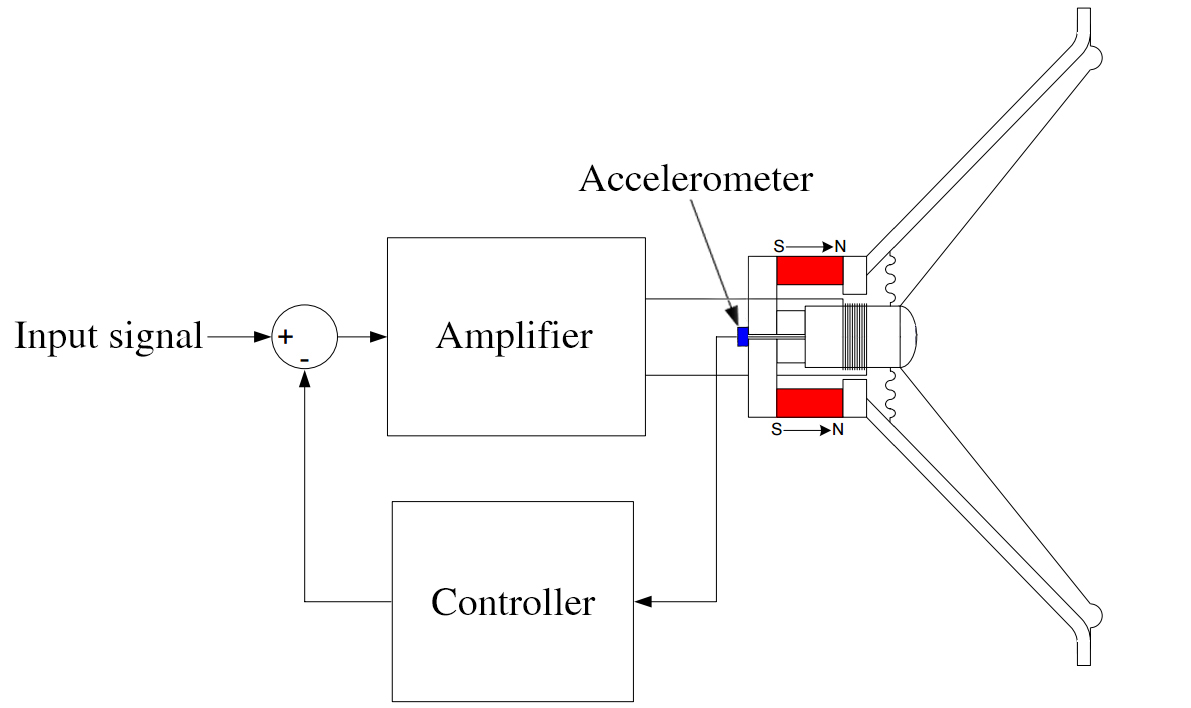
\includegraphics[width=0.75\textwidth]{Feedback_Acc2}
%\end{figure}
%\end{frame}
%
%\subsection{Analyse}
%\begin{frame}{Feedback system}{Analyse}
%Lineært sweep fra 2400 til 0 Hz
%\begin{figure}
%\centering
%\begin{subfigure}[t]{0.45\textwidth}
%\centering
%%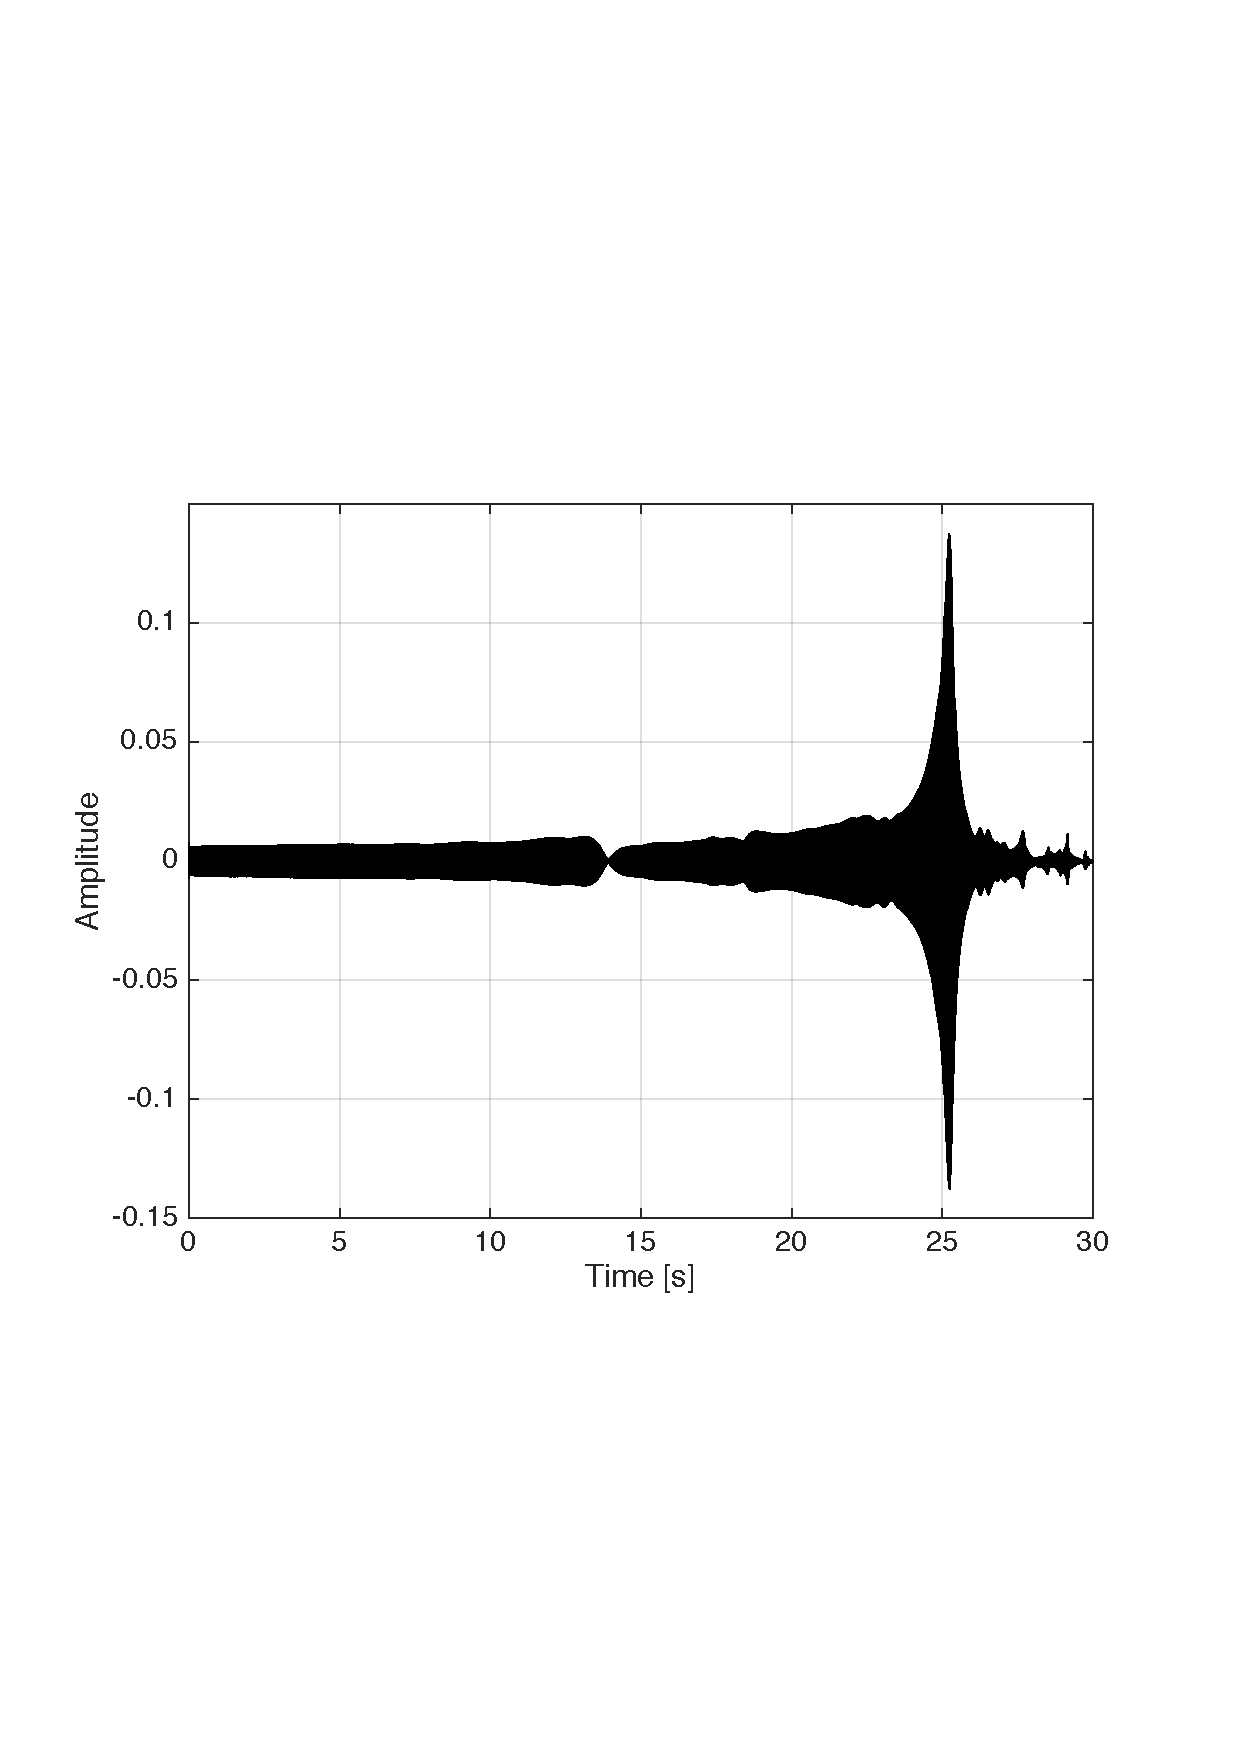
\includegraphics[width=\textwidth]{raw_driver10}
%% This file was created by matlab2tikz.
%
%The latest updates can be retrieved from
%  http://www.mathworks.com/matlabcentral/fileexchange/22022-matlab2tikz-matlab2tikz
%where you can also make suggestions and rate matlab2tikz.
%
\begin{tikzpicture}

\begin{axis}[%
width=5.521in,
height=2in,
at={(0.758in,0.481in)},
xmin=0,
xmax=30,
xmajorgrids,
ymin=-0.15,
ymax=0.15,
ymajorgrids,
axis background/.style={fill=white}
]
\addplot[fill=black,draw=black,forget plot] plot table[row sep=crcr]{%
2.08333333333333e-05	0.0119891166687012\\
0.0425739952718676	0.0120701789855957\\
0.0851271572104019	0.0120600461959839\\
0.127680319148936	0.0121411085128784\\
0.17023348108747	0.0122112035751343\\
0.212786643026005	0.0122820138931274\\
0.255339804964539	0.0123153924942017\\
0.297892966903073	0.0123672485351563\\
0.340446128841608	0.0123822689056396\\
0.382999290780142	0.0124343633651733\\
0.425552452718676	0.012420654296875\\
0.46810561465721	0.0124455690383911\\
0.510658776595745	0.0124385356903076\\
0.553211938534279	0.0124293565750122\\
0.595765100472813	0.0124131441116333\\
0.638318262411347	0.0123996734619141\\
0.680871424349882	0.0123659372329712\\
0.723424586288416	0.0123772621154785\\
0.76597774822695	0.0123530626296997\\
0.808530910165485	0.0123927593231201\\
0.851084072104019	0.0123993158340454\\
0.893637234042553	0.0123468637466431\\
0.936190395981088	0.0123317241668701\\
0.978743557919622	0.0123351812362671\\
1.02129671985816	0.0123213529586792\\
1.06384988179669	0.012315034866333\\
1.10640304373522	0.0123295783996582\\
1.14895620567376	0.0123213529586792\\
1.19150936761229	0.012312650680542\\
1.23406252955083	0.0123451948165894\\
1.27661569148936	0.0123229026794434\\
1.3191688534279	0.0123435258865356\\
1.36172201536643	0.0123484134674072\\
1.40427517730496	0.0123796463012695\\
1.4468283392435	0.0123721361160278\\
1.48938150118203	0.0123879909515381\\
1.53193466312057	0.012427806854248\\
1.5744878250591	0.0124756097793579\\
1.61704098699764	0.012513279914856\\
1.65959414893617	0.0124995708465576\\
1.7021473108747	0.0125466585159302\\
1.74470047281324	0.012596607208252\\
1.78725363475177	0.0126116275787354\\
1.82980679669031	0.0126550197601318\\
1.87235995862884	0.012694239616394\\
1.91491312056738	0.0127073526382446\\
1.95746628250591	0.0127198696136475\\
2.00001944444444	0.0127586126327515\\
2.04257260638298	0.0127676725387573\\
2.08512576832151	0.012792706489563\\
2.12767893026005	0.0128316879272461\\
2.17023209219858	0.0128744840621948\\
2.21278525413712	0.0128858089447021\\
2.25533841607565	0.0128728151321411\\
2.29789157801418	0.0128904581069946\\
2.34044473995272	0.012937068939209\\
2.38299790189125	0.0129625797271729\\
2.42555106382979	0.0129508972167969\\
2.46810422576832	0.0129650831222534\\
2.51065738770686	0.0130186080932617\\
2.55321054964539	0.0130044221878052\\
2.59576371158392	0.0130490064620972\\
2.63831687352246	0.0130782127380371\\
2.68087003546099	0.0130912065505981\\
2.72342319739953	0.0131031274795532\\
2.76597635933806	0.0131406784057617\\
2.8085295212766	0.0131857395172119\\
2.85108268321513	0.0132355690002441\\
2.89363584515366	0.0132455825805664\\
2.9361890070922	0.0132309198379517\\
2.97874216903073	0.013269305229187\\
3.02129533096927	0.0133043527603149\\
3.0638484929078	0.013329029083252\\
3.10640165484634	0.0133227109909058\\
3.14895481678487	0.0133368968963623\\
3.1915079787234	0.0133442878723145\\
3.23406114066194	0.0133599042892456\\
3.27661430260047	0.0133839845657349\\
3.31916746453901	0.0133798122406006\\
3.36172062647754	0.0133849382400513\\
3.40427378841608	0.0134093761444092\\
3.44682695035461	0.013446569442749\\
3.48938011229314	0.0134661197662354\\
3.53193327423168	0.0134836435317993\\
3.57448643617021	0.013521671295166\\
3.61703959810875	0.0135370492935181\\
3.65959276004728	0.0135470628738403\\
3.70214592198582	0.0135759115219116\\
3.74469908392435	0.0136080980300903\\
3.78725224586288	0.0136371850967407\\
3.82980540780142	0.0136731863021851\\
3.87235856973995	0.0137186050415039\\
3.91491173167849	0.0137549638748169\\
3.95746489361702	0.0137441158294678\\
4.00001805555556	0.0138174295425415\\
4.04257121749409	0.013864278793335\\
4.08512437943262	0.0139147043228149\\
4.12767754137116	0.0139368772506714\\
4.17023070330969	0.0140061378479004\\
4.21278386524823	0.0140299797058105\\
4.25533702718676	0.0140790939331055\\
4.29789018912529	0.0141112804412842\\
4.34044335106383	0.0141588449478149\\
4.38299651300236	0.0141901969909668\\
4.4255496749409	0.0142172574996948\\
4.46810283687943	0.0142718553543091\\
4.51065599881797	0.0143095254898071\\
4.5532091607565	0.0143332481384277\\
4.59576232269503	0.0143661499023438\\
4.63831548463357	0.0144078731536865\\
4.6808686465721	0.0144317150115967\\
4.72342180851064	0.014464259147644\\
4.76597497044917	0.0144739151000977\\
4.80852813238771	0.0144917964935303\\
4.85108129432624	0.0145350694656372\\
4.89363445626477	0.0145490169525146\\
4.93618761820331	0.014581561088562\\
4.97874078014184	0.0145977735519409\\
5.02129394208038	0.0146069526672363\\
5.06384710401891	0.0146232843399048\\
5.10640026595745	0.0146393775939941\\
5.14895342789598	0.0146942138671875\\
5.19150658983452	0.0146994590759277\\
5.23405975177305	0.0147175788879395\\
5.27661291371158	0.0147092342376709\\
5.31916607565012	0.0147404670715332\\
5.36171923758865	0.0147354602813721\\
5.40427239952719	0.0147433280944824\\
5.44682556146572	0.0147520303726196\\
5.48937872340426	0.0147508382797241\\
5.53193188534279	0.0147504806518555\\
5.57448504728132	0.014761209487915\\
5.61703820921986	0.0147466659545898\\
5.65959137115839	0.0147426128387451\\
5.70214453309693	0.0147403478622437\\
5.74469769503546	0.0147124528884888\\
5.787250856974	0.0147058963775635\\
5.82980401891253	0.0147024393081665\\
5.87235718085106	0.0146327018737793\\
5.9149103427896	0.0146118402481079\\
5.95746350472813	0.0145947933197021\\
6.00001666666667	0.0145722627639771\\
6.0425698286052	0.0145455598831177\\
6.08512299054374	0.0144891738891602\\
6.12767615248227	0.0144437551498413\\
6.1702293144208	0.0144070386886597\\
6.21278247635934	0.014379620552063\\
6.25533563829787	0.0143579244613647\\
6.29788880023641	0.0142805576324463\\
6.34044196217494	0.0142168998718262\\
6.38299512411347	0.014191746711731\\
6.42554828605201	0.0140836238861084\\
6.46810144799054	0.0140348672866821\\
6.51065460992908	0.0139898061752319\\
6.55320777186761	0.0139384269714355\\
6.59576093380615	0.0138537883758545\\
6.63831409574468	0.0137983560562134\\
6.68086725768321	0.0137511491775513\\
6.72342041962175	0.0137094259262085\\
6.76597358156028	0.0136710405349731\\
6.80852674349882	0.0136563777923584\\
6.85107990543735	0.0136498212814331\\
6.89363306737589	0.0136363506317139\\
6.93618622931442	0.0136944055557251\\
6.97873939125296	0.0137603282928467\\
7.02129255319149	0.0138442516326904\\
7.06384571513002	0.0139046907424927\\
7.10639887706856	0.0139477252960205\\
7.14895203900709	0.014054536819458\\
7.19150520094563	0.0141353607177734\\
7.23405836288416	0.0142430067062378\\
7.27661152482269	0.0143053531646729\\
7.31916468676123	0.014385461807251\\
7.36171784869976	0.0145281553268433\\
7.4042710106383	0.0145792961120605\\
7.44682417257683	0.0146374702453613\\
7.48937733451537	0.014722466468811\\
7.5319304964539	0.0147558450698853\\
7.57448365839243	0.0148293972015381\\
7.61703682033097	0.0148519277572632\\
7.6595899822695	0.0148772001266479\\
7.70214314420804	0.0148836374282837\\
7.74469630614657	0.0149027109146118\\
7.78724946808511	0.0148898363113403\\
7.82980263002364	0.0149227380752563\\
7.87235579196217	0.0149306058883667\\
7.91490895390071	0.0149260759353638\\
7.95746211583924	0.0149365663528442\\
8.00001527777778	0.0149394273757935\\
8.04256843971631	0.0149445533752441\\
8.08512160165485	0.0149415731430054\\
8.12767476359338	0.0149654150009155\\
8.17022792553192	0.0149649381637573\\
8.21278108747045	0.014962911605835\\
8.25533424940898	0.0149157047271729\\
8.29788741134752	0.0148886442184448\\
8.34044057328605	0.0148481130599976\\
8.38299373522459	0.0147963762283325\\
8.42554689716312	0.0147671699523926\\
8.46810005910165	0.0147316455841064\\
8.51065322104019	0.0146907567977905\\
8.55320638297872	0.0146373510360718\\
8.59575954491726	0.0146878957748413\\
8.63831270685579	0.0146653652191162\\
8.68086586879433	0.0146582126617432\\
8.72341903073286	0.0146515369415283\\
8.76597219267139	0.0146892070770264\\
8.80852535460993	0.0147384405136108\\
8.85107851654846	0.0147976875305176\\
8.893631678487	0.0148004293441772\\
8.93618484042553	0.0149153470993042\\
8.97873800236407	0.0149699449539185\\
9.0212911643026	0.0150353908538818\\
9.06384432624114	0.0150772333145142\\
9.10639748817967	0.0151313543319702\\
9.1489506501182	0.0152260065078735\\
9.19150381205674	0.0153157711029053\\
9.23405697399527	0.015323281288147\\
9.27661013593381	0.0154021978378296\\
9.31916329787234	0.0154614448547363\\
9.36171645981088	0.0155340433120728\\
9.40426962174941	0.015607476234436\\
9.44682278368794	0.015711784362793\\
9.48937594562648	0.0157406330108643\\
9.53192910756501	0.0158414840698242\\
9.57448226950355	0.0159074068069458\\
9.61703543144208	0.0159391164779663\\
9.65958859338062	0.0160180330276489\\
9.70214175531915	0.0160245895385742\\
9.74469491725768	0.0160360336303711\\
9.78724807919622	0.01607346534729\\
9.82980124113475	0.0160551071166992\\
9.87235440307329	0.0160226821899414\\
9.91490756501182	0.0159975290298462\\
9.95746072695036	0.0159332752227783\\
10.0000138888889	0.0159041881561279\\
10.0425670508274	0.0158710479736328\\
10.085120212766	0.0158164501190186\\
10.1276733747045	0.0158092975616455\\
10.170226536643	0.0157977342605591\\
10.2127796985816	0.0158299207687378\\
10.2553328605201	0.0159136056900024\\
10.2978860224586	0.0159791707992554\\
10.3404391843972	0.016069769859314\\
10.3829923463357	0.0161577463150024\\
10.4255455082742	0.0162630081176758\\
10.4680986702128	0.0163758993148804\\
10.5106518321513	0.0164648294448853\\
10.5532049940898	0.0165594816207886\\
10.5957581560284	0.0166622400283813\\
10.6383113179669	0.016768217086792\\
10.6808644799054	0.0168865919113159\\
10.723417641844	0.0169931650161743\\
10.7659708037825	0.0171152353286743\\
10.808523965721	0.0171926021575928\\
10.8510771276596	0.017282247543335\\
10.8936302895981	0.0174212455749512\\
10.9361834515366	0.0175200700759888\\
10.9787366134752	0.0176385641098022\\
11.0212897754137	0.0177961587905884\\
11.0638429373522	0.0178617238998413\\
11.1063960992908	0.0179822444915771\\
11.1489492612293	0.0180516242980957\\
11.1915024231678	0.0181763172149658\\
11.2340555851064	0.0183032751083374\\
11.2766087470449	0.0184470415115356\\
11.3191619089835	0.0185744762420654\\
11.361715070922	0.0186715126037598\\
11.4042682328605	0.0187947750091553\\
11.4468213947991	0.0189191102981567\\
11.4893745567376	0.0189660787582397\\
11.5319277186761	0.0190688371658325\\
11.5744808806147	0.019160270690918\\
11.6170340425532	0.0192372798919678\\
11.6595872044917	0.0193090438842773\\
11.7021403664303	0.019400954246521\\
11.7446935283688	0.0195177793502808\\
11.7872466903073	0.0195590257644653\\
11.8297998522459	0.0196257829666138\\
11.8723530141844	0.0197001695632935\\
11.9149061761229	0.0197663307189941\\
11.9574593380615	0.0198649168014526\\
12.0000125	0.0199562311172485\\
12.0425656619385	0.0200393199920654\\
12.0851188238771	0.0201531648635864\\
12.1276719858156	0.0202683210372925\\
12.1702251477541	0.0203834772109985\\
12.2127783096927	0.0205181837081909\\
12.2553314716312	0.0206431150436401\\
12.2978846335697	0.020803689956665\\
12.3404377955083	0.0209430456161499\\
12.3829909574468	0.0210655927658081\\
12.4255441193853	0.0211613178253174\\
12.4680972813239	0.0213009119033813\\
12.5106504432624	0.0214111804962158\\
12.5532036052009	0.0215167999267578\\
12.5957567671395	0.0215667486190796\\
12.638309929078	0.0216765403747559\\
12.6808630910165	0.0217441320419312\\
12.7234162529551	0.0217874050140381\\
12.7659694148936	0.0218304395675659\\
12.8085225768322	0.0218579769134521\\
12.8510757387707	0.0218334197998047\\
12.8936289007092	0.0218534469604492\\
12.9361820626478	0.0217874050140381\\
12.9787352245863	0.0216927528381348\\
13.0212883865248	0.021544337272644\\
13.0638415484634	0.021371603012085\\
13.1063947104019	0.0211578607559204\\
13.1489478723404	0.0209262371063232\\
13.191501034279	0.0206685066223145\\
13.2340541962175	0.0203869342803955\\
13.276607358156	0.0200080871582031\\
13.3191605200946	0.019722580909729\\
13.3617136820331	0.0194058418273926\\
13.4042668439716	0.0190954208374023\\
13.4468200059102	0.0187587738037109\\
13.4893731678487	0.0184516906738281\\
13.5319263297872	0.0181584358215332\\
13.5744794917258	0.0178221464157104\\
13.6170326536643	0.0174729824066162\\
13.6595858156028	0.0171077251434326\\
13.7021389775414	0.016639232635498\\
13.7446921394799	0.0161151885986328\\
13.7872453014184	0.0154547691345215\\
13.829798463357	0.0146360397338867\\
13.8723516252955	0.0137324333190918\\
13.914904787234	0.0126259326934814\\
13.9574579491726	0.0113997459411621\\
14.0000111111111	0.0100481510162354\\
14.0425642730496	0.00874054431915283\\
14.0851174349882	0.00763881206512451\\
14.1276705969267	0.00698995590209961\\
14.1702237588652	0.00721240043640137\\
14.2127769208038	0.0078728199005127\\
14.2553300827423	0.00864839553833008\\
14.2978832446809	0.00943124294281006\\
14.3404364066194	0.010124683380127\\
14.3829895685579	0.0107450485229492\\
14.4255427304965	0.0112762451171875\\
14.468095892435	0.0117151737213135\\
14.5106490543735	0.0120129585266113\\
14.5532022163121	0.0122971534729004\\
14.5957553782506	0.0124787092208862\\
14.6383085401891	0.0126643180847168\\
14.6808617021277	0.0127860307693481\\
14.7234148640662	0.0129104852676392\\
14.7659680260047	0.013019323348999\\
14.8085211879433	0.0130923986434937\\
14.8510743498818	0.0131598711013794\\
14.8936275118203	0.0132442712783813\\
14.9361806737589	0.0132671594619751\\
14.9787338356974	0.0133401155471802\\
15.0212869976359	0.0133960247039795\\
15.0638401595745	0.0134508609771729\\
15.106393321513	0.0134987831115723\\
15.1489464834515	0.0135847330093384\\
15.1914996453901	0.0137389898300171\\
15.2340528073286	0.0139615535736084\\
15.2766059692671	0.0141968727111816\\
15.3191591312057	0.0144667625427246\\
15.3617122931442	0.0147184133529663\\
15.4042654550827	0.0149639844894409\\
15.4468186170213	0.0151892900466919\\
15.4893717789598	0.0153195858001709\\
15.5319249408983	0.0154467821121216\\
15.5744781028369	0.0155524015426636\\
15.6170312647754	0.0156270265579224\\
15.6595844267139	0.0157109498977661\\
15.7021375886525	0.0157914161682129\\
15.744690750591	0.0158919095993042\\
15.7872439125296	0.0159846544265747\\
15.8297970744681	0.0160763263702393\\
15.8723502364066	0.0161715745925903\\
15.9149033983452	0.0162194967269897\\
15.9574565602837	0.0162959098815918\\
16.0000097222222	0.0163196325302124\\
16.0425628841608	0.0163333415985107\\
16.0851160460993	0.0164139270782471\\
16.1276692080378	0.0164852142333984\\
16.1702223699764	0.016596794128418\\
16.2127755319149	0.0167173147201538\\
16.2553286938534	0.016867995262146\\
16.297881855792	0.0169942378997803\\
16.3404350177305	0.0171358585357666\\
16.382988179669	0.017247200012207\\
16.4255413416076	0.0173672437667847\\
16.4680945035461	0.0174224376678467\\
16.5106476654846	0.0174494981765747\\
16.5532008274232	0.0174441337585449\\
16.5957539893617	0.0174261331558228\\
16.6383071513002	0.0173689126968384\\
16.6808603132388	0.017351508140564\\
16.7234134751773	0.0173255205154419\\
16.7659666371158	0.0173234939575195\\
16.8085197990544	0.0173735618591309\\
16.8510729609929	0.0174065828323364\\
16.8936261229314	0.0174649953842163\\
16.93617928487	0.017520546913147\\
16.9787324468085	0.0175772905349731\\
17.021285608747	0.017709493637085\\
17.0638387706856	0.017842173576355\\
17.1063919326241	0.0179907083511353\\
17.1489450945626	0.0182030200958252\\
17.1914982565012	0.0184568166732788\\
17.2340514184397	0.0187783241271973\\
17.2766045803783	0.0191693305969238\\
17.3191577423168	0.0196816921234131\\
17.3617109042553	0.0201215744018555\\
17.4042640661939	0.0205991268157959\\
17.4468172281324	0.0209838151931763\\
17.4893703900709	0.0212384462356567\\
17.5319235520095	0.0214720964431763\\
17.574476713948	0.0217106342315674\\
17.6170298758865	0.0218876600265503\\
17.6595830378251	0.0220842361450195\\
17.7021361997636	0.0222510099411011\\
17.7446893617021	0.0224254131317139\\
17.7872425236407	0.0225731134414673\\
17.8297956855792	0.0227036476135254\\
17.8723488475177	0.0228030681610107\\
17.9149020094563	0.0228255987167358\\
17.9574551713948	0.0227867364883423\\
18.0000083333333	0.0226969718933105\\
18.0425614952719	0.0225468873977661\\
18.0851146572104	0.022442102432251\\
18.1276678191489	0.0224337577819824\\
18.1702209810875	0.0225523710250854\\
18.212774143026	0.0226941108703613\\
18.2553273049645	0.0227112770080566\\
18.2978804669031	0.0226702690124512\\
18.3404336288416	0.0225247144699097\\
18.3829867907801	0.022191047668457\\
18.4255399527187	0.0216506719589233\\
18.4680931146572	0.0210781097412109\\
18.5106462765957	0.0205855369567871\\
18.5531994385343	0.0202169418334961\\
18.5957526004728	0.0198911428451538\\
18.6383057624113	0.0195983648300171\\
18.6808589243499	0.0192761421203613\\
18.7234120862884	0.0189481973648071\\
18.765965248227	0.0187180042266846\\
18.8085184101655	0.0185004472732544\\
18.851071572104	0.0183453559875488\\
18.8936247340426	0.0182894468307495\\
18.9361778959811	0.018202543258667\\
18.9787310579196	0.0181392431259155\\
19.0212842198582	0.018133282661438\\
19.0638373817967	0.0181257724761963\\
19.1063905437352	0.0182130336761475\\
19.1489437056738	0.0184046030044556\\
19.1914968676123	0.0186821222305298\\
19.2340500295508	0.0190776586532593\\
19.2766031914894	0.0195093154907227\\
19.3191563534279	0.0199741125106812\\
19.3617095153664	0.020482063293457\\
19.404262677305	0.0209068059921265\\
19.4468158392435	0.0214110612869263\\
19.489369001182	0.0218472480773926\\
19.5319221631206	0.0223336219787598\\
19.5744753250591	0.0227125883102417\\
19.6170284869976	0.0230491161346436\\
19.6595816489362	0.0233137607574463\\
19.7021348108747	0.0236597061157227\\
19.7446879728132	0.0238858461380005\\
19.7872411347518	0.0241514444351196\\
19.8297942966903	0.0243535041809082\\
19.8723474586288	0.0245242118835449\\
19.9149006205674	0.0246922969818115\\
19.9574537825059	0.0247610807418823\\
20.0000069444444	0.0248315334320068\\
20.042560106383	0.0248575210571289\\
20.0851132683215	0.0248454809188843\\
20.12766643026	0.0248016119003296\\
20.1702195921986	0.0247161388397217\\
20.2127727541371	0.0244866609573364\\
20.2553259160756	0.0242441892623901\\
20.2978790780142	0.0239566564559937\\
20.3404322399527	0.0237118005752563\\
20.3829854018913	0.0237652063369751\\
20.4255385638298	0.0240160226821899\\
20.4680917257683	0.0243251323699951\\
20.5106448877069	0.0246405601501465\\
20.5531980496454	0.0249805450439453\\
20.5957512115839	0.0253318548202515\\
20.6383043735225	0.025571346282959\\
20.680857535461	0.0258880853652954\\
20.7234106973995	0.0261416435241699\\
20.7659638593381	0.0264977216720581\\
20.8085170212766	0.0268567800521851\\
20.8510701832151	0.0271531343460083\\
20.8936233451537	0.0274865627288818\\
20.9361765070922	0.027751088142395\\
20.9787296690307	0.0279955863952637\\
21.0212828309693	0.0282137393951416\\
21.0638359929078	0.0284777879714966\\
21.1063891548463	0.0287666320800781\\
21.1489423167849	0.0289372205734253\\
21.1914954787234	0.0290979146957397\\
21.2340486406619	0.0291520357131958\\
21.2766018026005	0.0291374921798706\\
21.319154964539	0.0290536880493164\\
21.3617081264775	0.0289229154586792\\
21.4042612884161	0.0287134647369385\\
21.4468144503546	0.0284314155578613\\
21.4893676122931	0.0280815362930298\\
21.5319207742317	0.0277200937271118\\
21.5744739361702	0.027424693107605\\
21.6170270981087	0.0271998643875122\\
21.6595802600473	0.0271004438400269\\
21.7021334219858	0.0271096229553223\\
21.7446865839243	0.027174711227417\\
21.7872397458629	0.0272704362869263\\
21.8297929078014	0.0274029970169067\\
21.87234606974	0.0276217460632324\\
21.9148992316785	0.0278003215789795\\
21.957452393617	0.0280568599700928\\
22.0000055555556	0.028328537940979\\
22.0425587174941	0.0285825729370117\\
22.0851118794326	0.0288678407669067\\
22.1276650413712	0.0291299819946289\\
22.1702182033097	0.029487133026123\\
22.2127713652482	0.029843807220459\\
22.2553245271868	0.0302610397338867\\
22.2978776891253	0.0306540727615356\\
22.3404308510638	0.0310933589935303\\
22.3829840130024	0.0315306186676025\\
22.4255371749409	0.0319411754608154\\
22.4680903368794	0.0324456691741943\\
22.510643498818	0.0329251289367676\\
22.5531966607565	0.0331741571426392\\
22.595749822695	0.0333001613616943\\
22.6383029846336	0.0332827568054199\\
22.6808561465721	0.0331307649612427\\
22.7234093085106	0.0327298641204834\\
22.7659624704492	0.032257080078125\\
22.8085156323877	0.0318152904510498\\
22.8510687943262	0.0313825607299805\\
22.8936219562648	0.0310475826263428\\
22.9361751182033	0.0305105447769165\\
22.9787282801418	0.0299614667892456\\
23.0212814420804	0.0292130708694458\\
23.0638346040189	0.0285649299621582\\
23.1063877659574	0.0281169414520264\\
23.148940927896	0.0285003185272217\\
23.1914940898345	0.0293340682983398\\
23.234047251773	0.0306720733642578\\
23.2766004137116	0.0323584079742432\\
23.3191535756501	0.0342948436737061\\
23.3617067375887	0.0363030433654785\\
23.4042598995272	0.0377959012985229\\
23.4468130614657	0.0382936000823975\\
23.4893662234043	0.0381671190261841\\
23.5319193853428	0.0364677906036377\\
23.5744725472813	0.0325307846069336\\
23.6170257092199	0.0271339416503906\\
23.6595788711584	0.0222088098526001\\
23.7021320330969	0.0186933279037476\\
23.7446851950355	0.0165317058563232\\
23.787238356974	0.0160146951675415\\
23.8297915189125	0.0168312788009644\\
23.8723446808511	0.0176469087600708\\
23.9148978427896	0.018263578414917\\
23.9574510047281	0.018985390663147\\
24.0000041666667	0.0202053785324097\\
24.0425573286052	0.0214619636535645\\
24.0851104905437	0.022052526473999\\
24.1276636524823	0.0227371454238892\\
24.1702168144208	0.0230492353439331\\
24.2127699763593	0.0232532024383545\\
24.2553231382979	0.0234876871109009\\
24.2978763002364	0.0238732099533081\\
24.3404294621749	0.0242279767990112\\
24.3829826241135	0.0246217250823975\\
24.425535786052	0.0249172449111938\\
24.4680889479905	0.0250427722930908\\
24.5106421099291	0.0254533290863037\\
24.5531952718676	0.0256302356719971\\
24.5957484338061	0.0264087915420532\\
24.6383015957447	0.0274142026901245\\
24.6808547576832	0.028038501739502\\
24.7234079196217	0.0287498235702515\\
24.7659610815603	0.029454231262207\\
24.8085142434988	0.0302711725234985\\
24.8510674054374	0.0310555696487427\\
24.8936205673759	0.0316926240921021\\
24.9361737293144	0.0327839851379395\\
24.978726891253	0.033631443977356\\
25.0212800531915	0.0349727869033813\\
25.06383321513	0.0368019342422485\\
25.1063863770686	0.0389444828033447\\
25.1489395390071	0.041167140007019\\
25.1914927009456	0.0434926748275757\\
25.2340458628842	0.0467634201049805\\
25.2765990248227	0.0511188507080078\\
25.3191521867612	0.057016134262085\\
25.3617053486998	0.0649584531784058\\
25.4042585106383	0.0758386850357056\\
25.4468116725768	0.0889134407043457\\
25.4893648345154	0.105216860771179\\
25.5319179964539	0.116796731948853\\
25.5744711583924	0.119030594825745\\
25.617024320331	0.11763870716095\\
25.6595774822695	0.104707360267639\\
25.702130644208	0.0874937772750854\\
25.7446838061466	0.0744110345840454\\
25.7872369680851	0.06288743019104\\
25.8297901300236	0.0530766248703003\\
25.8723432919622	0.0452847480773926\\
25.9148964539007	0.0387722253799438\\
25.9574496158392	0.0343474149703979\\
26.0000027777778	0.030636191368103\\
26.0425559397163	0.0276141166687012\\
26.0851091016548	0.0244072675704956\\
26.1276622635934	0.0219786167144775\\
26.1702154255319	0.0195002555847168\\
26.2127685874705	0.017353892326355\\
26.255321749409	0.0152941942214966\\
26.2978749113475	0.0136313438415527\\
26.3404280732861	0.0135471820831299\\
26.3829812352246	0.0158743858337402\\
26.4255343971631	0.0204313993453979\\
26.4680875591017	0.0261033773422241\\
26.5106407210402	0.0301426649093628\\
26.5531938829787	0.0307470560073853\\
26.5957470449173	0.0297296047210693\\
26.6383002068558	0.0243973731994629\\
26.6808533687943	0.0204536914825439\\
26.7234065307329	0.0183995962142944\\
26.7659596926714	0.0170893669128418\\
26.8085128546099	0.0173263549804688\\
26.8510660165485	0.01812744140625\\
26.893619178487	0.0181320905685425\\
26.9361723404255	0.0170766115188599\\
26.9787255023641	0.0156316757202148\\
27.0212786643026	0.0127568244934082\\
27.0638318262411	0.0114500522613525\\
27.1063849881797	0.0104755163192749\\
27.1489381501182	0.00944781303405762\\
27.1914913120567	0.00852572917938232\\
27.2340444739953	0.00608611106872559\\
27.2765976359338	0.00501561164855957\\
27.3191507978723	0.00464582443237305\\
27.3617039598109	0.0052187442779541\\
27.4042571217494	0.00589883327484131\\
27.4468102836879	0.00653588771820068\\
27.4893634456265	0.00666952133178711\\
27.531916607565	0.00618875026702881\\
27.5744697695035	0.00481438636779785\\
27.6170229314421	0.00392997264862061\\
27.6595760933806	0.00364542007446289\\
27.7021292553192	0.00357687473297119\\
27.7446824172577	0.0039665699005127\\
27.7872355791962	0.00409770011901855\\
27.8297887411348	0.00434184074401855\\
27.8723419030733	0.00437593460083008\\
27.9148950650118	0.00416827201843262\\
27.9574482269504	0.00337409973144531\\
28.0000013888889	0.00351810455322266\\
28.0425545508274	0.00388240814208984\\
28.085107712766	0.00404250621795654\\
28.1276608747045	0.00395500659942627\\
28.170214036643	0.0031973123550415\\
28.2127671985816	0.00237417221069336\\
28.2553203605201	0.00200951099395752\\
28.2978735224586	0.00202393531799316\\
28.3404266843972	0.00191807746887207\\
28.3829798463357	0.00173366069793701\\
28.4255330082742	0.00155413150787354\\
28.4680861702128	0.00181210041046143\\
28.5106393321513	0.00211071968078613\\
28.5531924940898	0.00176608562469482\\
28.5957456560284	0.00202560424804688\\
28.6382988179669	0.00156760215759277\\
28.6808519799054	0.00219047069549561\\
28.723405141844	0.00191926956176758\\
28.7659583037825	0.00270414352416992\\
28.808511465721	0.00257468223571777\\
28.8510646276596	0.00250673294067383\\
28.8936177895981	0.00388991832733154\\
28.9361709515366	0.00561344623565674\\
28.9787241134752	0.00521004199981689\\
29.0212772754137	0.00365424156188965\\
29.0638304373522	0.0033804178237915\\
29.1063835992908	0.00262355804443359\\
29.1489367612293	0.00234818458557129\\
29.1914899231679	0.0025477409362793\\
29.2340430851064	0.00256478786468506\\
29.2765962470449	0.00208735466003418\\
29.3191494089835	0.00250005722045898\\
29.361702570922	0.00219547748565674\\
29.4042557328605	0.00211131572723389\\
29.4468088947991	0.00169658660888672\\
29.4893620567376	0.00201320648193359\\
29.5319152186761	0.00230777263641357\\
29.5744683806147	0.00270867347717285\\
29.6170215425532	0.0027766227722168\\
29.6595747044917	0.00231611728668213\\
29.7021278664303	0.00214874744415283\\
29.7446810283688	0.00160884857177734\\
29.7872341903073	0.00224554538726807\\
29.8297873522459	0.00190925598144531\\
29.8723405141844	0.00109612941741943\\
29.9148936761229	0.000704288482666016\\
29.9574468380615	0.00048518180847168\\
30	0.000414729118347168\\
}
\closedcycle;
\addplot[fill=black,draw=black,forget plot] plot table[row sep=crcr]{%
2.08333333333333e-05	-0.012113094329834\\
0.0425739952718676	-0.0121138095855713\\
0.0851271572104019	-0.0121619701385498\\
0.127680319148936	-0.0122429132461548\\
0.17023348108747	-0.0122907161712646\\
0.212786643026005	-0.0123883485794067\\
0.255339804964539	-0.0124168395996094\\
0.297892966903073	-0.0124434232711792\\
0.340446128841608	-0.01246178150177\\
0.382999290780142	-0.0125032663345337\\
0.425552452718676	-0.0125099420547485\\
0.46810561465721	-0.0125166177749634\\
0.510658776595745	-0.0125166177749634\\
0.553211938534279	-0.0125176906585693\\
0.595765100472813	-0.0125076770782471\\
0.638318262411347	-0.0125123262405396\\
0.680871424349882	-0.0124843120574951\\
0.723424586288416	-0.0124874114990234\\
0.76597774822695	-0.0124468803405762\\
0.808530910165485	-0.0124509334564209\\
0.851084072104019	-0.0124367475509644\\
0.893637234042553	-0.0124189853668213\\
0.936190395981088	-0.012392520904541\\
0.978743557919622	-0.0124033689498901\\
1.02129671985816	-0.0123730897903442\\
1.06384988179669	-0.0124198198318481\\
1.10640304373522	-0.0123876333236694\\
1.14895620567376	-0.0124117136001587\\
1.19150936761229	-0.0123980045318604\\
1.23406252955083	-0.0124258995056152\\
1.27661569148936	-0.012415885925293\\
1.3191688534279	-0.0124626159667969\\
1.36172201536643	-0.012446403503418\\
1.40427517730496	-0.0124740600585938\\
1.4468283392435	-0.0124877691268921\\
1.48938150118203	-0.0125036239624023\\
1.53193466312057	-0.0125057697296143\\
1.5744878250591	-0.0125240087509155\\
1.61704098699764	-0.0125665664672852\\
1.65959414893617	-0.012586236000061\\
1.7021473108747	-0.0126203298568726\\
1.74470047281324	-0.0126328468322754\\
1.78725363475177	-0.0126634836196899\\
1.82980679669031	-0.0127276182174683\\
1.87235995862884	-0.0127447843551636\\
1.91491312056738	-0.0127626657485962\\
1.95746628250591	-0.0127805471420288\\
2.00001944444444	-0.0128178596496582\\
2.04257260638298	-0.0128737688064575\\
2.08512576832151	-0.0128716230392456\\
2.12767893026005	-0.0129257440567017\\
2.17023209219858	-0.0129240751266479\\
2.21278525413712	-0.0129307508468628\\
2.25533841607565	-0.0129609107971191\\
2.29789157801418	-0.0129433870315552\\
2.34044473995272	-0.0129650831222534\\
2.38299790189125	-0.012988805770874\\
2.42555106382979	-0.013023853302002\\
2.46810422576832	-0.0130585432052612\\
2.51065738770686	-0.0130890607833862\\
2.55321054964539	-0.0130822658538818\\
2.59576371158392	-0.0131436586380005\\
2.63831687352246	-0.0131477117538452\\
2.68087003546099	-0.0131758451461792\\
2.72342319739953	-0.0131961107254028\\
2.76597635933806	-0.0131841897964478\\
2.8085295212766	-0.0132342576980591\\
2.85108268321513	-0.0132158994674683\\
2.89363584515366	-0.0132571458816528\\
2.9361890070922	-0.0132758617401123\\
2.97874216903073	-0.0133143663406372\\
3.02129533096927	-0.0133262872695923\\
3.0638484929078	-0.0133285522460938\\
3.10640165484634	-0.0133302211761475\\
3.14895481678487	-0.0133769512176514\\
3.1915079787234	-0.0133914947509766\\
3.23406114066194	-0.013434886932373\\
3.27661430260047	-0.0134336948394775\\
3.31916746453901	-0.0134991407394409\\
3.36172062647754	-0.0134928226470947\\
3.40427378841608	-0.0135328769683838\\
3.44682695035461	-0.0135462284088135\\
3.48938011229314	-0.0136126279830933\\
3.53193327423168	-0.0136435031890869\\
3.57448643617021	-0.0136560201644897\\
3.61703959810875	-0.0137197971343994\\
3.65959276004728	-0.0137335062026978\\
3.70214592198582	-0.0137761831283569\\
3.74469908392435	-0.013823390007019\\
3.78725224586288	-0.0138667821884155\\
3.82980540780142	-0.0138909816741943\\
3.87235856973995	-0.0139669179916382\\
3.91491173167849	-0.013978123664856\\
3.95746489361702	-0.0140331983566284\\
4.00001805555556	-0.0140602588653564\\
4.04257121749409	-0.0141162872314453\\
4.08512437943262	-0.0141328573226929\\
4.12767754137116	-0.0141587257385254\\
4.17023070330969	-0.0142300128936768\\
4.21278386524823	-0.0142171382904053\\
4.25533702718676	-0.0142806768417358\\
4.29789018912529	-0.0142964124679565\\
4.34044335106383	-0.0143094062805176\\
4.38299651300236	-0.014351487159729\\
4.4255496749409	-0.0144045352935791\\
4.46810283687943	-0.0144202709197998\\
4.51065599881797	-0.0144541263580322\\
4.5532091607565	-0.0145096778869629\\
4.59576232269503	-0.0145117044448853\\
4.63831548463357	-0.0145535469055176\\
4.6808686465721	-0.0145788192749023\\
4.72342180851064	-0.0146294832229614\\
4.76597497044917	-0.0146406888961792\\
4.80852813238771	-0.0146827697753906\\
4.85108129432624	-0.0147362947463989\\
4.89363445626477	-0.0147140026092529\\
4.93618761820331	-0.014751672744751\\
4.97874078014184	-0.0147874355316162\\
5.02129394208038	-0.0148072242736816\\
5.06384710401891	-0.0147817134857178\\
5.10640026595745	-0.0148316621780396\\
5.14895342789598	-0.0148299932479858\\
5.19150658983452	-0.0148706436157227\\
5.23405975177305	-0.0148839950561523\\
5.27661291371158	-0.0149160623550415\\
5.31916607565012	-0.0149294137954712\\
5.36171923758865	-0.0149381160736084\\
5.40427239952719	-0.0149247646331787\\
5.44682556146572	-0.0149132013320923\\
5.48937872340426	-0.0149377584457397\\
5.53193188534279	-0.014884352684021\\
5.57448504728132	-0.0148860216140747\\
5.61703820921986	-0.0148693323135376\\
5.65959137115839	-0.0148825645446777\\
5.70214453309693	-0.0148489475250244\\
5.74469769503546	-0.0148134231567383\\
5.787250856974	-0.0148054361343384\\
5.82980401891253	-0.0147805213928223\\
5.87235718085106	-0.0147774219512939\\
5.9149103427896	-0.014757513999939\\
5.95746350472813	-0.014722466468811\\
6.00001666666667	-0.0146836042404175\\
6.0425698286052	-0.0146520137786865\\
6.08512299054374	-0.0146064758300781\\
6.12767615248227	-0.0145918130874634\\
6.1702293144208	-0.0145655870437622\\
6.21278247635934	-0.0145376920700073\\
6.25533563829787	-0.0144726037979126\\
6.29788880023641	-0.0144317150115967\\
6.34044196217494	-0.0143640041351318\\
6.38299512411347	-0.0143401622772217\\
6.42554828605201	-0.0142568349838257\\
6.46810144799054	-0.0141904354095459\\
6.51065460992908	-0.014129638671875\\
6.55320777186761	-0.0140664577484131\\
6.59576093380615	-0.0139951705932617\\
6.63831409574468	-0.0139943361282349\\
6.68086725768321	-0.013921856880188\\
6.72342041962175	-0.0138674974441528\\
6.76597358156028	-0.0138700008392334\\
6.80852674349882	-0.0138266086578369\\
6.85107990543735	-0.0138033628463745\\
6.89363306737589	-0.0138267278671265\\
6.93618622931442	-0.0138603448867798\\
6.97873939125296	-0.0139093399047852\\
7.02129255319149	-0.0139569044113159\\
7.06384571513002	-0.0140078067779541\\
7.10639887706856	-0.0141046047210693\\
7.14895203900709	-0.0142216682434082\\
7.19150520094563	-0.0143018960952759\\
7.23405836288416	-0.014325737953186\\
7.27661152482269	-0.0144776105880737\\
7.31916468676123	-0.014553427696228\\
7.36171784869976	-0.0146636962890625\\
7.4042710106383	-0.0147805213928223\\
7.44682417257683	-0.0147774219512939\\
7.48937733451537	-0.0148789882659912\\
7.5319304964539	-0.014926552772522\\
7.57448365839243	-0.0149526596069336\\
7.61703682033097	-0.0149977207183838\\
7.6595899822695	-0.0150274038314819\\
7.70214314420804	-0.0150216817855835\\
7.74469630614657	-0.0150569677352905\\
7.78724946808511	-0.0150774717330933\\
7.82980263002364	-0.0150794982910156\\
7.87235579196217	-0.0150913000106812\\
7.91490895390071	-0.0150800943374634\\
7.95746211583924	-0.0151046514511108\\
8.00001527777778	-0.0151209831237793\\
8.04256843971631	-0.0151158571243286\\
8.08512160165485	-0.0151230096817017\\
8.12767476359338	-0.0151163339614868\\
8.17022792553192	-0.0151170492172241\\
8.21278108747045	-0.015113353729248\\
8.25533424940898	-0.0150854587554932\\
8.29788741134752	-0.0150784254074097\\
8.34044057328605	-0.014992356300354\\
8.38299373522459	-0.0149698257446289\\
8.42554689716312	-0.0149426460266113\\
8.46810005910165	-0.014917254447937\\
8.51065322104019	-0.0148546695709229\\
8.55320638297872	-0.014845609664917\\
8.59575954491726	-0.0148199796676636\\
8.63831270685579	-0.014836311340332\\
8.68086586879433	-0.0148338079452515\\
8.72341903073286	-0.01482093334198\\
8.76597219267139	-0.0148725509643555\\
8.80852535460993	-0.0149130821228027\\
8.85107851654846	-0.0149532556533813\\
8.893631678487	-0.0150277614593506\\
8.93618484042553	-0.0150550603866577\\
8.97873800236407	-0.0151125192642212\\
9.0212911643026	-0.0151705741882324\\
9.06384432624114	-0.0152268409729004\\
9.10639748817967	-0.0152989625930786\\
9.1489506501182	-0.0153621435165405\\
9.19150381205674	-0.0154212713241577\\
9.23405697399527	-0.0154908895492554\\
9.27661013593381	-0.0155407190322876\\
9.31916329787234	-0.0156335830688477\\
9.36171645981088	-0.0156954526901245\\
9.40426962174941	-0.0157989263534546\\
9.44682278368794	-0.0158728361129761\\
9.48937594562648	-0.0159257650375366\\
9.53192910756501	-0.0159800052642822\\
9.57448226950355	-0.0160501003265381\\
9.61703543144208	-0.0160759687423706\\
9.65958859338062	-0.0161364078521729\\
9.70214175531915	-0.0161623954772949\\
9.74469491725768	-0.0161715745925903\\
9.78724807919622	-0.0161818265914917\\
9.82980124113475	-0.0161776542663574\\
9.87235440307329	-0.0161452293395996\\
9.91490756501182	-0.0161435604095459\\
9.95746072695036	-0.0160480737686157\\
10.0000138888889	-0.0160074234008789\\
10.0425670508274	-0.0159573554992676\\
10.085120212766	-0.0158952474594116\\
10.1276733747045	-0.0158969163894653\\
10.170226536643	-0.0158489942550659\\
10.2127796985816	-0.0158857107162476\\
10.2553328605201	-0.0159428119659424\\
10.2978860224586	-0.0159850120544434\\
10.3404391843972	-0.0160963535308838\\
10.3829923463357	-0.0161405801773071\\
10.4255455082742	-0.0162266492843628\\
10.4680986702128	-0.0163537263870239\\
10.5106518321513	-0.016463041305542\\
10.5532049940898	-0.0165412425994873\\
10.5957581560284	-0.0166654586791992\\
10.6383113179669	-0.0167874097824097\\
10.6808644799054	-0.0168699026107788\\
10.723417641844	-0.0170114040374756\\
10.7659708037825	-0.0171157121658325\\
10.808523965721	-0.0172432661056519\\
10.8510771276596	-0.0173588991165161\\
10.8936302895981	-0.0174890756607056\\
10.9361834515366	-0.0176196098327637\\
10.9787366134752	-0.0177257061004639\\
11.0212897754137	-0.0178505182266235\\
11.0638429373522	-0.0179296731948853\\
11.1063960992908	-0.0180578231811523\\
11.1489492612293	-0.0181858539581299\\
11.1915024231678	-0.0183118581771851\\
11.2340555851064	-0.0184283256530762\\
11.2766087470449	-0.0185163021087646\\
11.3191619089835	-0.0186553001403809\\
11.361715070922	-0.018781304359436\\
11.4042682328605	-0.0188863277435303\\
11.4468213947991	-0.0190004110336304\\
11.4893745567376	-0.0191012620925903\\
11.5319277186761	-0.0192080736160278\\
11.5744808806147	-0.0192803144454956\\
11.6170340425532	-0.0193767547607422\\
11.6595872044917	-0.019465446472168\\
11.7021403664303	-0.0195423364639282\\
11.7446935283688	-0.0196044445037842\\
11.7872466903073	-0.0196491479873657\\
11.8297998522459	-0.0197625160217285\\
11.8723530141844	-0.019813060760498\\
11.9149061761229	-0.0199345350265503\\
11.9574593380615	-0.0199878215789795\\
12.0000125	-0.0200809240341187\\
12.0425656619385	-0.020203709602356\\
12.0851188238771	-0.0202950239181519\\
12.1276719858156	-0.0203992128372192\\
12.1702251477541	-0.0205478668212891\\
12.2127783096927	-0.0206730365753174\\
12.2553314716312	-0.0208123922348022\\
12.2978846335697	-0.0209157466888428\\
12.3404377955083	-0.0210793018341064\\
12.3829909574468	-0.0212075710296631\\
12.4255441193853	-0.0213204622268677\\
12.4680972813239	-0.0214297771453857\\
12.5106504432624	-0.0215437412261963\\
12.5532036052009	-0.0216523408889771\\
12.5957567671395	-0.0217057466506958\\
12.638309929078	-0.0217827558517456\\
12.6808630910165	-0.0218445062637329\\
12.7234162529551	-0.0219008922576904\\
12.7659694148936	-0.0219255685806274\\
12.8085225768322	-0.0219546556472778\\
12.8510757387707	-0.0219559669494629\\
12.8936289007092	-0.0219188928604126\\
12.9361820626478	-0.0218608379364014\\
12.9787352245863	-0.0217357873916626\\
13.0212883865248	-0.0215924978256226\\
13.0638415484634	-0.0214599370956421\\
13.1063947104019	-0.0211890935897827\\
13.1489478723404	-0.0209450721740723\\
13.191501034279	-0.0206962823867798\\
13.2340541962175	-0.0204030275344849\\
13.276607358156	-0.0200580358505249\\
13.3191605200946	-0.0197618007659912\\
13.3617136820331	-0.0194422006607056\\
13.4042668439716	-0.0191107988357544\\
13.4468200059102	-0.0188400745391846\\
13.4893731678487	-0.0184996128082275\\
13.5319263297872	-0.0182305574417114\\
13.5744794917258	-0.0179266929626465\\
13.6170326536643	-0.017613410949707\\
13.6595858156028	-0.0172340869903564\\
13.7021389775414	-0.0167717933654785\\
13.7446921394799	-0.0162343978881836\\
13.7872453014184	-0.0155785083770752\\
13.829798463357	-0.0147982835769653\\
13.8723516252955	-0.0138078927993774\\
13.914904787234	-0.0126904249191284\\
13.9574579491726	-0.0114437341690063\\
14.0000111111111	-0.0101087093353271\\
14.0425642730496	-0.00886237621307373\\
14.0851174349882	-0.00769996643066406\\
14.1276705969267	-0.00697076320648193\\
14.1702237588652	-0.00723934173583984\\
14.2127769208038	-0.0079423189163208\\
14.2553300827423	-0.00873672962188721\\
14.2978832446809	-0.00956249237060547\\
14.3404364066194	-0.010346531867981\\
14.3829895685579	-0.0109330415725708\\
14.4255427304965	-0.0114353895187378\\
14.468095892435	-0.0118498802185059\\
14.5106490543735	-0.0122239589691162\\
14.5532022163121	-0.0124701261520386\\
14.5957553782506	-0.0126818418502808\\
14.6383085401891	-0.0128611326217651\\
14.6808617021277	-0.0129830837249756\\
14.7234148640662	-0.013073205947876\\
14.7659680260047	-0.0131728649139404\\
14.8085211879433	-0.0132454633712769\\
14.8510743498818	-0.0133155584335327\\
14.8936275118203	-0.0134053230285645\\
14.9361806737589	-0.0134707689285278\\
14.9787338356974	-0.013554573059082\\
15.0212869976359	-0.0136101245880127\\
15.0638401595745	-0.0136501789093018\\
15.106393321513	-0.0137456655502319\\
15.1489464834515	-0.0138136148452759\\
15.1914996453901	-0.0139260292053223\\
15.2340528073286	-0.0141358375549316\\
15.2766059692671	-0.0143586397171021\\
15.3191591312057	-0.0146870613098145\\
15.3617122931442	-0.0149590969085693\\
15.4042654550827	-0.0151717662811279\\
15.4468186170213	-0.0154045820236206\\
15.4893717789598	-0.0155810117721558\\
15.5319249408983	-0.015711784362793\\
15.5744781028369	-0.0158271789550781\\
15.6170312647754	-0.0158728361129761\\
15.6595844267139	-0.0159279108047485\\
15.7021375886525	-0.016033411026001\\
15.744690750591	-0.016116738319397\\
15.7872439125296	-0.0162032842636108\\
15.8297970744681	-0.016295313835144\\
15.8723502364066	-0.0163846015930176\\
15.9149033983452	-0.0164285898208618\\
15.9574565602837	-0.016472339630127\\
16.0000097222222	-0.0165252685546875\\
16.0425628841608	-0.0165561437606812\\
16.0851160460993	-0.0166240930557251\\
16.1276692080378	-0.0167051553726196\\
16.1702223699764	-0.0168216228485107\\
16.2127755319149	-0.0169605016708374\\
16.2553286938534	-0.0171339511871338\\
16.297881855792	-0.017236590385437\\
16.3404350177305	-0.0173897743225098\\
16.382988179669	-0.0175108909606934\\
16.4255413416076	-0.0175718069076538\\
16.4680945035461	-0.0176539421081543\\
16.5106476654846	-0.0177140235900879\\
16.5532008274232	-0.0177189111709595\\
16.5957539893617	-0.0176827907562256\\
16.6383071513002	-0.0176247358322144\\
16.6808603132388	-0.0176045894622803\\
16.7234134751773	-0.0175678730010986\\
16.7659666371158	-0.0176085233688354\\
16.8085197990544	-0.0176388025283813\\
16.8510729609929	-0.0176856517791748\\
16.8936261229314	-0.0177114009857178\\
16.93617928487	-0.0177881717681885\\
16.9787324468085	-0.0179146528244019\\
17.021285608747	-0.0179815292358398\\
17.0638387706856	-0.0181503295898438\\
17.1063919326241	-0.0182839632034302\\
17.1489450945626	-0.0185275077819824\\
17.1914982565012	-0.0188034772872925\\
17.2340514184397	-0.019094705581665\\
17.2766045803783	-0.0195196866989136\\
17.3191577423168	-0.0200101137161255\\
17.3617109042553	-0.0204836130142212\\
17.4042640661939	-0.0209158658981323\\
17.4468172281324	-0.0212987661361694\\
17.4893703900709	-0.0215929746627808\\
17.5319235520095	-0.021852970123291\\
17.574476713948	-0.0220389366149902\\
17.6170298758865	-0.0222564935684204\\
17.6595830378251	-0.0223824977874756\\
17.7021361997636	-0.0225727558135986\\
17.7446893617021	-0.0228184461593628\\
17.7872425236407	-0.022945761680603\\
17.8297956855792	-0.0230010747909546\\
17.8723488475177	-0.0231268405914307\\
17.9149020094563	-0.023140549659729\\
17.9574551713948	-0.0230916738510132\\
18.0000083333333	-0.0230250358581543\\
18.0425614952719	-0.0228646993637085\\
18.0851146572104	-0.0227128267288208\\
18.1276678191489	-0.0227124691009521\\
18.1702209810875	-0.02284836769104\\
18.212774143026	-0.0229490995407104\\
18.2553273049645	-0.0229932069778442\\
18.2978804669031	-0.0229518413543701\\
18.3404336288416	-0.0227921009063721\\
18.3829867907801	-0.0224471092224121\\
18.4255399527187	-0.0218509435653687\\
18.4680931146572	-0.0213072299957275\\
18.5106462765957	-0.0208621025085449\\
18.5531994385343	-0.020465612411499\\
18.5957526004728	-0.0201561450958252\\
18.6383057624113	-0.0198447704315186\\
18.6808589243499	-0.019536018371582\\
18.7234120862884	-0.0192290544509888\\
18.765965248227	-0.019008994102478\\
18.8085184101655	-0.0188168287277222\\
18.851071572104	-0.0186343193054199\\
18.8936247340426	-0.0186009407043457\\
18.9361778959811	-0.0185483694076538\\
18.9787310579196	-0.0185364484786987\\
19.0212842198582	-0.018534779548645\\
19.0638373817967	-0.0185306072235107\\
19.1063905437352	-0.0186336040496826\\
19.1489437056738	-0.0188100337982178\\
19.1914968676123	-0.0191055536270142\\
19.2340500295508	-0.0194660425186157\\
19.2766031914894	-0.0199325084686279\\
19.3191563534279	-0.0204150676727295\\
19.3617095153664	-0.0209709405899048\\
19.404262677305	-0.0214064121246338\\
19.4468158392435	-0.0218608379364014\\
19.489369001182	-0.0222972631454468\\
19.5319221631206	-0.0227186679840088\\
19.5744753250591	-0.0231914520263672\\
19.6170284869976	-0.0235624313354492\\
19.6595816489362	-0.0238556861877441\\
19.7021348108747	-0.024156928062439\\
19.7446879728132	-0.0243837833404541\\
19.7872411347518	-0.0246430635452271\\
19.8297942966903	-0.0248475074768066\\
19.8723474586288	-0.0250301361083984\\
19.9149006205674	-0.0251462459564209\\
19.9574537825059	-0.0252714157104492\\
20.0000069444444	-0.0253260135650635\\
20.042560106383	-0.0253632068634033\\
20.0851132683215	-0.0253657102584839\\
20.12766643026	-0.0252941846847534\\
20.1702195921986	-0.0252175331115723\\
20.2127727541371	-0.0249605178833008\\
20.2553259160756	-0.0246913433074951\\
20.2978790780142	-0.0244394540786743\\
20.3404322399527	-0.0242527723312378\\
20.3829854018913	-0.0242507457733154\\
20.4255385638298	-0.0244895219802856\\
20.4680917257683	-0.024840235710144\\
20.5106448877069	-0.0251890420913696\\
20.5531980496454	-0.0255438089370728\\
20.5957512115839	-0.0258784294128418\\
20.6383043735225	-0.0261416435241699\\
20.680857535461	-0.0264842510223389\\
20.7234106973995	-0.0267868041992188\\
20.7659638593381	-0.0270984172821045\\
20.8085170212766	-0.0274379253387451\\
20.8510701832151	-0.0278090238571167\\
20.8936233451537	-0.0281018018722534\\
20.9361765070922	-0.0284202098846436\\
20.9787296690307	-0.0285882949829102\\
21.0212828309693	-0.0288512706756592\\
21.0638359929078	-0.0291566848754883\\
21.1063891548463	-0.0294057130813599\\
21.1489423167849	-0.029560923576355\\
21.1914954787234	-0.0297291278839111\\
21.2340486406619	-0.0298041105270386\\
21.2766018026005	-0.0297858715057373\\
21.319154964539	-0.0297127962112427\\
21.3617081264775	-0.0295771360397339\\
21.4042612884161	-0.0293952226638794\\
21.4468144503546	-0.0290640592575073\\
21.4893676122931	-0.0287580490112305\\
21.5319207742317	-0.028398871421814\\
21.5744739361702	-0.0281530618667603\\
21.6170270981087	-0.0279345512390137\\
21.6595802600473	-0.0278499126434326\\
21.7021334219858	-0.0278586149215698\\
21.7446865839243	-0.0279266834259033\\
21.7872397458629	-0.028020977973938\\
21.8297929078014	-0.0281990766525269\\
21.87234606974	-0.0283629894256592\\
21.9148992316785	-0.0285482406616211\\
21.957452393617	-0.0287092924118042\\
22.0000055555556	-0.0289257764816284\\
22.0425587174941	-0.0292145013809204\\
22.0851118794326	-0.0294464826583862\\
22.1276650413712	-0.0297435522079468\\
22.1702182033097	-0.0299822092056274\\
22.2127713652482	-0.0302914381027222\\
22.2553245271868	-0.0306106805801392\\
22.2978776891253	-0.0309257507324219\\
22.3404308510638	-0.0312914848327637\\
22.3829840130024	-0.0317167043685913\\
22.4255371749409	-0.0321499109268188\\
22.4680903368794	-0.0325453281402588\\
22.510643498818	-0.0331461429595947\\
22.5531966607565	-0.0333998203277588\\
22.595749822695	-0.0335463285446167\\
22.6383029846336	-0.0334912538528442\\
22.6808561465721	-0.033268928527832\\
22.7234093085106	-0.0329042673110962\\
22.7659624704492	-0.0324686765670776\\
22.8085156323877	-0.0319713354110718\\
22.8510687943262	-0.0315302610397339\\
22.8936219562648	-0.0311537981033325\\
22.9361751182033	-0.03062903881073\\
22.9787282801418	-0.0301278829574585\\
23.0212814420804	-0.0293489694595337\\
23.0638346040189	-0.0287497043609619\\
23.1063877659574	-0.0283768177032471\\
23.148940927896	-0.0287985801696777\\
23.1914940898345	-0.0296826362609863\\
23.234047251773	-0.0311105251312256\\
23.2766004137116	-0.0328836441040039\\
23.3191535756501	-0.0349277257919312\\
23.3617067375887	-0.0369383096694946\\
23.4042598995272	-0.0384221076965332\\
23.4468130614657	-0.0387804508209229\\
23.4893662234043	-0.0386364459991455\\
23.5319193853428	-0.0366133451461792\\
23.5744725472813	-0.0324814319610596\\
23.6170257092199	-0.0272306203842163\\
23.6595788711584	-0.0230542421340942\\
23.7021320330969	-0.0204013586044312\\
23.7446851950355	-0.0188719034194946\\
23.787238356974	-0.0178704261779785\\
23.8297915189125	-0.0171127319335938\\
23.8723446808511	-0.0162925720214844\\
23.9148978427896	-0.0170848369598389\\
23.9574510047281	-0.0185630321502686\\
24.0000041666667	-0.0200643539428711\\
24.0425573286052	-0.0211703777313232\\
24.0851104905437	-0.0217549800872803\\
24.1276636524823	-0.0224350690841675\\
24.1702168144208	-0.0227675437927246\\
24.2127699763593	-0.022969126701355\\
24.2553231382979	-0.0233221054077148\\
24.2978763002364	-0.023668646812439\\
24.3404294621749	-0.0239932537078857\\
24.3829826241135	-0.0243989229202271\\
24.425535786052	-0.0247251987457275\\
24.4680889479905	-0.0250644683837891\\
24.5106421099291	-0.0254218578338623\\
24.5531952718676	-0.025898814201355\\
24.5957484338061	-0.0265917778015137\\
24.6383015957447	-0.0276730060577393\\
24.6808547576832	-0.0282825231552124\\
24.7234079196217	-0.0289866924285889\\
24.7659610815603	-0.0297031402587891\\
24.8085142434988	-0.030548095703125\\
24.8510674054374	-0.0312055349349976\\
24.8936205673759	-0.031841516494751\\
24.9361737293144	-0.0328391790390015\\
24.978726891253	-0.0339288711547852\\
25.0212800531915	-0.035198450088501\\
25.06383321513	-0.0368474721908569\\
25.1063863770686	-0.0390475988388062\\
25.1489395390071	-0.0414108037948608\\
25.1914927009456	-0.0437030792236328\\
25.2340458628842	-0.0467233657836914\\
25.2765990248227	-0.0511288642883301\\
25.3191521867612	-0.0571962594985962\\
25.3617053486998	-0.0646259784698486\\
25.4042585106383	-0.0756731033325195\\
25.4468116725768	-0.0900107622146606\\
25.4893648345154	-0.106517434120178\\
25.5319179964539	-0.117760181427002\\
25.5744711583924	-0.120304703712463\\
25.617024320331	-0.118663787841797\\
25.6595774822695	-0.105951189994812\\
25.702130644208	-0.0878504514694214\\
25.7446838061466	-0.0743048191070557\\
25.7872369680851	-0.062743067741394\\
25.8297901300236	-0.0531266927719116\\
25.8723432919622	-0.0451687574386597\\
25.9148964539007	-0.0392382144927979\\
25.9574496158392	-0.0346691608428955\\
26.0000027777778	-0.0308834314346313\\
26.0425559397163	-0.0280163288116455\\
26.0851091016548	-0.0246533155441284\\
26.1276622635934	-0.022192120552063\\
26.1702154255319	-0.0199754238128662\\
26.2127685874705	-0.0176162719726563\\
26.255321749409	-0.0156316757202148\\
26.2978749113475	-0.0139467716217041\\
26.3404280732861	-0.0132524967193604\\
26.3829812352246	-0.0155760049819946\\
26.4255343971631	-0.0200768709182739\\
26.4680875591017	-0.0254929065704346\\
26.5106407210402	-0.0302547216415405\\
26.5531938829787	-0.0309668779373169\\
26.5957470449173	-0.0300536155700684\\
26.6383002068558	-0.025094747543335\\
26.6808533687943	-0.0210789442062378\\
26.7234065307329	-0.0190765857696533\\
26.7659596926714	-0.0178474187850952\\
26.8085128546099	-0.0181995630264282\\
26.8510660165485	-0.0192974805831909\\
26.893619178487	-0.0189977884292603\\
26.9361723404255	-0.0184450149536133\\
26.9787255023641	-0.0172257423400879\\
27.0212786643026	-0.0149557590484619\\
27.0638318262411	-0.0135083198547363\\
27.1063849881797	-0.0118732452392578\\
27.1489381501182	-0.00967049598693848\\
27.1914913120567	-0.00833010673522949\\
27.2340444739953	-0.00634682178497314\\
27.2765976359338	-0.00536131858825684\\
27.3191507978723	-0.00499844551086426\\
27.3617039598109	-0.00536561012268066\\
27.4042571217494	-0.00578534603118896\\
27.4468102836879	-0.00641584396362305\\
27.4893634456265	-0.00667703151702881\\
27.531916607565	-0.00637650489807129\\
27.5744697695035	-0.00545620918273926\\
27.6170229314421	-0.00457918643951416\\
27.6595760933806	-0.00394737720489502\\
27.7021292553192	-0.00365829467773438\\
27.7446824172577	-0.00367164611816406\\
27.7872355791962	-0.00402450561523438\\
27.8297887411348	-0.00435495376586914\\
27.8723419030733	-0.00426328182220459\\
27.9148950650118	-0.00445151329040527\\
27.9574482269504	-0.00378835201263428\\
28.0000013888889	-0.00349342823028564\\
28.0425545508274	-0.00329399108886719\\
28.085107712766	-0.00302791595458984\\
28.1276608747045	-0.00267183780670166\\
28.170214036643	-0.00196731090545654\\
28.2127671985816	-0.00182199478149414\\
28.2553203605201	-0.00181460380554199\\
28.2978735224586	-0.00157332420349121\\
28.3404266843972	-0.0014960765838623\\
28.3829798463357	-0.00144994258880615\\
28.4255330082742	-0.00126886367797852\\
28.4680861702128	-0.00168478488922119\\
28.5106393321513	-0.00208854675292969\\
28.5531924940898	-0.00218296051025391\\
28.5957456560284	-0.00152206420898438\\
28.6382988179669	-0.000938773155212402\\
28.6808519799054	-0.00146579742431641\\
28.723405141844	-0.000936627388000488\\
28.7659583037825	-0.00134682655334473\\
28.808511465721	-0.0016472339630127\\
28.8510646276596	-0.00189638137817383\\
28.8936177895981	-0.00312912464141846\\
28.9361709515366	-0.00524461269378662\\
28.9787241134752	-0.0041731595993042\\
29.0212772754137	-0.00321519374847412\\
29.0638304373522	-0.00288259983062744\\
29.1063835992908	-0.00251543521881104\\
29.1489367612293	-0.00225639343261719\\
29.1914899231679	-0.0026085376739502\\
29.2340430851064	-0.00243449211120605\\
29.2765962470449	-0.00240147113800049\\
29.3191494089835	-0.00282597541809082\\
29.361702570922	-0.00239741802215576\\
29.4042557328605	-0.00224804878234863\\
29.4468088947991	-0.00176239013671875\\
29.4893620567376	-0.0020139217376709\\
29.5319152186761	-0.00291180610656738\\
29.5744683806147	-0.00376307964324951\\
29.6170215425532	-0.0036391019821167\\
29.6595747044917	-0.00233137607574463\\
29.7021278664303	-0.00203859806060791\\
29.7446810283688	-0.00157201290130615\\
29.7872341903073	-0.00160586833953857\\
29.8297873522459	-0.0014573335647583\\
29.8723405141844	-0.000866174697875977\\
29.9148936761229	-0.000551462173461914\\
29.9574468380615	-0.000326752662658691\\
30	-0.000211477279663086\\
}
\closedcycle;
\end{axis}
\end{tikzpicture}%
%\caption{Accelerometer på driver - Måling 10}
%\end{subfigure}
%\begin{subfigure}[t]{0.45\textwidth}
%\centering
%%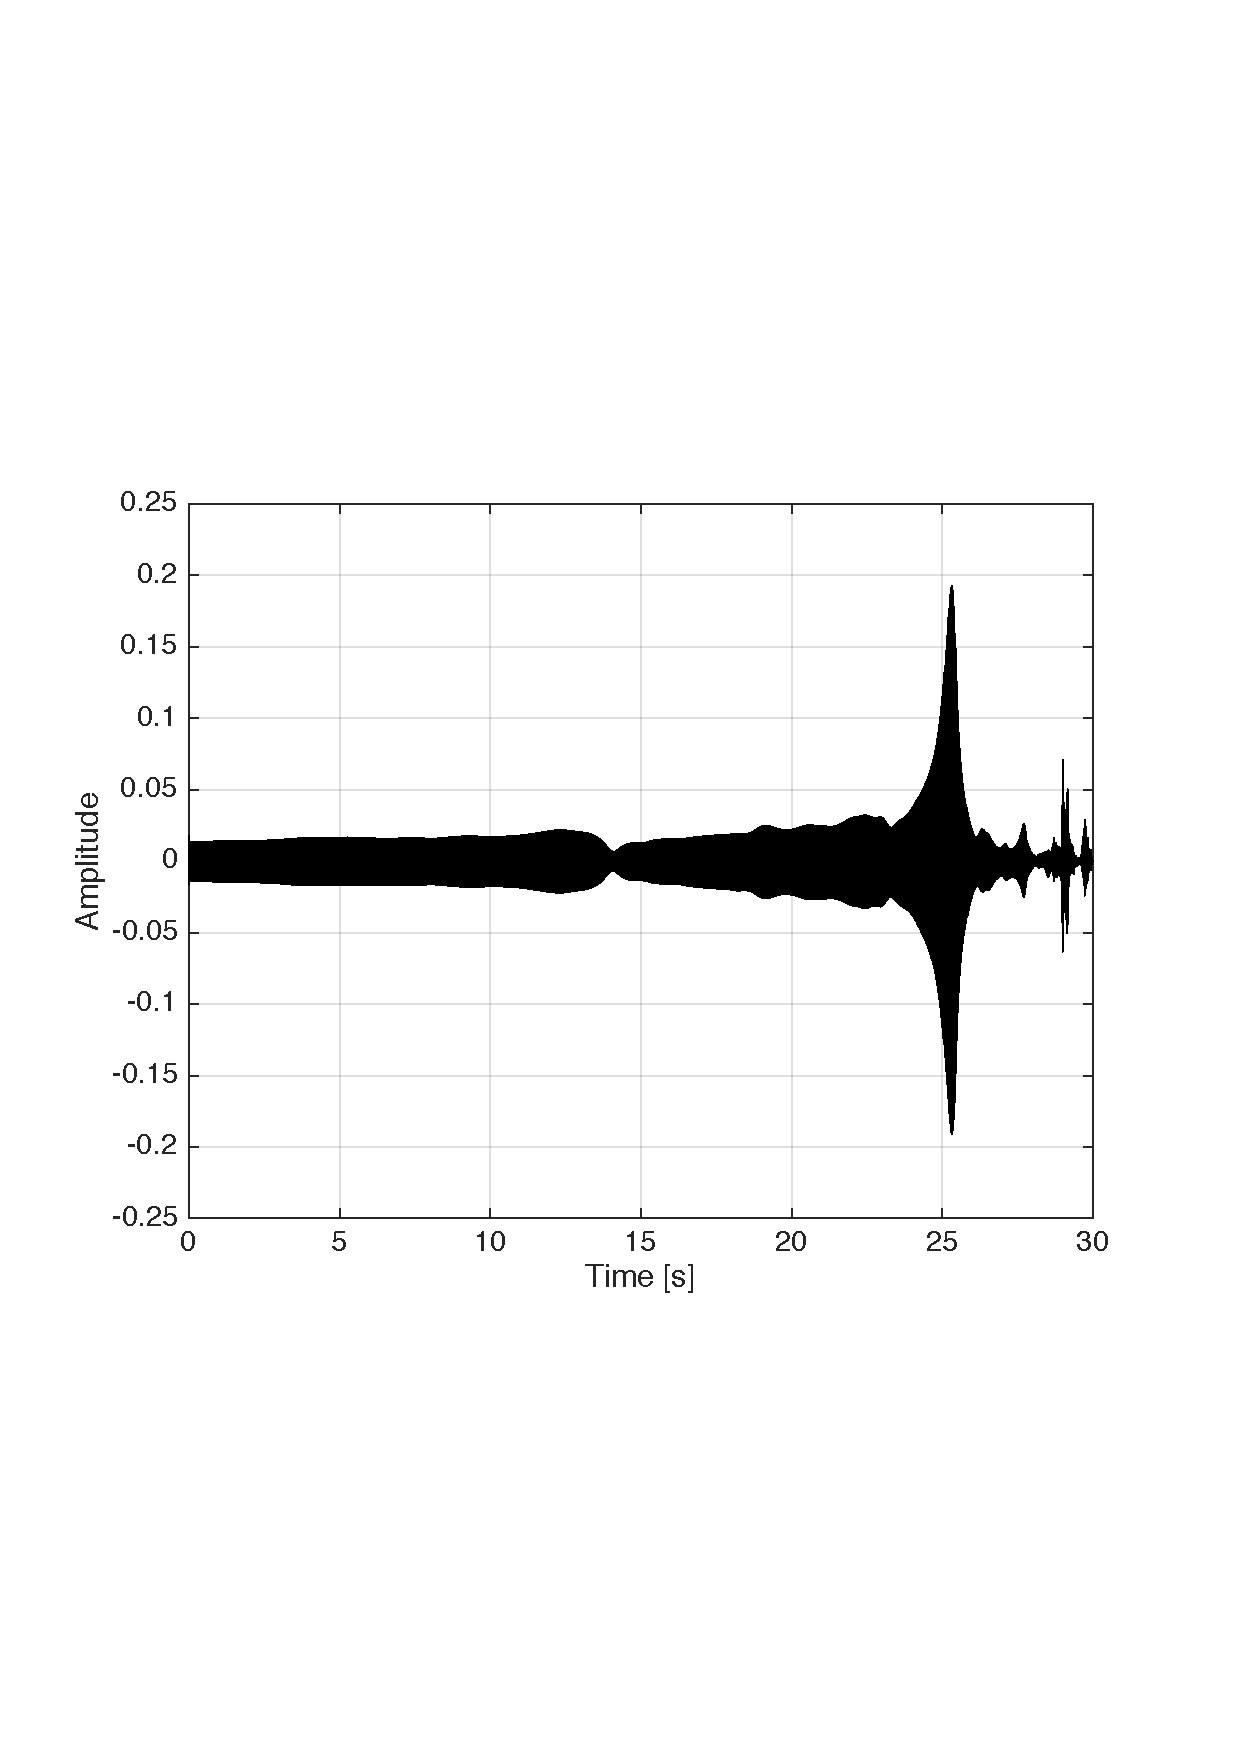
\includegraphics[width=\textwidth]{raw_driver19}
%% This file was created by matlab2tikz.
%
%The latest updates can be retrieved from
%  http://www.mathworks.com/matlabcentral/fileexchange/22022-matlab2tikz-matlab2tikz
%where you can also make suggestions and rate matlab2tikz.
%
\begin{tikzpicture}

\begin{axis}[%
width=1.6in,
height=1.2in,
at={(0.758in,0.481in)},
scale only axis,
xmin=0,
xmax=30,
xmajorgrids,
ymin=-0.2,
ymax=0.2,
ymajorgrids,
xlabel={Time [s]},
ylabel={Amplitude [V]},
axis background/.style={fill=white}
]
\addplot[fill=black,draw=black,forget plot] plot table[row sep=crcr]{%
2.08333333333333e-05	0.0174441337585449\\
0.0417454218822439	0.0131838321685791\\
0.0834700104311544	0.0131036043167114\\
0.125194598980065	0.0131006240844727\\
0.166919187528975	0.0131523609161377\\
0.208643776077886	0.0131937265396118\\
0.250368364626797	0.013242244720459\\
0.292092953175707	0.0132843255996704\\
0.333817541724618	0.0133000612258911\\
0.375542130273528	0.0133227109909058\\
0.417266718822439	0.0133814811706543\\
0.458991307371349	0.0134208202362061\\
0.50071589592026	0.0134570598602295\\
0.54244048446917	0.0134916305541992\\
0.584165073018081	0.0135313272476196\\
0.625889661566991	0.0135787725448608\\
0.667614250115902	0.0136535167694092\\
0.709338838664812	0.0136919021606445\\
0.751063427213723	0.0137407779693604\\
0.792788015762633	0.01378333568573\\
0.834512604311544	0.0138405561447144\\
0.876237192860454	0.0138554573059082\\
0.917961781409365	0.0138992071151733\\
0.959686369958275	0.0139317512512207\\
1.00141095850719	0.0139665603637695\\
1.0431355470561	0.0140010118484497\\
1.08486013560501	0.0140565633773804\\
1.12658472415392	0.0140770673751831\\
1.16830931270283	0.0141662359237671\\
1.21003390125174	0.0141417980194092\\
1.25175848980065	0.014143705368042\\
1.29348307834956	0.0142022371292114\\
1.33520766689847	0.014235258102417\\
1.37693225544738	0.0142310857772827\\
1.41865684399629	0.0142514705657959\\
1.4603814325452	0.0142501592636108\\
1.50210602109411	0.0142426490783691\\
1.54383060964302	0.0142196416854858\\
1.58555519819193	0.0141897201538086\\
1.62727978674084	0.0141717195510864\\
1.66900437528975	0.0141562223434448\\
1.71072896383866	0.0141338109970093\\
1.75245355238758	0.0141158103942871\\
1.79417814093649	0.0141069889068604\\
1.8359027294854	0.014079213142395\\
1.87762731803431	0.0140920877456665\\
1.91935190658322	0.0140824317932129\\
1.96107649513213	0.014080286026001\\
2.00280108368104	0.0140819549560547\\
2.04452567222995	0.0140804052352905\\
2.08625026077886	0.0140907764434814\\
2.12797484932777	0.0141453742980957\\
2.16969943787668	0.0141212940216064\\
2.21142402642559	0.014117956161499\\
2.2531486149745	0.0141592025756836\\
2.29487320352341	0.0141942501068115\\
2.33659779207232	0.0142147541046143\\
2.37832238062123	0.014255166053772\\
2.42004696917014	0.0142718553543091\\
2.46177155771905	0.0143097639083862\\
2.50349614626796	0.0143415927886963\\
2.54522073481687	0.0143803358078003\\
2.58694532336579	0.0144282579421997\\
2.6286699119147	0.014466404914856\\
2.67039450046361	0.0145164728164673\\
2.71211908901252	0.0145268440246582\\
2.75384367756143	0.0145998001098633\\
2.79556826611034	0.014657735824585\\
2.83729285465925	0.0147078037261963\\
2.87901744320816	0.014757513999939\\
2.92074203175707	0.0148080587387085\\
2.96246662030598	0.0148706436157227\\
3.00419120885489	0.0149272680282593\\
3.0459157974038	0.0149846076965332\\
3.08764038595271	0.0150657892227173\\
3.12936497450162	0.0151398181915283\\
3.17108956305053	0.0152368545532227\\
3.21281415159944	0.0153077840805054\\
3.25453874014835	0.0153566598892212\\
3.29626332869726	0.0154335498809814\\
3.33798791724618	0.0155411958694458\\
3.37971250579509	0.0155764818191528\\
3.421437094344	0.0156253576278687\\
3.46316168289291	0.0156955718994141\\
3.50488627144182	0.015771746635437\\
3.54661085999073	0.0158456563949585\\
3.58833544853964	0.0159142017364502\\
3.63006003708855	0.0159842967987061\\
3.67178462563746	0.0160502195358276\\
3.71350921418637	0.0160926580429077\\
3.75523380273528	0.0161477327346802\\
3.79695839128419	0.01618492603302\\
3.8386829798331	0.0162196159362793\\
3.88040756838201	0.0162382125854492\\
3.92213215693092	0.0162550210952759\\
3.96385674547983	0.0162825584411621\\
4.00558133402874	0.0162662267684937\\
4.04730592257765	0.0162646770477295\\
4.08903051112656	0.0162562131881714\\
4.13075509967547	0.0162286758422852\\
4.17247968822439	0.0162371397018433\\
4.2142042767733	0.0162320137023926\\
4.25592886532221	0.0162011384963989\\
4.29765345387112	0.0161941051483154\\
4.33937804242003	0.0161887407302856\\
4.38110263096894	0.0161789655685425\\
4.42282721951785	0.0162254571914673\\
4.46455180806676	0.0162070989608765\\
4.50627639661567	0.0162445306777954\\
4.54800098516458	0.0162758827209473\\
4.58972557371349	0.0163146257400513\\
4.6314501622624	0.0163501501083374\\
4.67317475081131	0.0163940191268921\\
4.71489933936022	0.0164343118667603\\
4.75662392790913	0.0164703130722046\\
4.79834851645804	0.0165045261383057\\
4.84007310500695	0.0165075063705444\\
4.88179769355586	0.0165128707885742\\
4.92352228210478	0.0165145397186279\\
4.96524687065368	0.0165392160415649\\
5.0069714592026	0.0165344476699829\\
5.04869604775151	0.0165383815765381\\
5.09042063630042	0.0165327787399292\\
5.13214522484933	0.0165436267852783\\
5.17386981339824	0.0165482759475708\\
5.21559440194715	0.0165524482727051\\
5.25731899049606	0.0165770053863525\\
5.29904357904497	0.0165486335754395\\
5.34076816759388	0.016539454460144\\
5.38249275614279	0.0165292024612427\\
5.4242173446917	0.0165091753005981\\
5.46594193324061	0.01650071144104\\
5.50766652178952	0.0164941549301147\\
5.54939111033843	0.0164557695388794\\
5.59111569888734	0.0164422988891602\\
5.63284028743625	0.0164107084274292\\
5.67456487598516	0.0163847208023071\\
5.71628946453407	0.0163488388061523\\
5.75801405308299	0.0162984132766724\\
5.7997386416319	0.016254186630249\\
5.84146323018081	0.0161999464035034\\
5.88318781872972	0.0161627531051636\\
5.92491240727863	0.016115665435791\\
5.96663699582754	0.0160861015319824\\
6.00836158437645	0.0160255432128906\\
6.05008617292536	0.0159963369369507\\
6.09181076147427	0.0159608125686646\\
6.13353535002318	0.015892505645752\\
6.17525993857209	0.0158644914627075\\
6.216984527121	0.0158439874649048\\
6.25870911566991	0.0158376693725586\\
6.30043370421882	0.015795111656189\\
6.34215829276773	0.0157642364501953\\
6.38388288131664	0.0157539844512939\\
6.42560746986555	0.0157680511474609\\
6.46733205841446	0.0157626867294312\\
6.50905664696338	0.0157822370529175\\
6.55078123551229	0.0157889127731323\\
6.5925058240612	0.01578688621521\\
6.63423041261011	0.015788197517395\\
6.67595500115902	0.0158027410507202\\
6.71767958970793	0.0158090591430664\\
6.75940417825684	0.0158181190490723\\
6.80112876680575	0.0158118009567261\\
6.84285335535466	0.0158218145370483\\
6.88457794390357	0.0158369541168213\\
6.92630253245248	0.0158761739730835\\
6.96802712100139	0.0158882141113281\\
7.0097517095503	0.0159152746200562\\
7.05147629809921	0.015964150428772\\
7.09320088664812	0.0159767866134644\\
7.13492547519703	0.0160250663757324\\
7.17665006374594	0.0161073207855225\\
7.21837465229485	0.0161528587341309\\
7.26009924084376	0.0162261724472046\\
7.30182382939268	0.0163071155548096\\
7.34354841794159	0.0163383483886719\\
7.3852730064905	0.016379714012146\\
7.42699759503941	0.0164109468460083\\
7.46872218358832	0.0164202451705933\\
7.51044677213723	0.01641845703125\\
7.55217136068614	0.0163893699645996\\
7.59389594923505	0.0163551568984985\\
7.63562053778396	0.016291618347168\\
7.67734512633287	0.0162198543548584\\
7.71906971488178	0.0161285400390625\\
7.76079430343069	0.016048789024353\\
7.8025188919796	0.0159471035003662\\
7.84424348052851	0.0158181190490723\\
7.88596806907742	0.0157514810562134\\
7.92769265762633	0.0156846046447754\\
7.96941724617524	0.0156430006027222\\
8.01114183472416	0.0156441926956177\\
8.05286642327307	0.015630841255188\\
8.09459101182198	0.0156680345535278\\
8.13631560037089	0.015711784362793\\
8.1780401889198	0.0157798528671265\\
8.21976477746871	0.0158299207687378\\
8.26148936601762	0.0159074068069458\\
8.30321395456653	0.0159891843795776\\
8.34493854311544	0.01605224609375\\
8.38666313166435	0.0161564350128174\\
8.42838772021326	0.0162137746810913\\
8.47011230876217	0.0163058042526245\\
8.51183689731108	0.0163658857345581\\
8.55356148585999	0.0164523124694824\\
8.5952860744089	0.0164806842803955\\
8.63701066295781	0.0166155099868774\\
8.67873525150672	0.0166575908660889\\
8.72045984005563	0.0167548656463623\\
8.76218442860454	0.016825795173645\\
8.80390901715345	0.0169020891189575\\
8.84563360570237	0.0169821977615356\\
8.88735819425128	0.0170701742172241\\
8.92908278280018	0.0171375274658203\\
8.9708073713491	0.0171587467193604\\
9.01253195989801	0.017237663269043\\
9.05425654844692	0.0172935724258423\\
9.09598113699583	0.0173218250274658\\
9.13770572554474	0.0173497200012207\\
9.17943031409365	0.0173822641372681\\
9.22115490264256	0.0174020528793335\\
9.26287949119147	0.0174028873443604\\
9.30460407974038	0.0174020528793335\\
9.34632866828929	0.017397403717041\\
9.3880532568382	0.017382025718689\\
9.42977784538711	0.0173323154449463\\
9.47150243393602	0.0173298120498657\\
9.51322702248493	0.0173071622848511\\
9.55495161103384	0.0172981023788452\\
9.59667619958275	0.0172533988952637\\
9.63840078813166	0.0172268152236938\\
9.68012537668058	0.0172126293182373\\
9.72184996522949	0.0172011852264404\\
9.7635745537784	0.0171804428100586\\
9.80529914232731	0.0171520709991455\\
9.84702373087622	0.0171386003494263\\
9.88874831942513	0.0171166658401489\\
9.93047290797404	0.0170993804931641\\
9.97219749652295	0.0170501470565796\\
10.0139220850719	0.0170356035232544\\
10.0556466736208	0.0170102119445801\\
10.0973712621697	0.0169705152511597\\
10.1390958507186	0.0169491767883301\\
10.1808204392675	0.0169264078140259\\
10.2225450278164	0.0169349908828735\\
10.2642696163653	0.016948938369751\\
10.3059942049142	0.0169826745986938\\
10.3477187934631	0.0170327425003052\\
10.3894433820121	0.0170915126800537\\
10.431167970561	0.0171574354171753\\
10.4728925591099	0.0172317028045654\\
10.5146171476588	0.0172722339630127\\
10.5563417362077	0.0173627138137817\\
10.5980663247566	0.0174278020858765\\
10.6397909133055	0.0175130367279053\\
10.6815155018544	0.0175483226776123\\
10.7232400904033	0.0176342725753784\\
10.7649646789523	0.0176903009414673\\
10.8066892675012	0.0177403688430786\\
10.8484138560501	0.0177834033966064\\
10.890138444599	0.0178585052490234\\
10.9318630331479	0.0179126262664795\\
10.9735876216968	0.0179930925369263\\
11.0153122102457	0.0180377960205078\\
11.0570367987946	0.0181233882904053\\
11.0987613873435	0.0181983709335327\\
11.1404859758924	0.0183128118515015\\
11.1822105644414	0.0184154510498047\\
11.2239351529903	0.0185511112213135\\
11.2656597415392	0.0186648368835449\\
11.3073843300881	0.0188018083572388\\
11.349108918637	0.0189625024795532\\
11.3908335071859	0.0190943479537964\\
11.4325580957348	0.0192328691482544\\
11.4742826842837	0.0194246768951416\\
11.5160072728326	0.0195508003234863\\
11.5577318613816	0.019692063331604\\
11.5994564499305	0.0198198556900024\\
11.6411810384794	0.0199755430221558\\
11.6829056270283	0.0201060771942139\\
11.7246302155772	0.0202442407608032\\
11.7663548041261	0.0203926563262939\\
11.808079392675	0.0205307006835938\\
11.8498039812239	0.0206559896469116\\
11.8915285697728	0.0208258628845215\\
11.9332531583217	0.0209463834762573\\
11.9749777468707	0.0210902690887451\\
12.0167023354196	0.0212063789367676\\
12.0584269239685	0.0213172435760498\\
12.1001515125174	0.0214052200317383\\
12.1418761010663	0.0215300321578979\\
12.1836006896152	0.0216346979141235\\
12.2253252781641	0.0217214822769165\\
12.267049866713	0.0217512845993042\\
12.3087744552619	0.0217386484146118\\
12.3504990438108	0.0217629671096802\\
12.3922236323598	0.0217190980911255\\
12.4339482209087	0.0217164754867554\\
12.4756728094576	0.0216211080551147\\
12.5173973980065	0.0215216875076294\\
12.5591219865554	0.0214111804962158\\
12.6008465751043	0.0212830305099487\\
12.6425711636532	0.0211762189865112\\
12.6842957522021	0.0210355520248413\\
12.726020340751	0.0209170579910278\\
12.7677449293	0.0208185911178589\\
12.8094695178489	0.0207177400588989\\
12.8511941063978	0.0206308364868164\\
12.8929186949467	0.0205261707305908\\
12.9346432834956	0.0204188823699951\\
12.9763678720445	0.0203160047531128\\
13.0180924605934	0.0202019214630127\\
13.0598170491423	0.020089864730835\\
13.1015416376912	0.0199722051620483\\
13.1432662262401	0.0198445320129395\\
13.1849908147891	0.0197038650512695\\
13.226715403338	0.0195189714431763\\
13.2684399918869	0.0193073749542236\\
13.3101645804358	0.0190596580505371\\
13.3518891689847	0.0188181400299072\\
13.3936137575336	0.0185122489929199\\
13.4353383460825	0.0181918144226074\\
13.4770629346314	0.0177853107452393\\
13.5187875231803	0.0173110961914063\\
13.5605121117293	0.0167787075042725\\
13.6022367002782	0.0161740779876709\\
13.6439612888271	0.0155293941497803\\
13.685685877376	0.0147796869277954\\
13.7274104659249	0.0139639377593994\\
13.7691350544738	0.0130655765533447\\
13.8108596430227	0.0121190547943115\\
13.8525842315716	0.011111855506897\\
13.8943088201205	0.0100915431976318\\
13.9360334086694	0.00906765460968018\\
13.9777579972184	0.0081101655960083\\
14.0194825857673	0.00735759735107422\\
14.0612071743162	0.00674760341644287\\
14.1029317628651	0.00652647018432617\\
14.144656351414	0.00688815116882324\\
14.1863809399629	0.00745463371276855\\
14.2281055285118	0.00815272331237793\\
14.2698301170607	0.00885546207427979\\
14.3115547056096	0.00954830646514893\\
14.3532792941586	0.0101321935653687\\
14.3950038827075	0.0106920003890991\\
14.4367284712564	0.0111517906188965\\
14.4784530598053	0.0115351676940918\\
14.5201776483542	0.0118722915649414\\
14.5619022369031	0.0121043920516968\\
14.603626825452	0.0123043060302734\\
14.6453514140009	0.0124328136444092\\
14.6870760025498	0.0125536918640137\\
14.7288005910988	0.0126279592514038\\
14.7705251796477	0.0126522779464722\\
14.8122497681966	0.0126771926879883\\
14.8539743567455	0.0126643180847168\\
14.8956989452944	0.0126442909240723\\
14.9374235338433	0.0126314163208008\\
14.9791481223922	0.0126005411148071\\
15.0208727109411	0.0125870704650879\\
15.06259729949	0.0126197338104248\\
15.1043218880389	0.0127360820770264\\
15.1460464765879	0.0129470825195313\\
15.1877710651368	0.0131411552429199\\
15.2294956536857	0.0134528875350952\\
15.2712202422346	0.0137631893157959\\
15.3129448307835	0.014081597328186\\
15.3546694193324	0.0143324136734009\\
15.3963940078813	0.0145440101623535\\
15.4381185964302	0.0147069692611694\\
15.4798431849791	0.014826774597168\\
15.521567773528	0.0149147510528564\\
15.563292362077	0.0150187015533447\\
15.6050169506259	0.0150867700576782\\
15.6467415391748	0.0151418447494507\\
15.6884661277237	0.0152006149291992\\
15.7301907162726	0.0152875185012817\\
15.7719153048215	0.015317440032959\\
15.8136398933704	0.0153570175170898\\
15.8553644819193	0.0153845548629761\\
15.8970890704682	0.0154201984405518\\
15.9388136590172	0.0154287815093994\\
15.9805382475661	0.0154200792312622\\
16.022262836115	0.0154227018356323\\
16.0639874246639	0.0153900384902954\\
16.1057120132128	0.0153504610061646\\
16.1474366017617	0.0152820348739624\\
16.1891611903106	0.0152740478515625\\
16.2308857788595	0.0152736902236938\\
16.2726103674084	0.0152853727340698\\
16.3143349559573	0.0153579711914063\\
16.3560595445063	0.0154263973236084\\
16.3977841330552	0.0155422687530518\\
16.4395087216041	0.0156645774841309\\
16.481233310153	0.015790581703186\\
16.5229578987019	0.0159449577331543\\
16.5646824872508	0.0161056518554688\\
16.6064070757997	0.0162507295608521\\
16.6481316643486	0.0163685083389282\\
16.6898562528975	0.0164653062820435\\
16.7315808414465	0.0165603160858154\\
16.7733054299954	0.0167076587677002\\
16.8150300185443	0.0167895555496216\\
16.8567546070932	0.0168788433074951\\
16.8984791956421	0.0169848203659058\\
16.940203784191	0.017051100730896\\
16.9819283727399	0.017139196395874\\
17.0236529612888	0.0172312259674072\\
17.0653775498377	0.0173563957214355\\
17.1071021383867	0.0174448490142822\\
17.1488267269356	0.0174803733825684\\
17.1905513154845	0.0175639390945435\\
17.2322759040334	0.0176322460174561\\
17.2740004925823	0.0177028179168701\\
17.3157250811312	0.017791748046875\\
17.3574496696801	0.0178496837615967\\
17.399174258229	0.0178979635238647\\
17.4408988467779	0.017961859703064\\
17.4826234353268	0.018022894859314\\
17.5243480238758	0.018062949180603\\
17.5660726124247	0.01810622215271\\
17.6077972009736	0.0180763006210327\\
17.6495217895225	0.0180815458297729\\
17.6912463780714	0.0180732011795044\\
17.7329709666203	0.0180991888046265\\
17.7746955551692	0.0181357860565186\\
17.8164201437181	0.018202543258667\\
17.858144732267	0.0183231830596924\\
17.8998693208159	0.0184512138366699\\
17.9415939093649	0.0185703039169312\\
17.9833184979138	0.0187492370605469\\
18.0250430864627	0.0189353227615356\\
18.0667676750116	0.0190675258636475\\
18.1084922635605	0.0192264318466187\\
18.1502168521094	0.0192973613739014\\
18.1919414406583	0.0193362236022949\\
18.2336660292072	0.0193533897399902\\
18.2753906177561	0.0193248987197876\\
18.3171152063051	0.0193346738815308\\
18.358839794854	0.0192720890045166\\
18.4005643834029	0.0192611217498779\\
18.4422889719518	0.0192636251449585\\
18.4840135605007	0.0192739963531494\\
18.5257381490496	0.0192903280258179\\
18.5674627375985	0.0194275379180908\\
18.6091873261474	0.0196996927261353\\
18.6509119146963	0.0200306177139282\\
18.6926365032453	0.0204979181289673\\
18.7343610917942	0.02104651927948\\
18.7760856803431	0.0216186046600342\\
18.817810268892	0.0222443342208862\\
18.8595348574409	0.0227910280227661\\
18.9012594459898	0.0233092308044434\\
18.9429840345387	0.023730993270874\\
18.9847086230876	0.0240856409072876\\
19.0264332116365	0.0244448184967041\\
19.0681578001854	0.0246785879135132\\
19.1098823887344	0.0248157978057861\\
19.1516069772833	0.0248291492462158\\
19.1933315658322	0.0247887372970581\\
19.2350561543811	0.0246955156326294\\
19.27678074293	0.0245308876037598\\
19.3185053314789	0.0243546962738037\\
19.3602299200278	0.0240871906280518\\
19.4019545085767	0.0237839221954346\\
19.4436790971256	0.0234526395797729\\
19.4854036856745	0.0231184959411621\\
19.5271282742235	0.022815465927124\\
19.5688528627724	0.0225284099578857\\
19.6105774513213	0.0223060846328735\\
19.6523020398702	0.0221070051193237\\
19.6940266284191	0.0219635963439941\\
19.735751216968	0.0218530893325806\\
19.7774758055169	0.0217581987380981\\
19.8192003940658	0.0217596292495728\\
19.8609249826147	0.0217828750610352\\
19.9026495711637	0.0218667984008789\\
19.9443741597126	0.0219509601593018\\
19.9860987482615	0.0220874547958374\\
20.0278233368104	0.0222543478012085\\
20.0695479253593	0.0224721431732178\\
20.1112725139082	0.0226690769195557\\
20.1529971024571	0.0229157209396362\\
20.194721691006	0.0231697559356689\\
20.2364462795549	0.0234352350234985\\
20.2781708681038	0.0237188339233398\\
20.3198954566528	0.0240160226821899\\
20.3616200452017	0.0242964029312134\\
20.4033446337506	0.024566650390625\\
20.4450692222995	0.0247782468795776\\
20.4867938108484	0.0249801874160767\\
20.5285183993973	0.025060772895813\\
20.5702429879462	0.0250948667526245\\
20.6119675764951	0.0251015424728394\\
20.653692165044	0.025084376335144\\
20.695416753593	0.0250260829925537\\
20.7371413421419	0.0249568223953247\\
20.7788659306908	0.0249083042144775\\
20.8205905192397	0.0248545408248901\\
20.8623151077886	0.0248538255691528\\
20.9040396963375	0.0248321294784546\\
20.9457642848864	0.0248123407363892\\
20.9874888734353	0.0247715711593628\\
21.0292134619842	0.0246872901916504\\
21.0709380505331	0.0245916843414307\\
21.1126626390821	0.0244895219802856\\
21.154387227631	0.0243560075759888\\
21.1961118161799	0.0242257118225098\\
21.2378364047288	0.0241231918334961\\
21.2795609932777	0.0240743160247803\\
21.3212855818266	0.0240955352783203\\
21.3630101703755	0.0242211818695068\\
21.4047347589244	0.0243576765060425\\
21.4464593474733	0.0245411396026611\\
21.4881839360223	0.0248323678970337\\
21.5299085245712	0.0251299142837524\\
21.5716331131201	0.0254895687103271\\
21.613357701669	0.0259164571762085\\
21.6550822902179	0.0263410806655884\\
21.6968068787668	0.0268235206604004\\
21.7385314673157	0.0273033380508423\\
21.7802560558646	0.0278036594390869\\
21.8219806444135	0.0282833576202393\\
21.8637052329624	0.0288461446762085\\
21.9054298215114	0.0293409824371338\\
21.9471544100603	0.0298067331314087\\
21.9888789986092	0.0302213430404663\\
22.0306035871581	0.0305540561676025\\
22.072328175707	0.0307530164718628\\
22.1140527642559	0.0307987928390503\\
22.1557773528048	0.030825138092041\\
22.1975019413537	0.0308418273925781\\
22.2392265299026	0.0311071872711182\\
22.2809511184516	0.0313805341720581\\
22.3226757070005	0.0317173004150391\\
22.3644002955494	0.0320000648498535\\
22.4061248840983	0.0321570634841919\\
22.4478494726472	0.0321915149688721\\
22.4895740611961	0.0321606397628784\\
22.531298649745	0.031922459602356\\
22.5730232382939	0.0316141843795776\\
22.6147478268428	0.0312548875808716\\
22.6564724153917	0.0308171510696411\\
22.6981970039407	0.0305826663970947\\
22.7399215924896	0.0304679870605469\\
22.7816461810385	0.0303603410720825\\
22.8233707695874	0.0304563045501709\\
22.8650953581363	0.0305367708206177\\
22.9068199466852	0.0306057929992676\\
22.9485445352341	0.0306912660598755\\
22.990269123783	0.0306066274642944\\
23.0319937123319	0.0304591655731201\\
23.0737183008809	0.0297863483428955\\
23.1154428894298	0.0285071134567261\\
23.1571674779787	0.027154803276062\\
23.1988920665276	0.0259910821914673\\
23.2406166550765	0.0244603157043457\\
23.2823412436254	0.0236220359802246\\
23.3240658321743	0.0235285758972168\\
23.3657904207232	0.0241098403930664\\
23.4075150092721	0.0248513221740723\\
23.449239597821	0.0258579254150391\\
23.49096418637	0.0267441272735596\\
23.5326887749189	0.0276174545288086\\
23.5744133634678	0.0282967090606689\\
23.6161379520167	0.0288980007171631\\
23.6578625405656	0.0294115543365479\\
23.6995871291145	0.0299835205078125\\
23.7413117176634	0.0305644273757935\\
23.7830363062123	0.0313618183135986\\
23.8247608947612	0.0322580337524414\\
23.8664854833102	0.0332018136978149\\
23.9082100718591	0.0342499017715454\\
23.949934660408	0.035599946975708\\
23.9916592489569	0.0370364189147949\\
24.0333838375058	0.0383732318878174\\
24.0751084260547	0.0398944616317749\\
24.1168330146036	0.041479229927063\\
24.1585576031525	0.0429228544235229\\
24.2002821917014	0.0444319248199463\\
24.2420067802503	0.0459293127059937\\
24.2837313687993	0.047610878944397\\
24.3254559573482	0.0492688417434692\\
24.3671805458971	0.0510417222976685\\
24.408905134446	0.0529109239578247\\
24.4506297229949	0.0548422336578369\\
24.4923543115438	0.056898832321167\\
24.5340789000927	0.0591094493865967\\
24.5758034886416	0.0617804527282715\\
24.6175280771905	0.0645843744277954\\
24.6592526657395	0.0677156448364258\\
24.7009772542884	0.0712670087814331\\
24.7427018428373	0.0752949714660645\\
24.7844264313862	0.0799596309661865\\
24.8261510199351	0.0852384567260742\\
24.867875608484	0.0909876823425293\\
24.9096001970329	0.0979855060577393\\
24.9513247855818	0.105462312698364\\
24.9930493741307	0.114107251167297\\
25.0347739626796	0.123892664909363\\
25.0764985512286	0.1347895860672\\
25.1182231397775	0.146229147911072\\
25.1599477283264	0.158706545829773\\
25.2016723168753	0.170397281646729\\
25.2433969054242	0.181927919387817\\
25.2851214939731	0.190452098846436\\
25.326846082522	0.192880272865295\\
25.3685706710709	0.192157387733459\\
25.4102952596198	0.181955933570862\\
25.4520198481687	0.162297606468201\\
25.4937444367177	0.13434636592865\\
25.5354690252666	0.109553933143616\\
25.5771936138155	0.0896941423416138\\
25.6189182023644	0.0760148763656616\\
25.6606427909133	0.0651895999908447\\
25.7023673794622	0.0563890933990479\\
25.7440919680111	0.0492444038391113\\
25.78581655656	0.043710470199585\\
25.8275411451089	0.0384472608566284\\
25.8692657336579	0.0339940786361694\\
25.9109903222068	0.0300600528717041\\
25.9527149107557	0.0264880657196045\\
25.9944394993046	0.0233311653137207\\
26.0361640878535	0.0206685066223145\\
26.0778886764024	0.0186737775802612\\
26.1196132649513	0.0171686410903931\\
26.1613378535002	0.0166844129562378\\
26.2030624420491	0.017844557762146\\
26.2447870305981	0.0197421312332153\\
26.286511619147	0.0215028524398804\\
26.3282362076959	0.0223579406738281\\
26.3699607962448	0.0223031044006348\\
26.4116853847937	0.0217078924179077\\
26.4534099733426	0.0204193592071533\\
26.4951345618915	0.0195810794830322\\
26.5368591504404	0.0191034078598022\\
26.5785837389893	0.0182909965515137\\
26.6203083275383	0.01659095287323\\
26.6620329160872	0.0147438049316406\\
26.7037575046361	0.0134490728378296\\
26.745482093185	0.012037992477417\\
26.7872066817339	0.0107738971710205\\
26.8289312702828	0.00990462303161621\\
26.8706558588317	0.00957143306732178\\
26.9123804473806	0.00931215286254883\\
26.9541050359295	0.0092695951461792\\
26.9958296244784	0.0102084875106812\\
27.0375542130274	0.0113158226013184\\
27.0792788015763	0.0121122598648071\\
27.1210033901252	0.0121549367904663\\
27.1627279786741	0.0111083984375\\
27.204452567223	0.00957083702087402\\
27.2461771557719	0.00859379768371582\\
27.2879017443208	0.00834882259368896\\
27.3296263328697	0.00859546661376953\\
27.3713509214186	0.0090184211730957\\
27.4130755099675	0.00977170467376709\\
27.4548000985165	0.0107346773147583\\
27.4965246870654	0.012182354927063\\
27.5382492756143	0.0141066312789917\\
27.5799738641632	0.0166143178939819\\
27.6216984527121	0.0203871726989746\\
27.663423041261	0.0240563154220581\\
27.7051476298099	0.0260938405990601\\
27.7468722183588	0.0261249542236328\\
27.7885968069077	0.0226942300796509\\
27.8303213954567	0.0153995752334595\\
27.8720459840056	0.0115272998809814\\
27.9137705725545	0.00934135913848877\\
27.9554951611034	0.00725364685058594\\
27.9972197496523	0.00573289394378662\\
28.0389443382012	0.00476109981536865\\
28.0806689267501	0.00405430793762207\\
28.122393515299	0.00347089767456055\\
28.1641181038479	0.00348937511444092\\
28.2058426923968	0.0043492317199707\\
28.2475672809458	0.00484251976013184\\
28.2892918694947	0.00487172603607178\\
28.3310164580436	0.00547254085540771\\
28.3727410465925	0.00589895248413086\\
28.4144656351414	0.00629270076751709\\
28.4561902236903	0.00670242309570313\\
28.4979148122392	0.00694727897644043\\
28.5396394007881	0.00746893882751465\\
28.581363989337	0.00698328018188477\\
28.623088577886	0.00598013401031494\\
28.6648131664349	0.0123151540756226\\
28.7065377549838	0.0124528408050537\\
28.7482623435327	0.0158895254135132\\
28.7899869320816	0.0123809576034546\\
28.8317115206305	0.00990724563598633\\
28.8734361091794	0.0101600885391235\\
28.9151606977283	0.00902903079986572\\
28.9568852862772	0.00959169864654541\\
28.9986098748261	0.0708549022674561\\
29.0403344633751	0.0490773916244507\\
29.082059051924	0.0367391109466553\\
29.1237836404729	0.0392665863037109\\
29.1655082290218	0.0501984357833862\\
29.2072328175707	0.0316517353057861\\
29.2489574061196	0.0146907567977905\\
29.2906819946685	0.0124069452285767\\
29.3324065832174	0.0109615325927734\\
29.3741311717663	0.00983536243438721\\
29.4158557603153	0.00371837615966797\\
29.4575803488642	0.00346684455871582\\
29.4993049374131	0.0025477409362793\\
29.541029525962	0.0020139217376709\\
29.5827541145109	0.00222396850585938\\
29.6244787030598	0.0047835111618042\\
29.6662032916087	0.0106549263000488\\
29.7079278801576	0.0227276086807251\\
29.7496524687065	0.0288950204849243\\
29.7913770572554	0.0240693092346191\\
29.8331016458044	0.0165066719055176\\
29.8748262343533	0.0114091634750366\\
29.9165508229022	0.00875699520111084\\
29.9582754114511	0.00749635696411133\\
30	0.00196146965026855\\
}
\closedcycle;
\addplot[fill=black,draw=black,forget plot] plot table[row sep=crcr]{%
2.08333333333333e-05	-0.0159932374954224\\
0.0417454218822439	-0.0136831998825073\\
0.0834700104311544	-0.0136864185333252\\
0.125194598980065	-0.0137081146240234\\
0.166919187528975	-0.0137027502059937\\
0.208643776077886	-0.0137177705764771\\
0.250368364626797	-0.0137653350830078\\
0.292092953175707	-0.0137816667556763\\
0.333817541724618	-0.0138300657272339\\
0.375542130273528	-0.0138695240020752\\
0.417266718822439	-0.0139075517654419\\
0.458991307371349	-0.0139497518539429\\
0.50071589592026	-0.0140053033828735\\
0.54244048446917	-0.0140515565872192\\
0.584165073018081	-0.0140962600708008\\
0.625889661566991	-0.0141353607177734\\
0.667614250115902	-0.0141550302505493\\
0.709338838664812	-0.0141642093658447\\
0.751063427213723	-0.0142364501953125\\
0.792788015762633	-0.0142496824264526\\
0.834512604311544	-0.0143007040023804\\
0.876237192860454	-0.0143524408340454\\
0.917961781409365	-0.0143682956695557\\
0.959686369958275	-0.0144027471542358\\
1.00141095850719	-0.0144290924072266\\
1.0431355470561	-0.0144684314727783\\
1.08486013560501	-0.0145009756088257\\
1.12658472415392	-0.0145292282104492\\
1.16830931270283	-0.0145310163497925\\
1.21003390125174	-0.0145913362503052\\
1.25175848980065	-0.0146056413650513\\
1.29348307834956	-0.014609694480896\\
1.33520766689847	-0.014613151550293\\
1.37693225544738	-0.0146564245223999\\
1.41865684399629	-0.0147069692611694\\
1.4603814325452	-0.0147548913955688\\
1.50210602109411	-0.0147720575332642\\
1.54383060964302	-0.0147882699966431\\
1.58555519819193	-0.0148137807846069\\
1.62727978674084	-0.0147954225540161\\
1.66900437528975	-0.0147997140884399\\
1.71072896383866	-0.014802098274231\\
1.75245355238758	-0.0147850513458252\\
1.79417814093649	-0.0147900581359863\\
1.8359027294854	-0.0147967338562012\\
1.87762731803431	-0.0147658586502075\\
1.91935190658322	-0.0147805213928223\\
1.96107649513213	-0.0147795677185059\\
2.00280108368104	-0.0147765874862671\\
2.04452567222995	-0.0148054361343384\\
2.08625026077886	-0.0148167610168457\\
2.12797484932777	-0.0148104429244995\\
2.16969943787668	-0.014845609664917\\
2.21142402642559	-0.0148526430130005\\
2.2531486149745	-0.0148493051528931\\
2.29487320352341	-0.0148800611495972\\
2.33659779207232	-0.0149073600769043\\
2.37832238062123	-0.0149215459823608\\
2.42004696917014	-0.0149686336517334\\
2.46177155771905	-0.0149891376495361\\
2.50349614626796	-0.0150300264358521\\
2.54522073481687	-0.015070915222168\\
2.58694532336579	-0.0150928497314453\\
2.6286699119147	-0.0151451826095581\\
2.67039450046361	-0.0151525735855103\\
2.71211908901252	-0.0152038335800171\\
2.75384367756143	-0.0152643918991089\\
2.79556826611034	-0.0153129100799561\\
2.83729285465925	-0.0153428316116333\\
2.87901744320816	-0.0154058933258057\\
2.92074203175707	-0.015446662902832\\
2.96246662030598	-0.0155152082443237\\
3.00419120885489	-0.0156008005142212\\
3.0459157974038	-0.015687108039856\\
3.08764038595271	-0.015765905380249\\
3.12936497450162	-0.0158531665802002\\
3.17108956305053	-0.0159111022949219\\
3.21281415159944	-0.0159949064254761\\
3.25453874014835	-0.0161058902740479\\
3.29626332869726	-0.0161623954772949\\
3.33798791724618	-0.0162557363510132\\
3.37971250579509	-0.0163384675979614\\
3.421437094344	-0.0164409875869751\\
3.46316168289291	-0.0165195465087891\\
3.50488627144182	-0.0165740251541138\\
3.54661085999073	-0.0166549682617188\\
3.58833544853964	-0.0167381763458252\\
3.63006003708855	-0.0167884826660156\\
3.67178462563746	-0.0168477296829224\\
3.71350921418637	-0.016872763633728\\
3.75523380273528	-0.0168941020965576\\
3.79695839128419	-0.0169187784194946\\
3.8386829798331	-0.0169479846954346\\
3.88040756838201	-0.0169333219528198\\
3.92213215693092	-0.016893744468689\\
3.96385674547983	-0.0169346332550049\\
4.00558133402874	-0.0168807506561279\\
4.04730592257765	-0.0168675184249878\\
4.08903051112656	-0.0168465375900269\\
4.13075509967547	-0.0168452262878418\\
4.17247968822439	-0.0168131589889526\\
4.2142042767733	-0.0167852640151978\\
4.25592886532221	-0.0167598724365234\\
4.29765345387112	-0.0167505741119385\\
4.33937804242003	-0.016740083694458\\
4.38110263096894	-0.0167372226715088\\
4.42282721951785	-0.0167292356491089\\
4.46455180806676	-0.0167250633239746\\
4.50627639661567	-0.0167497396469116\\
4.54800098516458	-0.0167809724807739\\
4.58972557371349	-0.0168344974517822\\
4.6314501622624	-0.0168977975845337\\
4.67317475081131	-0.0169267654418945\\
4.71489933936022	-0.0169526338577271\\
4.75662392790913	-0.0169451236724854\\
4.79834851645804	-0.0169491767883301\\
4.84007310500695	-0.0169534683227539\\
4.88179769355586	-0.0169605016708374\\
4.92352228210478	-0.0169579982757568\\
4.96524687065368	-0.0169459581375122\\
5.0069714592026	-0.0169612169265747\\
5.04869604775151	-0.0169461965560913\\
5.09042063630042	-0.016968846321106\\
5.13214522484933	-0.0169471502304077\\
5.17386981339824	-0.0169591903686523\\
5.21559440194715	-0.016942024230957\\
5.25731899049606	-0.0169354677200317\\
5.29904357904497	-0.0169334411621094\\
5.34076816759388	-0.016936182975769\\
5.38249275614279	-0.0169117450714111\\
5.4242173446917	-0.0169116258621216\\
5.46594193324061	-0.0169053077697754\\
5.50766652178952	-0.01686692237854\\
5.54939111033843	-0.0168808698654175\\
5.59111569888734	-0.0168665647506714\\
5.63284028743625	-0.0168148279190063\\
5.67456487598516	-0.0167924165725708\\
5.71628946453407	-0.0167427062988281\\
5.75801405308299	-0.0167151689529419\\
5.7997386416319	-0.0166959762573242\\
5.84146323018081	-0.0166800022125244\\
5.88318781872972	-0.0166391134262085\\
5.92491240727863	-0.0166083574295044\\
5.96663699582754	-0.0165565013885498\\
6.00836158437645	-0.016548752784729\\
6.05008617292536	-0.0165069103240967\\
6.09181076147427	-0.0164694786071777\\
6.13353535002318	-0.016451358795166\\
6.17525993857209	-0.0164226293563843\\
6.216984527121	-0.0163737535476685\\
6.25870911566991	-0.0163513422012329\\
6.30043370421882	-0.0163525342941284\\
6.34215829276773	-0.0163525342941284\\
6.38388288131664	-0.0163518190383911\\
6.42560746986555	-0.0163501501083374\\
6.46733205841446	-0.0163429975509644\\
6.50905664696338	-0.0163670778274536\\
6.55078123551229	-0.0163668394088745\\
6.5925058240612	-0.0163979530334473\\
6.63423041261011	-0.0164004564285278\\
6.67595500115902	-0.0164167881011963\\
6.71767958970793	-0.01643967628479\\
6.75940417825684	-0.0164421796798706\\
6.80112876680575	-0.0164488554000854\\
6.84285335535466	-0.016448974609375\\
6.88457794390357	-0.016472339630127\\
6.92630253245248	-0.0165094137191772\\
6.96802712100139	-0.0165352821350098\\
7.0097517095503	-0.0165783166885376\\
7.05147629809921	-0.0166103839874268\\
7.09320088664812	-0.0166771411895752\\
7.13492547519703	-0.0167235136032104\\
7.17665006374594	-0.016762375831604\\
7.21837465229485	-0.0168224573135376\\
7.26009924084376	-0.0168670415878296\\
7.30182382939268	-0.0168749094009399\\
7.34354841794159	-0.0169117450714111\\
7.3852730064905	-0.0169516801834106\\
7.42699759503941	-0.0169820785522461\\
7.46872218358832	-0.0169767141342163\\
7.51044677213723	-0.0169795751571655\\
7.55217136068614	-0.0169461965560913\\
7.59389594923505	-0.0169112682342529\\
7.63562053778396	-0.016893744468689\\
7.67734512633287	-0.0167742967605591\\
7.71906971488178	-0.016714334487915\\
7.76079430343069	-0.0166012048721313\\
7.8025188919796	-0.0164294242858887\\
7.84424348052851	-0.0163884162902832\\
7.88596806907742	-0.0163111686706543\\
7.92769265762633	-0.0162628889083862\\
7.96941724617524	-0.0162183046340942\\
8.01114183472416	-0.0162019729614258\\
8.05286642327307	-0.0162206888198853\\
8.09459101182198	-0.0162594318389893\\
8.13631560037089	-0.0162904262542725\\
8.1780401889198	-0.0163576602935791\\
8.21976477746871	-0.0164244174957275\\
8.26148936601762	-0.0165115594863892\\
8.30321395456653	-0.0165975093841553\\
8.34493854311544	-0.0166696310043335\\
8.38666313166435	-0.0167193412780762\\
8.42838772021326	-0.0168086290359497\\
8.47011230876217	-0.0168790817260742\\
8.51183689731108	-0.0169645547866821\\
8.55356148585999	-0.0170485973358154\\
8.5952860744089	-0.017114520072937\\
8.63701066295781	-0.0171991586685181\\
8.67873525150672	-0.0172797441482544\\
8.72045984005563	-0.0173673629760742\\
8.76218442860454	-0.0174151659011841\\
8.80390901715345	-0.0174990892410278\\
8.84563360570237	-0.0175384283065796\\
8.88735819425128	-0.0175958871841431\\
8.92908278280018	-0.0176502466201782\\
8.9708073713491	-0.0177098512649536\\
9.01253195989801	-0.0177485942840576\\
9.05425654844692	-0.0177981853485107\\
9.09598113699583	-0.017824649810791\\
9.13770572554474	-0.0178617238998413\\
9.17943031409365	-0.017900824546814\\
9.22115490264256	-0.017920970916748\\
9.26287949119147	-0.017920970916748\\
9.30460407974038	-0.0179229974746704\\
9.34632866828929	-0.0179156064987183\\
9.3880532568382	-0.0178991556167603\\
9.42977784538711	-0.0179009437561035\\
9.47150243393602	-0.0178804397583008\\
9.51322702248493	-0.0178624391555786\\
9.55495161103384	-0.017827033996582\\
9.59667619958275	-0.0178166627883911\\
9.63840078813166	-0.0177962779998779\\
9.68012537668058	-0.0177731513977051\\
9.72184996522949	-0.0177674293518066\\
9.7635745537784	-0.0177444219589233\\
9.80529914232731	-0.0177211761474609\\
9.84702373087622	-0.0176931619644165\\
9.88874831942513	-0.0176559686660767\\
9.93047290797404	-0.0176379680633545\\
9.97219749652295	-0.017622709274292\\
10.0139220850719	-0.0175876617431641\\
10.0556466736208	-0.0175426006317139\\
10.0973712621697	-0.0175328254699707\\
10.1390958507186	-0.017499566078186\\
10.1808204392675	-0.0175129175186157\\
10.2225450278164	-0.0174999237060547\\
10.2642696163653	-0.0175207853317261\\
10.3059942049142	-0.0175470113754272\\
10.3477187934631	-0.0176101922988892\\
10.3894433820121	-0.0176711082458496\\
10.431167970561	-0.0177111625671387\\
10.4728925591099	-0.0177946090698242\\
10.5146171476588	-0.0178449153900146\\
10.5563417362077	-0.0179034471511841\\
10.5980663247566	-0.0179823637008667\\
10.6397909133055	-0.0180490016937256\\
10.6815155018544	-0.018073558807373\\
10.7232400904033	-0.0181691646575928\\
10.7649646789523	-0.0182160139083862\\
10.8066892675012	-0.018257737159729\\
10.8484138560501	-0.018315315246582\\
10.890138444599	-0.0183507204055786\\
10.9318630331479	-0.0184015035629272\\
10.9735876216968	-0.0184750556945801\\
11.0153122102457	-0.0185734033584595\\
11.0570367987946	-0.018660306930542\\
11.0987613873435	-0.0187779664993286\\
11.1404859758924	-0.0188738107681274\\
11.1822105644414	-0.0190337896347046\\
11.2239351529903	-0.0191354751586914\\
11.2656597415392	-0.019279956817627\\
11.3073843300881	-0.0194251537322998\\
11.349108918637	-0.0195327997207642\\
11.3908335071859	-0.0196815729141235\\
11.4325580957348	-0.019829273223877\\
11.4742826842837	-0.0199333429336548\\
11.5160072728326	-0.0200785398483276\\
11.5577318613816	-0.020237922668457\\
11.5994564499305	-0.0203967094421387\\
11.6411810384794	-0.0205048322677612\\
11.6829056270283	-0.0206503868103027\\
11.7246302155772	-0.0208030939102173\\
11.7663548041261	-0.0209392309188843\\
11.808079392675	-0.021052360534668\\
11.8498039812239	-0.021142840385437\\
11.8915285697728	-0.0213214159011841\\
11.9332531583217	-0.0214365720748901\\
11.9749777468707	-0.0215325355529785\\
12.0167023354196	-0.0216464996337891\\
12.0584269239685	-0.0217545032501221\\
12.1001515125174	-0.0218424797058105\\
12.1418761010663	-0.0219037532806396\\
12.1836006896152	-0.0219763517379761\\
12.2253252781641	-0.0220690965652466\\
12.267049866713	-0.0220823287963867\\
12.3087744552619	-0.022053599357605\\
12.3504990438108	-0.0220394134521484\\
12.3922236323598	-0.0219601392745972\\
12.4339482209087	-0.0218987464904785\\
12.4756728094576	-0.0218269824981689\\
12.5173973980065	-0.021689772605896\\
12.5591219865554	-0.0215370655059814\\
12.6008465751043	-0.0214195251464844\\
12.6425711636532	-0.0212993621826172\\
12.6842957522021	-0.0211650133132935\\
12.726020340751	-0.0210298299789429\\
12.7677449293	-0.0208632946014404\\
12.8094695178489	-0.0207626819610596\\
12.8511941063978	-0.0206229686737061\\
12.8929186949467	-0.0205078125\\
12.9346432834956	-0.0204043388366699\\
12.9763678720445	-0.0203100442886353\\
13.0180924605934	-0.0202010869979858\\
13.0598170491423	-0.0200752019882202\\
13.1015416376912	-0.0199649333953857\\
13.1432662262401	-0.0197989940643311\\
13.1849908147891	-0.0196324586868286\\
13.226715403338	-0.0194529294967651\\
13.2684399918869	-0.0192656517028809\\
13.3101645804358	-0.0189564228057861\\
13.3518891689847	-0.0186536312103271\\
13.3936137575336	-0.0183143615722656\\
13.4353383460825	-0.0179075002670288\\
13.4770629346314	-0.0175150632858276\\
13.5187875231803	-0.0170130729675293\\
13.5605121117293	-0.0164352655410767\\
13.6022367002782	-0.0158131122589111\\
13.6439612888271	-0.0151238441467285\\
13.685685877376	-0.0143865346908569\\
13.7274104659249	-0.0135624408721924\\
13.7691350544738	-0.0126912593841553\\
13.8108596430227	-0.0117363929748535\\
13.8525842315716	-0.0107327699661255\\
13.8943088201205	-0.00972855091094971\\
13.9360334086694	-0.008766770362854\\
13.9777579972184	-0.00788140296936035\\
14.0194825857673	-0.00718808174133301\\
14.0612071743162	-0.00685501098632813\\
14.1029317628651	-0.00702941417694092\\
14.144656351414	-0.00749635696411133\\
14.1863809399629	-0.00813508033752441\\
14.2281055285118	-0.00882816314697266\\
14.2698301170607	-0.00955879688262939\\
14.3115547056096	-0.0102455615997314\\
14.3532792941586	-0.0108689069747925\\
14.3950038827075	-0.0113528966903687\\
14.4367284712564	-0.0118314027786255\\
14.4784530598053	-0.0122098922729492\\
14.5201776483542	-0.012513279914856\\
14.5619022369031	-0.0128055810928345\\
14.603626825452	-0.0130159854888916\\
14.6453514140009	-0.0131599903106689\\
14.6870760025498	-0.0132768154144287\\
14.7288005910988	-0.0133579969406128\\
14.7705251796477	-0.0133978128433228\\
14.8122497681966	-0.0134264230728149\\
14.8539743567455	-0.0134462118148804\\
14.8956989452944	-0.0134307146072388\\
14.9374235338433	-0.013420581817627\\
14.9791481223922	-0.0134115219116211\\
15.0208727109411	-0.0134240388870239\\
15.06259729949	-0.0134669542312622\\
15.1043218880389	-0.0135807991027832\\
15.1460464765879	-0.0137239694595337\\
15.1877710651368	-0.0139898061752319\\
15.2294956536857	-0.0142279863357544\\
15.2712202422346	-0.0145251750946045\\
15.3129448307835	-0.0147984027862549\\
15.3546694193324	-0.0150394439697266\\
15.3963940078813	-0.0151892900466919\\
15.4381185964302	-0.0153666734695435\\
15.4798431849791	-0.0154379606246948\\
15.521567773528	-0.015515923500061\\
15.563292362077	-0.0155494213104248\\
15.6050169506259	-0.0156269073486328\\
15.6467415391748	-0.0156883001327515\\
15.6884661277237	-0.015729546546936\\
15.7301907162726	-0.015802264213562\\
15.7719153048215	-0.0158894062042236\\
15.8136398933704	-0.0159386396408081\\
15.8553644819193	-0.0160099267959595\\
15.8970890704682	-0.01604163646698\\
15.9388136590172	-0.0160601139068604\\
15.9805382475661	-0.0160676240921021\\
16.022262836115	-0.0161033868789673\\
16.0639874246639	-0.0160925388336182\\
16.1057120132128	-0.0160466432571411\\
16.1474366017617	-0.0160267353057861\\
16.1891611903106	-0.0160220861434937\\
16.2308857788595	-0.0160651206970215\\
16.2726103674084	-0.0161565542221069\\
16.3143349559573	-0.0162782669067383\\
16.3560595445063	-0.0163887739181519\\
16.3977841330552	-0.0165712833404541\\
16.4395087216041	-0.0167056322097778\\
16.481233310153	-0.0168695449829102\\
16.5229578987019	-0.0170255899429321\\
16.5646824872508	-0.0171524286270142\\
16.6064070757997	-0.0173014402389526\\
16.6481316643486	-0.0174553394317627\\
16.6898562528975	-0.0175704956054688\\
16.7315808414465	-0.0176889896392822\\
16.7733054299954	-0.0177878141403198\\
16.8150300185443	-0.0178616046905518\\
16.8567546070932	-0.0179638862609863\\
16.8984791956421	-0.0180583000183105\\
16.940203784191	-0.0181537866592407\\
16.9819283727399	-0.0182210206985474\\
17.0236529612888	-0.0182859897613525\\
17.0653775498377	-0.0183653831481934\\
17.1071021383867	-0.0184657573699951\\
17.1488267269356	-0.0185343027114868\\
17.1905513154845	-0.0185881853103638\\
17.2322759040334	-0.0186744928359985\\
17.2740004925823	-0.0187586545944214\\
17.3157250811312	-0.0188285112380981\\
17.3574496696801	-0.0189011096954346\\
17.399174258229	-0.0190014839172363\\
17.4408988467779	-0.0190398693084717\\
17.4826234353268	-0.0190922021865845\\
17.5243480238758	-0.0191358327865601\\
17.5660726124247	-0.0191659927368164\\
17.6077972009736	-0.019195556640625\\
17.6495217895225	-0.019169807434082\\
17.6912463780714	-0.0191881656646729\\
17.7329709666203	-0.0192059278488159\\
17.7746955551692	-0.0192681550979614\\
17.8164201437181	-0.0193666219711304\\
17.858144732267	-0.0195306539535522\\
17.8998693208159	-0.0196481943130493\\
17.9415939093649	-0.0197746753692627\\
17.9833184979138	-0.0199549198150635\\
18.0250430864627	-0.0200909376144409\\
18.0667676750116	-0.0203099250793457\\
18.1084922635605	-0.0204602479934692\\
18.1502168521094	-0.0205349922180176\\
18.1919414406583	-0.0205842256546021\\
18.2336660292072	-0.0205819606781006\\
18.2753906177561	-0.0205795764923096\\
18.3171152063051	-0.0205377340316772\\
18.358839794854	-0.020459771156311\\
18.4005643834029	-0.0203825235366821\\
18.4422889719518	-0.0203675031661987\\
18.4840135605007	-0.0204067230224609\\
18.5257381490496	-0.0204994678497314\\
18.5674627375985	-0.0206985473632813\\
18.6091873261474	-0.0209641456604004\\
18.6509119146963	-0.0212808847427368\\
18.6926365032453	-0.0217368602752686\\
18.7343610917942	-0.0222873687744141\\
18.7760856803431	-0.0228805541992188\\
18.817810268892	-0.0234813690185547\\
18.8595348574409	-0.0240629911422729\\
18.9012594459898	-0.0245369672775269\\
18.9429840345387	-0.0249558687210083\\
18.9847086230876	-0.0253438949584961\\
19.0264332116365	-0.0256414413452148\\
19.0681578001854	-0.0258692502975464\\
19.1098823887344	-0.0259484052658081\\
19.1516069772833	-0.0259509086608887\\
19.1933315658322	-0.0259066820144653\\
19.2350561543811	-0.0257856845855713\\
19.27678074293	-0.0256129503250122\\
19.3185053314789	-0.0254291296005249\\
19.3602299200278	-0.0251798629760742\\
19.4019545085767	-0.0248900651931763\\
19.4436790971256	-0.0245070457458496\\
19.4854036856745	-0.024221658706665\\
19.5271282742235	-0.0238820314407349\\
19.5688528627724	-0.0236111879348755\\
19.6105774513213	-0.0234024524688721\\
19.6523020398702	-0.0232635736465454\\
19.6940266284191	-0.023152232170105\\
19.735751216968	-0.0230824947357178\\
19.7774758055169	-0.0230227708816528\\
19.8192003940658	-0.0230153799057007\\
19.8609249826147	-0.0230770111083984\\
19.9026495711637	-0.0231554508209229\\
19.9443741597126	-0.0232961177825928\\
19.9860987482615	-0.0234091281890869\\
20.0278233368104	-0.0235931873321533\\
20.0695479253593	-0.0237846374511719\\
20.1112725139082	-0.0239725112915039\\
20.1529971024571	-0.0242131948471069\\
20.194721691006	-0.0245165824890137\\
20.2364462795549	-0.0247968435287476\\
20.2781708681038	-0.0251064300537109\\
20.3198954566528	-0.0254102945327759\\
20.3616200452017	-0.0257047414779663\\
20.4033446337506	-0.0260032415390015\\
20.4450692222995	-0.026231050491333\\
20.4867938108484	-0.0263724327087402\\
20.5285183993973	-0.0264707803726196\\
20.5702429879462	-0.0265133380889893\\
20.6119675764951	-0.0265117883682251\\
20.653692165044	-0.0264955759048462\\
20.695416753593	-0.0264807939529419\\
20.7371413421419	-0.0264416933059692\\
20.7788659306908	-0.026434063911438\\
20.8205905192397	-0.0264295339584351\\
20.8623151077886	-0.0264396667480469\\
20.9040396963375	-0.0264391899108887\\
20.9457642848864	-0.0264647006988525\\
20.9874888734353	-0.0264213085174561\\
21.0292134619842	-0.0263798236846924\\
21.0709380505331	-0.0263290405273438\\
21.1126626390821	-0.0262302160263062\\
21.154387227631	-0.0261294841766357\\
21.1961118161799	-0.0260143280029297\\
21.2378364047288	-0.025930643081665\\
21.2795609932777	-0.0258558988571167\\
21.3212855818266	-0.0258708000183105\\
21.3630101703755	-0.0259122848510742\\
21.4047347589244	-0.0260850191116333\\
21.4464593474733	-0.0262821912765503\\
21.4881839360223	-0.0264829397201538\\
21.5299085245712	-0.0267391204833984\\
21.5716331131201	-0.0270617008209229\\
21.613357701669	-0.0273475646972656\\
21.6550822902179	-0.0276970863342285\\
21.6968068787668	-0.0280914306640625\\
21.7385314673157	-0.0284882783889771\\
21.7802560558646	-0.0288721323013306\\
21.8219806444135	-0.0292901992797852\\
21.8637052329624	-0.0297023057937622\\
21.9054298215114	-0.0301454067230225\\
21.9471544100603	-0.030526876449585\\
21.9888789986092	-0.0308372974395752\\
22.0306035871581	-0.0311092138290405\\
22.072328175707	-0.0313012599945068\\
22.1140527642559	-0.0313549041748047\\
22.1557773528048	-0.0314189195632935\\
22.1975019413537	-0.0315703153610229\\
22.2392265299026	-0.0318690538406372\\
22.2809511184516	-0.0322345495223999\\
22.3226757070005	-0.0326184034347534\\
22.3644002955494	-0.0328825712203979\\
22.4061248840983	-0.033050537109375\\
22.4478494726472	-0.0330928564071655\\
22.4895740611961	-0.0330206155776978\\
22.531298649745	-0.0327427387237549\\
22.5730232382939	-0.0323952436447144\\
22.6147478268428	-0.0319645404815674\\
22.6564724153917	-0.0315943956375122\\
22.6981970039407	-0.0314526557922363\\
22.7399215924896	-0.0313574075698853\\
22.7816461810385	-0.0313979387283325\\
22.8233707695874	-0.0314856767654419\\
22.8650953581363	-0.0315282344818115\\
22.9068199466852	-0.0316175222396851\\
22.9485445352341	-0.0317537784576416\\
22.990269123783	-0.0316300392150879\\
23.0319937123319	-0.0313408374786377\\
23.0737183008809	-0.0305168628692627\\
23.1154428894298	-0.0294322967529297\\
23.1571674779787	-0.0279974937438965\\
23.1988920665276	-0.0269076824188232\\
23.2406166550765	-0.0253485441207886\\
23.2823412436254	-0.0248508453369141\\
23.3240658321743	-0.0250939130783081\\
23.3657904207232	-0.0258150100708008\\
23.4075150092721	-0.0267850160598755\\
23.449239597821	-0.02782142162323\\
23.49096418637	-0.0288147926330566\\
23.5326887749189	-0.0296797752380371\\
23.5744133634678	-0.0304492712020874\\
23.6161379520167	-0.0311509370803833\\
23.6578625405656	-0.0316327810287476\\
23.6995871291145	-0.0321457386016846\\
23.7413117176634	-0.03267502784729\\
23.7830363062123	-0.0332683324813843\\
23.8247608947612	-0.0339006185531616\\
23.8664854833102	-0.0345834493637085\\
23.9082100718591	-0.0352840423583984\\
23.949934660408	-0.0363950729370117\\
23.9916592489569	-0.0375171899795532\\
24.0333838375058	-0.0386403799057007\\
24.0751084260547	-0.0400968790054321\\
24.1168330146036	-0.0416935682296753\\
24.1585576031525	-0.0434134006500244\\
24.2002821917014	-0.0452617406845093\\
24.2420067802503	-0.047132134437561\\
24.2837313687993	-0.0489844083786011\\
24.3254559573482	-0.0507087707519531\\
24.3671805458971	-0.0525804758071899\\
24.408905134446	-0.0544650554656982\\
24.4506297229949	-0.0564911365509033\\
24.4923543115438	-0.0585590600967407\\
24.5340789000927	-0.0609521865844727\\
24.5758034886416	-0.0634438991546631\\
24.6175280771905	-0.0664254426956177\\
24.6592526657395	-0.0696232318878174\\
24.7009772542884	-0.0731604099273682\\
24.7427018428373	-0.0770775079727173\\
24.7844264313862	-0.081629753112793\\
24.8261510199351	-0.086493968963623\\
24.867875608484	-0.0924286842346191\\
24.9096001970329	-0.0988168716430664\\
24.9513247855818	-0.106110572814941\\
24.9930493741307	-0.114379286766052\\
25.0347739626796	-0.123978614807129\\
25.0764985512286	-0.134673476219177\\
25.1182231397775	-0.145767331123352\\
25.1599477283264	-0.157420516014099\\
25.2016723168753	-0.169358849525452\\
25.2433969054242	-0.180062413215637\\
25.2851214939731	-0.18842339515686\\
25.326846082522	-0.191163420677185\\
25.3685706710709	-0.1906898021698\\
25.4102952596198	-0.180940866470337\\
25.4520198481687	-0.162069797515869\\
25.4937444367177	-0.133924603462219\\
25.5354690252666	-0.109820127487183\\
25.5771936138155	-0.0913969278335571\\
25.6189182023644	-0.0780817270278931\\
25.6606427909133	-0.0677556991577148\\
25.7023673794622	-0.0593745708465576\\
25.7440919680111	-0.0526622533798218\\
25.78581655656	-0.0470401048660278\\
25.8275411451089	-0.0423005819320679\\
25.8692657336579	-0.037893533706665\\
25.9109903222068	-0.0335922241210938\\
25.9527149107557	-0.0299696922302246\\
25.9944394993046	-0.0266777276992798\\
26.0361640878535	-0.0239048004150391\\
26.0778886764024	-0.0212768316268921\\
26.1196132649513	-0.0192176103591919\\
26.1613378535002	-0.0175179243087769\\
26.2030624420491	-0.0172487497329712\\
26.2447870305981	-0.0186853408813477\\
26.286511619147	-0.020386815071106\\
26.3282362076959	-0.0213544368743896\\
26.3699607962448	-0.0214731693267822\\
26.4116853847937	-0.0212150812149048\\
26.4534099733426	-0.020480751991272\\
26.4951345618915	-0.0201181173324585\\
26.5368591504404	-0.0202898979187012\\
26.5785837389893	-0.0201793909072876\\
26.6203083275383	-0.0191892385482788\\
26.6620329160872	-0.0177737474441528\\
26.7037575046361	-0.0159019231796265\\
26.745482093185	-0.0145176649093628\\
26.7872066817339	-0.0133446455001831\\
26.8289312702828	-0.012386679649353\\
26.8706558588317	-0.011831521987915\\
26.9123804473806	-0.0113128423690796\\
26.9541050359295	-0.0105201005935669\\
26.9958296244784	-0.00998973846435547\\
27.0375542130274	-0.0110386610031128\\
27.0792788015763	-0.0124776363372803\\
27.1210033901252	-0.0131458044052124\\
27.1627279786741	-0.0131624937057495\\
27.204452567223	-0.0125994682312012\\
27.2461771557719	-0.0119343996047974\\
27.2879017443208	-0.0113900899887085\\
27.3296263328697	-0.0111466646194458\\
27.3713509214186	-0.011202335357666\\
27.4130755099675	-0.0115164518356323\\
27.4548000985165	-0.01207435131073\\
27.4965246870654	-0.0131174325942993\\
27.5382492756143	-0.0145238637924194\\
27.5799738641632	-0.0168110132217407\\
27.6216984527121	-0.0197255611419678\\
27.663423041261	-0.0233052968978882\\
27.7051476298099	-0.0248677730560303\\
27.7468722183588	-0.0247968435287476\\
27.7885968069077	-0.0216058492660522\\
27.8303213954567	-0.0148000717163086\\
27.8720459840056	-0.0108205080032349\\
27.9137705725545	-0.00879859924316406\\
27.9554951611034	-0.00706124305725098\\
27.9972197496523	-0.00573098659515381\\
28.0389443382012	-0.00465178489685059\\
28.0806689267501	-0.00356221199035645\\
28.122393515299	-0.00329077243804932\\
28.1641181038479	-0.00398504734039307\\
28.2058426923968	-0.00481367111206055\\
28.2475672809458	-0.00473463535308838\\
28.2892918694947	-0.00415515899658203\\
28.3310164580436	-0.00404846668243408\\
28.3727410465925	-0.00417780876159668\\
28.4144656351414	-0.00575411319732666\\
28.4561902236903	-0.00747978687286377\\
28.4979148122392	-0.0104137659072876\\
28.5396394007881	-0.0111501216888428\\
28.581363989337	-0.0100511312484741\\
28.623088577886	-0.00647246837615967\\
28.6648131664349	-0.00989127159118652\\
28.7065377549838	-0.0137865543365479\\
28.7482623435327	-0.011177659034729\\
28.7899869320816	-0.0107408761978149\\
28.8317115206305	-0.0107632875442505\\
28.8734361091794	-0.00986039638519287\\
28.9151606977283	-0.0108016729354858\\
28.9568852862772	-0.0131294727325439\\
28.9986098748261	-0.0632737874984741\\
29.0403344633751	-0.0415955781936646\\
29.082059051924	-0.0338559150695801\\
29.1237836404729	-0.0441044569015503\\
29.1655082290218	-0.0499857664108276\\
29.2072328175707	-0.0256439447402954\\
29.2489574061196	-0.0114420652389526\\
29.2906819946685	-0.00732612609863281\\
29.3324065832174	-0.00825321674346924\\
29.3741311717663	-0.00899791717529297\\
29.4158557603153	-0.00362658500671387\\
29.4575803488642	-0.00380730628967285\\
29.4993049374131	-0.00281250476837158\\
29.541029525962	-0.00243747234344482\\
29.5827541145109	-0.00180327892303467\\
29.6244787030598	-0.0026698112487793\\
29.6662032916087	-0.00710546970367432\\
29.7079278801576	-0.0166130065917969\\
29.7496524687065	-0.0240330696105957\\
29.7913770572554	-0.0187207460403442\\
29.8331016458044	-0.0149731636047363\\
29.8748262343533	-0.011318564414978\\
29.9165508229022	-0.00720429420471191\\
29.9582754114511	-0.00643038749694824\\
30	-0.00186049938201904\\
}
\closedcycle;
\end{axis}
\end{tikzpicture}%
%\caption{Accelerometer på driver - Måling 19}
%\end{subfigure}
%\end{figure}
%\end{frame}
%
%
%\begin{frame}{Feedback system}{Analyse}
%\begin{figure}
%\centering
%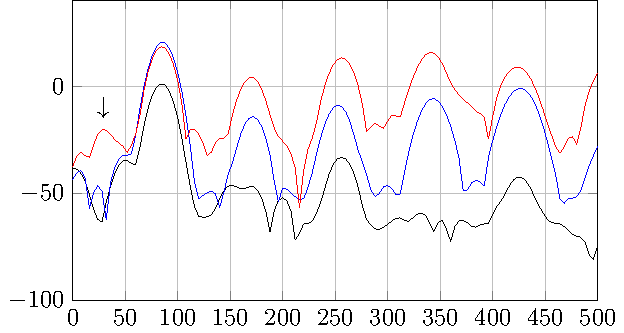
\includegraphics[width=0.6\textwidth]{FFT_hit}
%\end{figure}
%\begin{itemize}
%\item Sort: 0.005 Watt (81 dB SPL)
%\item Blå:  22 Watt (100 dB SPL)
%\item Rød:  294 Watt (105 dB SPL)
%
%\end{itemize}
%\end{frame}
%
%
%\subsection{Problemerne}
%\begin{frame}{Feedback system}{Problemerne}
%Følgende problemer ved feedback systemet:
%\begin{itemize}
%\item For dårlige sensorer
%\begin{itemize}
%\item Ikke præcise
%\item For meget støj
%\item For dyrer 
%\item Fejlmålinger
%\end{itemize}
%\item Ingen tendenser at spotte indtil et slag ramte = for sent
%\begin{itemize}
%\item Feedback tager for lang tid
%\end{itemize}
%\item Upraktisk at måle harmoniske toner 
%\begin{itemize}
%\item Ingen superpositions muligheder
%\item Fasen på signalerne passer ikke nødvendigvis
%\end{itemize}
%\end{itemize}
%\end{frame}
%
%%%%%%%%%%%%%%%%%
%
%\section{Feedforward system}
%
%\begin{frame}{Feedforward system}{Konceptet}
%
%\begin{figure}
%\centering
%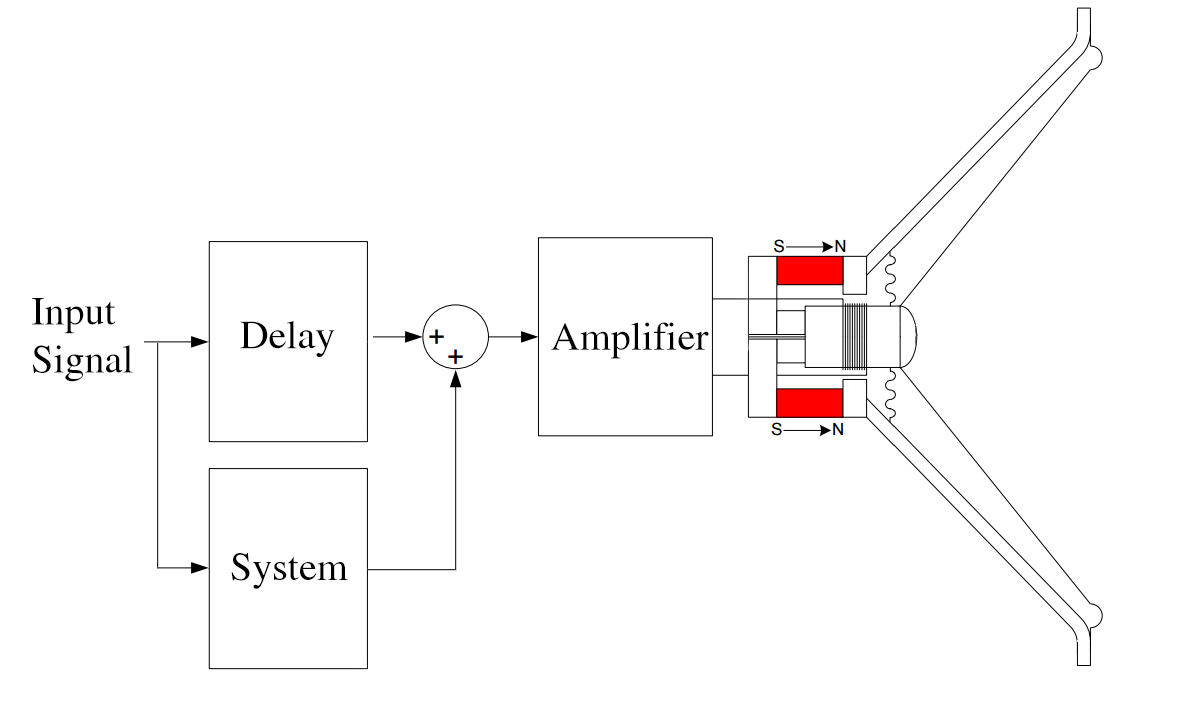
\includegraphics[width=0.9\textwidth]{Feedforward_Acc2}
%\end{figure}
%
%\end{frame}
%
%\begin{frame}{Feedforward system}{Overview}
%
%\begin{columns}
%  \begin{column}{0.70\textwidth}
%\begin{figure}
%\centering
%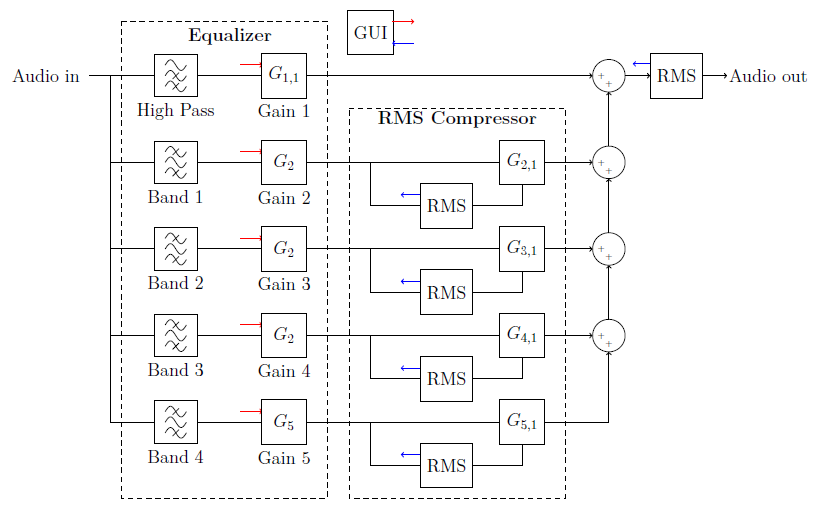
\includegraphics[width=0.85\textwidth]{Mainsystemoverview}
%\end{figure}
%  \end{column}
%  \begin{column}{0.30\textwidth}
%  \textbf{Systemet Overordnet}
%\begin{itemize}
%\item Grafisk Equalizer
%\item 4 Bånd i Bassen
%\begin{enumerate}
%\item 0   -   66 Hz
%\item 66  -  132 Hz
%\item 132 -  265 Hz
%\item 265 -  530 Hz
%\end{enumerate}
%\item RMS kompressor i 4 bånd
%\item RMS/Peak Limiter
%\item GUI til løbende justering
%\end{itemize}
%  \end{column}
%\end{columns}
%\end{frame}
%
%\subsection{Design Overvejelser}
%\begin{frame}{Feedforward system}{Design Overvejelser}
%\begin{columns}[t]
%  \begin{column}{0.50\textwidth}
%\textbf{Systemet skal:}
%\begin{itemize}
%\item Fungere ved lave frekvenser
%\item Have bånd til at måle frekvensområder
%\item Lineær fase
%\end{itemize}
%  \end{column}
%  \begin{column}{0.50\textwidth}
%  \textbf{Opnåes ved:}
%\begin{itemize}
%\item Realiseres som multi-rate
%\item Spektral subtraktion til at lave båndpas
%\item Opbygges af FIR filter
%\end{itemize}
%  \end{column}
%\end{columns}
%\vspace{5mm}
%\begin{block}{Overordnet set:}
%\begin{itemize}
%\item Downsampling til center frekvens på 3 kHz ved et 50-tap FIR filter
%\item x2 Downsampling 7 gange (x4,x8,x16,x32,x64)
%\item Indivudel kompressor i fire nederste bånd
%\end{itemize}
%\end{block}
%\end{frame}
%
%
%
%
%\subsection{Overordnet system}
%\begin{frame}{Feedforward system}{Systemet}
%
%\begin{columns}
%  \begin{column}{0.75\textwidth}
%\begin{figure}
%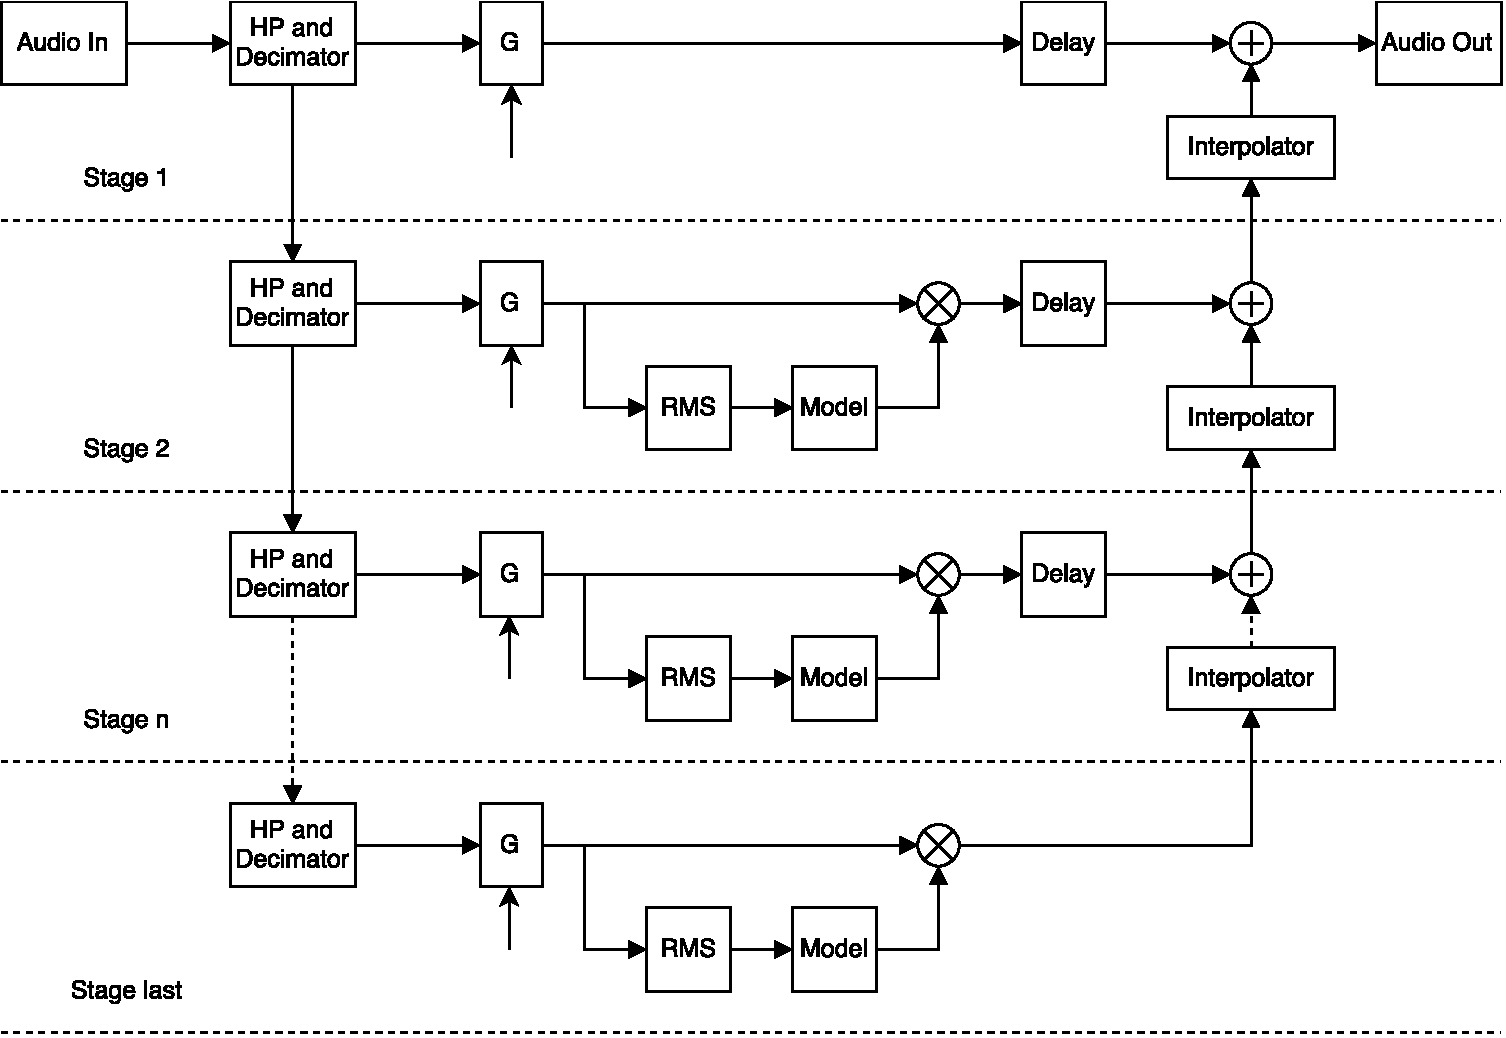
\includegraphics[width=\textwidth]{designRealBlock1}
%\end{figure}
%  \end{column}
%
%  \begin{column}{0.25\textwidth}
%  \textbf{Flow gennem system:}
%     \begin{enumerate}
%        \item Sample
%        \item Decimate
%        \item Spektral inversion
%        \item Påfør gain
%        \item Mål RMS
%        \item Påfør dæmpning
%        \item Interpolate
%        \item Summation
%     \end{enumerate}
%  \end{column}
%\end{columns}
%\end{frame}
%
%
%
%\subsection{Decimation}
%\begin{frame}{Feedforward system}{Decimator}
%
%\begin{columns}
%  \begin{column}{0.4\textwidth}
%\begin{figure}
%\centering
%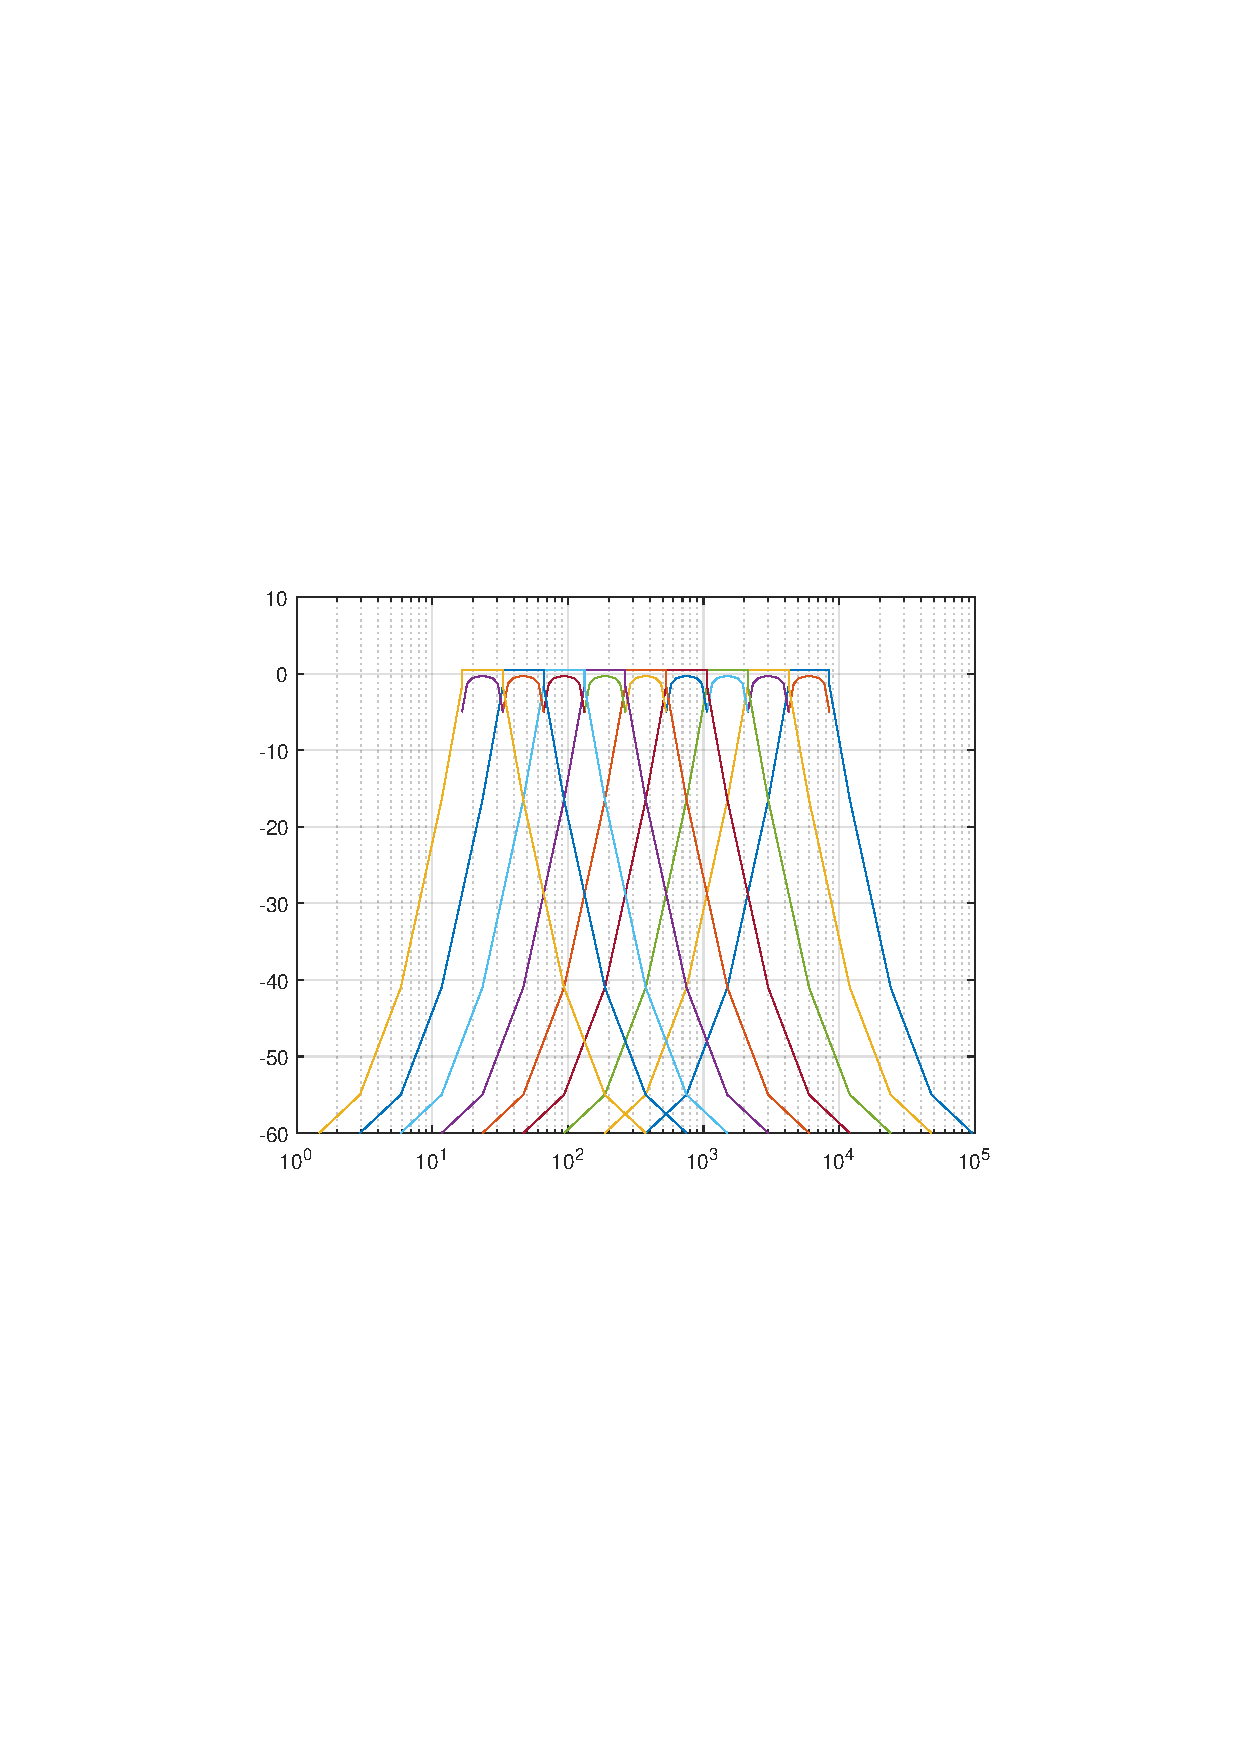
\includegraphics[width=\textwidth]{Bands}
%\end{figure}
%  \end{column}
%
%  \begin{column}{0.6\textwidth}
%\begin{itemize}
%\item 1 lavpas filter til båndpas
%\begin{itemize}
%\item Spektral subtraktion
%\end{itemize}
%\item 50. orden FIR
%\item Overholder IEC 6964 - Class 2 
%\end{itemize}
%\begin{figure}
%\centering
%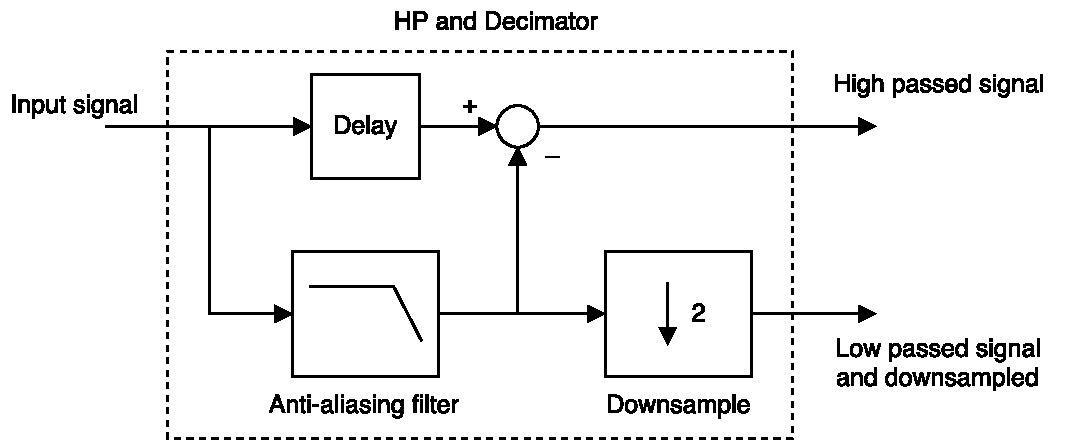
\includegraphics[width=\textwidth]{designRealDecimator}
%\end{figure}
%  \end{column}
%\end{columns}
%\end{frame}
%%%%%%%%%%%%%%%%%
%
%
%
%\subsection{RMS Compressor}
%\begin{frame}{Feedforward system}{RMS Compressor}
%
%\begin{columns}
%  \begin{column}{0.5\textwidth}
%\begin{figure}
%\centering
%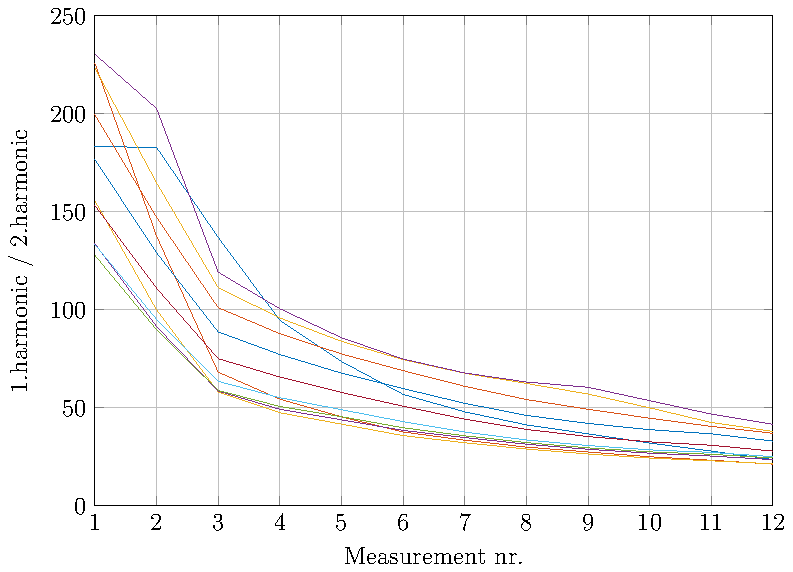
\includegraphics[width=0.7\textwidth]{comp_mic12All}
%\end{figure}
%\vspace{-5mm}
%\begin{figure}
%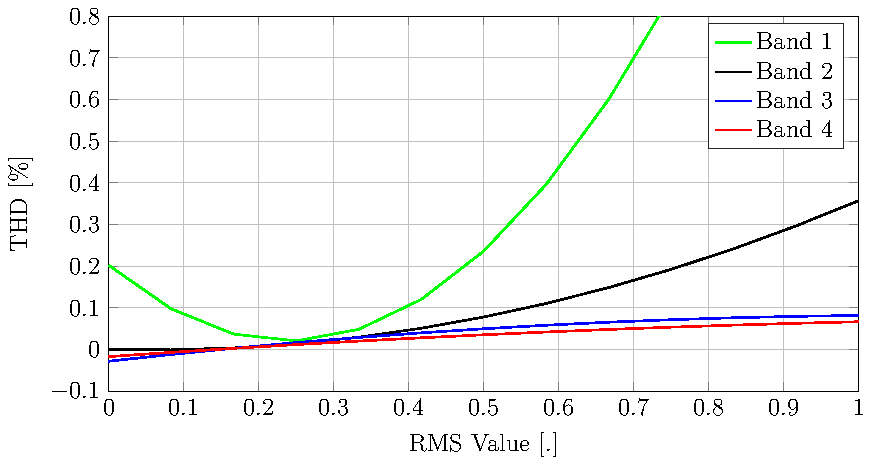
\includegraphics[width=0.8\textwidth]{BandModelCombine}
%\end{figure}
%  \end{column}
%  \begin{column}{0.5\textwidth}
%\begin{itemize}
%\item Dæmpning på op til 60 dB
%\item Opløsning på 1024 Steps
%\item Udskiftelig modeller
%\end{itemize}
%\begin{figure}
%\centering
%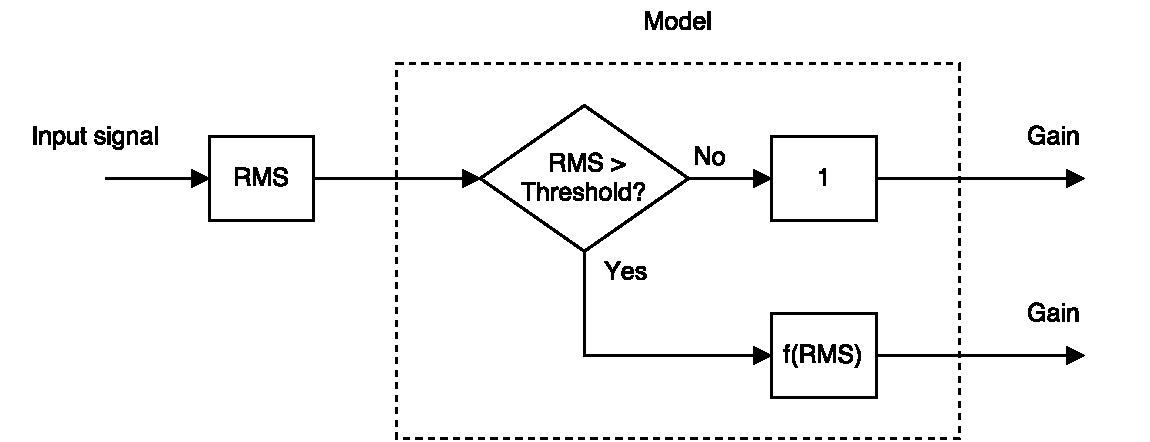
\includegraphics[width=\textwidth]{designRealRMS}
%\end{figure}
%  \end{column}
%\end{columns}
%
%\end{frame}
%
%
%
%
%\subsection{Interpolation}
%\begin{frame}{Feedforward system}{Interpolation}
%
%\begin{columns}
%  \begin{column}{0.4\textwidth}
%%\begin{figure}
%%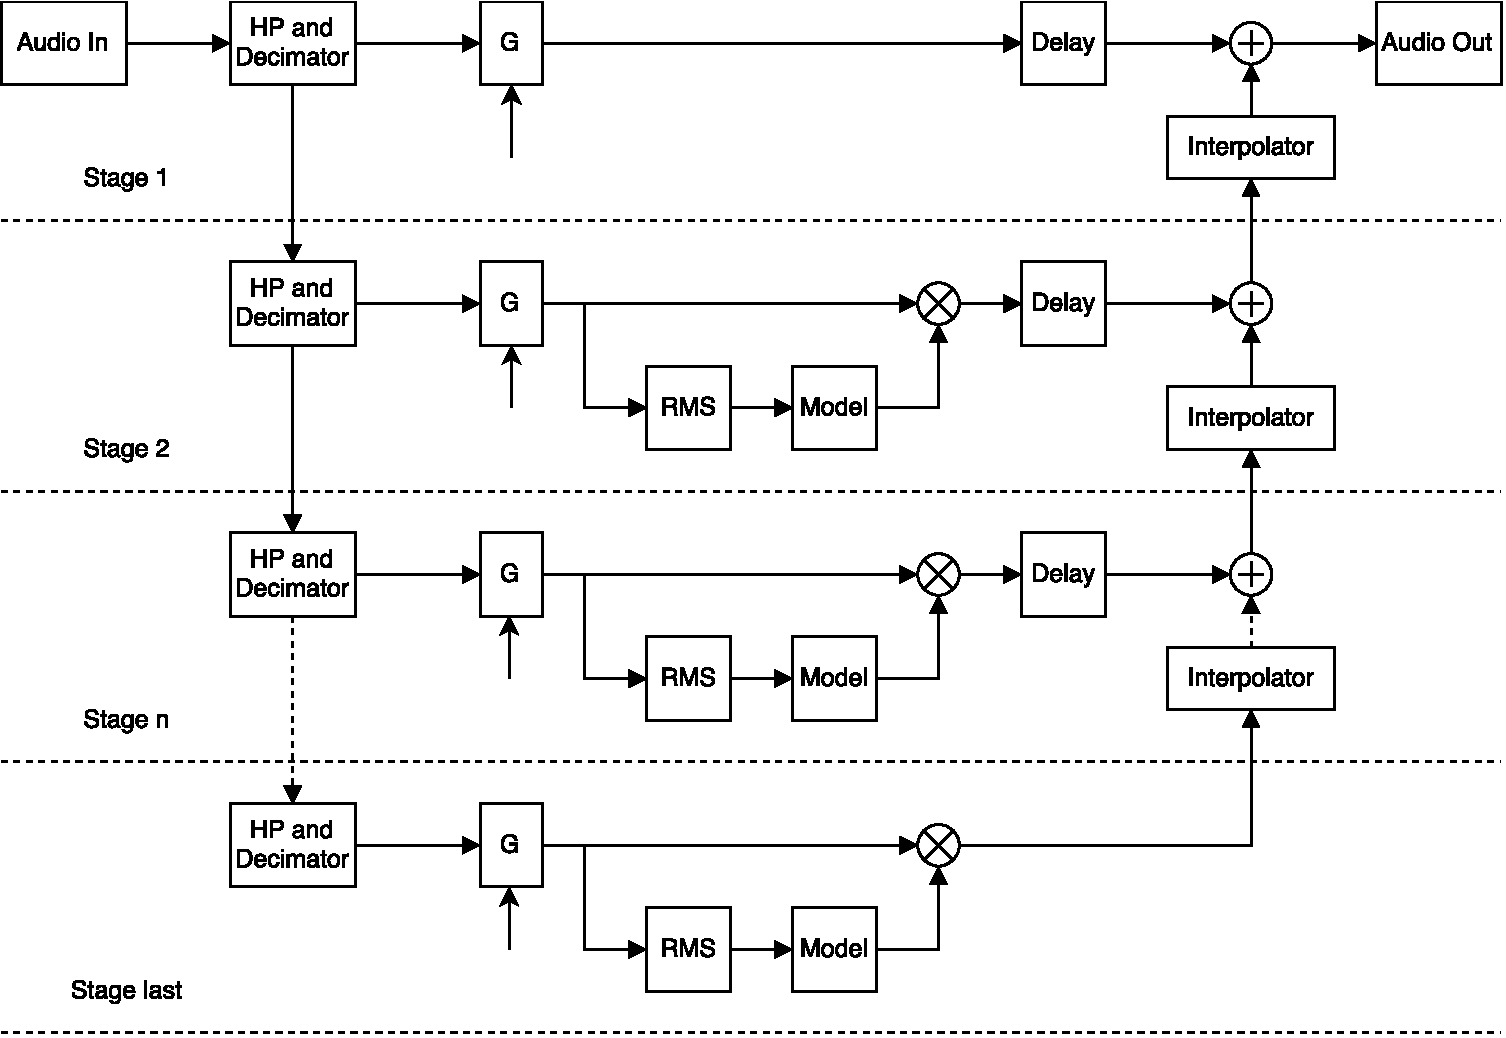
\includegraphics[width=0.9\textwidth]{designRealBlock1}
%%\end{figure}
%\begin{itemize}
%\item Zero-padding
%\item 48. Orden FIR
%\item Gain x2
%\end{itemize}
%  \end{column}
%
%  \begin{column}{0.6\textwidth}
%\begin{figure}
%\centering
%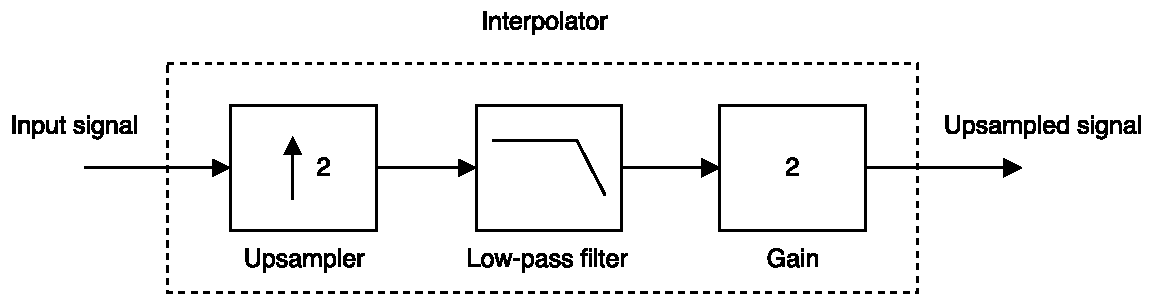
\includegraphics[width=\textwidth]{designRealInterpolator}
%\end{figure}
%  \end{column}
%\end{columns}
%
%\end{frame}
%
%
%
%\subsection{Simulering}
%\begin{frame}{Feedforward system}{Simulering}
%
%\begin{center}
%Simulering i MATLAB
%\end{center}
%
%\end{frame}
%
%\subsection{Opsumering}
%\begin{frame}{Feedforward system}{Opsumering}
%
%\begin{columns}[t]
%\begin{column}{0.40\textwidth}
%\textbf{Decimation/Interpolation:}
%\begin{itemize}
%\item Få instruktioner / Lav orden
%\item Billige FIR filter
%\item Mulighed for mere optimering
%\end{itemize}
%  \end{column}
%  \begin{column}{0.3\textwidth}
%\textbf{RMS Compressor:}
%\begin{itemize}
%\item Fleksible modeller
%\item Minimere hård limitering
%\item Fungere som både Peak og RMS
%\end{itemize}
%  \end{column}
%    \begin{column}{0.3\textwidth}
%\textbf{Overall:}
%\begin{itemize}
%\item Ingen støj
%\item Flat respons (+/- 1 dB)
%\end{itemize}
%  \end{column}
%\end{columns}
%
%\begin{block}{Kan Realiseres med:}
%\begin{itemize}
%\item Mulighed for 32-bit og 192 kHz
%\begin{itemize}
%\item Kun en ALU brugt
%\item 192 kHz vil kræve (x128,x256)
%\end{itemize}
%\end{itemize}
%\end{block}
%\vspace{-3mm}
%\begin{block}{Er Realiseret med:}
%\begin{itemize}
%\item Ca. 800 instruktioner.
%\item 16-bit og 48 kHz
%\item Peak limiter, RMS compressor og grafisk equalizer.
%\end{itemize}
%\end{block}
%
%\end{frame}
%
%
%\section{Demonstration}
%\begin{frame}{Feedforward system}{DEMO}
%
%\begin{center}
%DEMO\\
%\textit{Med forbehold}
%\end{center}
%\end{frame}
%
%\section{Spørgsmål og Evt.}
%% contact information
%\begin{frame}{Spørgsmål og Evt.}
%  \begin{center}
%Spørgsmål og Evt.
%  \end{center}
%\end{frame}

\section{Opbygning}
\begin{frame}{Opbygning}{Undertitel}
	Something new and awesome
\end{frame}

\subsection{Multi-Rate/stage}
\begin{frame}{Opbygning}{Multi-Rate/stage}
	Something new and awesome
\end{frame}


\subsection{Filter Design}
\begin{frame}{Opbygning}{Filter Design}
	Something new and awesome
\end{frame}

\subsection{Limiter}
\begin{frame}{Opbygning}{Limiter}
	Something new and awesome
\end{frame}

\section{Resultat \& Konklusion}
\begin{frame}{Resultat \& Konklusion}{...}
	Something new and awesome
\end{frame}



%\section{Introduktion}
%% motivation for creating this theme
%\begin{frame}{Introduktion}{}
%  Målet med dette projekt er at:
%  \begin{itemize}
%    \item Beskytte bas enhederne
%    \begin{itemize}
%    \item Begrænse slag mod bagpladen
%\end{itemize}
%\item Minimal komprimering/limitering       
%  \end{itemize}
%  \vspace{5mm}
%  Samtidigt med at følgende krav kunne realiseres:
%  \begin{itemize}
%  	\item Mindre end 1024 Instruktioner pr. sample
%  	\item Mulighed for sampling rate på 96 kHz
%  	\item Mulighed for at køre med 24-Bit
%  \end{itemize}
%\end{frame}
%%%%%%%%%%%%%%%%%
%
%\section{Feedback system}
%% the license
%\begin{frame}{Feedback system}{Første antagelse}
%\begin{figure}[t]
%\centering
%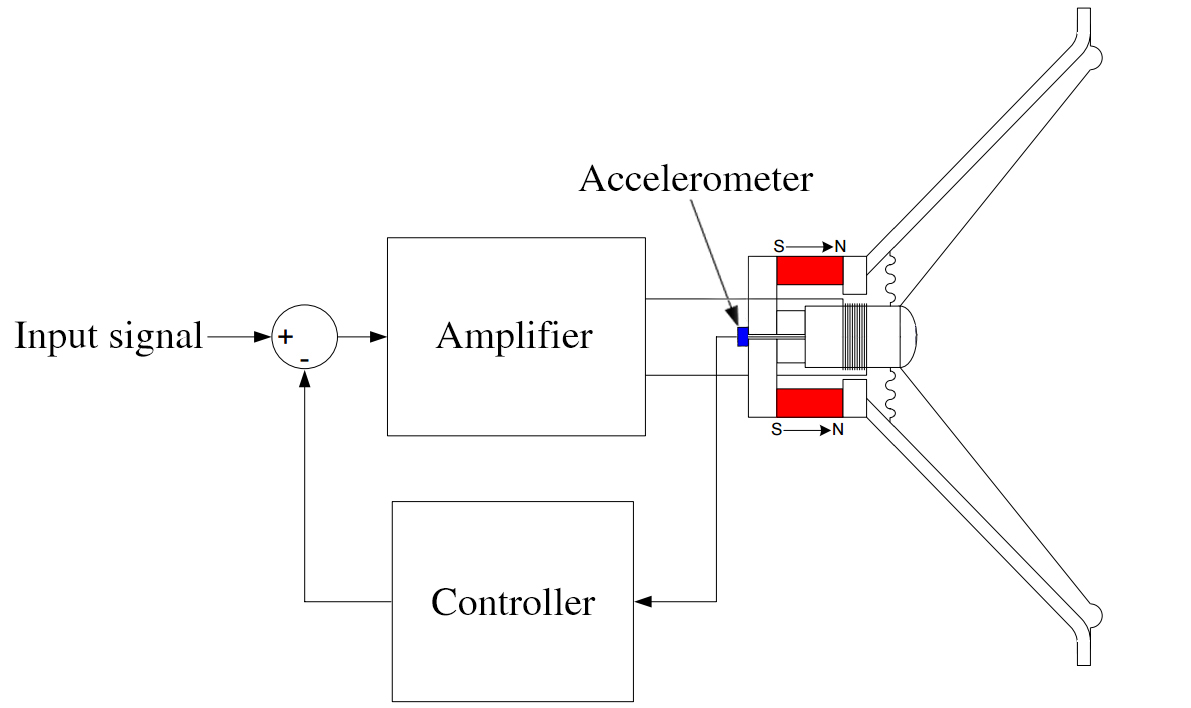
\includegraphics[width=0.75\textwidth]{Feedback_Acc2}
%\end{figure}
%\end{frame}
%
%\subsection{Analyse}
%\begin{frame}{Feedback system}{Analyse}
%Lineært sweep fra 2400 til 0 Hz
%\begin{figure}
%\centering
%\begin{subfigure}[t]{0.45\textwidth}
%\centering
%%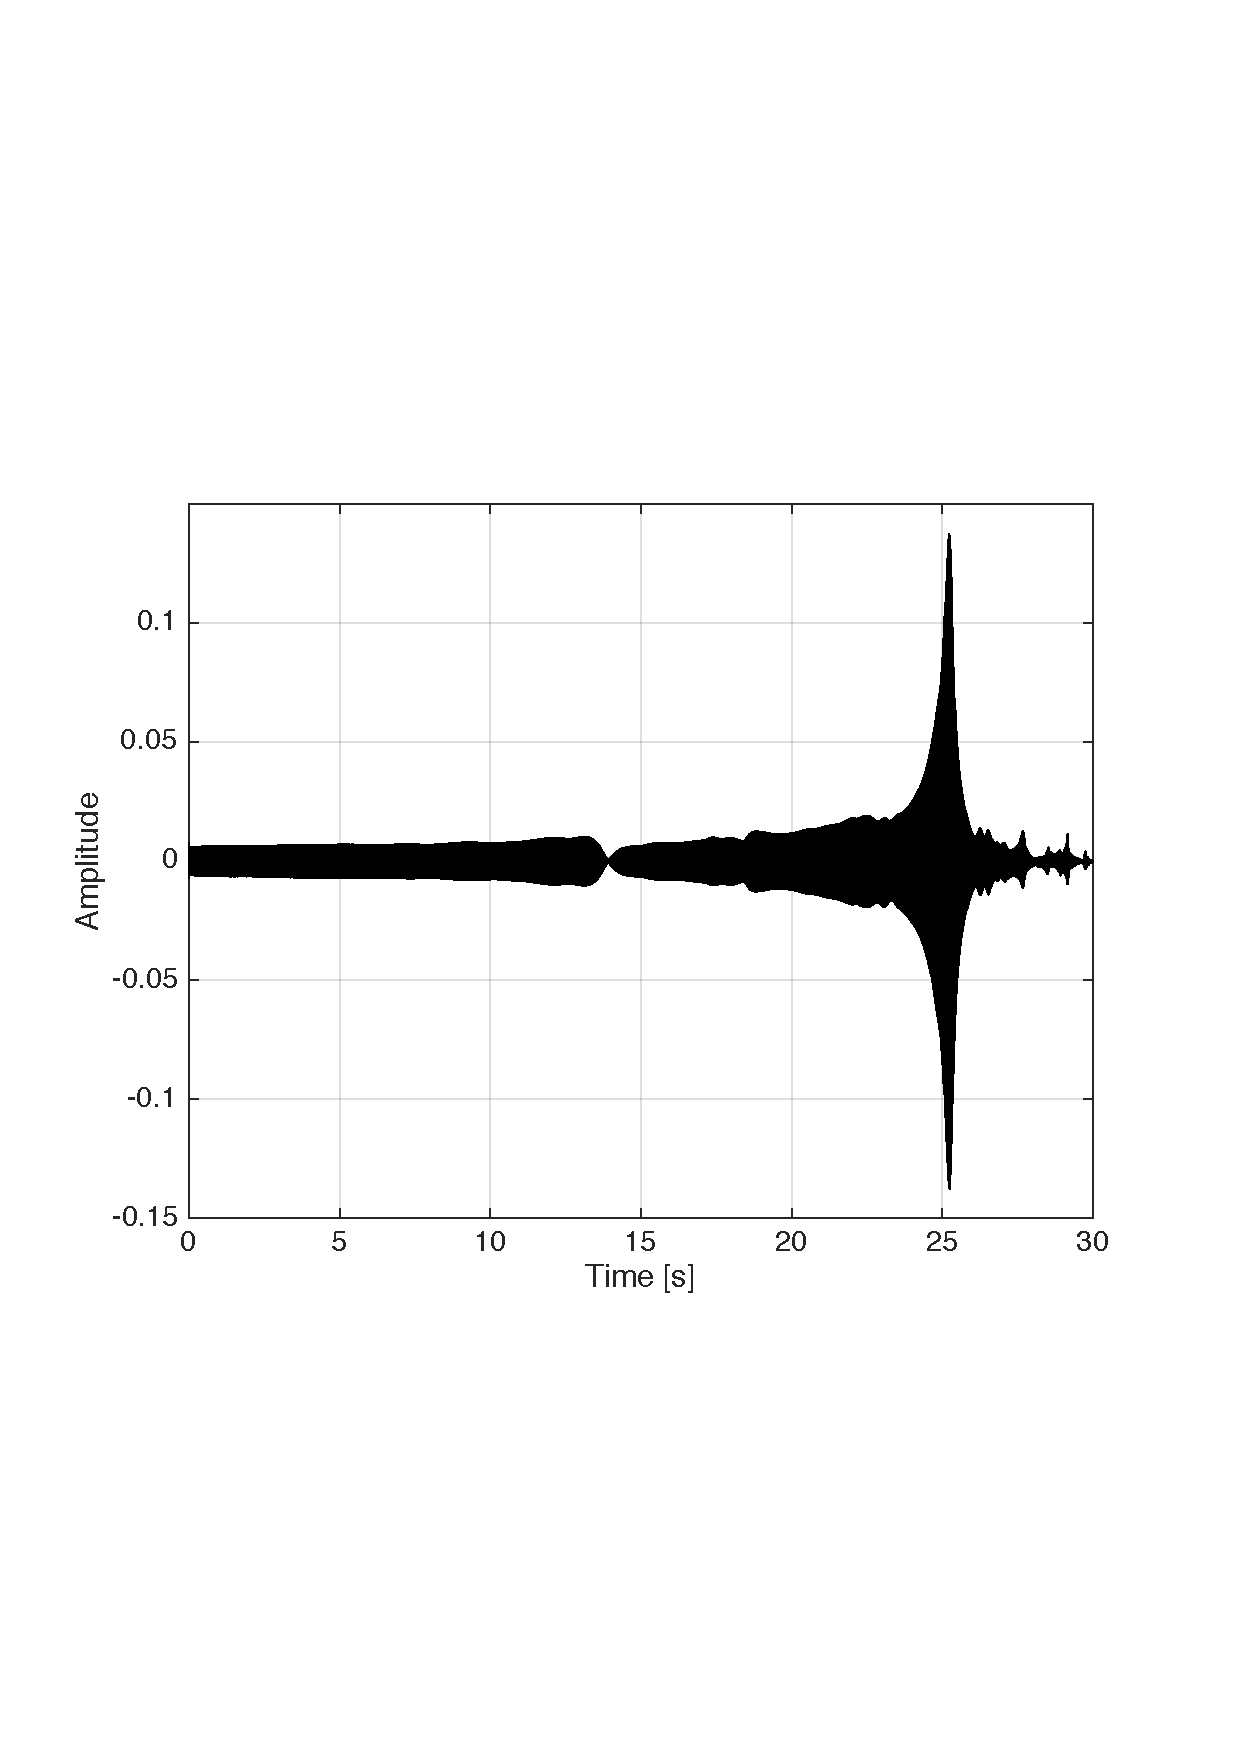
\includegraphics[width=\textwidth]{raw_driver10}
%% This file was created by matlab2tikz.
%
%The latest updates can be retrieved from
%  http://www.mathworks.com/matlabcentral/fileexchange/22022-matlab2tikz-matlab2tikz
%where you can also make suggestions and rate matlab2tikz.
%
\begin{tikzpicture}

\begin{axis}[%
width=5.521in,
height=2in,
at={(0.758in,0.481in)},
xmin=0,
xmax=30,
xmajorgrids,
ymin=-0.15,
ymax=0.15,
ymajorgrids,
axis background/.style={fill=white}
]
\addplot[fill=black,draw=black,forget plot] plot table[row sep=crcr]{%
2.08333333333333e-05	0.0119891166687012\\
0.0425739952718676	0.0120701789855957\\
0.0851271572104019	0.0120600461959839\\
0.127680319148936	0.0121411085128784\\
0.17023348108747	0.0122112035751343\\
0.212786643026005	0.0122820138931274\\
0.255339804964539	0.0123153924942017\\
0.297892966903073	0.0123672485351563\\
0.340446128841608	0.0123822689056396\\
0.382999290780142	0.0124343633651733\\
0.425552452718676	0.012420654296875\\
0.46810561465721	0.0124455690383911\\
0.510658776595745	0.0124385356903076\\
0.553211938534279	0.0124293565750122\\
0.595765100472813	0.0124131441116333\\
0.638318262411347	0.0123996734619141\\
0.680871424349882	0.0123659372329712\\
0.723424586288416	0.0123772621154785\\
0.76597774822695	0.0123530626296997\\
0.808530910165485	0.0123927593231201\\
0.851084072104019	0.0123993158340454\\
0.893637234042553	0.0123468637466431\\
0.936190395981088	0.0123317241668701\\
0.978743557919622	0.0123351812362671\\
1.02129671985816	0.0123213529586792\\
1.06384988179669	0.012315034866333\\
1.10640304373522	0.0123295783996582\\
1.14895620567376	0.0123213529586792\\
1.19150936761229	0.012312650680542\\
1.23406252955083	0.0123451948165894\\
1.27661569148936	0.0123229026794434\\
1.3191688534279	0.0123435258865356\\
1.36172201536643	0.0123484134674072\\
1.40427517730496	0.0123796463012695\\
1.4468283392435	0.0123721361160278\\
1.48938150118203	0.0123879909515381\\
1.53193466312057	0.012427806854248\\
1.5744878250591	0.0124756097793579\\
1.61704098699764	0.012513279914856\\
1.65959414893617	0.0124995708465576\\
1.7021473108747	0.0125466585159302\\
1.74470047281324	0.012596607208252\\
1.78725363475177	0.0126116275787354\\
1.82980679669031	0.0126550197601318\\
1.87235995862884	0.012694239616394\\
1.91491312056738	0.0127073526382446\\
1.95746628250591	0.0127198696136475\\
2.00001944444444	0.0127586126327515\\
2.04257260638298	0.0127676725387573\\
2.08512576832151	0.012792706489563\\
2.12767893026005	0.0128316879272461\\
2.17023209219858	0.0128744840621948\\
2.21278525413712	0.0128858089447021\\
2.25533841607565	0.0128728151321411\\
2.29789157801418	0.0128904581069946\\
2.34044473995272	0.012937068939209\\
2.38299790189125	0.0129625797271729\\
2.42555106382979	0.0129508972167969\\
2.46810422576832	0.0129650831222534\\
2.51065738770686	0.0130186080932617\\
2.55321054964539	0.0130044221878052\\
2.59576371158392	0.0130490064620972\\
2.63831687352246	0.0130782127380371\\
2.68087003546099	0.0130912065505981\\
2.72342319739953	0.0131031274795532\\
2.76597635933806	0.0131406784057617\\
2.8085295212766	0.0131857395172119\\
2.85108268321513	0.0132355690002441\\
2.89363584515366	0.0132455825805664\\
2.9361890070922	0.0132309198379517\\
2.97874216903073	0.013269305229187\\
3.02129533096927	0.0133043527603149\\
3.0638484929078	0.013329029083252\\
3.10640165484634	0.0133227109909058\\
3.14895481678487	0.0133368968963623\\
3.1915079787234	0.0133442878723145\\
3.23406114066194	0.0133599042892456\\
3.27661430260047	0.0133839845657349\\
3.31916746453901	0.0133798122406006\\
3.36172062647754	0.0133849382400513\\
3.40427378841608	0.0134093761444092\\
3.44682695035461	0.013446569442749\\
3.48938011229314	0.0134661197662354\\
3.53193327423168	0.0134836435317993\\
3.57448643617021	0.013521671295166\\
3.61703959810875	0.0135370492935181\\
3.65959276004728	0.0135470628738403\\
3.70214592198582	0.0135759115219116\\
3.74469908392435	0.0136080980300903\\
3.78725224586288	0.0136371850967407\\
3.82980540780142	0.0136731863021851\\
3.87235856973995	0.0137186050415039\\
3.91491173167849	0.0137549638748169\\
3.95746489361702	0.0137441158294678\\
4.00001805555556	0.0138174295425415\\
4.04257121749409	0.013864278793335\\
4.08512437943262	0.0139147043228149\\
4.12767754137116	0.0139368772506714\\
4.17023070330969	0.0140061378479004\\
4.21278386524823	0.0140299797058105\\
4.25533702718676	0.0140790939331055\\
4.29789018912529	0.0141112804412842\\
4.34044335106383	0.0141588449478149\\
4.38299651300236	0.0141901969909668\\
4.4255496749409	0.0142172574996948\\
4.46810283687943	0.0142718553543091\\
4.51065599881797	0.0143095254898071\\
4.5532091607565	0.0143332481384277\\
4.59576232269503	0.0143661499023438\\
4.63831548463357	0.0144078731536865\\
4.6808686465721	0.0144317150115967\\
4.72342180851064	0.014464259147644\\
4.76597497044917	0.0144739151000977\\
4.80852813238771	0.0144917964935303\\
4.85108129432624	0.0145350694656372\\
4.89363445626477	0.0145490169525146\\
4.93618761820331	0.014581561088562\\
4.97874078014184	0.0145977735519409\\
5.02129394208038	0.0146069526672363\\
5.06384710401891	0.0146232843399048\\
5.10640026595745	0.0146393775939941\\
5.14895342789598	0.0146942138671875\\
5.19150658983452	0.0146994590759277\\
5.23405975177305	0.0147175788879395\\
5.27661291371158	0.0147092342376709\\
5.31916607565012	0.0147404670715332\\
5.36171923758865	0.0147354602813721\\
5.40427239952719	0.0147433280944824\\
5.44682556146572	0.0147520303726196\\
5.48937872340426	0.0147508382797241\\
5.53193188534279	0.0147504806518555\\
5.57448504728132	0.014761209487915\\
5.61703820921986	0.0147466659545898\\
5.65959137115839	0.0147426128387451\\
5.70214453309693	0.0147403478622437\\
5.74469769503546	0.0147124528884888\\
5.787250856974	0.0147058963775635\\
5.82980401891253	0.0147024393081665\\
5.87235718085106	0.0146327018737793\\
5.9149103427896	0.0146118402481079\\
5.95746350472813	0.0145947933197021\\
6.00001666666667	0.0145722627639771\\
6.0425698286052	0.0145455598831177\\
6.08512299054374	0.0144891738891602\\
6.12767615248227	0.0144437551498413\\
6.1702293144208	0.0144070386886597\\
6.21278247635934	0.014379620552063\\
6.25533563829787	0.0143579244613647\\
6.29788880023641	0.0142805576324463\\
6.34044196217494	0.0142168998718262\\
6.38299512411347	0.014191746711731\\
6.42554828605201	0.0140836238861084\\
6.46810144799054	0.0140348672866821\\
6.51065460992908	0.0139898061752319\\
6.55320777186761	0.0139384269714355\\
6.59576093380615	0.0138537883758545\\
6.63831409574468	0.0137983560562134\\
6.68086725768321	0.0137511491775513\\
6.72342041962175	0.0137094259262085\\
6.76597358156028	0.0136710405349731\\
6.80852674349882	0.0136563777923584\\
6.85107990543735	0.0136498212814331\\
6.89363306737589	0.0136363506317139\\
6.93618622931442	0.0136944055557251\\
6.97873939125296	0.0137603282928467\\
7.02129255319149	0.0138442516326904\\
7.06384571513002	0.0139046907424927\\
7.10639887706856	0.0139477252960205\\
7.14895203900709	0.014054536819458\\
7.19150520094563	0.0141353607177734\\
7.23405836288416	0.0142430067062378\\
7.27661152482269	0.0143053531646729\\
7.31916468676123	0.014385461807251\\
7.36171784869976	0.0145281553268433\\
7.4042710106383	0.0145792961120605\\
7.44682417257683	0.0146374702453613\\
7.48937733451537	0.014722466468811\\
7.5319304964539	0.0147558450698853\\
7.57448365839243	0.0148293972015381\\
7.61703682033097	0.0148519277572632\\
7.6595899822695	0.0148772001266479\\
7.70214314420804	0.0148836374282837\\
7.74469630614657	0.0149027109146118\\
7.78724946808511	0.0148898363113403\\
7.82980263002364	0.0149227380752563\\
7.87235579196217	0.0149306058883667\\
7.91490895390071	0.0149260759353638\\
7.95746211583924	0.0149365663528442\\
8.00001527777778	0.0149394273757935\\
8.04256843971631	0.0149445533752441\\
8.08512160165485	0.0149415731430054\\
8.12767476359338	0.0149654150009155\\
8.17022792553192	0.0149649381637573\\
8.21278108747045	0.014962911605835\\
8.25533424940898	0.0149157047271729\\
8.29788741134752	0.0148886442184448\\
8.34044057328605	0.0148481130599976\\
8.38299373522459	0.0147963762283325\\
8.42554689716312	0.0147671699523926\\
8.46810005910165	0.0147316455841064\\
8.51065322104019	0.0146907567977905\\
8.55320638297872	0.0146373510360718\\
8.59575954491726	0.0146878957748413\\
8.63831270685579	0.0146653652191162\\
8.68086586879433	0.0146582126617432\\
8.72341903073286	0.0146515369415283\\
8.76597219267139	0.0146892070770264\\
8.80852535460993	0.0147384405136108\\
8.85107851654846	0.0147976875305176\\
8.893631678487	0.0148004293441772\\
8.93618484042553	0.0149153470993042\\
8.97873800236407	0.0149699449539185\\
9.0212911643026	0.0150353908538818\\
9.06384432624114	0.0150772333145142\\
9.10639748817967	0.0151313543319702\\
9.1489506501182	0.0152260065078735\\
9.19150381205674	0.0153157711029053\\
9.23405697399527	0.015323281288147\\
9.27661013593381	0.0154021978378296\\
9.31916329787234	0.0154614448547363\\
9.36171645981088	0.0155340433120728\\
9.40426962174941	0.015607476234436\\
9.44682278368794	0.015711784362793\\
9.48937594562648	0.0157406330108643\\
9.53192910756501	0.0158414840698242\\
9.57448226950355	0.0159074068069458\\
9.61703543144208	0.0159391164779663\\
9.65958859338062	0.0160180330276489\\
9.70214175531915	0.0160245895385742\\
9.74469491725768	0.0160360336303711\\
9.78724807919622	0.01607346534729\\
9.82980124113475	0.0160551071166992\\
9.87235440307329	0.0160226821899414\\
9.91490756501182	0.0159975290298462\\
9.95746072695036	0.0159332752227783\\
10.0000138888889	0.0159041881561279\\
10.0425670508274	0.0158710479736328\\
10.085120212766	0.0158164501190186\\
10.1276733747045	0.0158092975616455\\
10.170226536643	0.0157977342605591\\
10.2127796985816	0.0158299207687378\\
10.2553328605201	0.0159136056900024\\
10.2978860224586	0.0159791707992554\\
10.3404391843972	0.016069769859314\\
10.3829923463357	0.0161577463150024\\
10.4255455082742	0.0162630081176758\\
10.4680986702128	0.0163758993148804\\
10.5106518321513	0.0164648294448853\\
10.5532049940898	0.0165594816207886\\
10.5957581560284	0.0166622400283813\\
10.6383113179669	0.016768217086792\\
10.6808644799054	0.0168865919113159\\
10.723417641844	0.0169931650161743\\
10.7659708037825	0.0171152353286743\\
10.808523965721	0.0171926021575928\\
10.8510771276596	0.017282247543335\\
10.8936302895981	0.0174212455749512\\
10.9361834515366	0.0175200700759888\\
10.9787366134752	0.0176385641098022\\
11.0212897754137	0.0177961587905884\\
11.0638429373522	0.0178617238998413\\
11.1063960992908	0.0179822444915771\\
11.1489492612293	0.0180516242980957\\
11.1915024231678	0.0181763172149658\\
11.2340555851064	0.0183032751083374\\
11.2766087470449	0.0184470415115356\\
11.3191619089835	0.0185744762420654\\
11.361715070922	0.0186715126037598\\
11.4042682328605	0.0187947750091553\\
11.4468213947991	0.0189191102981567\\
11.4893745567376	0.0189660787582397\\
11.5319277186761	0.0190688371658325\\
11.5744808806147	0.019160270690918\\
11.6170340425532	0.0192372798919678\\
11.6595872044917	0.0193090438842773\\
11.7021403664303	0.019400954246521\\
11.7446935283688	0.0195177793502808\\
11.7872466903073	0.0195590257644653\\
11.8297998522459	0.0196257829666138\\
11.8723530141844	0.0197001695632935\\
11.9149061761229	0.0197663307189941\\
11.9574593380615	0.0198649168014526\\
12.0000125	0.0199562311172485\\
12.0425656619385	0.0200393199920654\\
12.0851188238771	0.0201531648635864\\
12.1276719858156	0.0202683210372925\\
12.1702251477541	0.0203834772109985\\
12.2127783096927	0.0205181837081909\\
12.2553314716312	0.0206431150436401\\
12.2978846335697	0.020803689956665\\
12.3404377955083	0.0209430456161499\\
12.3829909574468	0.0210655927658081\\
12.4255441193853	0.0211613178253174\\
12.4680972813239	0.0213009119033813\\
12.5106504432624	0.0214111804962158\\
12.5532036052009	0.0215167999267578\\
12.5957567671395	0.0215667486190796\\
12.638309929078	0.0216765403747559\\
12.6808630910165	0.0217441320419312\\
12.7234162529551	0.0217874050140381\\
12.7659694148936	0.0218304395675659\\
12.8085225768322	0.0218579769134521\\
12.8510757387707	0.0218334197998047\\
12.8936289007092	0.0218534469604492\\
12.9361820626478	0.0217874050140381\\
12.9787352245863	0.0216927528381348\\
13.0212883865248	0.021544337272644\\
13.0638415484634	0.021371603012085\\
13.1063947104019	0.0211578607559204\\
13.1489478723404	0.0209262371063232\\
13.191501034279	0.0206685066223145\\
13.2340541962175	0.0203869342803955\\
13.276607358156	0.0200080871582031\\
13.3191605200946	0.019722580909729\\
13.3617136820331	0.0194058418273926\\
13.4042668439716	0.0190954208374023\\
13.4468200059102	0.0187587738037109\\
13.4893731678487	0.0184516906738281\\
13.5319263297872	0.0181584358215332\\
13.5744794917258	0.0178221464157104\\
13.6170326536643	0.0174729824066162\\
13.6595858156028	0.0171077251434326\\
13.7021389775414	0.016639232635498\\
13.7446921394799	0.0161151885986328\\
13.7872453014184	0.0154547691345215\\
13.829798463357	0.0146360397338867\\
13.8723516252955	0.0137324333190918\\
13.914904787234	0.0126259326934814\\
13.9574579491726	0.0113997459411621\\
14.0000111111111	0.0100481510162354\\
14.0425642730496	0.00874054431915283\\
14.0851174349882	0.00763881206512451\\
14.1276705969267	0.00698995590209961\\
14.1702237588652	0.00721240043640137\\
14.2127769208038	0.0078728199005127\\
14.2553300827423	0.00864839553833008\\
14.2978832446809	0.00943124294281006\\
14.3404364066194	0.010124683380127\\
14.3829895685579	0.0107450485229492\\
14.4255427304965	0.0112762451171875\\
14.468095892435	0.0117151737213135\\
14.5106490543735	0.0120129585266113\\
14.5532022163121	0.0122971534729004\\
14.5957553782506	0.0124787092208862\\
14.6383085401891	0.0126643180847168\\
14.6808617021277	0.0127860307693481\\
14.7234148640662	0.0129104852676392\\
14.7659680260047	0.013019323348999\\
14.8085211879433	0.0130923986434937\\
14.8510743498818	0.0131598711013794\\
14.8936275118203	0.0132442712783813\\
14.9361806737589	0.0132671594619751\\
14.9787338356974	0.0133401155471802\\
15.0212869976359	0.0133960247039795\\
15.0638401595745	0.0134508609771729\\
15.106393321513	0.0134987831115723\\
15.1489464834515	0.0135847330093384\\
15.1914996453901	0.0137389898300171\\
15.2340528073286	0.0139615535736084\\
15.2766059692671	0.0141968727111816\\
15.3191591312057	0.0144667625427246\\
15.3617122931442	0.0147184133529663\\
15.4042654550827	0.0149639844894409\\
15.4468186170213	0.0151892900466919\\
15.4893717789598	0.0153195858001709\\
15.5319249408983	0.0154467821121216\\
15.5744781028369	0.0155524015426636\\
15.6170312647754	0.0156270265579224\\
15.6595844267139	0.0157109498977661\\
15.7021375886525	0.0157914161682129\\
15.744690750591	0.0158919095993042\\
15.7872439125296	0.0159846544265747\\
15.8297970744681	0.0160763263702393\\
15.8723502364066	0.0161715745925903\\
15.9149033983452	0.0162194967269897\\
15.9574565602837	0.0162959098815918\\
16.0000097222222	0.0163196325302124\\
16.0425628841608	0.0163333415985107\\
16.0851160460993	0.0164139270782471\\
16.1276692080378	0.0164852142333984\\
16.1702223699764	0.016596794128418\\
16.2127755319149	0.0167173147201538\\
16.2553286938534	0.016867995262146\\
16.297881855792	0.0169942378997803\\
16.3404350177305	0.0171358585357666\\
16.382988179669	0.017247200012207\\
16.4255413416076	0.0173672437667847\\
16.4680945035461	0.0174224376678467\\
16.5106476654846	0.0174494981765747\\
16.5532008274232	0.0174441337585449\\
16.5957539893617	0.0174261331558228\\
16.6383071513002	0.0173689126968384\\
16.6808603132388	0.017351508140564\\
16.7234134751773	0.0173255205154419\\
16.7659666371158	0.0173234939575195\\
16.8085197990544	0.0173735618591309\\
16.8510729609929	0.0174065828323364\\
16.8936261229314	0.0174649953842163\\
16.93617928487	0.017520546913147\\
16.9787324468085	0.0175772905349731\\
17.021285608747	0.017709493637085\\
17.0638387706856	0.017842173576355\\
17.1063919326241	0.0179907083511353\\
17.1489450945626	0.0182030200958252\\
17.1914982565012	0.0184568166732788\\
17.2340514184397	0.0187783241271973\\
17.2766045803783	0.0191693305969238\\
17.3191577423168	0.0196816921234131\\
17.3617109042553	0.0201215744018555\\
17.4042640661939	0.0205991268157959\\
17.4468172281324	0.0209838151931763\\
17.4893703900709	0.0212384462356567\\
17.5319235520095	0.0214720964431763\\
17.574476713948	0.0217106342315674\\
17.6170298758865	0.0218876600265503\\
17.6595830378251	0.0220842361450195\\
17.7021361997636	0.0222510099411011\\
17.7446893617021	0.0224254131317139\\
17.7872425236407	0.0225731134414673\\
17.8297956855792	0.0227036476135254\\
17.8723488475177	0.0228030681610107\\
17.9149020094563	0.0228255987167358\\
17.9574551713948	0.0227867364883423\\
18.0000083333333	0.0226969718933105\\
18.0425614952719	0.0225468873977661\\
18.0851146572104	0.022442102432251\\
18.1276678191489	0.0224337577819824\\
18.1702209810875	0.0225523710250854\\
18.212774143026	0.0226941108703613\\
18.2553273049645	0.0227112770080566\\
18.2978804669031	0.0226702690124512\\
18.3404336288416	0.0225247144699097\\
18.3829867907801	0.022191047668457\\
18.4255399527187	0.0216506719589233\\
18.4680931146572	0.0210781097412109\\
18.5106462765957	0.0205855369567871\\
18.5531994385343	0.0202169418334961\\
18.5957526004728	0.0198911428451538\\
18.6383057624113	0.0195983648300171\\
18.6808589243499	0.0192761421203613\\
18.7234120862884	0.0189481973648071\\
18.765965248227	0.0187180042266846\\
18.8085184101655	0.0185004472732544\\
18.851071572104	0.0183453559875488\\
18.8936247340426	0.0182894468307495\\
18.9361778959811	0.018202543258667\\
18.9787310579196	0.0181392431259155\\
19.0212842198582	0.018133282661438\\
19.0638373817967	0.0181257724761963\\
19.1063905437352	0.0182130336761475\\
19.1489437056738	0.0184046030044556\\
19.1914968676123	0.0186821222305298\\
19.2340500295508	0.0190776586532593\\
19.2766031914894	0.0195093154907227\\
19.3191563534279	0.0199741125106812\\
19.3617095153664	0.020482063293457\\
19.404262677305	0.0209068059921265\\
19.4468158392435	0.0214110612869263\\
19.489369001182	0.0218472480773926\\
19.5319221631206	0.0223336219787598\\
19.5744753250591	0.0227125883102417\\
19.6170284869976	0.0230491161346436\\
19.6595816489362	0.0233137607574463\\
19.7021348108747	0.0236597061157227\\
19.7446879728132	0.0238858461380005\\
19.7872411347518	0.0241514444351196\\
19.8297942966903	0.0243535041809082\\
19.8723474586288	0.0245242118835449\\
19.9149006205674	0.0246922969818115\\
19.9574537825059	0.0247610807418823\\
20.0000069444444	0.0248315334320068\\
20.042560106383	0.0248575210571289\\
20.0851132683215	0.0248454809188843\\
20.12766643026	0.0248016119003296\\
20.1702195921986	0.0247161388397217\\
20.2127727541371	0.0244866609573364\\
20.2553259160756	0.0242441892623901\\
20.2978790780142	0.0239566564559937\\
20.3404322399527	0.0237118005752563\\
20.3829854018913	0.0237652063369751\\
20.4255385638298	0.0240160226821899\\
20.4680917257683	0.0243251323699951\\
20.5106448877069	0.0246405601501465\\
20.5531980496454	0.0249805450439453\\
20.5957512115839	0.0253318548202515\\
20.6383043735225	0.025571346282959\\
20.680857535461	0.0258880853652954\\
20.7234106973995	0.0261416435241699\\
20.7659638593381	0.0264977216720581\\
20.8085170212766	0.0268567800521851\\
20.8510701832151	0.0271531343460083\\
20.8936233451537	0.0274865627288818\\
20.9361765070922	0.027751088142395\\
20.9787296690307	0.0279955863952637\\
21.0212828309693	0.0282137393951416\\
21.0638359929078	0.0284777879714966\\
21.1063891548463	0.0287666320800781\\
21.1489423167849	0.0289372205734253\\
21.1914954787234	0.0290979146957397\\
21.2340486406619	0.0291520357131958\\
21.2766018026005	0.0291374921798706\\
21.319154964539	0.0290536880493164\\
21.3617081264775	0.0289229154586792\\
21.4042612884161	0.0287134647369385\\
21.4468144503546	0.0284314155578613\\
21.4893676122931	0.0280815362930298\\
21.5319207742317	0.0277200937271118\\
21.5744739361702	0.027424693107605\\
21.6170270981087	0.0271998643875122\\
21.6595802600473	0.0271004438400269\\
21.7021334219858	0.0271096229553223\\
21.7446865839243	0.027174711227417\\
21.7872397458629	0.0272704362869263\\
21.8297929078014	0.0274029970169067\\
21.87234606974	0.0276217460632324\\
21.9148992316785	0.0278003215789795\\
21.957452393617	0.0280568599700928\\
22.0000055555556	0.028328537940979\\
22.0425587174941	0.0285825729370117\\
22.0851118794326	0.0288678407669067\\
22.1276650413712	0.0291299819946289\\
22.1702182033097	0.029487133026123\\
22.2127713652482	0.029843807220459\\
22.2553245271868	0.0302610397338867\\
22.2978776891253	0.0306540727615356\\
22.3404308510638	0.0310933589935303\\
22.3829840130024	0.0315306186676025\\
22.4255371749409	0.0319411754608154\\
22.4680903368794	0.0324456691741943\\
22.510643498818	0.0329251289367676\\
22.5531966607565	0.0331741571426392\\
22.595749822695	0.0333001613616943\\
22.6383029846336	0.0332827568054199\\
22.6808561465721	0.0331307649612427\\
22.7234093085106	0.0327298641204834\\
22.7659624704492	0.032257080078125\\
22.8085156323877	0.0318152904510498\\
22.8510687943262	0.0313825607299805\\
22.8936219562648	0.0310475826263428\\
22.9361751182033	0.0305105447769165\\
22.9787282801418	0.0299614667892456\\
23.0212814420804	0.0292130708694458\\
23.0638346040189	0.0285649299621582\\
23.1063877659574	0.0281169414520264\\
23.148940927896	0.0285003185272217\\
23.1914940898345	0.0293340682983398\\
23.234047251773	0.0306720733642578\\
23.2766004137116	0.0323584079742432\\
23.3191535756501	0.0342948436737061\\
23.3617067375887	0.0363030433654785\\
23.4042598995272	0.0377959012985229\\
23.4468130614657	0.0382936000823975\\
23.4893662234043	0.0381671190261841\\
23.5319193853428	0.0364677906036377\\
23.5744725472813	0.0325307846069336\\
23.6170257092199	0.0271339416503906\\
23.6595788711584	0.0222088098526001\\
23.7021320330969	0.0186933279037476\\
23.7446851950355	0.0165317058563232\\
23.787238356974	0.0160146951675415\\
23.8297915189125	0.0168312788009644\\
23.8723446808511	0.0176469087600708\\
23.9148978427896	0.018263578414917\\
23.9574510047281	0.018985390663147\\
24.0000041666667	0.0202053785324097\\
24.0425573286052	0.0214619636535645\\
24.0851104905437	0.022052526473999\\
24.1276636524823	0.0227371454238892\\
24.1702168144208	0.0230492353439331\\
24.2127699763593	0.0232532024383545\\
24.2553231382979	0.0234876871109009\\
24.2978763002364	0.0238732099533081\\
24.3404294621749	0.0242279767990112\\
24.3829826241135	0.0246217250823975\\
24.425535786052	0.0249172449111938\\
24.4680889479905	0.0250427722930908\\
24.5106421099291	0.0254533290863037\\
24.5531952718676	0.0256302356719971\\
24.5957484338061	0.0264087915420532\\
24.6383015957447	0.0274142026901245\\
24.6808547576832	0.028038501739502\\
24.7234079196217	0.0287498235702515\\
24.7659610815603	0.029454231262207\\
24.8085142434988	0.0302711725234985\\
24.8510674054374	0.0310555696487427\\
24.8936205673759	0.0316926240921021\\
24.9361737293144	0.0327839851379395\\
24.978726891253	0.033631443977356\\
25.0212800531915	0.0349727869033813\\
25.06383321513	0.0368019342422485\\
25.1063863770686	0.0389444828033447\\
25.1489395390071	0.041167140007019\\
25.1914927009456	0.0434926748275757\\
25.2340458628842	0.0467634201049805\\
25.2765990248227	0.0511188507080078\\
25.3191521867612	0.057016134262085\\
25.3617053486998	0.0649584531784058\\
25.4042585106383	0.0758386850357056\\
25.4468116725768	0.0889134407043457\\
25.4893648345154	0.105216860771179\\
25.5319179964539	0.116796731948853\\
25.5744711583924	0.119030594825745\\
25.617024320331	0.11763870716095\\
25.6595774822695	0.104707360267639\\
25.702130644208	0.0874937772750854\\
25.7446838061466	0.0744110345840454\\
25.7872369680851	0.06288743019104\\
25.8297901300236	0.0530766248703003\\
25.8723432919622	0.0452847480773926\\
25.9148964539007	0.0387722253799438\\
25.9574496158392	0.0343474149703979\\
26.0000027777778	0.030636191368103\\
26.0425559397163	0.0276141166687012\\
26.0851091016548	0.0244072675704956\\
26.1276622635934	0.0219786167144775\\
26.1702154255319	0.0195002555847168\\
26.2127685874705	0.017353892326355\\
26.255321749409	0.0152941942214966\\
26.2978749113475	0.0136313438415527\\
26.3404280732861	0.0135471820831299\\
26.3829812352246	0.0158743858337402\\
26.4255343971631	0.0204313993453979\\
26.4680875591017	0.0261033773422241\\
26.5106407210402	0.0301426649093628\\
26.5531938829787	0.0307470560073853\\
26.5957470449173	0.0297296047210693\\
26.6383002068558	0.0243973731994629\\
26.6808533687943	0.0204536914825439\\
26.7234065307329	0.0183995962142944\\
26.7659596926714	0.0170893669128418\\
26.8085128546099	0.0173263549804688\\
26.8510660165485	0.01812744140625\\
26.893619178487	0.0181320905685425\\
26.9361723404255	0.0170766115188599\\
26.9787255023641	0.0156316757202148\\
27.0212786643026	0.0127568244934082\\
27.0638318262411	0.0114500522613525\\
27.1063849881797	0.0104755163192749\\
27.1489381501182	0.00944781303405762\\
27.1914913120567	0.00852572917938232\\
27.2340444739953	0.00608611106872559\\
27.2765976359338	0.00501561164855957\\
27.3191507978723	0.00464582443237305\\
27.3617039598109	0.0052187442779541\\
27.4042571217494	0.00589883327484131\\
27.4468102836879	0.00653588771820068\\
27.4893634456265	0.00666952133178711\\
27.531916607565	0.00618875026702881\\
27.5744697695035	0.00481438636779785\\
27.6170229314421	0.00392997264862061\\
27.6595760933806	0.00364542007446289\\
27.7021292553192	0.00357687473297119\\
27.7446824172577	0.0039665699005127\\
27.7872355791962	0.00409770011901855\\
27.8297887411348	0.00434184074401855\\
27.8723419030733	0.00437593460083008\\
27.9148950650118	0.00416827201843262\\
27.9574482269504	0.00337409973144531\\
28.0000013888889	0.00351810455322266\\
28.0425545508274	0.00388240814208984\\
28.085107712766	0.00404250621795654\\
28.1276608747045	0.00395500659942627\\
28.170214036643	0.0031973123550415\\
28.2127671985816	0.00237417221069336\\
28.2553203605201	0.00200951099395752\\
28.2978735224586	0.00202393531799316\\
28.3404266843972	0.00191807746887207\\
28.3829798463357	0.00173366069793701\\
28.4255330082742	0.00155413150787354\\
28.4680861702128	0.00181210041046143\\
28.5106393321513	0.00211071968078613\\
28.5531924940898	0.00176608562469482\\
28.5957456560284	0.00202560424804688\\
28.6382988179669	0.00156760215759277\\
28.6808519799054	0.00219047069549561\\
28.723405141844	0.00191926956176758\\
28.7659583037825	0.00270414352416992\\
28.808511465721	0.00257468223571777\\
28.8510646276596	0.00250673294067383\\
28.8936177895981	0.00388991832733154\\
28.9361709515366	0.00561344623565674\\
28.9787241134752	0.00521004199981689\\
29.0212772754137	0.00365424156188965\\
29.0638304373522	0.0033804178237915\\
29.1063835992908	0.00262355804443359\\
29.1489367612293	0.00234818458557129\\
29.1914899231679	0.0025477409362793\\
29.2340430851064	0.00256478786468506\\
29.2765962470449	0.00208735466003418\\
29.3191494089835	0.00250005722045898\\
29.361702570922	0.00219547748565674\\
29.4042557328605	0.00211131572723389\\
29.4468088947991	0.00169658660888672\\
29.4893620567376	0.00201320648193359\\
29.5319152186761	0.00230777263641357\\
29.5744683806147	0.00270867347717285\\
29.6170215425532	0.0027766227722168\\
29.6595747044917	0.00231611728668213\\
29.7021278664303	0.00214874744415283\\
29.7446810283688	0.00160884857177734\\
29.7872341903073	0.00224554538726807\\
29.8297873522459	0.00190925598144531\\
29.8723405141844	0.00109612941741943\\
29.9148936761229	0.000704288482666016\\
29.9574468380615	0.00048518180847168\\
30	0.000414729118347168\\
}
\closedcycle;
\addplot[fill=black,draw=black,forget plot] plot table[row sep=crcr]{%
2.08333333333333e-05	-0.012113094329834\\
0.0425739952718676	-0.0121138095855713\\
0.0851271572104019	-0.0121619701385498\\
0.127680319148936	-0.0122429132461548\\
0.17023348108747	-0.0122907161712646\\
0.212786643026005	-0.0123883485794067\\
0.255339804964539	-0.0124168395996094\\
0.297892966903073	-0.0124434232711792\\
0.340446128841608	-0.01246178150177\\
0.382999290780142	-0.0125032663345337\\
0.425552452718676	-0.0125099420547485\\
0.46810561465721	-0.0125166177749634\\
0.510658776595745	-0.0125166177749634\\
0.553211938534279	-0.0125176906585693\\
0.595765100472813	-0.0125076770782471\\
0.638318262411347	-0.0125123262405396\\
0.680871424349882	-0.0124843120574951\\
0.723424586288416	-0.0124874114990234\\
0.76597774822695	-0.0124468803405762\\
0.808530910165485	-0.0124509334564209\\
0.851084072104019	-0.0124367475509644\\
0.893637234042553	-0.0124189853668213\\
0.936190395981088	-0.012392520904541\\
0.978743557919622	-0.0124033689498901\\
1.02129671985816	-0.0123730897903442\\
1.06384988179669	-0.0124198198318481\\
1.10640304373522	-0.0123876333236694\\
1.14895620567376	-0.0124117136001587\\
1.19150936761229	-0.0123980045318604\\
1.23406252955083	-0.0124258995056152\\
1.27661569148936	-0.012415885925293\\
1.3191688534279	-0.0124626159667969\\
1.36172201536643	-0.012446403503418\\
1.40427517730496	-0.0124740600585938\\
1.4468283392435	-0.0124877691268921\\
1.48938150118203	-0.0125036239624023\\
1.53193466312057	-0.0125057697296143\\
1.5744878250591	-0.0125240087509155\\
1.61704098699764	-0.0125665664672852\\
1.65959414893617	-0.012586236000061\\
1.7021473108747	-0.0126203298568726\\
1.74470047281324	-0.0126328468322754\\
1.78725363475177	-0.0126634836196899\\
1.82980679669031	-0.0127276182174683\\
1.87235995862884	-0.0127447843551636\\
1.91491312056738	-0.0127626657485962\\
1.95746628250591	-0.0127805471420288\\
2.00001944444444	-0.0128178596496582\\
2.04257260638298	-0.0128737688064575\\
2.08512576832151	-0.0128716230392456\\
2.12767893026005	-0.0129257440567017\\
2.17023209219858	-0.0129240751266479\\
2.21278525413712	-0.0129307508468628\\
2.25533841607565	-0.0129609107971191\\
2.29789157801418	-0.0129433870315552\\
2.34044473995272	-0.0129650831222534\\
2.38299790189125	-0.012988805770874\\
2.42555106382979	-0.013023853302002\\
2.46810422576832	-0.0130585432052612\\
2.51065738770686	-0.0130890607833862\\
2.55321054964539	-0.0130822658538818\\
2.59576371158392	-0.0131436586380005\\
2.63831687352246	-0.0131477117538452\\
2.68087003546099	-0.0131758451461792\\
2.72342319739953	-0.0131961107254028\\
2.76597635933806	-0.0131841897964478\\
2.8085295212766	-0.0132342576980591\\
2.85108268321513	-0.0132158994674683\\
2.89363584515366	-0.0132571458816528\\
2.9361890070922	-0.0132758617401123\\
2.97874216903073	-0.0133143663406372\\
3.02129533096927	-0.0133262872695923\\
3.0638484929078	-0.0133285522460938\\
3.10640165484634	-0.0133302211761475\\
3.14895481678487	-0.0133769512176514\\
3.1915079787234	-0.0133914947509766\\
3.23406114066194	-0.013434886932373\\
3.27661430260047	-0.0134336948394775\\
3.31916746453901	-0.0134991407394409\\
3.36172062647754	-0.0134928226470947\\
3.40427378841608	-0.0135328769683838\\
3.44682695035461	-0.0135462284088135\\
3.48938011229314	-0.0136126279830933\\
3.53193327423168	-0.0136435031890869\\
3.57448643617021	-0.0136560201644897\\
3.61703959810875	-0.0137197971343994\\
3.65959276004728	-0.0137335062026978\\
3.70214592198582	-0.0137761831283569\\
3.74469908392435	-0.013823390007019\\
3.78725224586288	-0.0138667821884155\\
3.82980540780142	-0.0138909816741943\\
3.87235856973995	-0.0139669179916382\\
3.91491173167849	-0.013978123664856\\
3.95746489361702	-0.0140331983566284\\
4.00001805555556	-0.0140602588653564\\
4.04257121749409	-0.0141162872314453\\
4.08512437943262	-0.0141328573226929\\
4.12767754137116	-0.0141587257385254\\
4.17023070330969	-0.0142300128936768\\
4.21278386524823	-0.0142171382904053\\
4.25533702718676	-0.0142806768417358\\
4.29789018912529	-0.0142964124679565\\
4.34044335106383	-0.0143094062805176\\
4.38299651300236	-0.014351487159729\\
4.4255496749409	-0.0144045352935791\\
4.46810283687943	-0.0144202709197998\\
4.51065599881797	-0.0144541263580322\\
4.5532091607565	-0.0145096778869629\\
4.59576232269503	-0.0145117044448853\\
4.63831548463357	-0.0145535469055176\\
4.6808686465721	-0.0145788192749023\\
4.72342180851064	-0.0146294832229614\\
4.76597497044917	-0.0146406888961792\\
4.80852813238771	-0.0146827697753906\\
4.85108129432624	-0.0147362947463989\\
4.89363445626477	-0.0147140026092529\\
4.93618761820331	-0.014751672744751\\
4.97874078014184	-0.0147874355316162\\
5.02129394208038	-0.0148072242736816\\
5.06384710401891	-0.0147817134857178\\
5.10640026595745	-0.0148316621780396\\
5.14895342789598	-0.0148299932479858\\
5.19150658983452	-0.0148706436157227\\
5.23405975177305	-0.0148839950561523\\
5.27661291371158	-0.0149160623550415\\
5.31916607565012	-0.0149294137954712\\
5.36171923758865	-0.0149381160736084\\
5.40427239952719	-0.0149247646331787\\
5.44682556146572	-0.0149132013320923\\
5.48937872340426	-0.0149377584457397\\
5.53193188534279	-0.014884352684021\\
5.57448504728132	-0.0148860216140747\\
5.61703820921986	-0.0148693323135376\\
5.65959137115839	-0.0148825645446777\\
5.70214453309693	-0.0148489475250244\\
5.74469769503546	-0.0148134231567383\\
5.787250856974	-0.0148054361343384\\
5.82980401891253	-0.0147805213928223\\
5.87235718085106	-0.0147774219512939\\
5.9149103427896	-0.014757513999939\\
5.95746350472813	-0.014722466468811\\
6.00001666666667	-0.0146836042404175\\
6.0425698286052	-0.0146520137786865\\
6.08512299054374	-0.0146064758300781\\
6.12767615248227	-0.0145918130874634\\
6.1702293144208	-0.0145655870437622\\
6.21278247635934	-0.0145376920700073\\
6.25533563829787	-0.0144726037979126\\
6.29788880023641	-0.0144317150115967\\
6.34044196217494	-0.0143640041351318\\
6.38299512411347	-0.0143401622772217\\
6.42554828605201	-0.0142568349838257\\
6.46810144799054	-0.0141904354095459\\
6.51065460992908	-0.014129638671875\\
6.55320777186761	-0.0140664577484131\\
6.59576093380615	-0.0139951705932617\\
6.63831409574468	-0.0139943361282349\\
6.68086725768321	-0.013921856880188\\
6.72342041962175	-0.0138674974441528\\
6.76597358156028	-0.0138700008392334\\
6.80852674349882	-0.0138266086578369\\
6.85107990543735	-0.0138033628463745\\
6.89363306737589	-0.0138267278671265\\
6.93618622931442	-0.0138603448867798\\
6.97873939125296	-0.0139093399047852\\
7.02129255319149	-0.0139569044113159\\
7.06384571513002	-0.0140078067779541\\
7.10639887706856	-0.0141046047210693\\
7.14895203900709	-0.0142216682434082\\
7.19150520094563	-0.0143018960952759\\
7.23405836288416	-0.014325737953186\\
7.27661152482269	-0.0144776105880737\\
7.31916468676123	-0.014553427696228\\
7.36171784869976	-0.0146636962890625\\
7.4042710106383	-0.0147805213928223\\
7.44682417257683	-0.0147774219512939\\
7.48937733451537	-0.0148789882659912\\
7.5319304964539	-0.014926552772522\\
7.57448365839243	-0.0149526596069336\\
7.61703682033097	-0.0149977207183838\\
7.6595899822695	-0.0150274038314819\\
7.70214314420804	-0.0150216817855835\\
7.74469630614657	-0.0150569677352905\\
7.78724946808511	-0.0150774717330933\\
7.82980263002364	-0.0150794982910156\\
7.87235579196217	-0.0150913000106812\\
7.91490895390071	-0.0150800943374634\\
7.95746211583924	-0.0151046514511108\\
8.00001527777778	-0.0151209831237793\\
8.04256843971631	-0.0151158571243286\\
8.08512160165485	-0.0151230096817017\\
8.12767476359338	-0.0151163339614868\\
8.17022792553192	-0.0151170492172241\\
8.21278108747045	-0.015113353729248\\
8.25533424940898	-0.0150854587554932\\
8.29788741134752	-0.0150784254074097\\
8.34044057328605	-0.014992356300354\\
8.38299373522459	-0.0149698257446289\\
8.42554689716312	-0.0149426460266113\\
8.46810005910165	-0.014917254447937\\
8.51065322104019	-0.0148546695709229\\
8.55320638297872	-0.014845609664917\\
8.59575954491726	-0.0148199796676636\\
8.63831270685579	-0.014836311340332\\
8.68086586879433	-0.0148338079452515\\
8.72341903073286	-0.01482093334198\\
8.76597219267139	-0.0148725509643555\\
8.80852535460993	-0.0149130821228027\\
8.85107851654846	-0.0149532556533813\\
8.893631678487	-0.0150277614593506\\
8.93618484042553	-0.0150550603866577\\
8.97873800236407	-0.0151125192642212\\
9.0212911643026	-0.0151705741882324\\
9.06384432624114	-0.0152268409729004\\
9.10639748817967	-0.0152989625930786\\
9.1489506501182	-0.0153621435165405\\
9.19150381205674	-0.0154212713241577\\
9.23405697399527	-0.0154908895492554\\
9.27661013593381	-0.0155407190322876\\
9.31916329787234	-0.0156335830688477\\
9.36171645981088	-0.0156954526901245\\
9.40426962174941	-0.0157989263534546\\
9.44682278368794	-0.0158728361129761\\
9.48937594562648	-0.0159257650375366\\
9.53192910756501	-0.0159800052642822\\
9.57448226950355	-0.0160501003265381\\
9.61703543144208	-0.0160759687423706\\
9.65958859338062	-0.0161364078521729\\
9.70214175531915	-0.0161623954772949\\
9.74469491725768	-0.0161715745925903\\
9.78724807919622	-0.0161818265914917\\
9.82980124113475	-0.0161776542663574\\
9.87235440307329	-0.0161452293395996\\
9.91490756501182	-0.0161435604095459\\
9.95746072695036	-0.0160480737686157\\
10.0000138888889	-0.0160074234008789\\
10.0425670508274	-0.0159573554992676\\
10.085120212766	-0.0158952474594116\\
10.1276733747045	-0.0158969163894653\\
10.170226536643	-0.0158489942550659\\
10.2127796985816	-0.0158857107162476\\
10.2553328605201	-0.0159428119659424\\
10.2978860224586	-0.0159850120544434\\
10.3404391843972	-0.0160963535308838\\
10.3829923463357	-0.0161405801773071\\
10.4255455082742	-0.0162266492843628\\
10.4680986702128	-0.0163537263870239\\
10.5106518321513	-0.016463041305542\\
10.5532049940898	-0.0165412425994873\\
10.5957581560284	-0.0166654586791992\\
10.6383113179669	-0.0167874097824097\\
10.6808644799054	-0.0168699026107788\\
10.723417641844	-0.0170114040374756\\
10.7659708037825	-0.0171157121658325\\
10.808523965721	-0.0172432661056519\\
10.8510771276596	-0.0173588991165161\\
10.8936302895981	-0.0174890756607056\\
10.9361834515366	-0.0176196098327637\\
10.9787366134752	-0.0177257061004639\\
11.0212897754137	-0.0178505182266235\\
11.0638429373522	-0.0179296731948853\\
11.1063960992908	-0.0180578231811523\\
11.1489492612293	-0.0181858539581299\\
11.1915024231678	-0.0183118581771851\\
11.2340555851064	-0.0184283256530762\\
11.2766087470449	-0.0185163021087646\\
11.3191619089835	-0.0186553001403809\\
11.361715070922	-0.018781304359436\\
11.4042682328605	-0.0188863277435303\\
11.4468213947991	-0.0190004110336304\\
11.4893745567376	-0.0191012620925903\\
11.5319277186761	-0.0192080736160278\\
11.5744808806147	-0.0192803144454956\\
11.6170340425532	-0.0193767547607422\\
11.6595872044917	-0.019465446472168\\
11.7021403664303	-0.0195423364639282\\
11.7446935283688	-0.0196044445037842\\
11.7872466903073	-0.0196491479873657\\
11.8297998522459	-0.0197625160217285\\
11.8723530141844	-0.019813060760498\\
11.9149061761229	-0.0199345350265503\\
11.9574593380615	-0.0199878215789795\\
12.0000125	-0.0200809240341187\\
12.0425656619385	-0.020203709602356\\
12.0851188238771	-0.0202950239181519\\
12.1276719858156	-0.0203992128372192\\
12.1702251477541	-0.0205478668212891\\
12.2127783096927	-0.0206730365753174\\
12.2553314716312	-0.0208123922348022\\
12.2978846335697	-0.0209157466888428\\
12.3404377955083	-0.0210793018341064\\
12.3829909574468	-0.0212075710296631\\
12.4255441193853	-0.0213204622268677\\
12.4680972813239	-0.0214297771453857\\
12.5106504432624	-0.0215437412261963\\
12.5532036052009	-0.0216523408889771\\
12.5957567671395	-0.0217057466506958\\
12.638309929078	-0.0217827558517456\\
12.6808630910165	-0.0218445062637329\\
12.7234162529551	-0.0219008922576904\\
12.7659694148936	-0.0219255685806274\\
12.8085225768322	-0.0219546556472778\\
12.8510757387707	-0.0219559669494629\\
12.8936289007092	-0.0219188928604126\\
12.9361820626478	-0.0218608379364014\\
12.9787352245863	-0.0217357873916626\\
13.0212883865248	-0.0215924978256226\\
13.0638415484634	-0.0214599370956421\\
13.1063947104019	-0.0211890935897827\\
13.1489478723404	-0.0209450721740723\\
13.191501034279	-0.0206962823867798\\
13.2340541962175	-0.0204030275344849\\
13.276607358156	-0.0200580358505249\\
13.3191605200946	-0.0197618007659912\\
13.3617136820331	-0.0194422006607056\\
13.4042668439716	-0.0191107988357544\\
13.4468200059102	-0.0188400745391846\\
13.4893731678487	-0.0184996128082275\\
13.5319263297872	-0.0182305574417114\\
13.5744794917258	-0.0179266929626465\\
13.6170326536643	-0.017613410949707\\
13.6595858156028	-0.0172340869903564\\
13.7021389775414	-0.0167717933654785\\
13.7446921394799	-0.0162343978881836\\
13.7872453014184	-0.0155785083770752\\
13.829798463357	-0.0147982835769653\\
13.8723516252955	-0.0138078927993774\\
13.914904787234	-0.0126904249191284\\
13.9574579491726	-0.0114437341690063\\
14.0000111111111	-0.0101087093353271\\
14.0425642730496	-0.00886237621307373\\
14.0851174349882	-0.00769996643066406\\
14.1276705969267	-0.00697076320648193\\
14.1702237588652	-0.00723934173583984\\
14.2127769208038	-0.0079423189163208\\
14.2553300827423	-0.00873672962188721\\
14.2978832446809	-0.00956249237060547\\
14.3404364066194	-0.010346531867981\\
14.3829895685579	-0.0109330415725708\\
14.4255427304965	-0.0114353895187378\\
14.468095892435	-0.0118498802185059\\
14.5106490543735	-0.0122239589691162\\
14.5532022163121	-0.0124701261520386\\
14.5957553782506	-0.0126818418502808\\
14.6383085401891	-0.0128611326217651\\
14.6808617021277	-0.0129830837249756\\
14.7234148640662	-0.013073205947876\\
14.7659680260047	-0.0131728649139404\\
14.8085211879433	-0.0132454633712769\\
14.8510743498818	-0.0133155584335327\\
14.8936275118203	-0.0134053230285645\\
14.9361806737589	-0.0134707689285278\\
14.9787338356974	-0.013554573059082\\
15.0212869976359	-0.0136101245880127\\
15.0638401595745	-0.0136501789093018\\
15.106393321513	-0.0137456655502319\\
15.1489464834515	-0.0138136148452759\\
15.1914996453901	-0.0139260292053223\\
15.2340528073286	-0.0141358375549316\\
15.2766059692671	-0.0143586397171021\\
15.3191591312057	-0.0146870613098145\\
15.3617122931442	-0.0149590969085693\\
15.4042654550827	-0.0151717662811279\\
15.4468186170213	-0.0154045820236206\\
15.4893717789598	-0.0155810117721558\\
15.5319249408983	-0.015711784362793\\
15.5744781028369	-0.0158271789550781\\
15.6170312647754	-0.0158728361129761\\
15.6595844267139	-0.0159279108047485\\
15.7021375886525	-0.016033411026001\\
15.744690750591	-0.016116738319397\\
15.7872439125296	-0.0162032842636108\\
15.8297970744681	-0.016295313835144\\
15.8723502364066	-0.0163846015930176\\
15.9149033983452	-0.0164285898208618\\
15.9574565602837	-0.016472339630127\\
16.0000097222222	-0.0165252685546875\\
16.0425628841608	-0.0165561437606812\\
16.0851160460993	-0.0166240930557251\\
16.1276692080378	-0.0167051553726196\\
16.1702223699764	-0.0168216228485107\\
16.2127755319149	-0.0169605016708374\\
16.2553286938534	-0.0171339511871338\\
16.297881855792	-0.017236590385437\\
16.3404350177305	-0.0173897743225098\\
16.382988179669	-0.0175108909606934\\
16.4255413416076	-0.0175718069076538\\
16.4680945035461	-0.0176539421081543\\
16.5106476654846	-0.0177140235900879\\
16.5532008274232	-0.0177189111709595\\
16.5957539893617	-0.0176827907562256\\
16.6383071513002	-0.0176247358322144\\
16.6808603132388	-0.0176045894622803\\
16.7234134751773	-0.0175678730010986\\
16.7659666371158	-0.0176085233688354\\
16.8085197990544	-0.0176388025283813\\
16.8510729609929	-0.0176856517791748\\
16.8936261229314	-0.0177114009857178\\
16.93617928487	-0.0177881717681885\\
16.9787324468085	-0.0179146528244019\\
17.021285608747	-0.0179815292358398\\
17.0638387706856	-0.0181503295898438\\
17.1063919326241	-0.0182839632034302\\
17.1489450945626	-0.0185275077819824\\
17.1914982565012	-0.0188034772872925\\
17.2340514184397	-0.019094705581665\\
17.2766045803783	-0.0195196866989136\\
17.3191577423168	-0.0200101137161255\\
17.3617109042553	-0.0204836130142212\\
17.4042640661939	-0.0209158658981323\\
17.4468172281324	-0.0212987661361694\\
17.4893703900709	-0.0215929746627808\\
17.5319235520095	-0.021852970123291\\
17.574476713948	-0.0220389366149902\\
17.6170298758865	-0.0222564935684204\\
17.6595830378251	-0.0223824977874756\\
17.7021361997636	-0.0225727558135986\\
17.7446893617021	-0.0228184461593628\\
17.7872425236407	-0.022945761680603\\
17.8297956855792	-0.0230010747909546\\
17.8723488475177	-0.0231268405914307\\
17.9149020094563	-0.023140549659729\\
17.9574551713948	-0.0230916738510132\\
18.0000083333333	-0.0230250358581543\\
18.0425614952719	-0.0228646993637085\\
18.0851146572104	-0.0227128267288208\\
18.1276678191489	-0.0227124691009521\\
18.1702209810875	-0.02284836769104\\
18.212774143026	-0.0229490995407104\\
18.2553273049645	-0.0229932069778442\\
18.2978804669031	-0.0229518413543701\\
18.3404336288416	-0.0227921009063721\\
18.3829867907801	-0.0224471092224121\\
18.4255399527187	-0.0218509435653687\\
18.4680931146572	-0.0213072299957275\\
18.5106462765957	-0.0208621025085449\\
18.5531994385343	-0.020465612411499\\
18.5957526004728	-0.0201561450958252\\
18.6383057624113	-0.0198447704315186\\
18.6808589243499	-0.019536018371582\\
18.7234120862884	-0.0192290544509888\\
18.765965248227	-0.019008994102478\\
18.8085184101655	-0.0188168287277222\\
18.851071572104	-0.0186343193054199\\
18.8936247340426	-0.0186009407043457\\
18.9361778959811	-0.0185483694076538\\
18.9787310579196	-0.0185364484786987\\
19.0212842198582	-0.018534779548645\\
19.0638373817967	-0.0185306072235107\\
19.1063905437352	-0.0186336040496826\\
19.1489437056738	-0.0188100337982178\\
19.1914968676123	-0.0191055536270142\\
19.2340500295508	-0.0194660425186157\\
19.2766031914894	-0.0199325084686279\\
19.3191563534279	-0.0204150676727295\\
19.3617095153664	-0.0209709405899048\\
19.404262677305	-0.0214064121246338\\
19.4468158392435	-0.0218608379364014\\
19.489369001182	-0.0222972631454468\\
19.5319221631206	-0.0227186679840088\\
19.5744753250591	-0.0231914520263672\\
19.6170284869976	-0.0235624313354492\\
19.6595816489362	-0.0238556861877441\\
19.7021348108747	-0.024156928062439\\
19.7446879728132	-0.0243837833404541\\
19.7872411347518	-0.0246430635452271\\
19.8297942966903	-0.0248475074768066\\
19.8723474586288	-0.0250301361083984\\
19.9149006205674	-0.0251462459564209\\
19.9574537825059	-0.0252714157104492\\
20.0000069444444	-0.0253260135650635\\
20.042560106383	-0.0253632068634033\\
20.0851132683215	-0.0253657102584839\\
20.12766643026	-0.0252941846847534\\
20.1702195921986	-0.0252175331115723\\
20.2127727541371	-0.0249605178833008\\
20.2553259160756	-0.0246913433074951\\
20.2978790780142	-0.0244394540786743\\
20.3404322399527	-0.0242527723312378\\
20.3829854018913	-0.0242507457733154\\
20.4255385638298	-0.0244895219802856\\
20.4680917257683	-0.024840235710144\\
20.5106448877069	-0.0251890420913696\\
20.5531980496454	-0.0255438089370728\\
20.5957512115839	-0.0258784294128418\\
20.6383043735225	-0.0261416435241699\\
20.680857535461	-0.0264842510223389\\
20.7234106973995	-0.0267868041992188\\
20.7659638593381	-0.0270984172821045\\
20.8085170212766	-0.0274379253387451\\
20.8510701832151	-0.0278090238571167\\
20.8936233451537	-0.0281018018722534\\
20.9361765070922	-0.0284202098846436\\
20.9787296690307	-0.0285882949829102\\
21.0212828309693	-0.0288512706756592\\
21.0638359929078	-0.0291566848754883\\
21.1063891548463	-0.0294057130813599\\
21.1489423167849	-0.029560923576355\\
21.1914954787234	-0.0297291278839111\\
21.2340486406619	-0.0298041105270386\\
21.2766018026005	-0.0297858715057373\\
21.319154964539	-0.0297127962112427\\
21.3617081264775	-0.0295771360397339\\
21.4042612884161	-0.0293952226638794\\
21.4468144503546	-0.0290640592575073\\
21.4893676122931	-0.0287580490112305\\
21.5319207742317	-0.028398871421814\\
21.5744739361702	-0.0281530618667603\\
21.6170270981087	-0.0279345512390137\\
21.6595802600473	-0.0278499126434326\\
21.7021334219858	-0.0278586149215698\\
21.7446865839243	-0.0279266834259033\\
21.7872397458629	-0.028020977973938\\
21.8297929078014	-0.0281990766525269\\
21.87234606974	-0.0283629894256592\\
21.9148992316785	-0.0285482406616211\\
21.957452393617	-0.0287092924118042\\
22.0000055555556	-0.0289257764816284\\
22.0425587174941	-0.0292145013809204\\
22.0851118794326	-0.0294464826583862\\
22.1276650413712	-0.0297435522079468\\
22.1702182033097	-0.0299822092056274\\
22.2127713652482	-0.0302914381027222\\
22.2553245271868	-0.0306106805801392\\
22.2978776891253	-0.0309257507324219\\
22.3404308510638	-0.0312914848327637\\
22.3829840130024	-0.0317167043685913\\
22.4255371749409	-0.0321499109268188\\
22.4680903368794	-0.0325453281402588\\
22.510643498818	-0.0331461429595947\\
22.5531966607565	-0.0333998203277588\\
22.595749822695	-0.0335463285446167\\
22.6383029846336	-0.0334912538528442\\
22.6808561465721	-0.033268928527832\\
22.7234093085106	-0.0329042673110962\\
22.7659624704492	-0.0324686765670776\\
22.8085156323877	-0.0319713354110718\\
22.8510687943262	-0.0315302610397339\\
22.8936219562648	-0.0311537981033325\\
22.9361751182033	-0.03062903881073\\
22.9787282801418	-0.0301278829574585\\
23.0212814420804	-0.0293489694595337\\
23.0638346040189	-0.0287497043609619\\
23.1063877659574	-0.0283768177032471\\
23.148940927896	-0.0287985801696777\\
23.1914940898345	-0.0296826362609863\\
23.234047251773	-0.0311105251312256\\
23.2766004137116	-0.0328836441040039\\
23.3191535756501	-0.0349277257919312\\
23.3617067375887	-0.0369383096694946\\
23.4042598995272	-0.0384221076965332\\
23.4468130614657	-0.0387804508209229\\
23.4893662234043	-0.0386364459991455\\
23.5319193853428	-0.0366133451461792\\
23.5744725472813	-0.0324814319610596\\
23.6170257092199	-0.0272306203842163\\
23.6595788711584	-0.0230542421340942\\
23.7021320330969	-0.0204013586044312\\
23.7446851950355	-0.0188719034194946\\
23.787238356974	-0.0178704261779785\\
23.8297915189125	-0.0171127319335938\\
23.8723446808511	-0.0162925720214844\\
23.9148978427896	-0.0170848369598389\\
23.9574510047281	-0.0185630321502686\\
24.0000041666667	-0.0200643539428711\\
24.0425573286052	-0.0211703777313232\\
24.0851104905437	-0.0217549800872803\\
24.1276636524823	-0.0224350690841675\\
24.1702168144208	-0.0227675437927246\\
24.2127699763593	-0.022969126701355\\
24.2553231382979	-0.0233221054077148\\
24.2978763002364	-0.023668646812439\\
24.3404294621749	-0.0239932537078857\\
24.3829826241135	-0.0243989229202271\\
24.425535786052	-0.0247251987457275\\
24.4680889479905	-0.0250644683837891\\
24.5106421099291	-0.0254218578338623\\
24.5531952718676	-0.025898814201355\\
24.5957484338061	-0.0265917778015137\\
24.6383015957447	-0.0276730060577393\\
24.6808547576832	-0.0282825231552124\\
24.7234079196217	-0.0289866924285889\\
24.7659610815603	-0.0297031402587891\\
24.8085142434988	-0.030548095703125\\
24.8510674054374	-0.0312055349349976\\
24.8936205673759	-0.031841516494751\\
24.9361737293144	-0.0328391790390015\\
24.978726891253	-0.0339288711547852\\
25.0212800531915	-0.035198450088501\\
25.06383321513	-0.0368474721908569\\
25.1063863770686	-0.0390475988388062\\
25.1489395390071	-0.0414108037948608\\
25.1914927009456	-0.0437030792236328\\
25.2340458628842	-0.0467233657836914\\
25.2765990248227	-0.0511288642883301\\
25.3191521867612	-0.0571962594985962\\
25.3617053486998	-0.0646259784698486\\
25.4042585106383	-0.0756731033325195\\
25.4468116725768	-0.0900107622146606\\
25.4893648345154	-0.106517434120178\\
25.5319179964539	-0.117760181427002\\
25.5744711583924	-0.120304703712463\\
25.617024320331	-0.118663787841797\\
25.6595774822695	-0.105951189994812\\
25.702130644208	-0.0878504514694214\\
25.7446838061466	-0.0743048191070557\\
25.7872369680851	-0.062743067741394\\
25.8297901300236	-0.0531266927719116\\
25.8723432919622	-0.0451687574386597\\
25.9148964539007	-0.0392382144927979\\
25.9574496158392	-0.0346691608428955\\
26.0000027777778	-0.0308834314346313\\
26.0425559397163	-0.0280163288116455\\
26.0851091016548	-0.0246533155441284\\
26.1276622635934	-0.022192120552063\\
26.1702154255319	-0.0199754238128662\\
26.2127685874705	-0.0176162719726563\\
26.255321749409	-0.0156316757202148\\
26.2978749113475	-0.0139467716217041\\
26.3404280732861	-0.0132524967193604\\
26.3829812352246	-0.0155760049819946\\
26.4255343971631	-0.0200768709182739\\
26.4680875591017	-0.0254929065704346\\
26.5106407210402	-0.0302547216415405\\
26.5531938829787	-0.0309668779373169\\
26.5957470449173	-0.0300536155700684\\
26.6383002068558	-0.025094747543335\\
26.6808533687943	-0.0210789442062378\\
26.7234065307329	-0.0190765857696533\\
26.7659596926714	-0.0178474187850952\\
26.8085128546099	-0.0181995630264282\\
26.8510660165485	-0.0192974805831909\\
26.893619178487	-0.0189977884292603\\
26.9361723404255	-0.0184450149536133\\
26.9787255023641	-0.0172257423400879\\
27.0212786643026	-0.0149557590484619\\
27.0638318262411	-0.0135083198547363\\
27.1063849881797	-0.0118732452392578\\
27.1489381501182	-0.00967049598693848\\
27.1914913120567	-0.00833010673522949\\
27.2340444739953	-0.00634682178497314\\
27.2765976359338	-0.00536131858825684\\
27.3191507978723	-0.00499844551086426\\
27.3617039598109	-0.00536561012268066\\
27.4042571217494	-0.00578534603118896\\
27.4468102836879	-0.00641584396362305\\
27.4893634456265	-0.00667703151702881\\
27.531916607565	-0.00637650489807129\\
27.5744697695035	-0.00545620918273926\\
27.6170229314421	-0.00457918643951416\\
27.6595760933806	-0.00394737720489502\\
27.7021292553192	-0.00365829467773438\\
27.7446824172577	-0.00367164611816406\\
27.7872355791962	-0.00402450561523438\\
27.8297887411348	-0.00435495376586914\\
27.8723419030733	-0.00426328182220459\\
27.9148950650118	-0.00445151329040527\\
27.9574482269504	-0.00378835201263428\\
28.0000013888889	-0.00349342823028564\\
28.0425545508274	-0.00329399108886719\\
28.085107712766	-0.00302791595458984\\
28.1276608747045	-0.00267183780670166\\
28.170214036643	-0.00196731090545654\\
28.2127671985816	-0.00182199478149414\\
28.2553203605201	-0.00181460380554199\\
28.2978735224586	-0.00157332420349121\\
28.3404266843972	-0.0014960765838623\\
28.3829798463357	-0.00144994258880615\\
28.4255330082742	-0.00126886367797852\\
28.4680861702128	-0.00168478488922119\\
28.5106393321513	-0.00208854675292969\\
28.5531924940898	-0.00218296051025391\\
28.5957456560284	-0.00152206420898438\\
28.6382988179669	-0.000938773155212402\\
28.6808519799054	-0.00146579742431641\\
28.723405141844	-0.000936627388000488\\
28.7659583037825	-0.00134682655334473\\
28.808511465721	-0.0016472339630127\\
28.8510646276596	-0.00189638137817383\\
28.8936177895981	-0.00312912464141846\\
28.9361709515366	-0.00524461269378662\\
28.9787241134752	-0.0041731595993042\\
29.0212772754137	-0.00321519374847412\\
29.0638304373522	-0.00288259983062744\\
29.1063835992908	-0.00251543521881104\\
29.1489367612293	-0.00225639343261719\\
29.1914899231679	-0.0026085376739502\\
29.2340430851064	-0.00243449211120605\\
29.2765962470449	-0.00240147113800049\\
29.3191494089835	-0.00282597541809082\\
29.361702570922	-0.00239741802215576\\
29.4042557328605	-0.00224804878234863\\
29.4468088947991	-0.00176239013671875\\
29.4893620567376	-0.0020139217376709\\
29.5319152186761	-0.00291180610656738\\
29.5744683806147	-0.00376307964324951\\
29.6170215425532	-0.0036391019821167\\
29.6595747044917	-0.00233137607574463\\
29.7021278664303	-0.00203859806060791\\
29.7446810283688	-0.00157201290130615\\
29.7872341903073	-0.00160586833953857\\
29.8297873522459	-0.0014573335647583\\
29.8723405141844	-0.000866174697875977\\
29.9148936761229	-0.000551462173461914\\
29.9574468380615	-0.000326752662658691\\
30	-0.000211477279663086\\
}
\closedcycle;
\end{axis}
\end{tikzpicture}%
%\caption{Accelerometer på driver - Måling 10}
%\end{subfigure}
%\begin{subfigure}[t]{0.45\textwidth}
%\centering
%%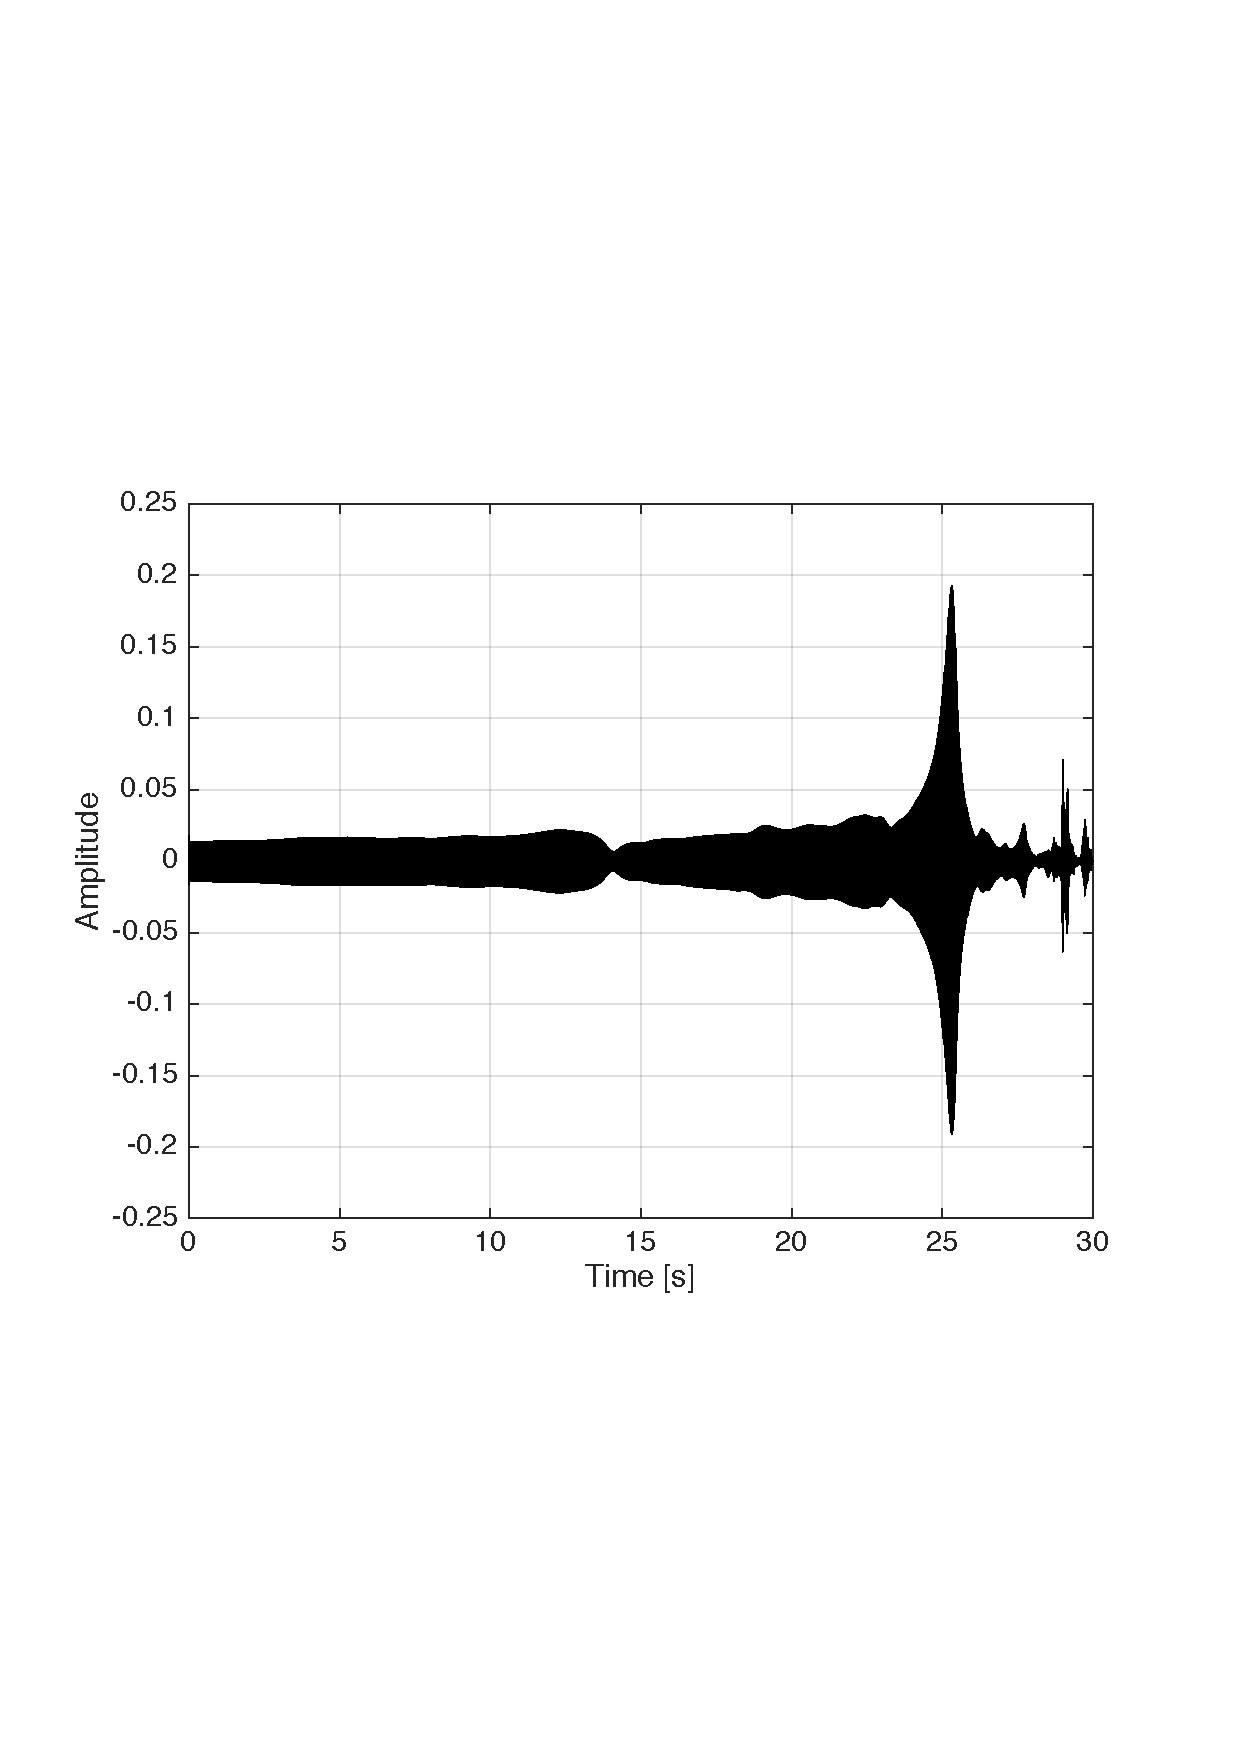
\includegraphics[width=\textwidth]{raw_driver19}
%% This file was created by matlab2tikz.
%
%The latest updates can be retrieved from
%  http://www.mathworks.com/matlabcentral/fileexchange/22022-matlab2tikz-matlab2tikz
%where you can also make suggestions and rate matlab2tikz.
%
\begin{tikzpicture}

\begin{axis}[%
width=1.6in,
height=1.2in,
at={(0.758in,0.481in)},
scale only axis,
xmin=0,
xmax=30,
xmajorgrids,
ymin=-0.2,
ymax=0.2,
ymajorgrids,
xlabel={Time [s]},
ylabel={Amplitude [V]},
axis background/.style={fill=white}
]
\addplot[fill=black,draw=black,forget plot] plot table[row sep=crcr]{%
2.08333333333333e-05	0.0174441337585449\\
0.0417454218822439	0.0131838321685791\\
0.0834700104311544	0.0131036043167114\\
0.125194598980065	0.0131006240844727\\
0.166919187528975	0.0131523609161377\\
0.208643776077886	0.0131937265396118\\
0.250368364626797	0.013242244720459\\
0.292092953175707	0.0132843255996704\\
0.333817541724618	0.0133000612258911\\
0.375542130273528	0.0133227109909058\\
0.417266718822439	0.0133814811706543\\
0.458991307371349	0.0134208202362061\\
0.50071589592026	0.0134570598602295\\
0.54244048446917	0.0134916305541992\\
0.584165073018081	0.0135313272476196\\
0.625889661566991	0.0135787725448608\\
0.667614250115902	0.0136535167694092\\
0.709338838664812	0.0136919021606445\\
0.751063427213723	0.0137407779693604\\
0.792788015762633	0.01378333568573\\
0.834512604311544	0.0138405561447144\\
0.876237192860454	0.0138554573059082\\
0.917961781409365	0.0138992071151733\\
0.959686369958275	0.0139317512512207\\
1.00141095850719	0.0139665603637695\\
1.0431355470561	0.0140010118484497\\
1.08486013560501	0.0140565633773804\\
1.12658472415392	0.0140770673751831\\
1.16830931270283	0.0141662359237671\\
1.21003390125174	0.0141417980194092\\
1.25175848980065	0.014143705368042\\
1.29348307834956	0.0142022371292114\\
1.33520766689847	0.014235258102417\\
1.37693225544738	0.0142310857772827\\
1.41865684399629	0.0142514705657959\\
1.4603814325452	0.0142501592636108\\
1.50210602109411	0.0142426490783691\\
1.54383060964302	0.0142196416854858\\
1.58555519819193	0.0141897201538086\\
1.62727978674084	0.0141717195510864\\
1.66900437528975	0.0141562223434448\\
1.71072896383866	0.0141338109970093\\
1.75245355238758	0.0141158103942871\\
1.79417814093649	0.0141069889068604\\
1.8359027294854	0.014079213142395\\
1.87762731803431	0.0140920877456665\\
1.91935190658322	0.0140824317932129\\
1.96107649513213	0.014080286026001\\
2.00280108368104	0.0140819549560547\\
2.04452567222995	0.0140804052352905\\
2.08625026077886	0.0140907764434814\\
2.12797484932777	0.0141453742980957\\
2.16969943787668	0.0141212940216064\\
2.21142402642559	0.014117956161499\\
2.2531486149745	0.0141592025756836\\
2.29487320352341	0.0141942501068115\\
2.33659779207232	0.0142147541046143\\
2.37832238062123	0.014255166053772\\
2.42004696917014	0.0142718553543091\\
2.46177155771905	0.0143097639083862\\
2.50349614626796	0.0143415927886963\\
2.54522073481687	0.0143803358078003\\
2.58694532336579	0.0144282579421997\\
2.6286699119147	0.014466404914856\\
2.67039450046361	0.0145164728164673\\
2.71211908901252	0.0145268440246582\\
2.75384367756143	0.0145998001098633\\
2.79556826611034	0.014657735824585\\
2.83729285465925	0.0147078037261963\\
2.87901744320816	0.014757513999939\\
2.92074203175707	0.0148080587387085\\
2.96246662030598	0.0148706436157227\\
3.00419120885489	0.0149272680282593\\
3.0459157974038	0.0149846076965332\\
3.08764038595271	0.0150657892227173\\
3.12936497450162	0.0151398181915283\\
3.17108956305053	0.0152368545532227\\
3.21281415159944	0.0153077840805054\\
3.25453874014835	0.0153566598892212\\
3.29626332869726	0.0154335498809814\\
3.33798791724618	0.0155411958694458\\
3.37971250579509	0.0155764818191528\\
3.421437094344	0.0156253576278687\\
3.46316168289291	0.0156955718994141\\
3.50488627144182	0.015771746635437\\
3.54661085999073	0.0158456563949585\\
3.58833544853964	0.0159142017364502\\
3.63006003708855	0.0159842967987061\\
3.67178462563746	0.0160502195358276\\
3.71350921418637	0.0160926580429077\\
3.75523380273528	0.0161477327346802\\
3.79695839128419	0.01618492603302\\
3.8386829798331	0.0162196159362793\\
3.88040756838201	0.0162382125854492\\
3.92213215693092	0.0162550210952759\\
3.96385674547983	0.0162825584411621\\
4.00558133402874	0.0162662267684937\\
4.04730592257765	0.0162646770477295\\
4.08903051112656	0.0162562131881714\\
4.13075509967547	0.0162286758422852\\
4.17247968822439	0.0162371397018433\\
4.2142042767733	0.0162320137023926\\
4.25592886532221	0.0162011384963989\\
4.29765345387112	0.0161941051483154\\
4.33937804242003	0.0161887407302856\\
4.38110263096894	0.0161789655685425\\
4.42282721951785	0.0162254571914673\\
4.46455180806676	0.0162070989608765\\
4.50627639661567	0.0162445306777954\\
4.54800098516458	0.0162758827209473\\
4.58972557371349	0.0163146257400513\\
4.6314501622624	0.0163501501083374\\
4.67317475081131	0.0163940191268921\\
4.71489933936022	0.0164343118667603\\
4.75662392790913	0.0164703130722046\\
4.79834851645804	0.0165045261383057\\
4.84007310500695	0.0165075063705444\\
4.88179769355586	0.0165128707885742\\
4.92352228210478	0.0165145397186279\\
4.96524687065368	0.0165392160415649\\
5.0069714592026	0.0165344476699829\\
5.04869604775151	0.0165383815765381\\
5.09042063630042	0.0165327787399292\\
5.13214522484933	0.0165436267852783\\
5.17386981339824	0.0165482759475708\\
5.21559440194715	0.0165524482727051\\
5.25731899049606	0.0165770053863525\\
5.29904357904497	0.0165486335754395\\
5.34076816759388	0.016539454460144\\
5.38249275614279	0.0165292024612427\\
5.4242173446917	0.0165091753005981\\
5.46594193324061	0.01650071144104\\
5.50766652178952	0.0164941549301147\\
5.54939111033843	0.0164557695388794\\
5.59111569888734	0.0164422988891602\\
5.63284028743625	0.0164107084274292\\
5.67456487598516	0.0163847208023071\\
5.71628946453407	0.0163488388061523\\
5.75801405308299	0.0162984132766724\\
5.7997386416319	0.016254186630249\\
5.84146323018081	0.0161999464035034\\
5.88318781872972	0.0161627531051636\\
5.92491240727863	0.016115665435791\\
5.96663699582754	0.0160861015319824\\
6.00836158437645	0.0160255432128906\\
6.05008617292536	0.0159963369369507\\
6.09181076147427	0.0159608125686646\\
6.13353535002318	0.015892505645752\\
6.17525993857209	0.0158644914627075\\
6.216984527121	0.0158439874649048\\
6.25870911566991	0.0158376693725586\\
6.30043370421882	0.015795111656189\\
6.34215829276773	0.0157642364501953\\
6.38388288131664	0.0157539844512939\\
6.42560746986555	0.0157680511474609\\
6.46733205841446	0.0157626867294312\\
6.50905664696338	0.0157822370529175\\
6.55078123551229	0.0157889127731323\\
6.5925058240612	0.01578688621521\\
6.63423041261011	0.015788197517395\\
6.67595500115902	0.0158027410507202\\
6.71767958970793	0.0158090591430664\\
6.75940417825684	0.0158181190490723\\
6.80112876680575	0.0158118009567261\\
6.84285335535466	0.0158218145370483\\
6.88457794390357	0.0158369541168213\\
6.92630253245248	0.0158761739730835\\
6.96802712100139	0.0158882141113281\\
7.0097517095503	0.0159152746200562\\
7.05147629809921	0.015964150428772\\
7.09320088664812	0.0159767866134644\\
7.13492547519703	0.0160250663757324\\
7.17665006374594	0.0161073207855225\\
7.21837465229485	0.0161528587341309\\
7.26009924084376	0.0162261724472046\\
7.30182382939268	0.0163071155548096\\
7.34354841794159	0.0163383483886719\\
7.3852730064905	0.016379714012146\\
7.42699759503941	0.0164109468460083\\
7.46872218358832	0.0164202451705933\\
7.51044677213723	0.01641845703125\\
7.55217136068614	0.0163893699645996\\
7.59389594923505	0.0163551568984985\\
7.63562053778396	0.016291618347168\\
7.67734512633287	0.0162198543548584\\
7.71906971488178	0.0161285400390625\\
7.76079430343069	0.016048789024353\\
7.8025188919796	0.0159471035003662\\
7.84424348052851	0.0158181190490723\\
7.88596806907742	0.0157514810562134\\
7.92769265762633	0.0156846046447754\\
7.96941724617524	0.0156430006027222\\
8.01114183472416	0.0156441926956177\\
8.05286642327307	0.015630841255188\\
8.09459101182198	0.0156680345535278\\
8.13631560037089	0.015711784362793\\
8.1780401889198	0.0157798528671265\\
8.21976477746871	0.0158299207687378\\
8.26148936601762	0.0159074068069458\\
8.30321395456653	0.0159891843795776\\
8.34493854311544	0.01605224609375\\
8.38666313166435	0.0161564350128174\\
8.42838772021326	0.0162137746810913\\
8.47011230876217	0.0163058042526245\\
8.51183689731108	0.0163658857345581\\
8.55356148585999	0.0164523124694824\\
8.5952860744089	0.0164806842803955\\
8.63701066295781	0.0166155099868774\\
8.67873525150672	0.0166575908660889\\
8.72045984005563	0.0167548656463623\\
8.76218442860454	0.016825795173645\\
8.80390901715345	0.0169020891189575\\
8.84563360570237	0.0169821977615356\\
8.88735819425128	0.0170701742172241\\
8.92908278280018	0.0171375274658203\\
8.9708073713491	0.0171587467193604\\
9.01253195989801	0.017237663269043\\
9.05425654844692	0.0172935724258423\\
9.09598113699583	0.0173218250274658\\
9.13770572554474	0.0173497200012207\\
9.17943031409365	0.0173822641372681\\
9.22115490264256	0.0174020528793335\\
9.26287949119147	0.0174028873443604\\
9.30460407974038	0.0174020528793335\\
9.34632866828929	0.017397403717041\\
9.3880532568382	0.017382025718689\\
9.42977784538711	0.0173323154449463\\
9.47150243393602	0.0173298120498657\\
9.51322702248493	0.0173071622848511\\
9.55495161103384	0.0172981023788452\\
9.59667619958275	0.0172533988952637\\
9.63840078813166	0.0172268152236938\\
9.68012537668058	0.0172126293182373\\
9.72184996522949	0.0172011852264404\\
9.7635745537784	0.0171804428100586\\
9.80529914232731	0.0171520709991455\\
9.84702373087622	0.0171386003494263\\
9.88874831942513	0.0171166658401489\\
9.93047290797404	0.0170993804931641\\
9.97219749652295	0.0170501470565796\\
10.0139220850719	0.0170356035232544\\
10.0556466736208	0.0170102119445801\\
10.0973712621697	0.0169705152511597\\
10.1390958507186	0.0169491767883301\\
10.1808204392675	0.0169264078140259\\
10.2225450278164	0.0169349908828735\\
10.2642696163653	0.016948938369751\\
10.3059942049142	0.0169826745986938\\
10.3477187934631	0.0170327425003052\\
10.3894433820121	0.0170915126800537\\
10.431167970561	0.0171574354171753\\
10.4728925591099	0.0172317028045654\\
10.5146171476588	0.0172722339630127\\
10.5563417362077	0.0173627138137817\\
10.5980663247566	0.0174278020858765\\
10.6397909133055	0.0175130367279053\\
10.6815155018544	0.0175483226776123\\
10.7232400904033	0.0176342725753784\\
10.7649646789523	0.0176903009414673\\
10.8066892675012	0.0177403688430786\\
10.8484138560501	0.0177834033966064\\
10.890138444599	0.0178585052490234\\
10.9318630331479	0.0179126262664795\\
10.9735876216968	0.0179930925369263\\
11.0153122102457	0.0180377960205078\\
11.0570367987946	0.0181233882904053\\
11.0987613873435	0.0181983709335327\\
11.1404859758924	0.0183128118515015\\
11.1822105644414	0.0184154510498047\\
11.2239351529903	0.0185511112213135\\
11.2656597415392	0.0186648368835449\\
11.3073843300881	0.0188018083572388\\
11.349108918637	0.0189625024795532\\
11.3908335071859	0.0190943479537964\\
11.4325580957348	0.0192328691482544\\
11.4742826842837	0.0194246768951416\\
11.5160072728326	0.0195508003234863\\
11.5577318613816	0.019692063331604\\
11.5994564499305	0.0198198556900024\\
11.6411810384794	0.0199755430221558\\
11.6829056270283	0.0201060771942139\\
11.7246302155772	0.0202442407608032\\
11.7663548041261	0.0203926563262939\\
11.808079392675	0.0205307006835938\\
11.8498039812239	0.0206559896469116\\
11.8915285697728	0.0208258628845215\\
11.9332531583217	0.0209463834762573\\
11.9749777468707	0.0210902690887451\\
12.0167023354196	0.0212063789367676\\
12.0584269239685	0.0213172435760498\\
12.1001515125174	0.0214052200317383\\
12.1418761010663	0.0215300321578979\\
12.1836006896152	0.0216346979141235\\
12.2253252781641	0.0217214822769165\\
12.267049866713	0.0217512845993042\\
12.3087744552619	0.0217386484146118\\
12.3504990438108	0.0217629671096802\\
12.3922236323598	0.0217190980911255\\
12.4339482209087	0.0217164754867554\\
12.4756728094576	0.0216211080551147\\
12.5173973980065	0.0215216875076294\\
12.5591219865554	0.0214111804962158\\
12.6008465751043	0.0212830305099487\\
12.6425711636532	0.0211762189865112\\
12.6842957522021	0.0210355520248413\\
12.726020340751	0.0209170579910278\\
12.7677449293	0.0208185911178589\\
12.8094695178489	0.0207177400588989\\
12.8511941063978	0.0206308364868164\\
12.8929186949467	0.0205261707305908\\
12.9346432834956	0.0204188823699951\\
12.9763678720445	0.0203160047531128\\
13.0180924605934	0.0202019214630127\\
13.0598170491423	0.020089864730835\\
13.1015416376912	0.0199722051620483\\
13.1432662262401	0.0198445320129395\\
13.1849908147891	0.0197038650512695\\
13.226715403338	0.0195189714431763\\
13.2684399918869	0.0193073749542236\\
13.3101645804358	0.0190596580505371\\
13.3518891689847	0.0188181400299072\\
13.3936137575336	0.0185122489929199\\
13.4353383460825	0.0181918144226074\\
13.4770629346314	0.0177853107452393\\
13.5187875231803	0.0173110961914063\\
13.5605121117293	0.0167787075042725\\
13.6022367002782	0.0161740779876709\\
13.6439612888271	0.0155293941497803\\
13.685685877376	0.0147796869277954\\
13.7274104659249	0.0139639377593994\\
13.7691350544738	0.0130655765533447\\
13.8108596430227	0.0121190547943115\\
13.8525842315716	0.011111855506897\\
13.8943088201205	0.0100915431976318\\
13.9360334086694	0.00906765460968018\\
13.9777579972184	0.0081101655960083\\
14.0194825857673	0.00735759735107422\\
14.0612071743162	0.00674760341644287\\
14.1029317628651	0.00652647018432617\\
14.144656351414	0.00688815116882324\\
14.1863809399629	0.00745463371276855\\
14.2281055285118	0.00815272331237793\\
14.2698301170607	0.00885546207427979\\
14.3115547056096	0.00954830646514893\\
14.3532792941586	0.0101321935653687\\
14.3950038827075	0.0106920003890991\\
14.4367284712564	0.0111517906188965\\
14.4784530598053	0.0115351676940918\\
14.5201776483542	0.0118722915649414\\
14.5619022369031	0.0121043920516968\\
14.603626825452	0.0123043060302734\\
14.6453514140009	0.0124328136444092\\
14.6870760025498	0.0125536918640137\\
14.7288005910988	0.0126279592514038\\
14.7705251796477	0.0126522779464722\\
14.8122497681966	0.0126771926879883\\
14.8539743567455	0.0126643180847168\\
14.8956989452944	0.0126442909240723\\
14.9374235338433	0.0126314163208008\\
14.9791481223922	0.0126005411148071\\
15.0208727109411	0.0125870704650879\\
15.06259729949	0.0126197338104248\\
15.1043218880389	0.0127360820770264\\
15.1460464765879	0.0129470825195313\\
15.1877710651368	0.0131411552429199\\
15.2294956536857	0.0134528875350952\\
15.2712202422346	0.0137631893157959\\
15.3129448307835	0.014081597328186\\
15.3546694193324	0.0143324136734009\\
15.3963940078813	0.0145440101623535\\
15.4381185964302	0.0147069692611694\\
15.4798431849791	0.014826774597168\\
15.521567773528	0.0149147510528564\\
15.563292362077	0.0150187015533447\\
15.6050169506259	0.0150867700576782\\
15.6467415391748	0.0151418447494507\\
15.6884661277237	0.0152006149291992\\
15.7301907162726	0.0152875185012817\\
15.7719153048215	0.015317440032959\\
15.8136398933704	0.0153570175170898\\
15.8553644819193	0.0153845548629761\\
15.8970890704682	0.0154201984405518\\
15.9388136590172	0.0154287815093994\\
15.9805382475661	0.0154200792312622\\
16.022262836115	0.0154227018356323\\
16.0639874246639	0.0153900384902954\\
16.1057120132128	0.0153504610061646\\
16.1474366017617	0.0152820348739624\\
16.1891611903106	0.0152740478515625\\
16.2308857788595	0.0152736902236938\\
16.2726103674084	0.0152853727340698\\
16.3143349559573	0.0153579711914063\\
16.3560595445063	0.0154263973236084\\
16.3977841330552	0.0155422687530518\\
16.4395087216041	0.0156645774841309\\
16.481233310153	0.015790581703186\\
16.5229578987019	0.0159449577331543\\
16.5646824872508	0.0161056518554688\\
16.6064070757997	0.0162507295608521\\
16.6481316643486	0.0163685083389282\\
16.6898562528975	0.0164653062820435\\
16.7315808414465	0.0165603160858154\\
16.7733054299954	0.0167076587677002\\
16.8150300185443	0.0167895555496216\\
16.8567546070932	0.0168788433074951\\
16.8984791956421	0.0169848203659058\\
16.940203784191	0.017051100730896\\
16.9819283727399	0.017139196395874\\
17.0236529612888	0.0172312259674072\\
17.0653775498377	0.0173563957214355\\
17.1071021383867	0.0174448490142822\\
17.1488267269356	0.0174803733825684\\
17.1905513154845	0.0175639390945435\\
17.2322759040334	0.0176322460174561\\
17.2740004925823	0.0177028179168701\\
17.3157250811312	0.017791748046875\\
17.3574496696801	0.0178496837615967\\
17.399174258229	0.0178979635238647\\
17.4408988467779	0.017961859703064\\
17.4826234353268	0.018022894859314\\
17.5243480238758	0.018062949180603\\
17.5660726124247	0.01810622215271\\
17.6077972009736	0.0180763006210327\\
17.6495217895225	0.0180815458297729\\
17.6912463780714	0.0180732011795044\\
17.7329709666203	0.0180991888046265\\
17.7746955551692	0.0181357860565186\\
17.8164201437181	0.018202543258667\\
17.858144732267	0.0183231830596924\\
17.8998693208159	0.0184512138366699\\
17.9415939093649	0.0185703039169312\\
17.9833184979138	0.0187492370605469\\
18.0250430864627	0.0189353227615356\\
18.0667676750116	0.0190675258636475\\
18.1084922635605	0.0192264318466187\\
18.1502168521094	0.0192973613739014\\
18.1919414406583	0.0193362236022949\\
18.2336660292072	0.0193533897399902\\
18.2753906177561	0.0193248987197876\\
18.3171152063051	0.0193346738815308\\
18.358839794854	0.0192720890045166\\
18.4005643834029	0.0192611217498779\\
18.4422889719518	0.0192636251449585\\
18.4840135605007	0.0192739963531494\\
18.5257381490496	0.0192903280258179\\
18.5674627375985	0.0194275379180908\\
18.6091873261474	0.0196996927261353\\
18.6509119146963	0.0200306177139282\\
18.6926365032453	0.0204979181289673\\
18.7343610917942	0.02104651927948\\
18.7760856803431	0.0216186046600342\\
18.817810268892	0.0222443342208862\\
18.8595348574409	0.0227910280227661\\
18.9012594459898	0.0233092308044434\\
18.9429840345387	0.023730993270874\\
18.9847086230876	0.0240856409072876\\
19.0264332116365	0.0244448184967041\\
19.0681578001854	0.0246785879135132\\
19.1098823887344	0.0248157978057861\\
19.1516069772833	0.0248291492462158\\
19.1933315658322	0.0247887372970581\\
19.2350561543811	0.0246955156326294\\
19.27678074293	0.0245308876037598\\
19.3185053314789	0.0243546962738037\\
19.3602299200278	0.0240871906280518\\
19.4019545085767	0.0237839221954346\\
19.4436790971256	0.0234526395797729\\
19.4854036856745	0.0231184959411621\\
19.5271282742235	0.022815465927124\\
19.5688528627724	0.0225284099578857\\
19.6105774513213	0.0223060846328735\\
19.6523020398702	0.0221070051193237\\
19.6940266284191	0.0219635963439941\\
19.735751216968	0.0218530893325806\\
19.7774758055169	0.0217581987380981\\
19.8192003940658	0.0217596292495728\\
19.8609249826147	0.0217828750610352\\
19.9026495711637	0.0218667984008789\\
19.9443741597126	0.0219509601593018\\
19.9860987482615	0.0220874547958374\\
20.0278233368104	0.0222543478012085\\
20.0695479253593	0.0224721431732178\\
20.1112725139082	0.0226690769195557\\
20.1529971024571	0.0229157209396362\\
20.194721691006	0.0231697559356689\\
20.2364462795549	0.0234352350234985\\
20.2781708681038	0.0237188339233398\\
20.3198954566528	0.0240160226821899\\
20.3616200452017	0.0242964029312134\\
20.4033446337506	0.024566650390625\\
20.4450692222995	0.0247782468795776\\
20.4867938108484	0.0249801874160767\\
20.5285183993973	0.025060772895813\\
20.5702429879462	0.0250948667526245\\
20.6119675764951	0.0251015424728394\\
20.653692165044	0.025084376335144\\
20.695416753593	0.0250260829925537\\
20.7371413421419	0.0249568223953247\\
20.7788659306908	0.0249083042144775\\
20.8205905192397	0.0248545408248901\\
20.8623151077886	0.0248538255691528\\
20.9040396963375	0.0248321294784546\\
20.9457642848864	0.0248123407363892\\
20.9874888734353	0.0247715711593628\\
21.0292134619842	0.0246872901916504\\
21.0709380505331	0.0245916843414307\\
21.1126626390821	0.0244895219802856\\
21.154387227631	0.0243560075759888\\
21.1961118161799	0.0242257118225098\\
21.2378364047288	0.0241231918334961\\
21.2795609932777	0.0240743160247803\\
21.3212855818266	0.0240955352783203\\
21.3630101703755	0.0242211818695068\\
21.4047347589244	0.0243576765060425\\
21.4464593474733	0.0245411396026611\\
21.4881839360223	0.0248323678970337\\
21.5299085245712	0.0251299142837524\\
21.5716331131201	0.0254895687103271\\
21.613357701669	0.0259164571762085\\
21.6550822902179	0.0263410806655884\\
21.6968068787668	0.0268235206604004\\
21.7385314673157	0.0273033380508423\\
21.7802560558646	0.0278036594390869\\
21.8219806444135	0.0282833576202393\\
21.8637052329624	0.0288461446762085\\
21.9054298215114	0.0293409824371338\\
21.9471544100603	0.0298067331314087\\
21.9888789986092	0.0302213430404663\\
22.0306035871581	0.0305540561676025\\
22.072328175707	0.0307530164718628\\
22.1140527642559	0.0307987928390503\\
22.1557773528048	0.030825138092041\\
22.1975019413537	0.0308418273925781\\
22.2392265299026	0.0311071872711182\\
22.2809511184516	0.0313805341720581\\
22.3226757070005	0.0317173004150391\\
22.3644002955494	0.0320000648498535\\
22.4061248840983	0.0321570634841919\\
22.4478494726472	0.0321915149688721\\
22.4895740611961	0.0321606397628784\\
22.531298649745	0.031922459602356\\
22.5730232382939	0.0316141843795776\\
22.6147478268428	0.0312548875808716\\
22.6564724153917	0.0308171510696411\\
22.6981970039407	0.0305826663970947\\
22.7399215924896	0.0304679870605469\\
22.7816461810385	0.0303603410720825\\
22.8233707695874	0.0304563045501709\\
22.8650953581363	0.0305367708206177\\
22.9068199466852	0.0306057929992676\\
22.9485445352341	0.0306912660598755\\
22.990269123783	0.0306066274642944\\
23.0319937123319	0.0304591655731201\\
23.0737183008809	0.0297863483428955\\
23.1154428894298	0.0285071134567261\\
23.1571674779787	0.027154803276062\\
23.1988920665276	0.0259910821914673\\
23.2406166550765	0.0244603157043457\\
23.2823412436254	0.0236220359802246\\
23.3240658321743	0.0235285758972168\\
23.3657904207232	0.0241098403930664\\
23.4075150092721	0.0248513221740723\\
23.449239597821	0.0258579254150391\\
23.49096418637	0.0267441272735596\\
23.5326887749189	0.0276174545288086\\
23.5744133634678	0.0282967090606689\\
23.6161379520167	0.0288980007171631\\
23.6578625405656	0.0294115543365479\\
23.6995871291145	0.0299835205078125\\
23.7413117176634	0.0305644273757935\\
23.7830363062123	0.0313618183135986\\
23.8247608947612	0.0322580337524414\\
23.8664854833102	0.0332018136978149\\
23.9082100718591	0.0342499017715454\\
23.949934660408	0.035599946975708\\
23.9916592489569	0.0370364189147949\\
24.0333838375058	0.0383732318878174\\
24.0751084260547	0.0398944616317749\\
24.1168330146036	0.041479229927063\\
24.1585576031525	0.0429228544235229\\
24.2002821917014	0.0444319248199463\\
24.2420067802503	0.0459293127059937\\
24.2837313687993	0.047610878944397\\
24.3254559573482	0.0492688417434692\\
24.3671805458971	0.0510417222976685\\
24.408905134446	0.0529109239578247\\
24.4506297229949	0.0548422336578369\\
24.4923543115438	0.056898832321167\\
24.5340789000927	0.0591094493865967\\
24.5758034886416	0.0617804527282715\\
24.6175280771905	0.0645843744277954\\
24.6592526657395	0.0677156448364258\\
24.7009772542884	0.0712670087814331\\
24.7427018428373	0.0752949714660645\\
24.7844264313862	0.0799596309661865\\
24.8261510199351	0.0852384567260742\\
24.867875608484	0.0909876823425293\\
24.9096001970329	0.0979855060577393\\
24.9513247855818	0.105462312698364\\
24.9930493741307	0.114107251167297\\
25.0347739626796	0.123892664909363\\
25.0764985512286	0.1347895860672\\
25.1182231397775	0.146229147911072\\
25.1599477283264	0.158706545829773\\
25.2016723168753	0.170397281646729\\
25.2433969054242	0.181927919387817\\
25.2851214939731	0.190452098846436\\
25.326846082522	0.192880272865295\\
25.3685706710709	0.192157387733459\\
25.4102952596198	0.181955933570862\\
25.4520198481687	0.162297606468201\\
25.4937444367177	0.13434636592865\\
25.5354690252666	0.109553933143616\\
25.5771936138155	0.0896941423416138\\
25.6189182023644	0.0760148763656616\\
25.6606427909133	0.0651895999908447\\
25.7023673794622	0.0563890933990479\\
25.7440919680111	0.0492444038391113\\
25.78581655656	0.043710470199585\\
25.8275411451089	0.0384472608566284\\
25.8692657336579	0.0339940786361694\\
25.9109903222068	0.0300600528717041\\
25.9527149107557	0.0264880657196045\\
25.9944394993046	0.0233311653137207\\
26.0361640878535	0.0206685066223145\\
26.0778886764024	0.0186737775802612\\
26.1196132649513	0.0171686410903931\\
26.1613378535002	0.0166844129562378\\
26.2030624420491	0.017844557762146\\
26.2447870305981	0.0197421312332153\\
26.286511619147	0.0215028524398804\\
26.3282362076959	0.0223579406738281\\
26.3699607962448	0.0223031044006348\\
26.4116853847937	0.0217078924179077\\
26.4534099733426	0.0204193592071533\\
26.4951345618915	0.0195810794830322\\
26.5368591504404	0.0191034078598022\\
26.5785837389893	0.0182909965515137\\
26.6203083275383	0.01659095287323\\
26.6620329160872	0.0147438049316406\\
26.7037575046361	0.0134490728378296\\
26.745482093185	0.012037992477417\\
26.7872066817339	0.0107738971710205\\
26.8289312702828	0.00990462303161621\\
26.8706558588317	0.00957143306732178\\
26.9123804473806	0.00931215286254883\\
26.9541050359295	0.0092695951461792\\
26.9958296244784	0.0102084875106812\\
27.0375542130274	0.0113158226013184\\
27.0792788015763	0.0121122598648071\\
27.1210033901252	0.0121549367904663\\
27.1627279786741	0.0111083984375\\
27.204452567223	0.00957083702087402\\
27.2461771557719	0.00859379768371582\\
27.2879017443208	0.00834882259368896\\
27.3296263328697	0.00859546661376953\\
27.3713509214186	0.0090184211730957\\
27.4130755099675	0.00977170467376709\\
27.4548000985165	0.0107346773147583\\
27.4965246870654	0.012182354927063\\
27.5382492756143	0.0141066312789917\\
27.5799738641632	0.0166143178939819\\
27.6216984527121	0.0203871726989746\\
27.663423041261	0.0240563154220581\\
27.7051476298099	0.0260938405990601\\
27.7468722183588	0.0261249542236328\\
27.7885968069077	0.0226942300796509\\
27.8303213954567	0.0153995752334595\\
27.8720459840056	0.0115272998809814\\
27.9137705725545	0.00934135913848877\\
27.9554951611034	0.00725364685058594\\
27.9972197496523	0.00573289394378662\\
28.0389443382012	0.00476109981536865\\
28.0806689267501	0.00405430793762207\\
28.122393515299	0.00347089767456055\\
28.1641181038479	0.00348937511444092\\
28.2058426923968	0.0043492317199707\\
28.2475672809458	0.00484251976013184\\
28.2892918694947	0.00487172603607178\\
28.3310164580436	0.00547254085540771\\
28.3727410465925	0.00589895248413086\\
28.4144656351414	0.00629270076751709\\
28.4561902236903	0.00670242309570313\\
28.4979148122392	0.00694727897644043\\
28.5396394007881	0.00746893882751465\\
28.581363989337	0.00698328018188477\\
28.623088577886	0.00598013401031494\\
28.6648131664349	0.0123151540756226\\
28.7065377549838	0.0124528408050537\\
28.7482623435327	0.0158895254135132\\
28.7899869320816	0.0123809576034546\\
28.8317115206305	0.00990724563598633\\
28.8734361091794	0.0101600885391235\\
28.9151606977283	0.00902903079986572\\
28.9568852862772	0.00959169864654541\\
28.9986098748261	0.0708549022674561\\
29.0403344633751	0.0490773916244507\\
29.082059051924	0.0367391109466553\\
29.1237836404729	0.0392665863037109\\
29.1655082290218	0.0501984357833862\\
29.2072328175707	0.0316517353057861\\
29.2489574061196	0.0146907567977905\\
29.2906819946685	0.0124069452285767\\
29.3324065832174	0.0109615325927734\\
29.3741311717663	0.00983536243438721\\
29.4158557603153	0.00371837615966797\\
29.4575803488642	0.00346684455871582\\
29.4993049374131	0.0025477409362793\\
29.541029525962	0.0020139217376709\\
29.5827541145109	0.00222396850585938\\
29.6244787030598	0.0047835111618042\\
29.6662032916087	0.0106549263000488\\
29.7079278801576	0.0227276086807251\\
29.7496524687065	0.0288950204849243\\
29.7913770572554	0.0240693092346191\\
29.8331016458044	0.0165066719055176\\
29.8748262343533	0.0114091634750366\\
29.9165508229022	0.00875699520111084\\
29.9582754114511	0.00749635696411133\\
30	0.00196146965026855\\
}
\closedcycle;
\addplot[fill=black,draw=black,forget plot] plot table[row sep=crcr]{%
2.08333333333333e-05	-0.0159932374954224\\
0.0417454218822439	-0.0136831998825073\\
0.0834700104311544	-0.0136864185333252\\
0.125194598980065	-0.0137081146240234\\
0.166919187528975	-0.0137027502059937\\
0.208643776077886	-0.0137177705764771\\
0.250368364626797	-0.0137653350830078\\
0.292092953175707	-0.0137816667556763\\
0.333817541724618	-0.0138300657272339\\
0.375542130273528	-0.0138695240020752\\
0.417266718822439	-0.0139075517654419\\
0.458991307371349	-0.0139497518539429\\
0.50071589592026	-0.0140053033828735\\
0.54244048446917	-0.0140515565872192\\
0.584165073018081	-0.0140962600708008\\
0.625889661566991	-0.0141353607177734\\
0.667614250115902	-0.0141550302505493\\
0.709338838664812	-0.0141642093658447\\
0.751063427213723	-0.0142364501953125\\
0.792788015762633	-0.0142496824264526\\
0.834512604311544	-0.0143007040023804\\
0.876237192860454	-0.0143524408340454\\
0.917961781409365	-0.0143682956695557\\
0.959686369958275	-0.0144027471542358\\
1.00141095850719	-0.0144290924072266\\
1.0431355470561	-0.0144684314727783\\
1.08486013560501	-0.0145009756088257\\
1.12658472415392	-0.0145292282104492\\
1.16830931270283	-0.0145310163497925\\
1.21003390125174	-0.0145913362503052\\
1.25175848980065	-0.0146056413650513\\
1.29348307834956	-0.014609694480896\\
1.33520766689847	-0.014613151550293\\
1.37693225544738	-0.0146564245223999\\
1.41865684399629	-0.0147069692611694\\
1.4603814325452	-0.0147548913955688\\
1.50210602109411	-0.0147720575332642\\
1.54383060964302	-0.0147882699966431\\
1.58555519819193	-0.0148137807846069\\
1.62727978674084	-0.0147954225540161\\
1.66900437528975	-0.0147997140884399\\
1.71072896383866	-0.014802098274231\\
1.75245355238758	-0.0147850513458252\\
1.79417814093649	-0.0147900581359863\\
1.8359027294854	-0.0147967338562012\\
1.87762731803431	-0.0147658586502075\\
1.91935190658322	-0.0147805213928223\\
1.96107649513213	-0.0147795677185059\\
2.00280108368104	-0.0147765874862671\\
2.04452567222995	-0.0148054361343384\\
2.08625026077886	-0.0148167610168457\\
2.12797484932777	-0.0148104429244995\\
2.16969943787668	-0.014845609664917\\
2.21142402642559	-0.0148526430130005\\
2.2531486149745	-0.0148493051528931\\
2.29487320352341	-0.0148800611495972\\
2.33659779207232	-0.0149073600769043\\
2.37832238062123	-0.0149215459823608\\
2.42004696917014	-0.0149686336517334\\
2.46177155771905	-0.0149891376495361\\
2.50349614626796	-0.0150300264358521\\
2.54522073481687	-0.015070915222168\\
2.58694532336579	-0.0150928497314453\\
2.6286699119147	-0.0151451826095581\\
2.67039450046361	-0.0151525735855103\\
2.71211908901252	-0.0152038335800171\\
2.75384367756143	-0.0152643918991089\\
2.79556826611034	-0.0153129100799561\\
2.83729285465925	-0.0153428316116333\\
2.87901744320816	-0.0154058933258057\\
2.92074203175707	-0.015446662902832\\
2.96246662030598	-0.0155152082443237\\
3.00419120885489	-0.0156008005142212\\
3.0459157974038	-0.015687108039856\\
3.08764038595271	-0.015765905380249\\
3.12936497450162	-0.0158531665802002\\
3.17108956305053	-0.0159111022949219\\
3.21281415159944	-0.0159949064254761\\
3.25453874014835	-0.0161058902740479\\
3.29626332869726	-0.0161623954772949\\
3.33798791724618	-0.0162557363510132\\
3.37971250579509	-0.0163384675979614\\
3.421437094344	-0.0164409875869751\\
3.46316168289291	-0.0165195465087891\\
3.50488627144182	-0.0165740251541138\\
3.54661085999073	-0.0166549682617188\\
3.58833544853964	-0.0167381763458252\\
3.63006003708855	-0.0167884826660156\\
3.67178462563746	-0.0168477296829224\\
3.71350921418637	-0.016872763633728\\
3.75523380273528	-0.0168941020965576\\
3.79695839128419	-0.0169187784194946\\
3.8386829798331	-0.0169479846954346\\
3.88040756838201	-0.0169333219528198\\
3.92213215693092	-0.016893744468689\\
3.96385674547983	-0.0169346332550049\\
4.00558133402874	-0.0168807506561279\\
4.04730592257765	-0.0168675184249878\\
4.08903051112656	-0.0168465375900269\\
4.13075509967547	-0.0168452262878418\\
4.17247968822439	-0.0168131589889526\\
4.2142042767733	-0.0167852640151978\\
4.25592886532221	-0.0167598724365234\\
4.29765345387112	-0.0167505741119385\\
4.33937804242003	-0.016740083694458\\
4.38110263096894	-0.0167372226715088\\
4.42282721951785	-0.0167292356491089\\
4.46455180806676	-0.0167250633239746\\
4.50627639661567	-0.0167497396469116\\
4.54800098516458	-0.0167809724807739\\
4.58972557371349	-0.0168344974517822\\
4.6314501622624	-0.0168977975845337\\
4.67317475081131	-0.0169267654418945\\
4.71489933936022	-0.0169526338577271\\
4.75662392790913	-0.0169451236724854\\
4.79834851645804	-0.0169491767883301\\
4.84007310500695	-0.0169534683227539\\
4.88179769355586	-0.0169605016708374\\
4.92352228210478	-0.0169579982757568\\
4.96524687065368	-0.0169459581375122\\
5.0069714592026	-0.0169612169265747\\
5.04869604775151	-0.0169461965560913\\
5.09042063630042	-0.016968846321106\\
5.13214522484933	-0.0169471502304077\\
5.17386981339824	-0.0169591903686523\\
5.21559440194715	-0.016942024230957\\
5.25731899049606	-0.0169354677200317\\
5.29904357904497	-0.0169334411621094\\
5.34076816759388	-0.016936182975769\\
5.38249275614279	-0.0169117450714111\\
5.4242173446917	-0.0169116258621216\\
5.46594193324061	-0.0169053077697754\\
5.50766652178952	-0.01686692237854\\
5.54939111033843	-0.0168808698654175\\
5.59111569888734	-0.0168665647506714\\
5.63284028743625	-0.0168148279190063\\
5.67456487598516	-0.0167924165725708\\
5.71628946453407	-0.0167427062988281\\
5.75801405308299	-0.0167151689529419\\
5.7997386416319	-0.0166959762573242\\
5.84146323018081	-0.0166800022125244\\
5.88318781872972	-0.0166391134262085\\
5.92491240727863	-0.0166083574295044\\
5.96663699582754	-0.0165565013885498\\
6.00836158437645	-0.016548752784729\\
6.05008617292536	-0.0165069103240967\\
6.09181076147427	-0.0164694786071777\\
6.13353535002318	-0.016451358795166\\
6.17525993857209	-0.0164226293563843\\
6.216984527121	-0.0163737535476685\\
6.25870911566991	-0.0163513422012329\\
6.30043370421882	-0.0163525342941284\\
6.34215829276773	-0.0163525342941284\\
6.38388288131664	-0.0163518190383911\\
6.42560746986555	-0.0163501501083374\\
6.46733205841446	-0.0163429975509644\\
6.50905664696338	-0.0163670778274536\\
6.55078123551229	-0.0163668394088745\\
6.5925058240612	-0.0163979530334473\\
6.63423041261011	-0.0164004564285278\\
6.67595500115902	-0.0164167881011963\\
6.71767958970793	-0.01643967628479\\
6.75940417825684	-0.0164421796798706\\
6.80112876680575	-0.0164488554000854\\
6.84285335535466	-0.016448974609375\\
6.88457794390357	-0.016472339630127\\
6.92630253245248	-0.0165094137191772\\
6.96802712100139	-0.0165352821350098\\
7.0097517095503	-0.0165783166885376\\
7.05147629809921	-0.0166103839874268\\
7.09320088664812	-0.0166771411895752\\
7.13492547519703	-0.0167235136032104\\
7.17665006374594	-0.016762375831604\\
7.21837465229485	-0.0168224573135376\\
7.26009924084376	-0.0168670415878296\\
7.30182382939268	-0.0168749094009399\\
7.34354841794159	-0.0169117450714111\\
7.3852730064905	-0.0169516801834106\\
7.42699759503941	-0.0169820785522461\\
7.46872218358832	-0.0169767141342163\\
7.51044677213723	-0.0169795751571655\\
7.55217136068614	-0.0169461965560913\\
7.59389594923505	-0.0169112682342529\\
7.63562053778396	-0.016893744468689\\
7.67734512633287	-0.0167742967605591\\
7.71906971488178	-0.016714334487915\\
7.76079430343069	-0.0166012048721313\\
7.8025188919796	-0.0164294242858887\\
7.84424348052851	-0.0163884162902832\\
7.88596806907742	-0.0163111686706543\\
7.92769265762633	-0.0162628889083862\\
7.96941724617524	-0.0162183046340942\\
8.01114183472416	-0.0162019729614258\\
8.05286642327307	-0.0162206888198853\\
8.09459101182198	-0.0162594318389893\\
8.13631560037089	-0.0162904262542725\\
8.1780401889198	-0.0163576602935791\\
8.21976477746871	-0.0164244174957275\\
8.26148936601762	-0.0165115594863892\\
8.30321395456653	-0.0165975093841553\\
8.34493854311544	-0.0166696310043335\\
8.38666313166435	-0.0167193412780762\\
8.42838772021326	-0.0168086290359497\\
8.47011230876217	-0.0168790817260742\\
8.51183689731108	-0.0169645547866821\\
8.55356148585999	-0.0170485973358154\\
8.5952860744089	-0.017114520072937\\
8.63701066295781	-0.0171991586685181\\
8.67873525150672	-0.0172797441482544\\
8.72045984005563	-0.0173673629760742\\
8.76218442860454	-0.0174151659011841\\
8.80390901715345	-0.0174990892410278\\
8.84563360570237	-0.0175384283065796\\
8.88735819425128	-0.0175958871841431\\
8.92908278280018	-0.0176502466201782\\
8.9708073713491	-0.0177098512649536\\
9.01253195989801	-0.0177485942840576\\
9.05425654844692	-0.0177981853485107\\
9.09598113699583	-0.017824649810791\\
9.13770572554474	-0.0178617238998413\\
9.17943031409365	-0.017900824546814\\
9.22115490264256	-0.017920970916748\\
9.26287949119147	-0.017920970916748\\
9.30460407974038	-0.0179229974746704\\
9.34632866828929	-0.0179156064987183\\
9.3880532568382	-0.0178991556167603\\
9.42977784538711	-0.0179009437561035\\
9.47150243393602	-0.0178804397583008\\
9.51322702248493	-0.0178624391555786\\
9.55495161103384	-0.017827033996582\\
9.59667619958275	-0.0178166627883911\\
9.63840078813166	-0.0177962779998779\\
9.68012537668058	-0.0177731513977051\\
9.72184996522949	-0.0177674293518066\\
9.7635745537784	-0.0177444219589233\\
9.80529914232731	-0.0177211761474609\\
9.84702373087622	-0.0176931619644165\\
9.88874831942513	-0.0176559686660767\\
9.93047290797404	-0.0176379680633545\\
9.97219749652295	-0.017622709274292\\
10.0139220850719	-0.0175876617431641\\
10.0556466736208	-0.0175426006317139\\
10.0973712621697	-0.0175328254699707\\
10.1390958507186	-0.017499566078186\\
10.1808204392675	-0.0175129175186157\\
10.2225450278164	-0.0174999237060547\\
10.2642696163653	-0.0175207853317261\\
10.3059942049142	-0.0175470113754272\\
10.3477187934631	-0.0176101922988892\\
10.3894433820121	-0.0176711082458496\\
10.431167970561	-0.0177111625671387\\
10.4728925591099	-0.0177946090698242\\
10.5146171476588	-0.0178449153900146\\
10.5563417362077	-0.0179034471511841\\
10.5980663247566	-0.0179823637008667\\
10.6397909133055	-0.0180490016937256\\
10.6815155018544	-0.018073558807373\\
10.7232400904033	-0.0181691646575928\\
10.7649646789523	-0.0182160139083862\\
10.8066892675012	-0.018257737159729\\
10.8484138560501	-0.018315315246582\\
10.890138444599	-0.0183507204055786\\
10.9318630331479	-0.0184015035629272\\
10.9735876216968	-0.0184750556945801\\
11.0153122102457	-0.0185734033584595\\
11.0570367987946	-0.018660306930542\\
11.0987613873435	-0.0187779664993286\\
11.1404859758924	-0.0188738107681274\\
11.1822105644414	-0.0190337896347046\\
11.2239351529903	-0.0191354751586914\\
11.2656597415392	-0.019279956817627\\
11.3073843300881	-0.0194251537322998\\
11.349108918637	-0.0195327997207642\\
11.3908335071859	-0.0196815729141235\\
11.4325580957348	-0.019829273223877\\
11.4742826842837	-0.0199333429336548\\
11.5160072728326	-0.0200785398483276\\
11.5577318613816	-0.020237922668457\\
11.5994564499305	-0.0203967094421387\\
11.6411810384794	-0.0205048322677612\\
11.6829056270283	-0.0206503868103027\\
11.7246302155772	-0.0208030939102173\\
11.7663548041261	-0.0209392309188843\\
11.808079392675	-0.021052360534668\\
11.8498039812239	-0.021142840385437\\
11.8915285697728	-0.0213214159011841\\
11.9332531583217	-0.0214365720748901\\
11.9749777468707	-0.0215325355529785\\
12.0167023354196	-0.0216464996337891\\
12.0584269239685	-0.0217545032501221\\
12.1001515125174	-0.0218424797058105\\
12.1418761010663	-0.0219037532806396\\
12.1836006896152	-0.0219763517379761\\
12.2253252781641	-0.0220690965652466\\
12.267049866713	-0.0220823287963867\\
12.3087744552619	-0.022053599357605\\
12.3504990438108	-0.0220394134521484\\
12.3922236323598	-0.0219601392745972\\
12.4339482209087	-0.0218987464904785\\
12.4756728094576	-0.0218269824981689\\
12.5173973980065	-0.021689772605896\\
12.5591219865554	-0.0215370655059814\\
12.6008465751043	-0.0214195251464844\\
12.6425711636532	-0.0212993621826172\\
12.6842957522021	-0.0211650133132935\\
12.726020340751	-0.0210298299789429\\
12.7677449293	-0.0208632946014404\\
12.8094695178489	-0.0207626819610596\\
12.8511941063978	-0.0206229686737061\\
12.8929186949467	-0.0205078125\\
12.9346432834956	-0.0204043388366699\\
12.9763678720445	-0.0203100442886353\\
13.0180924605934	-0.0202010869979858\\
13.0598170491423	-0.0200752019882202\\
13.1015416376912	-0.0199649333953857\\
13.1432662262401	-0.0197989940643311\\
13.1849908147891	-0.0196324586868286\\
13.226715403338	-0.0194529294967651\\
13.2684399918869	-0.0192656517028809\\
13.3101645804358	-0.0189564228057861\\
13.3518891689847	-0.0186536312103271\\
13.3936137575336	-0.0183143615722656\\
13.4353383460825	-0.0179075002670288\\
13.4770629346314	-0.0175150632858276\\
13.5187875231803	-0.0170130729675293\\
13.5605121117293	-0.0164352655410767\\
13.6022367002782	-0.0158131122589111\\
13.6439612888271	-0.0151238441467285\\
13.685685877376	-0.0143865346908569\\
13.7274104659249	-0.0135624408721924\\
13.7691350544738	-0.0126912593841553\\
13.8108596430227	-0.0117363929748535\\
13.8525842315716	-0.0107327699661255\\
13.8943088201205	-0.00972855091094971\\
13.9360334086694	-0.008766770362854\\
13.9777579972184	-0.00788140296936035\\
14.0194825857673	-0.00718808174133301\\
14.0612071743162	-0.00685501098632813\\
14.1029317628651	-0.00702941417694092\\
14.144656351414	-0.00749635696411133\\
14.1863809399629	-0.00813508033752441\\
14.2281055285118	-0.00882816314697266\\
14.2698301170607	-0.00955879688262939\\
14.3115547056096	-0.0102455615997314\\
14.3532792941586	-0.0108689069747925\\
14.3950038827075	-0.0113528966903687\\
14.4367284712564	-0.0118314027786255\\
14.4784530598053	-0.0122098922729492\\
14.5201776483542	-0.012513279914856\\
14.5619022369031	-0.0128055810928345\\
14.603626825452	-0.0130159854888916\\
14.6453514140009	-0.0131599903106689\\
14.6870760025498	-0.0132768154144287\\
14.7288005910988	-0.0133579969406128\\
14.7705251796477	-0.0133978128433228\\
14.8122497681966	-0.0134264230728149\\
14.8539743567455	-0.0134462118148804\\
14.8956989452944	-0.0134307146072388\\
14.9374235338433	-0.013420581817627\\
14.9791481223922	-0.0134115219116211\\
15.0208727109411	-0.0134240388870239\\
15.06259729949	-0.0134669542312622\\
15.1043218880389	-0.0135807991027832\\
15.1460464765879	-0.0137239694595337\\
15.1877710651368	-0.0139898061752319\\
15.2294956536857	-0.0142279863357544\\
15.2712202422346	-0.0145251750946045\\
15.3129448307835	-0.0147984027862549\\
15.3546694193324	-0.0150394439697266\\
15.3963940078813	-0.0151892900466919\\
15.4381185964302	-0.0153666734695435\\
15.4798431849791	-0.0154379606246948\\
15.521567773528	-0.015515923500061\\
15.563292362077	-0.0155494213104248\\
15.6050169506259	-0.0156269073486328\\
15.6467415391748	-0.0156883001327515\\
15.6884661277237	-0.015729546546936\\
15.7301907162726	-0.015802264213562\\
15.7719153048215	-0.0158894062042236\\
15.8136398933704	-0.0159386396408081\\
15.8553644819193	-0.0160099267959595\\
15.8970890704682	-0.01604163646698\\
15.9388136590172	-0.0160601139068604\\
15.9805382475661	-0.0160676240921021\\
16.022262836115	-0.0161033868789673\\
16.0639874246639	-0.0160925388336182\\
16.1057120132128	-0.0160466432571411\\
16.1474366017617	-0.0160267353057861\\
16.1891611903106	-0.0160220861434937\\
16.2308857788595	-0.0160651206970215\\
16.2726103674084	-0.0161565542221069\\
16.3143349559573	-0.0162782669067383\\
16.3560595445063	-0.0163887739181519\\
16.3977841330552	-0.0165712833404541\\
16.4395087216041	-0.0167056322097778\\
16.481233310153	-0.0168695449829102\\
16.5229578987019	-0.0170255899429321\\
16.5646824872508	-0.0171524286270142\\
16.6064070757997	-0.0173014402389526\\
16.6481316643486	-0.0174553394317627\\
16.6898562528975	-0.0175704956054688\\
16.7315808414465	-0.0176889896392822\\
16.7733054299954	-0.0177878141403198\\
16.8150300185443	-0.0178616046905518\\
16.8567546070932	-0.0179638862609863\\
16.8984791956421	-0.0180583000183105\\
16.940203784191	-0.0181537866592407\\
16.9819283727399	-0.0182210206985474\\
17.0236529612888	-0.0182859897613525\\
17.0653775498377	-0.0183653831481934\\
17.1071021383867	-0.0184657573699951\\
17.1488267269356	-0.0185343027114868\\
17.1905513154845	-0.0185881853103638\\
17.2322759040334	-0.0186744928359985\\
17.2740004925823	-0.0187586545944214\\
17.3157250811312	-0.0188285112380981\\
17.3574496696801	-0.0189011096954346\\
17.399174258229	-0.0190014839172363\\
17.4408988467779	-0.0190398693084717\\
17.4826234353268	-0.0190922021865845\\
17.5243480238758	-0.0191358327865601\\
17.5660726124247	-0.0191659927368164\\
17.6077972009736	-0.019195556640625\\
17.6495217895225	-0.019169807434082\\
17.6912463780714	-0.0191881656646729\\
17.7329709666203	-0.0192059278488159\\
17.7746955551692	-0.0192681550979614\\
17.8164201437181	-0.0193666219711304\\
17.858144732267	-0.0195306539535522\\
17.8998693208159	-0.0196481943130493\\
17.9415939093649	-0.0197746753692627\\
17.9833184979138	-0.0199549198150635\\
18.0250430864627	-0.0200909376144409\\
18.0667676750116	-0.0203099250793457\\
18.1084922635605	-0.0204602479934692\\
18.1502168521094	-0.0205349922180176\\
18.1919414406583	-0.0205842256546021\\
18.2336660292072	-0.0205819606781006\\
18.2753906177561	-0.0205795764923096\\
18.3171152063051	-0.0205377340316772\\
18.358839794854	-0.020459771156311\\
18.4005643834029	-0.0203825235366821\\
18.4422889719518	-0.0203675031661987\\
18.4840135605007	-0.0204067230224609\\
18.5257381490496	-0.0204994678497314\\
18.5674627375985	-0.0206985473632813\\
18.6091873261474	-0.0209641456604004\\
18.6509119146963	-0.0212808847427368\\
18.6926365032453	-0.0217368602752686\\
18.7343610917942	-0.0222873687744141\\
18.7760856803431	-0.0228805541992188\\
18.817810268892	-0.0234813690185547\\
18.8595348574409	-0.0240629911422729\\
18.9012594459898	-0.0245369672775269\\
18.9429840345387	-0.0249558687210083\\
18.9847086230876	-0.0253438949584961\\
19.0264332116365	-0.0256414413452148\\
19.0681578001854	-0.0258692502975464\\
19.1098823887344	-0.0259484052658081\\
19.1516069772833	-0.0259509086608887\\
19.1933315658322	-0.0259066820144653\\
19.2350561543811	-0.0257856845855713\\
19.27678074293	-0.0256129503250122\\
19.3185053314789	-0.0254291296005249\\
19.3602299200278	-0.0251798629760742\\
19.4019545085767	-0.0248900651931763\\
19.4436790971256	-0.0245070457458496\\
19.4854036856745	-0.024221658706665\\
19.5271282742235	-0.0238820314407349\\
19.5688528627724	-0.0236111879348755\\
19.6105774513213	-0.0234024524688721\\
19.6523020398702	-0.0232635736465454\\
19.6940266284191	-0.023152232170105\\
19.735751216968	-0.0230824947357178\\
19.7774758055169	-0.0230227708816528\\
19.8192003940658	-0.0230153799057007\\
19.8609249826147	-0.0230770111083984\\
19.9026495711637	-0.0231554508209229\\
19.9443741597126	-0.0232961177825928\\
19.9860987482615	-0.0234091281890869\\
20.0278233368104	-0.0235931873321533\\
20.0695479253593	-0.0237846374511719\\
20.1112725139082	-0.0239725112915039\\
20.1529971024571	-0.0242131948471069\\
20.194721691006	-0.0245165824890137\\
20.2364462795549	-0.0247968435287476\\
20.2781708681038	-0.0251064300537109\\
20.3198954566528	-0.0254102945327759\\
20.3616200452017	-0.0257047414779663\\
20.4033446337506	-0.0260032415390015\\
20.4450692222995	-0.026231050491333\\
20.4867938108484	-0.0263724327087402\\
20.5285183993973	-0.0264707803726196\\
20.5702429879462	-0.0265133380889893\\
20.6119675764951	-0.0265117883682251\\
20.653692165044	-0.0264955759048462\\
20.695416753593	-0.0264807939529419\\
20.7371413421419	-0.0264416933059692\\
20.7788659306908	-0.026434063911438\\
20.8205905192397	-0.0264295339584351\\
20.8623151077886	-0.0264396667480469\\
20.9040396963375	-0.0264391899108887\\
20.9457642848864	-0.0264647006988525\\
20.9874888734353	-0.0264213085174561\\
21.0292134619842	-0.0263798236846924\\
21.0709380505331	-0.0263290405273438\\
21.1126626390821	-0.0262302160263062\\
21.154387227631	-0.0261294841766357\\
21.1961118161799	-0.0260143280029297\\
21.2378364047288	-0.025930643081665\\
21.2795609932777	-0.0258558988571167\\
21.3212855818266	-0.0258708000183105\\
21.3630101703755	-0.0259122848510742\\
21.4047347589244	-0.0260850191116333\\
21.4464593474733	-0.0262821912765503\\
21.4881839360223	-0.0264829397201538\\
21.5299085245712	-0.0267391204833984\\
21.5716331131201	-0.0270617008209229\\
21.613357701669	-0.0273475646972656\\
21.6550822902179	-0.0276970863342285\\
21.6968068787668	-0.0280914306640625\\
21.7385314673157	-0.0284882783889771\\
21.7802560558646	-0.0288721323013306\\
21.8219806444135	-0.0292901992797852\\
21.8637052329624	-0.0297023057937622\\
21.9054298215114	-0.0301454067230225\\
21.9471544100603	-0.030526876449585\\
21.9888789986092	-0.0308372974395752\\
22.0306035871581	-0.0311092138290405\\
22.072328175707	-0.0313012599945068\\
22.1140527642559	-0.0313549041748047\\
22.1557773528048	-0.0314189195632935\\
22.1975019413537	-0.0315703153610229\\
22.2392265299026	-0.0318690538406372\\
22.2809511184516	-0.0322345495223999\\
22.3226757070005	-0.0326184034347534\\
22.3644002955494	-0.0328825712203979\\
22.4061248840983	-0.033050537109375\\
22.4478494726472	-0.0330928564071655\\
22.4895740611961	-0.0330206155776978\\
22.531298649745	-0.0327427387237549\\
22.5730232382939	-0.0323952436447144\\
22.6147478268428	-0.0319645404815674\\
22.6564724153917	-0.0315943956375122\\
22.6981970039407	-0.0314526557922363\\
22.7399215924896	-0.0313574075698853\\
22.7816461810385	-0.0313979387283325\\
22.8233707695874	-0.0314856767654419\\
22.8650953581363	-0.0315282344818115\\
22.9068199466852	-0.0316175222396851\\
22.9485445352341	-0.0317537784576416\\
22.990269123783	-0.0316300392150879\\
23.0319937123319	-0.0313408374786377\\
23.0737183008809	-0.0305168628692627\\
23.1154428894298	-0.0294322967529297\\
23.1571674779787	-0.0279974937438965\\
23.1988920665276	-0.0269076824188232\\
23.2406166550765	-0.0253485441207886\\
23.2823412436254	-0.0248508453369141\\
23.3240658321743	-0.0250939130783081\\
23.3657904207232	-0.0258150100708008\\
23.4075150092721	-0.0267850160598755\\
23.449239597821	-0.02782142162323\\
23.49096418637	-0.0288147926330566\\
23.5326887749189	-0.0296797752380371\\
23.5744133634678	-0.0304492712020874\\
23.6161379520167	-0.0311509370803833\\
23.6578625405656	-0.0316327810287476\\
23.6995871291145	-0.0321457386016846\\
23.7413117176634	-0.03267502784729\\
23.7830363062123	-0.0332683324813843\\
23.8247608947612	-0.0339006185531616\\
23.8664854833102	-0.0345834493637085\\
23.9082100718591	-0.0352840423583984\\
23.949934660408	-0.0363950729370117\\
23.9916592489569	-0.0375171899795532\\
24.0333838375058	-0.0386403799057007\\
24.0751084260547	-0.0400968790054321\\
24.1168330146036	-0.0416935682296753\\
24.1585576031525	-0.0434134006500244\\
24.2002821917014	-0.0452617406845093\\
24.2420067802503	-0.047132134437561\\
24.2837313687993	-0.0489844083786011\\
24.3254559573482	-0.0507087707519531\\
24.3671805458971	-0.0525804758071899\\
24.408905134446	-0.0544650554656982\\
24.4506297229949	-0.0564911365509033\\
24.4923543115438	-0.0585590600967407\\
24.5340789000927	-0.0609521865844727\\
24.5758034886416	-0.0634438991546631\\
24.6175280771905	-0.0664254426956177\\
24.6592526657395	-0.0696232318878174\\
24.7009772542884	-0.0731604099273682\\
24.7427018428373	-0.0770775079727173\\
24.7844264313862	-0.081629753112793\\
24.8261510199351	-0.086493968963623\\
24.867875608484	-0.0924286842346191\\
24.9096001970329	-0.0988168716430664\\
24.9513247855818	-0.106110572814941\\
24.9930493741307	-0.114379286766052\\
25.0347739626796	-0.123978614807129\\
25.0764985512286	-0.134673476219177\\
25.1182231397775	-0.145767331123352\\
25.1599477283264	-0.157420516014099\\
25.2016723168753	-0.169358849525452\\
25.2433969054242	-0.180062413215637\\
25.2851214939731	-0.18842339515686\\
25.326846082522	-0.191163420677185\\
25.3685706710709	-0.1906898021698\\
25.4102952596198	-0.180940866470337\\
25.4520198481687	-0.162069797515869\\
25.4937444367177	-0.133924603462219\\
25.5354690252666	-0.109820127487183\\
25.5771936138155	-0.0913969278335571\\
25.6189182023644	-0.0780817270278931\\
25.6606427909133	-0.0677556991577148\\
25.7023673794622	-0.0593745708465576\\
25.7440919680111	-0.0526622533798218\\
25.78581655656	-0.0470401048660278\\
25.8275411451089	-0.0423005819320679\\
25.8692657336579	-0.037893533706665\\
25.9109903222068	-0.0335922241210938\\
25.9527149107557	-0.0299696922302246\\
25.9944394993046	-0.0266777276992798\\
26.0361640878535	-0.0239048004150391\\
26.0778886764024	-0.0212768316268921\\
26.1196132649513	-0.0192176103591919\\
26.1613378535002	-0.0175179243087769\\
26.2030624420491	-0.0172487497329712\\
26.2447870305981	-0.0186853408813477\\
26.286511619147	-0.020386815071106\\
26.3282362076959	-0.0213544368743896\\
26.3699607962448	-0.0214731693267822\\
26.4116853847937	-0.0212150812149048\\
26.4534099733426	-0.020480751991272\\
26.4951345618915	-0.0201181173324585\\
26.5368591504404	-0.0202898979187012\\
26.5785837389893	-0.0201793909072876\\
26.6203083275383	-0.0191892385482788\\
26.6620329160872	-0.0177737474441528\\
26.7037575046361	-0.0159019231796265\\
26.745482093185	-0.0145176649093628\\
26.7872066817339	-0.0133446455001831\\
26.8289312702828	-0.012386679649353\\
26.8706558588317	-0.011831521987915\\
26.9123804473806	-0.0113128423690796\\
26.9541050359295	-0.0105201005935669\\
26.9958296244784	-0.00998973846435547\\
27.0375542130274	-0.0110386610031128\\
27.0792788015763	-0.0124776363372803\\
27.1210033901252	-0.0131458044052124\\
27.1627279786741	-0.0131624937057495\\
27.204452567223	-0.0125994682312012\\
27.2461771557719	-0.0119343996047974\\
27.2879017443208	-0.0113900899887085\\
27.3296263328697	-0.0111466646194458\\
27.3713509214186	-0.011202335357666\\
27.4130755099675	-0.0115164518356323\\
27.4548000985165	-0.01207435131073\\
27.4965246870654	-0.0131174325942993\\
27.5382492756143	-0.0145238637924194\\
27.5799738641632	-0.0168110132217407\\
27.6216984527121	-0.0197255611419678\\
27.663423041261	-0.0233052968978882\\
27.7051476298099	-0.0248677730560303\\
27.7468722183588	-0.0247968435287476\\
27.7885968069077	-0.0216058492660522\\
27.8303213954567	-0.0148000717163086\\
27.8720459840056	-0.0108205080032349\\
27.9137705725545	-0.00879859924316406\\
27.9554951611034	-0.00706124305725098\\
27.9972197496523	-0.00573098659515381\\
28.0389443382012	-0.00465178489685059\\
28.0806689267501	-0.00356221199035645\\
28.122393515299	-0.00329077243804932\\
28.1641181038479	-0.00398504734039307\\
28.2058426923968	-0.00481367111206055\\
28.2475672809458	-0.00473463535308838\\
28.2892918694947	-0.00415515899658203\\
28.3310164580436	-0.00404846668243408\\
28.3727410465925	-0.00417780876159668\\
28.4144656351414	-0.00575411319732666\\
28.4561902236903	-0.00747978687286377\\
28.4979148122392	-0.0104137659072876\\
28.5396394007881	-0.0111501216888428\\
28.581363989337	-0.0100511312484741\\
28.623088577886	-0.00647246837615967\\
28.6648131664349	-0.00989127159118652\\
28.7065377549838	-0.0137865543365479\\
28.7482623435327	-0.011177659034729\\
28.7899869320816	-0.0107408761978149\\
28.8317115206305	-0.0107632875442505\\
28.8734361091794	-0.00986039638519287\\
28.9151606977283	-0.0108016729354858\\
28.9568852862772	-0.0131294727325439\\
28.9986098748261	-0.0632737874984741\\
29.0403344633751	-0.0415955781936646\\
29.082059051924	-0.0338559150695801\\
29.1237836404729	-0.0441044569015503\\
29.1655082290218	-0.0499857664108276\\
29.2072328175707	-0.0256439447402954\\
29.2489574061196	-0.0114420652389526\\
29.2906819946685	-0.00732612609863281\\
29.3324065832174	-0.00825321674346924\\
29.3741311717663	-0.00899791717529297\\
29.4158557603153	-0.00362658500671387\\
29.4575803488642	-0.00380730628967285\\
29.4993049374131	-0.00281250476837158\\
29.541029525962	-0.00243747234344482\\
29.5827541145109	-0.00180327892303467\\
29.6244787030598	-0.0026698112487793\\
29.6662032916087	-0.00710546970367432\\
29.7079278801576	-0.0166130065917969\\
29.7496524687065	-0.0240330696105957\\
29.7913770572554	-0.0187207460403442\\
29.8331016458044	-0.0149731636047363\\
29.8748262343533	-0.011318564414978\\
29.9165508229022	-0.00720429420471191\\
29.9582754114511	-0.00643038749694824\\
30	-0.00186049938201904\\
}
\closedcycle;
\end{axis}
\end{tikzpicture}%
%\caption{Accelerometer på driver - Måling 19}
%\end{subfigure}
%\end{figure}
%\end{frame}
%
%
%\begin{frame}{Feedback system}{Analyse}
%\begin{figure}
%\centering
%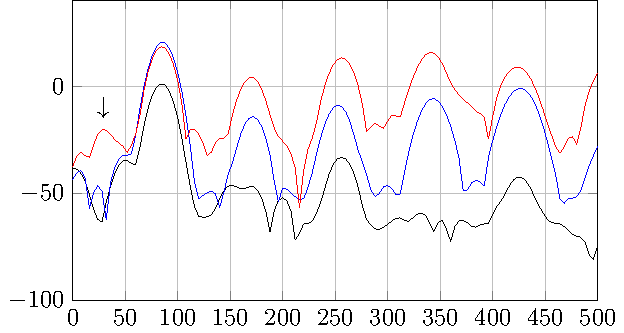
\includegraphics[width=0.6\textwidth]{FFT_hit}
%\end{figure}
%\begin{itemize}
%\item Sort: 0.005 Watt (81 dB SPL)
%\item Blå:  22 Watt (100 dB SPL)
%\item Rød:  294 Watt (105 dB SPL)
%
%\end{itemize}
%\end{frame}
%
%
%\subsection{Problemerne}
%\begin{frame}{Feedback system}{Problemerne}
%Følgende problemer ved feedback systemet:
%\begin{itemize}
%\item For dårlige sensorer
%\begin{itemize}
%\item Ikke præcise
%\item For meget støj
%\item For dyrer 
%\item Fejlmålinger
%\end{itemize}
%\item Ingen tendenser at spotte indtil et slag ramte = for sent
%\begin{itemize}
%\item Feedback tager for lang tid
%\end{itemize}
%\item Upraktisk at måle harmoniske toner 
%\begin{itemize}
%\item Ingen superpositions muligheder
%\item Fasen på signalerne passer ikke nødvendigvis
%\end{itemize}
%\end{itemize}
%\end{frame}
%
%%%%%%%%%%%%%%%%%
%
%\section{Feedforward system}
%
%\begin{frame}{Feedforward system}{Konceptet}
%
%\begin{figure}
%\centering
%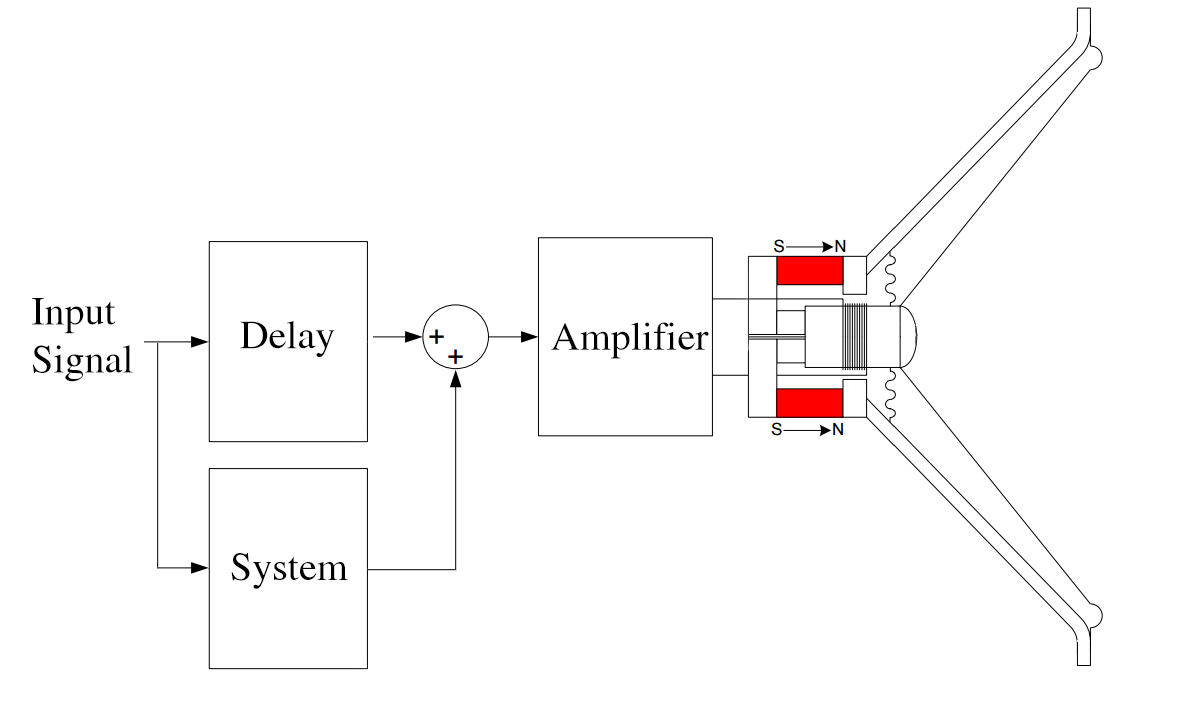
\includegraphics[width=0.9\textwidth]{Feedforward_Acc2}
%\end{figure}
%
%\end{frame}
%
%\begin{frame}{Feedforward system}{Overview}
%
%\begin{columns}
%  \begin{column}{0.70\textwidth}
%\begin{figure}
%\centering
%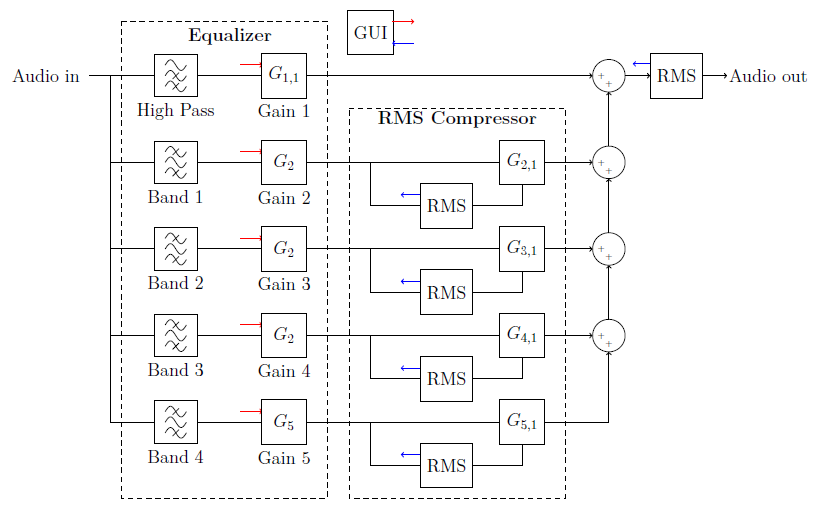
\includegraphics[width=0.85\textwidth]{Mainsystemoverview}
%\end{figure}
%  \end{column}
%  \begin{column}{0.30\textwidth}
%  \textbf{Systemet Overordnet}
%\begin{itemize}
%\item Grafisk Equalizer
%\item 4 Bånd i Bassen
%\begin{enumerate}
%\item 0   -   66 Hz
%\item 66  -  132 Hz
%\item 132 -  265 Hz
%\item 265 -  530 Hz
%\end{enumerate}
%\item RMS kompressor i 4 bånd
%\item RMS/Peak Limiter
%\item GUI til løbende justering
%\end{itemize}
%  \end{column}
%\end{columns}
%\end{frame}
%
%\subsection{Design Overvejelser}
%\begin{frame}{Feedforward system}{Design Overvejelser}
%\begin{columns}[t]
%  \begin{column}{0.50\textwidth}
%\textbf{Systemet skal:}
%\begin{itemize}
%\item Fungere ved lave frekvenser
%\item Have bånd til at måle frekvensområder
%\item Lineær fase
%\end{itemize}
%  \end{column}
%  \begin{column}{0.50\textwidth}
%  \textbf{Opnåes ved:}
%\begin{itemize}
%\item Realiseres som multi-rate
%\item Spektral subtraktion til at lave båndpas
%\item Opbygges af FIR filter
%\end{itemize}
%  \end{column}
%\end{columns}
%\vspace{5mm}
%\begin{block}{Overordnet set:}
%\begin{itemize}
%\item Downsampling til center frekvens på 3 kHz ved et 50-tap FIR filter
%\item x2 Downsampling 7 gange (x4,x8,x16,x32,x64)
%\item Indivudel kompressor i fire nederste bånd
%\end{itemize}
%\end{block}
%\end{frame}
%
%
%
%
%\subsection{Overordnet system}
%\begin{frame}{Feedforward system}{Systemet}
%
%\begin{columns}
%  \begin{column}{0.75\textwidth}
%\begin{figure}
%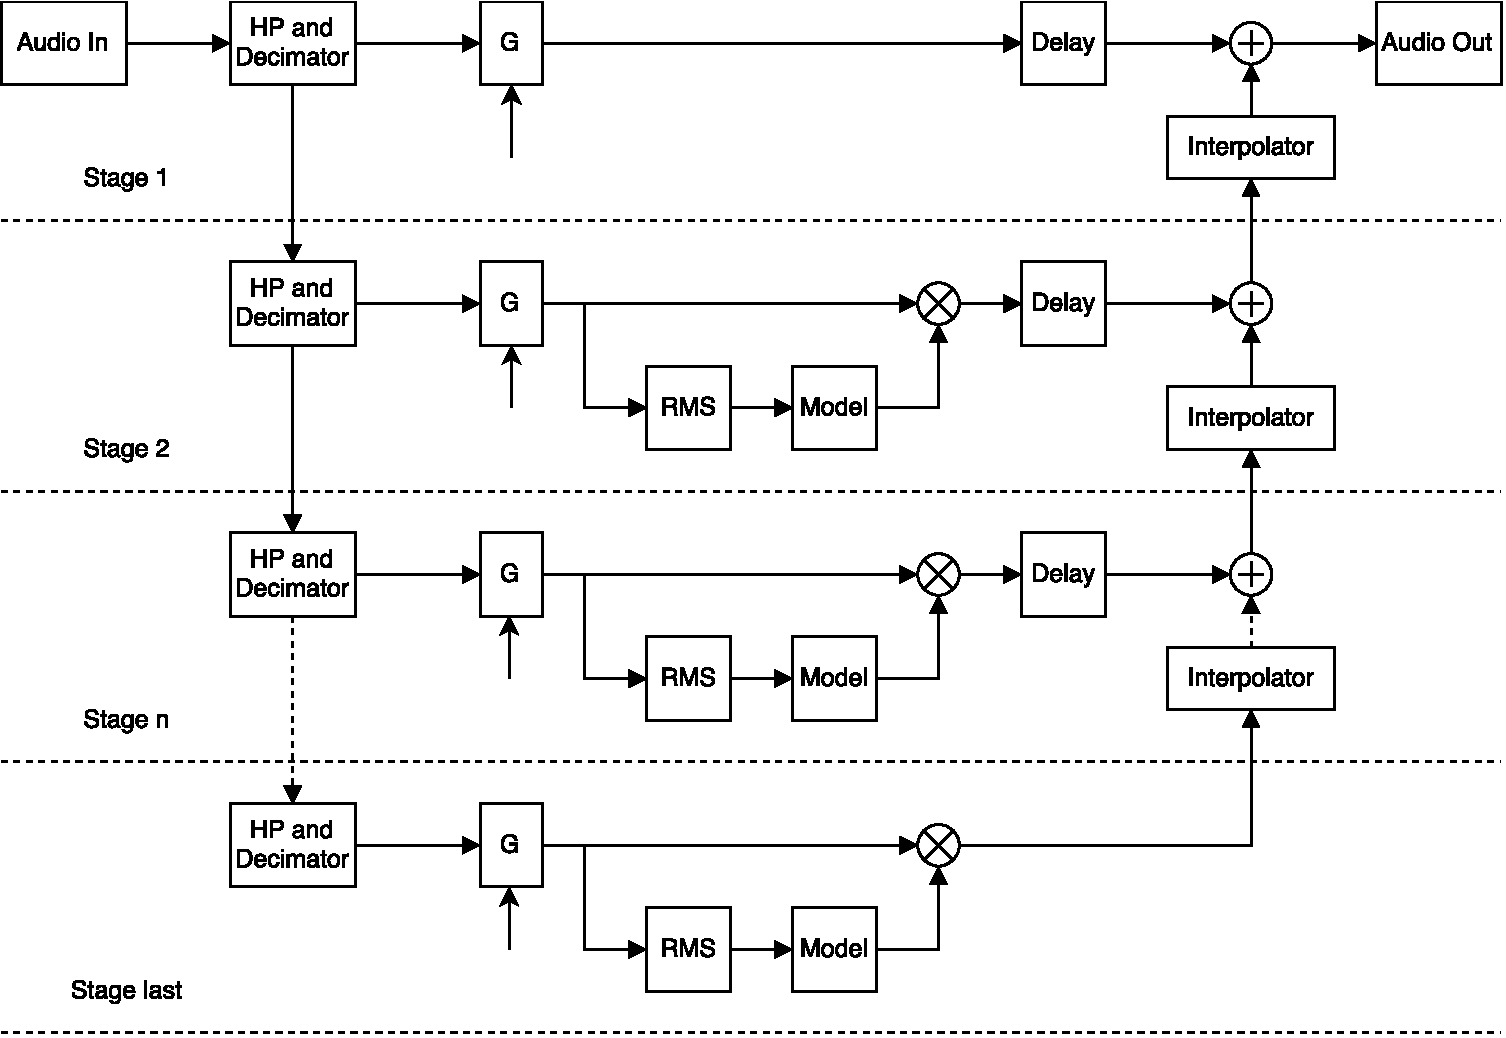
\includegraphics[width=\textwidth]{designRealBlock1}
%\end{figure}
%  \end{column}
%
%  \begin{column}{0.25\textwidth}
%  \textbf{Flow gennem system:}
%     \begin{enumerate}
%        \item Sample
%        \item Decimate
%        \item Spektral inversion
%        \item Påfør gain
%        \item Mål RMS
%        \item Påfør dæmpning
%        \item Interpolate
%        \item Summation
%     \end{enumerate}
%  \end{column}
%\end{columns}
%\end{frame}
%
%
%
%\subsection{Decimation}
%\begin{frame}{Feedforward system}{Decimator}
%
%\begin{columns}
%  \begin{column}{0.4\textwidth}
%\begin{figure}
%\centering
%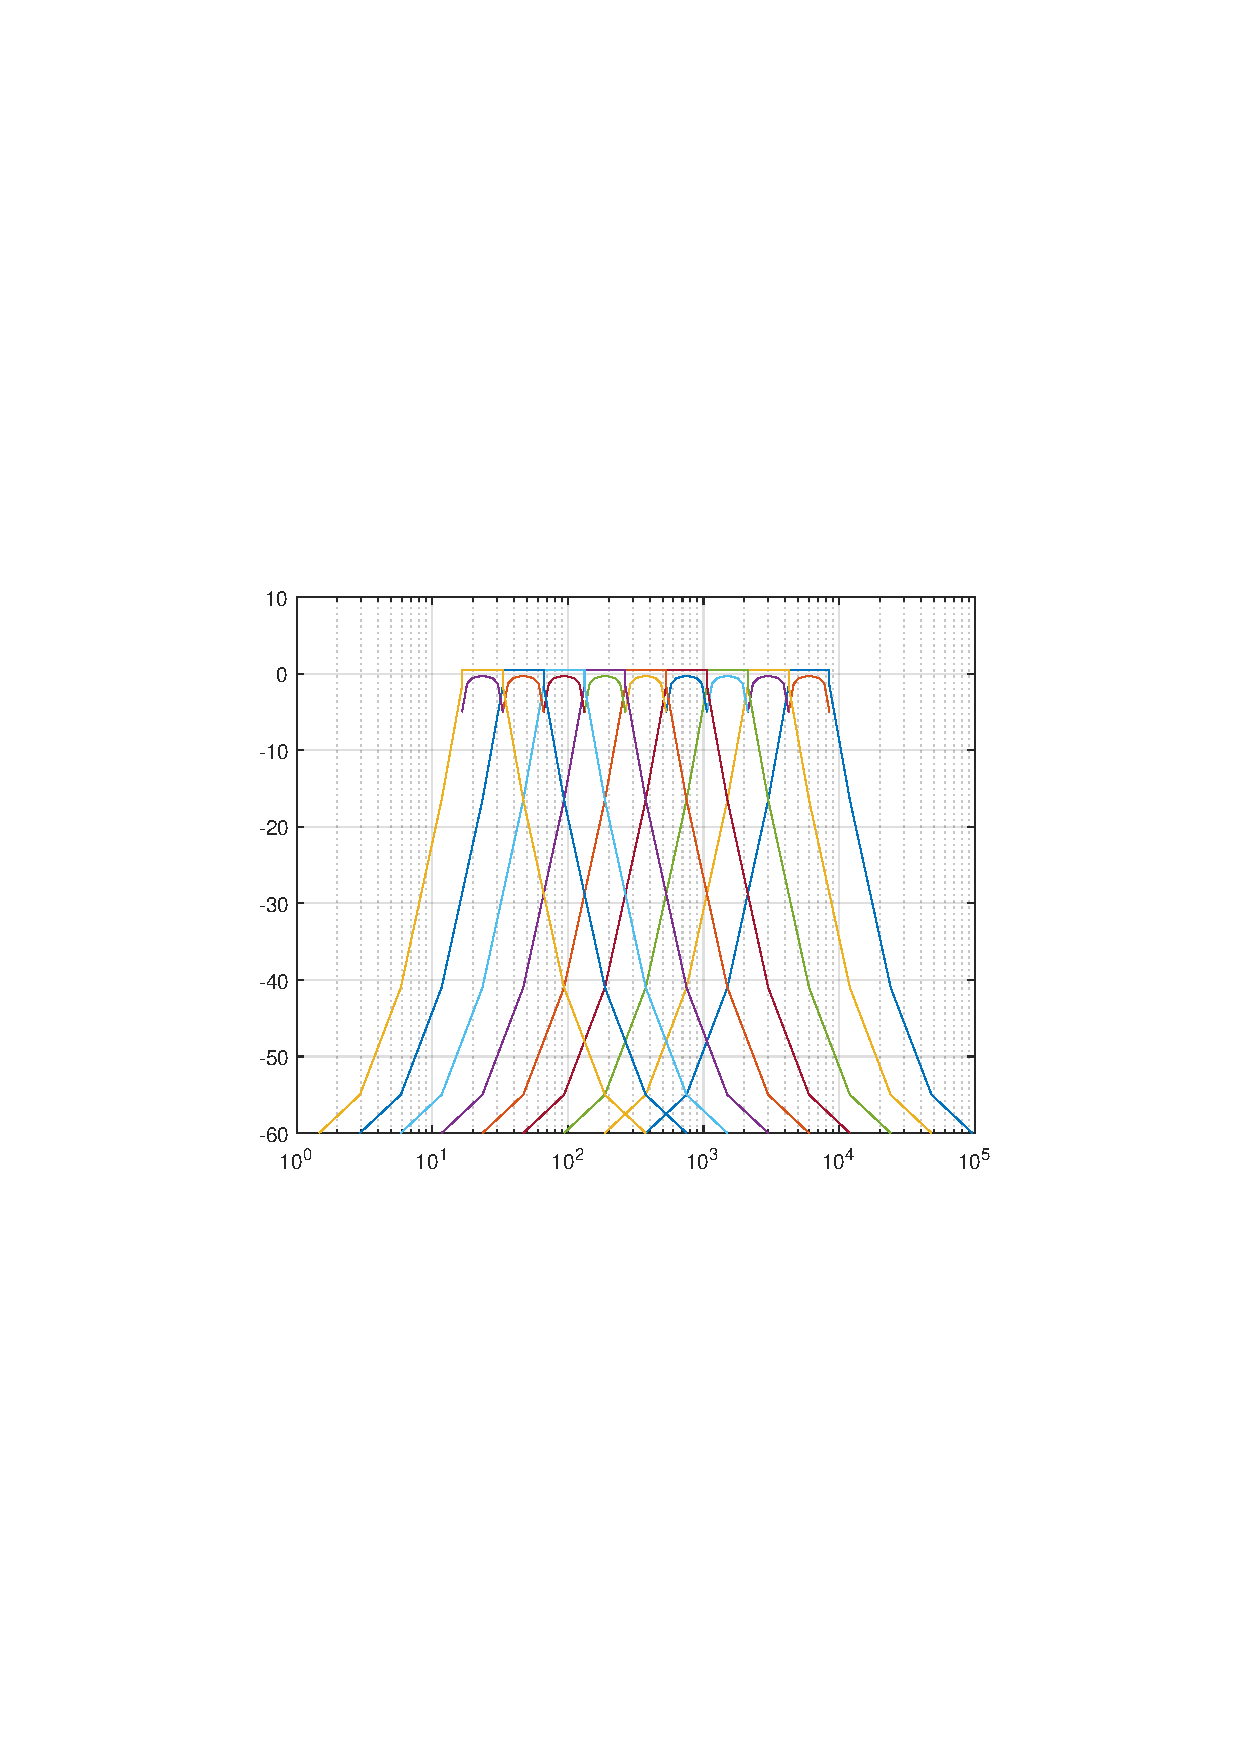
\includegraphics[width=\textwidth]{Bands}
%\end{figure}
%  \end{column}
%
%  \begin{column}{0.6\textwidth}
%\begin{itemize}
%\item 1 lavpas filter til båndpas
%\begin{itemize}
%\item Spektral subtraktion
%\end{itemize}
%\item 50. orden FIR
%\item Overholder IEC 6964 - Class 2 
%\end{itemize}
%\begin{figure}
%\centering
%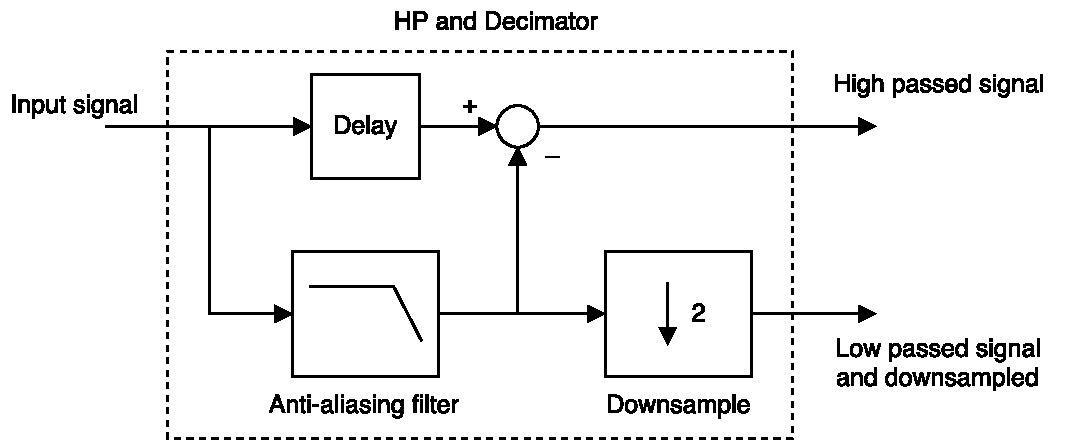
\includegraphics[width=\textwidth]{designRealDecimator}
%\end{figure}
%  \end{column}
%\end{columns}
%\end{frame}
%%%%%%%%%%%%%%%%%
%
%
%
%\subsection{RMS Compressor}
%\begin{frame}{Feedforward system}{RMS Compressor}
%
%\begin{columns}
%  \begin{column}{0.5\textwidth}
%\begin{figure}
%\centering
%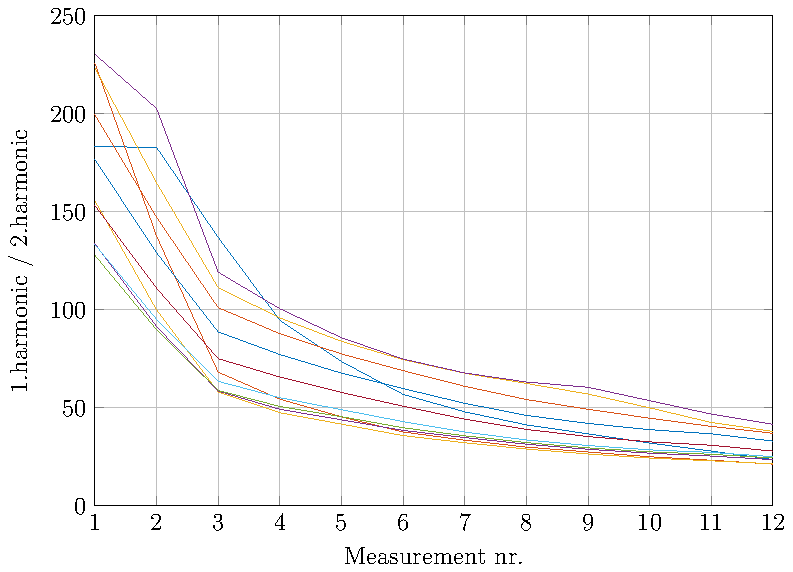
\includegraphics[width=0.7\textwidth]{comp_mic12All}
%\end{figure}
%\vspace{-5mm}
%\begin{figure}
%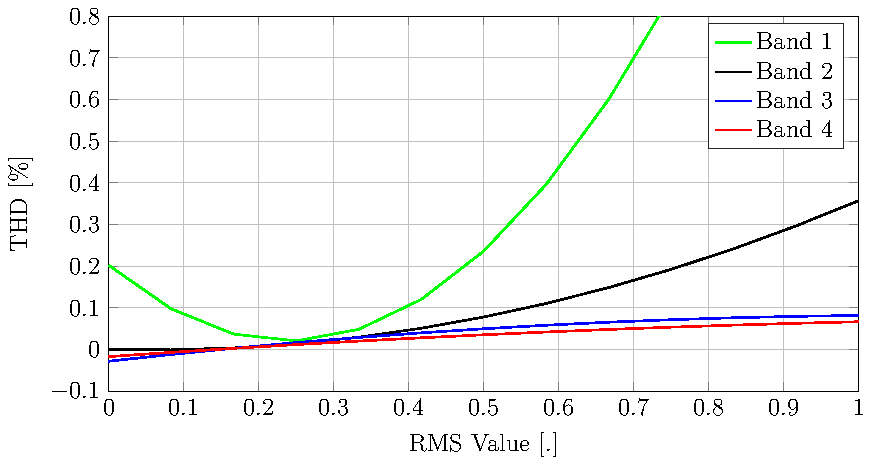
\includegraphics[width=0.8\textwidth]{BandModelCombine}
%\end{figure}
%  \end{column}
%  \begin{column}{0.5\textwidth}
%\begin{itemize}
%\item Dæmpning på op til 60 dB
%\item Opløsning på 1024 Steps
%\item Udskiftelig modeller
%\end{itemize}
%\begin{figure}
%\centering
%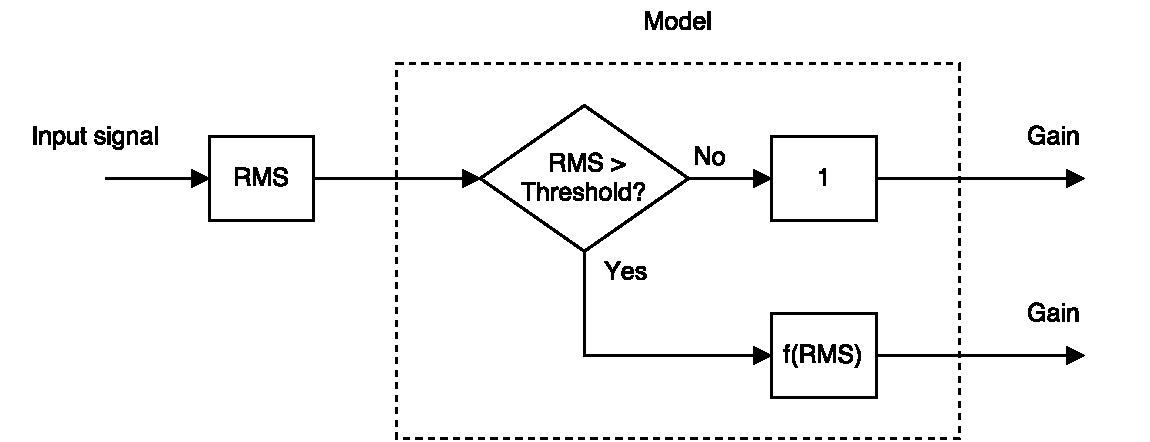
\includegraphics[width=\textwidth]{designRealRMS}
%\end{figure}
%  \end{column}
%\end{columns}
%
%\end{frame}
%
%
%
%
%\subsection{Interpolation}
%\begin{frame}{Feedforward system}{Interpolation}
%
%\begin{columns}
%  \begin{column}{0.4\textwidth}
%%\begin{figure}
%%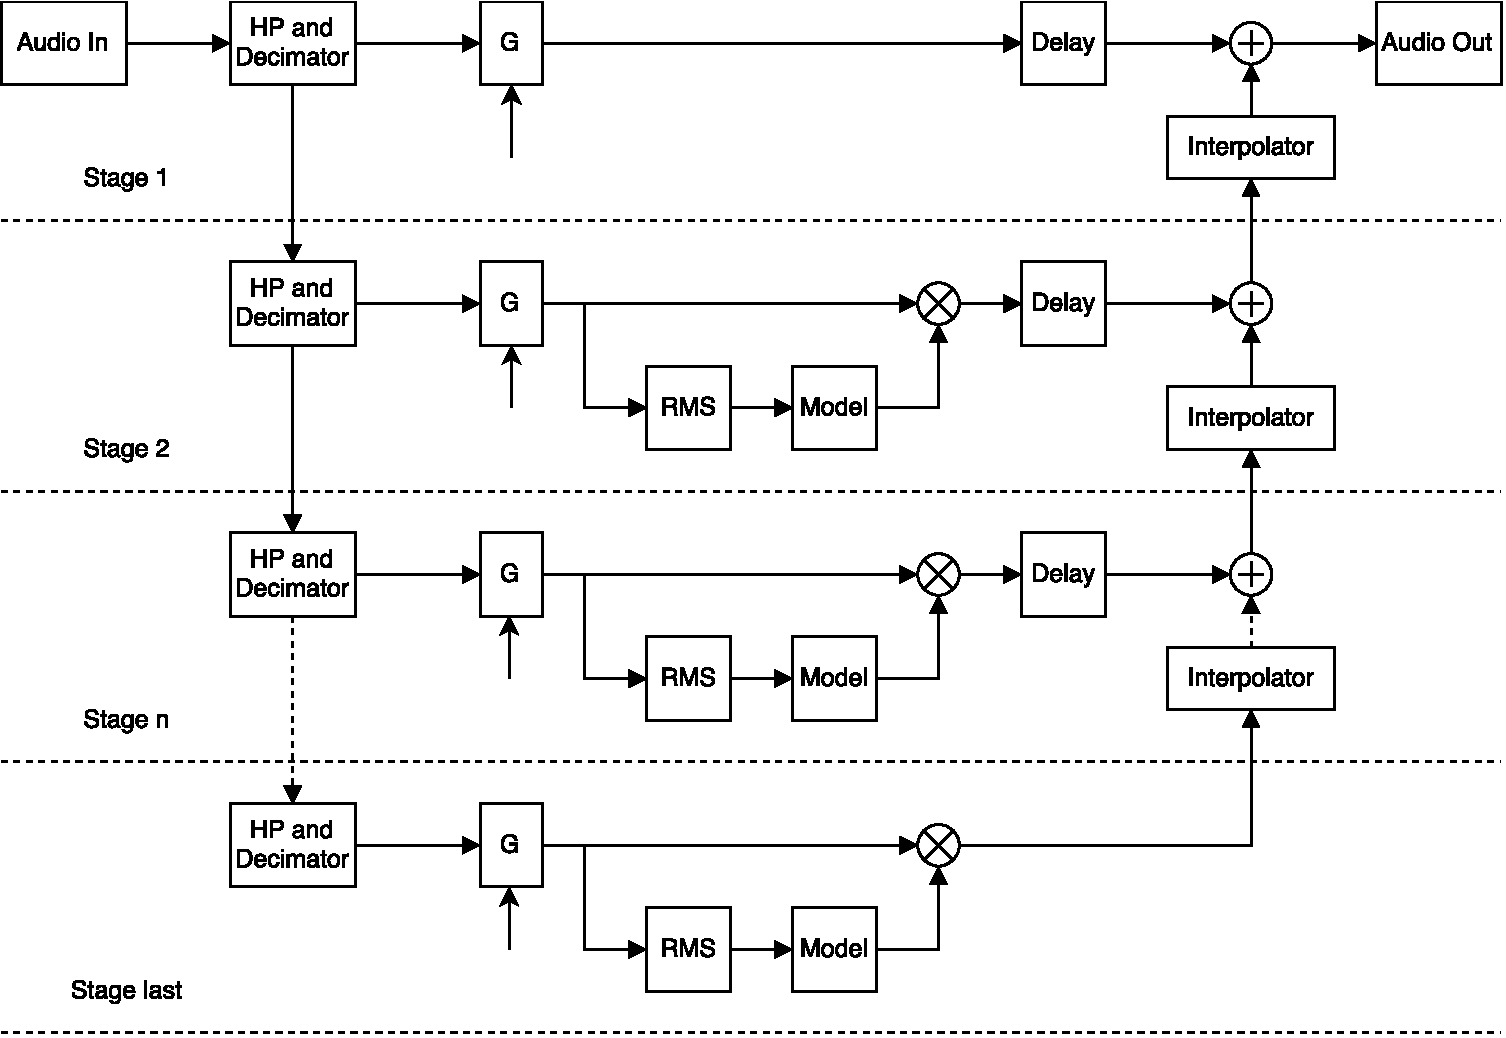
\includegraphics[width=0.9\textwidth]{designRealBlock1}
%%\end{figure}
%\begin{itemize}
%\item Zero-padding
%\item 48. Orden FIR
%\item Gain x2
%\end{itemize}
%  \end{column}
%
%  \begin{column}{0.6\textwidth}
%\begin{figure}
%\centering
%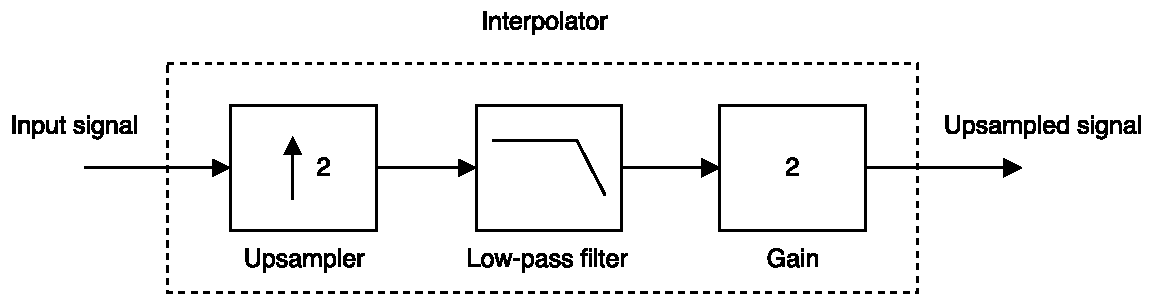
\includegraphics[width=\textwidth]{designRealInterpolator}
%\end{figure}
%  \end{column}
%\end{columns}
%
%\end{frame}
%
%
%
%\subsection{Simulering}
%\begin{frame}{Feedforward system}{Simulering}
%
%\begin{center}
%Simulering i MATLAB
%\end{center}
%
%\end{frame}
%
%\subsection{Opsumering}
%\begin{frame}{Feedforward system}{Opsumering}
%
%\begin{columns}[t]
%\begin{column}{0.40\textwidth}
%\textbf{Decimation/Interpolation:}
%\begin{itemize}
%\item Få instruktioner / Lav orden
%\item Billige FIR filter
%\item Mulighed for mere optimering
%\end{itemize}
%  \end{column}
%  \begin{column}{0.3\textwidth}
%\textbf{RMS Compressor:}
%\begin{itemize}
%\item Fleksible modeller
%\item Minimere hård limitering
%\item Fungere som både Peak og RMS
%\end{itemize}
%  \end{column}
%    \begin{column}{0.3\textwidth}
%\textbf{Overall:}
%\begin{itemize}
%\item Ingen støj
%\item Flat respons (+/- 1 dB)
%\end{itemize}
%  \end{column}
%\end{columns}
%
%\begin{block}{Kan Realiseres med:}
%\begin{itemize}
%\item Mulighed for 32-bit og 192 kHz
%\begin{itemize}
%\item Kun en ALU brugt
%\item 192 kHz vil kræve (x128,x256)
%\end{itemize}
%\end{itemize}
%\end{block}
%\vspace{-3mm}
%\begin{block}{Er Realiseret med:}
%\begin{itemize}
%\item Ca. 800 instruktioner.
%\item 16-bit og 48 kHz
%\item Peak limiter, RMS compressor og grafisk equalizer.
%\end{itemize}
%\end{block}
%
%\end{frame}
%
%
%\section{Demonstration}
%\begin{frame}{Feedforward system}{DEMO}
%
%\begin{center}
%DEMO\\
%\textit{Med forbehold}
%\end{center}
%\end{frame}
%
%\section{Spørgsmål og Evt.}
%% contact information
%\begin{frame}{Spørgsmål og Evt.}
%  \begin{center}
%Spørgsmål og Evt.
%  \end{center}
%\end{frame}

%\section{Optimering}
%\begin{frame}{Optimering}{Poul Hoang}
%
%\end{frame}

\subsection{Relevante optimerings muligheder}
\begin{frame}{Optimering}{Relevante optimerings muligheder}
	\begin{itemize}
\item Reducering af anvendte instruktioner.
\begin{itemize}
	\item Gennemsnitligt 900 instruktioner pr. sample.
	\begin{enumerate}
		\item Generel optimering såsom cirkulære buffer og DUAL-MAC
		\item Polyphase FIR filtre
	\end{enumerate}
\end{itemize}

\item Mindre delay gennem systemet
\begin{itemize}
	\item 111 ms delay gennem systemet
	\begin{enumerate}
		\item Færre trin/bånd (stages) i systemet
		\item IIR filter i interpolation
	\end{enumerate}
\end{itemize}
\item Bedre RMS limiter 
	\end{itemize}
\end{frame}

\begin{frame}{Optimering}{Reducering af anvendte instruktioner}
Generel reducering af anvendte instruktioner
\begin{itemize}
\item Dobbelt initialisering af buffere. (30 – 40 instruktioner) 
\item Reservering af cirkulære buffere
\begin{itemize}
\item TMS320C5515 kan initialisere fem cirkulære buffere
\item Fire kan reseveres til udvalgte filtre
\item Færre instruktioner på initialisering (10 - 20 instruktioner)
\end{itemize}
\item Færre funktionskald
\item Multirate algoritme til schedulering frigør program memory
\end{itemize}
\end{frame}


\begin{frame}{Optimering}{Reducering af anvendte instruktioner}
Zero-padding anvendes i interpolation\\
\vspace{5mm}
Halvdelen af udregningerne giver nul\\
\vspace{5mm}
Polyphase filter i interpolation halvere filter algoritmen
\begin{figure}[H]
\centering
\includegraphics[width=0.6\textwidth]{polyFilter}
\end{figure}
\end{frame}

\begin{frame}{Optimering}{Mindre delay gennem systemet}
Færre trin/bånd (stages) i systemet \\
\vspace{5mm}
IIR filter i interpolation
\begin{itemize}
\item Mindre delay
\item Lille ulinearitet ved signalbåndbredde
\end{itemize}
\end{frame}

\begin{frame}{Optimering}{Mindre delay gennem systemet}
Butterworth IIR filter
\begin{itemize}
\item N = 8
\item Cutoff = 0.5$\pi$
\end{itemize}
\begin{columns}
\begin{column}{0.45\textwidth}
\begin{figure}[H]
\centering
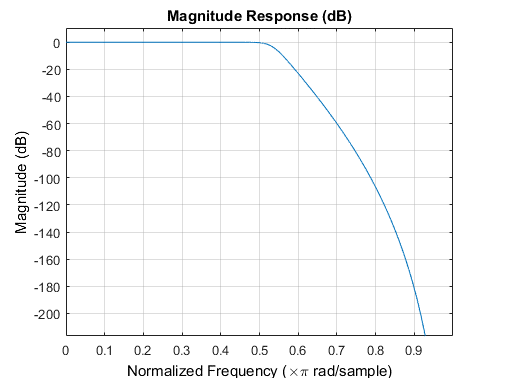
\includegraphics[width=0.9\textwidth]{IIRFrekvens}
\end{figure}
\end{column}
\begin{column}{0.45\textwidth}
\begin{figure}[H]
\centering
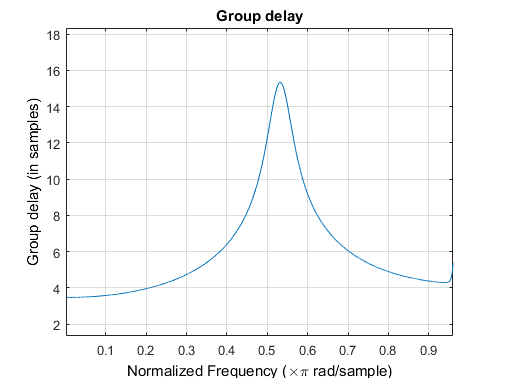
\includegraphics[width=0.9\textwidth]{IIRdelay}
\end{figure}
\end{column}
\end{columns}
\end{frame}

\begin{frame}{Optimering}{Optimeret RMS limiter design}
Delay i RMS limiter design for at beskytte mod transiente signaler
\begin{figure}[H]
\centering
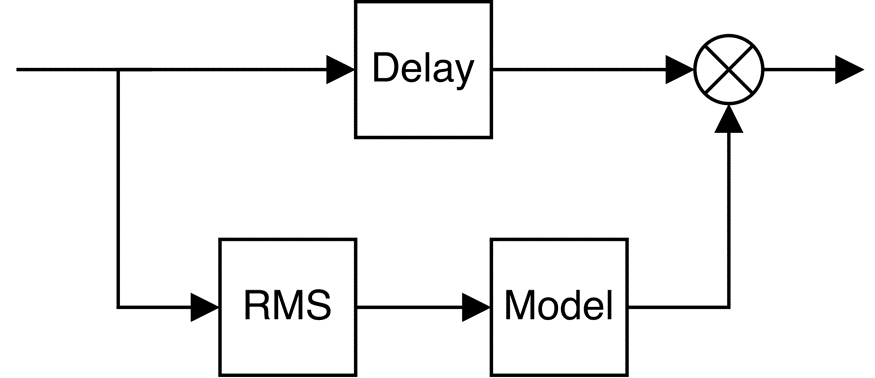
\includegraphics[width=0.6\textwidth]{RMSoptimering}
\end{figure}
\end{frame}

\section{Perspektivering}
\begin{frame}{Perspektivering}{Perspektivering/Konklusion}
Systemet er velegnet til mindre højttalere \\
\begin{itemize}
\item Mere effekt kan afsættes uden at ødelægge wooferen
\end{itemize}	
\vspace{5mm}
Forstærkningen for en aktiv højtaler kan øges \\
\begin{itemize}
\item Systemet sørger for at bassen holdes under en threshold
\end{itemize}	
\end{frame}

\section{Diskussion og afsluttende ord}
\begin{frame}{Diskussion og afsluttende ord}
Projekt uden konkrete fortilfælde \\
\vspace{5mm}
Projektet har undersøgt både feedback og feedforward som løsning \\
\vspace{5mm}
Størstedelen af projektet har været konceptudvikling \\
\vspace{5mm}
Projektet omhandler en aktuel problemstilling
\end{frame}


\section{Demonstration}
\begin{frame}{Demonstration}
	Lad os alle gå mod lab
\end{frame}

%\section{Introduktion}
%% motivation for creating this theme
%\begin{frame}{Introduktion}{}
%  Målet med dette projekt er at:
%  \begin{itemize}
%    \item Beskytte bas enhederne
%    \begin{itemize}
%    \item Begrænse slag mod bagpladen
%\end{itemize}
%\item Minimal komprimering/limitering       
%  \end{itemize}
%  \vspace{5mm}
%  Samtidigt med at følgende krav kunne realiseres:
%  \begin{itemize}
%  	\item Mindre end 1024 Instruktioner pr. sample
%  	\item Mulighed for sampling rate på 96 kHz
%  	\item Mulighed for at køre med 24-Bit
%  \end{itemize}
%\end{frame}
%%%%%%%%%%%%%%%%%
%
%\section{Feedback system}
%% the license
%\begin{frame}{Feedback system}{Første antagelse}
%\begin{figure}[t]
%\centering
%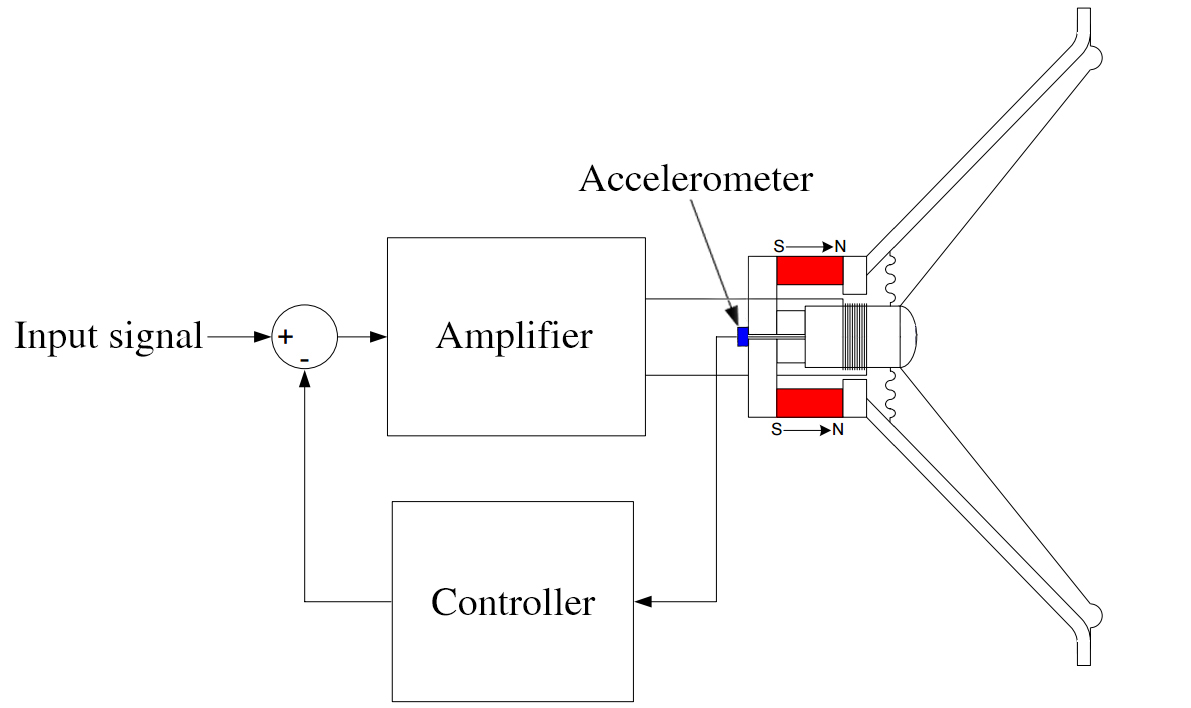
\includegraphics[width=0.75\textwidth]{Feedback_Acc2}
%\end{figure}
%\end{frame}
%
%\subsection{Analyse}
%\begin{frame}{Feedback system}{Analyse}
%Lineært sweep fra 2400 til 0 Hz
%\begin{figure}
%\centering
%\begin{subfigure}[t]{0.45\textwidth}
%\centering
%%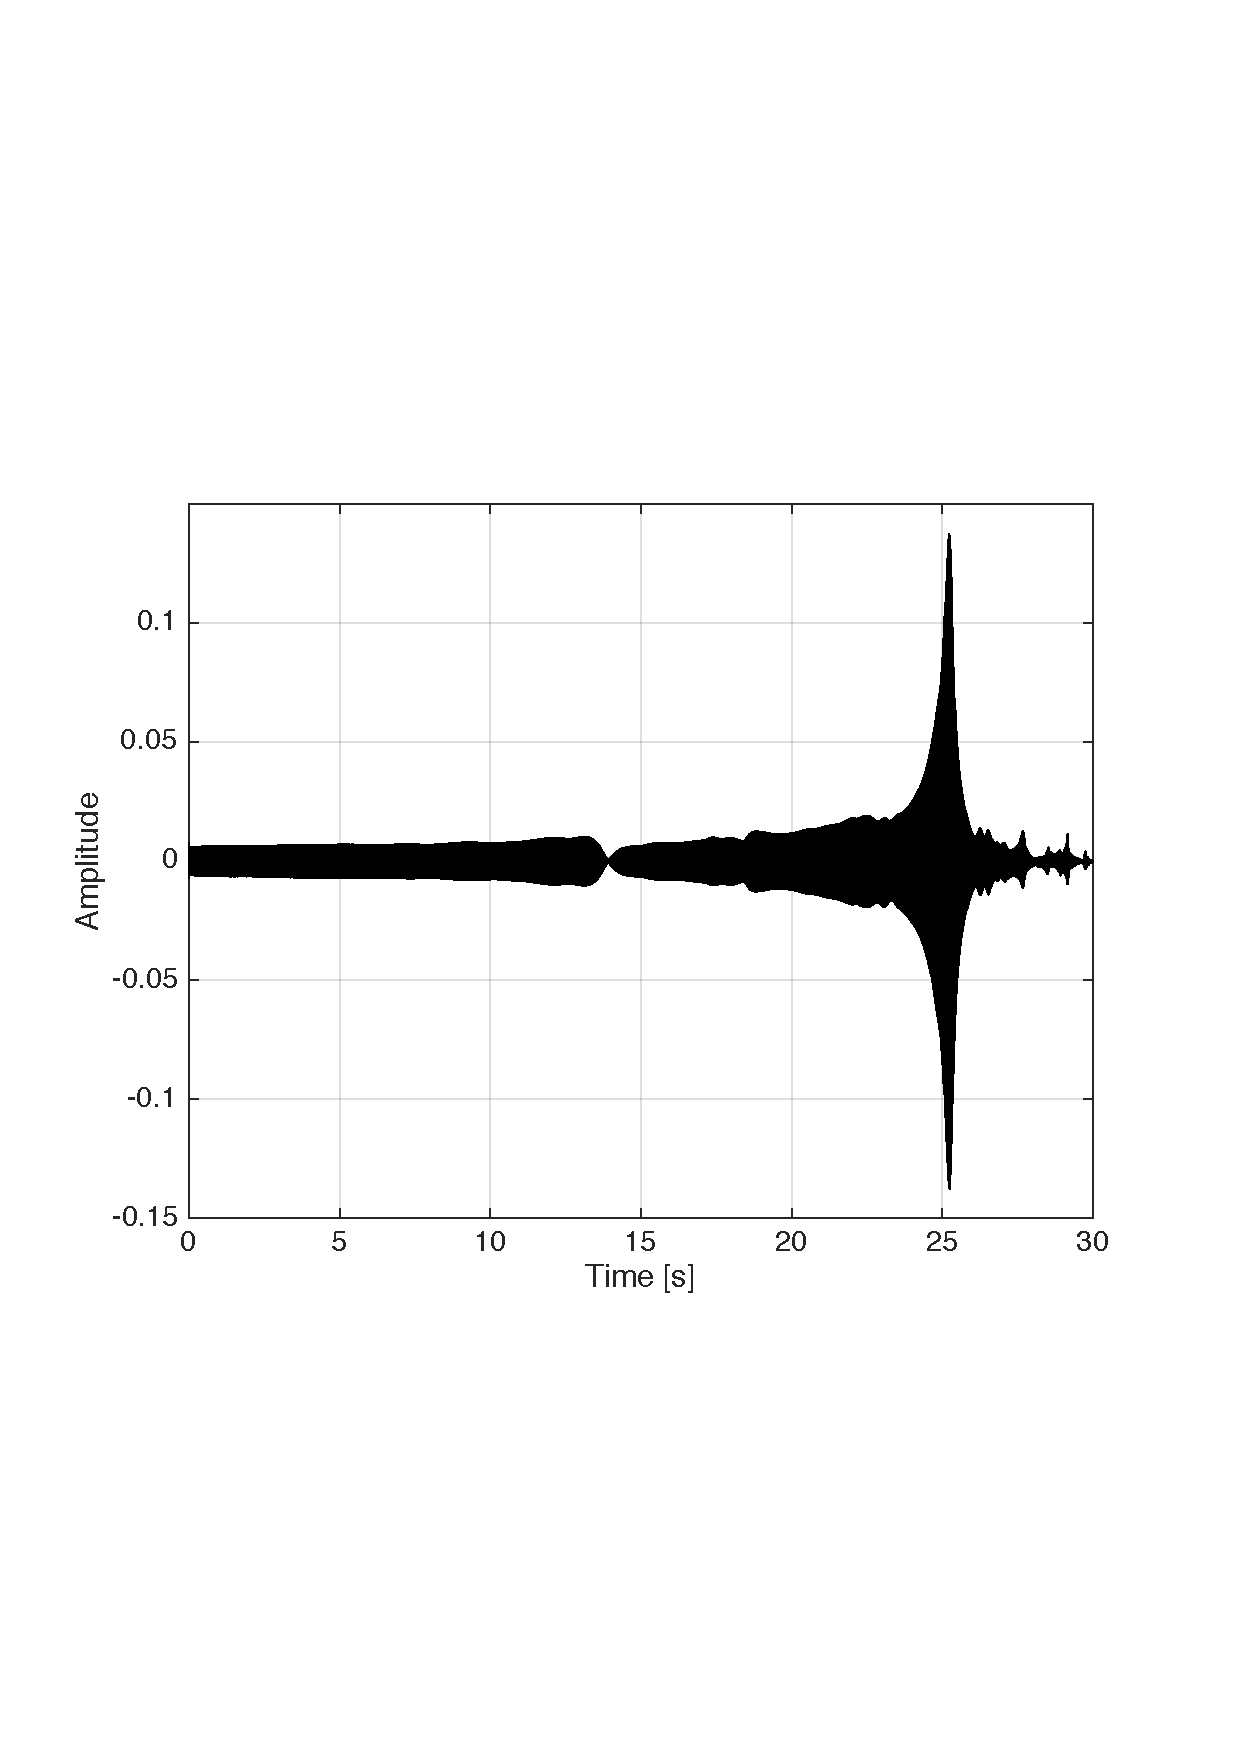
\includegraphics[width=\textwidth]{raw_driver10}
%% This file was created by matlab2tikz.
%
%The latest updates can be retrieved from
%  http://www.mathworks.com/matlabcentral/fileexchange/22022-matlab2tikz-matlab2tikz
%where you can also make suggestions and rate matlab2tikz.
%
\begin{tikzpicture}

\begin{axis}[%
width=5.521in,
height=2in,
at={(0.758in,0.481in)},
xmin=0,
xmax=30,
xmajorgrids,
ymin=-0.15,
ymax=0.15,
ymajorgrids,
axis background/.style={fill=white}
]
\addplot[fill=black,draw=black,forget plot] plot table[row sep=crcr]{%
2.08333333333333e-05	0.0119891166687012\\
0.0425739952718676	0.0120701789855957\\
0.0851271572104019	0.0120600461959839\\
0.127680319148936	0.0121411085128784\\
0.17023348108747	0.0122112035751343\\
0.212786643026005	0.0122820138931274\\
0.255339804964539	0.0123153924942017\\
0.297892966903073	0.0123672485351563\\
0.340446128841608	0.0123822689056396\\
0.382999290780142	0.0124343633651733\\
0.425552452718676	0.012420654296875\\
0.46810561465721	0.0124455690383911\\
0.510658776595745	0.0124385356903076\\
0.553211938534279	0.0124293565750122\\
0.595765100472813	0.0124131441116333\\
0.638318262411347	0.0123996734619141\\
0.680871424349882	0.0123659372329712\\
0.723424586288416	0.0123772621154785\\
0.76597774822695	0.0123530626296997\\
0.808530910165485	0.0123927593231201\\
0.851084072104019	0.0123993158340454\\
0.893637234042553	0.0123468637466431\\
0.936190395981088	0.0123317241668701\\
0.978743557919622	0.0123351812362671\\
1.02129671985816	0.0123213529586792\\
1.06384988179669	0.012315034866333\\
1.10640304373522	0.0123295783996582\\
1.14895620567376	0.0123213529586792\\
1.19150936761229	0.012312650680542\\
1.23406252955083	0.0123451948165894\\
1.27661569148936	0.0123229026794434\\
1.3191688534279	0.0123435258865356\\
1.36172201536643	0.0123484134674072\\
1.40427517730496	0.0123796463012695\\
1.4468283392435	0.0123721361160278\\
1.48938150118203	0.0123879909515381\\
1.53193466312057	0.012427806854248\\
1.5744878250591	0.0124756097793579\\
1.61704098699764	0.012513279914856\\
1.65959414893617	0.0124995708465576\\
1.7021473108747	0.0125466585159302\\
1.74470047281324	0.012596607208252\\
1.78725363475177	0.0126116275787354\\
1.82980679669031	0.0126550197601318\\
1.87235995862884	0.012694239616394\\
1.91491312056738	0.0127073526382446\\
1.95746628250591	0.0127198696136475\\
2.00001944444444	0.0127586126327515\\
2.04257260638298	0.0127676725387573\\
2.08512576832151	0.012792706489563\\
2.12767893026005	0.0128316879272461\\
2.17023209219858	0.0128744840621948\\
2.21278525413712	0.0128858089447021\\
2.25533841607565	0.0128728151321411\\
2.29789157801418	0.0128904581069946\\
2.34044473995272	0.012937068939209\\
2.38299790189125	0.0129625797271729\\
2.42555106382979	0.0129508972167969\\
2.46810422576832	0.0129650831222534\\
2.51065738770686	0.0130186080932617\\
2.55321054964539	0.0130044221878052\\
2.59576371158392	0.0130490064620972\\
2.63831687352246	0.0130782127380371\\
2.68087003546099	0.0130912065505981\\
2.72342319739953	0.0131031274795532\\
2.76597635933806	0.0131406784057617\\
2.8085295212766	0.0131857395172119\\
2.85108268321513	0.0132355690002441\\
2.89363584515366	0.0132455825805664\\
2.9361890070922	0.0132309198379517\\
2.97874216903073	0.013269305229187\\
3.02129533096927	0.0133043527603149\\
3.0638484929078	0.013329029083252\\
3.10640165484634	0.0133227109909058\\
3.14895481678487	0.0133368968963623\\
3.1915079787234	0.0133442878723145\\
3.23406114066194	0.0133599042892456\\
3.27661430260047	0.0133839845657349\\
3.31916746453901	0.0133798122406006\\
3.36172062647754	0.0133849382400513\\
3.40427378841608	0.0134093761444092\\
3.44682695035461	0.013446569442749\\
3.48938011229314	0.0134661197662354\\
3.53193327423168	0.0134836435317993\\
3.57448643617021	0.013521671295166\\
3.61703959810875	0.0135370492935181\\
3.65959276004728	0.0135470628738403\\
3.70214592198582	0.0135759115219116\\
3.74469908392435	0.0136080980300903\\
3.78725224586288	0.0136371850967407\\
3.82980540780142	0.0136731863021851\\
3.87235856973995	0.0137186050415039\\
3.91491173167849	0.0137549638748169\\
3.95746489361702	0.0137441158294678\\
4.00001805555556	0.0138174295425415\\
4.04257121749409	0.013864278793335\\
4.08512437943262	0.0139147043228149\\
4.12767754137116	0.0139368772506714\\
4.17023070330969	0.0140061378479004\\
4.21278386524823	0.0140299797058105\\
4.25533702718676	0.0140790939331055\\
4.29789018912529	0.0141112804412842\\
4.34044335106383	0.0141588449478149\\
4.38299651300236	0.0141901969909668\\
4.4255496749409	0.0142172574996948\\
4.46810283687943	0.0142718553543091\\
4.51065599881797	0.0143095254898071\\
4.5532091607565	0.0143332481384277\\
4.59576232269503	0.0143661499023438\\
4.63831548463357	0.0144078731536865\\
4.6808686465721	0.0144317150115967\\
4.72342180851064	0.014464259147644\\
4.76597497044917	0.0144739151000977\\
4.80852813238771	0.0144917964935303\\
4.85108129432624	0.0145350694656372\\
4.89363445626477	0.0145490169525146\\
4.93618761820331	0.014581561088562\\
4.97874078014184	0.0145977735519409\\
5.02129394208038	0.0146069526672363\\
5.06384710401891	0.0146232843399048\\
5.10640026595745	0.0146393775939941\\
5.14895342789598	0.0146942138671875\\
5.19150658983452	0.0146994590759277\\
5.23405975177305	0.0147175788879395\\
5.27661291371158	0.0147092342376709\\
5.31916607565012	0.0147404670715332\\
5.36171923758865	0.0147354602813721\\
5.40427239952719	0.0147433280944824\\
5.44682556146572	0.0147520303726196\\
5.48937872340426	0.0147508382797241\\
5.53193188534279	0.0147504806518555\\
5.57448504728132	0.014761209487915\\
5.61703820921986	0.0147466659545898\\
5.65959137115839	0.0147426128387451\\
5.70214453309693	0.0147403478622437\\
5.74469769503546	0.0147124528884888\\
5.787250856974	0.0147058963775635\\
5.82980401891253	0.0147024393081665\\
5.87235718085106	0.0146327018737793\\
5.9149103427896	0.0146118402481079\\
5.95746350472813	0.0145947933197021\\
6.00001666666667	0.0145722627639771\\
6.0425698286052	0.0145455598831177\\
6.08512299054374	0.0144891738891602\\
6.12767615248227	0.0144437551498413\\
6.1702293144208	0.0144070386886597\\
6.21278247635934	0.014379620552063\\
6.25533563829787	0.0143579244613647\\
6.29788880023641	0.0142805576324463\\
6.34044196217494	0.0142168998718262\\
6.38299512411347	0.014191746711731\\
6.42554828605201	0.0140836238861084\\
6.46810144799054	0.0140348672866821\\
6.51065460992908	0.0139898061752319\\
6.55320777186761	0.0139384269714355\\
6.59576093380615	0.0138537883758545\\
6.63831409574468	0.0137983560562134\\
6.68086725768321	0.0137511491775513\\
6.72342041962175	0.0137094259262085\\
6.76597358156028	0.0136710405349731\\
6.80852674349882	0.0136563777923584\\
6.85107990543735	0.0136498212814331\\
6.89363306737589	0.0136363506317139\\
6.93618622931442	0.0136944055557251\\
6.97873939125296	0.0137603282928467\\
7.02129255319149	0.0138442516326904\\
7.06384571513002	0.0139046907424927\\
7.10639887706856	0.0139477252960205\\
7.14895203900709	0.014054536819458\\
7.19150520094563	0.0141353607177734\\
7.23405836288416	0.0142430067062378\\
7.27661152482269	0.0143053531646729\\
7.31916468676123	0.014385461807251\\
7.36171784869976	0.0145281553268433\\
7.4042710106383	0.0145792961120605\\
7.44682417257683	0.0146374702453613\\
7.48937733451537	0.014722466468811\\
7.5319304964539	0.0147558450698853\\
7.57448365839243	0.0148293972015381\\
7.61703682033097	0.0148519277572632\\
7.6595899822695	0.0148772001266479\\
7.70214314420804	0.0148836374282837\\
7.74469630614657	0.0149027109146118\\
7.78724946808511	0.0148898363113403\\
7.82980263002364	0.0149227380752563\\
7.87235579196217	0.0149306058883667\\
7.91490895390071	0.0149260759353638\\
7.95746211583924	0.0149365663528442\\
8.00001527777778	0.0149394273757935\\
8.04256843971631	0.0149445533752441\\
8.08512160165485	0.0149415731430054\\
8.12767476359338	0.0149654150009155\\
8.17022792553192	0.0149649381637573\\
8.21278108747045	0.014962911605835\\
8.25533424940898	0.0149157047271729\\
8.29788741134752	0.0148886442184448\\
8.34044057328605	0.0148481130599976\\
8.38299373522459	0.0147963762283325\\
8.42554689716312	0.0147671699523926\\
8.46810005910165	0.0147316455841064\\
8.51065322104019	0.0146907567977905\\
8.55320638297872	0.0146373510360718\\
8.59575954491726	0.0146878957748413\\
8.63831270685579	0.0146653652191162\\
8.68086586879433	0.0146582126617432\\
8.72341903073286	0.0146515369415283\\
8.76597219267139	0.0146892070770264\\
8.80852535460993	0.0147384405136108\\
8.85107851654846	0.0147976875305176\\
8.893631678487	0.0148004293441772\\
8.93618484042553	0.0149153470993042\\
8.97873800236407	0.0149699449539185\\
9.0212911643026	0.0150353908538818\\
9.06384432624114	0.0150772333145142\\
9.10639748817967	0.0151313543319702\\
9.1489506501182	0.0152260065078735\\
9.19150381205674	0.0153157711029053\\
9.23405697399527	0.015323281288147\\
9.27661013593381	0.0154021978378296\\
9.31916329787234	0.0154614448547363\\
9.36171645981088	0.0155340433120728\\
9.40426962174941	0.015607476234436\\
9.44682278368794	0.015711784362793\\
9.48937594562648	0.0157406330108643\\
9.53192910756501	0.0158414840698242\\
9.57448226950355	0.0159074068069458\\
9.61703543144208	0.0159391164779663\\
9.65958859338062	0.0160180330276489\\
9.70214175531915	0.0160245895385742\\
9.74469491725768	0.0160360336303711\\
9.78724807919622	0.01607346534729\\
9.82980124113475	0.0160551071166992\\
9.87235440307329	0.0160226821899414\\
9.91490756501182	0.0159975290298462\\
9.95746072695036	0.0159332752227783\\
10.0000138888889	0.0159041881561279\\
10.0425670508274	0.0158710479736328\\
10.085120212766	0.0158164501190186\\
10.1276733747045	0.0158092975616455\\
10.170226536643	0.0157977342605591\\
10.2127796985816	0.0158299207687378\\
10.2553328605201	0.0159136056900024\\
10.2978860224586	0.0159791707992554\\
10.3404391843972	0.016069769859314\\
10.3829923463357	0.0161577463150024\\
10.4255455082742	0.0162630081176758\\
10.4680986702128	0.0163758993148804\\
10.5106518321513	0.0164648294448853\\
10.5532049940898	0.0165594816207886\\
10.5957581560284	0.0166622400283813\\
10.6383113179669	0.016768217086792\\
10.6808644799054	0.0168865919113159\\
10.723417641844	0.0169931650161743\\
10.7659708037825	0.0171152353286743\\
10.808523965721	0.0171926021575928\\
10.8510771276596	0.017282247543335\\
10.8936302895981	0.0174212455749512\\
10.9361834515366	0.0175200700759888\\
10.9787366134752	0.0176385641098022\\
11.0212897754137	0.0177961587905884\\
11.0638429373522	0.0178617238998413\\
11.1063960992908	0.0179822444915771\\
11.1489492612293	0.0180516242980957\\
11.1915024231678	0.0181763172149658\\
11.2340555851064	0.0183032751083374\\
11.2766087470449	0.0184470415115356\\
11.3191619089835	0.0185744762420654\\
11.361715070922	0.0186715126037598\\
11.4042682328605	0.0187947750091553\\
11.4468213947991	0.0189191102981567\\
11.4893745567376	0.0189660787582397\\
11.5319277186761	0.0190688371658325\\
11.5744808806147	0.019160270690918\\
11.6170340425532	0.0192372798919678\\
11.6595872044917	0.0193090438842773\\
11.7021403664303	0.019400954246521\\
11.7446935283688	0.0195177793502808\\
11.7872466903073	0.0195590257644653\\
11.8297998522459	0.0196257829666138\\
11.8723530141844	0.0197001695632935\\
11.9149061761229	0.0197663307189941\\
11.9574593380615	0.0198649168014526\\
12.0000125	0.0199562311172485\\
12.0425656619385	0.0200393199920654\\
12.0851188238771	0.0201531648635864\\
12.1276719858156	0.0202683210372925\\
12.1702251477541	0.0203834772109985\\
12.2127783096927	0.0205181837081909\\
12.2553314716312	0.0206431150436401\\
12.2978846335697	0.020803689956665\\
12.3404377955083	0.0209430456161499\\
12.3829909574468	0.0210655927658081\\
12.4255441193853	0.0211613178253174\\
12.4680972813239	0.0213009119033813\\
12.5106504432624	0.0214111804962158\\
12.5532036052009	0.0215167999267578\\
12.5957567671395	0.0215667486190796\\
12.638309929078	0.0216765403747559\\
12.6808630910165	0.0217441320419312\\
12.7234162529551	0.0217874050140381\\
12.7659694148936	0.0218304395675659\\
12.8085225768322	0.0218579769134521\\
12.8510757387707	0.0218334197998047\\
12.8936289007092	0.0218534469604492\\
12.9361820626478	0.0217874050140381\\
12.9787352245863	0.0216927528381348\\
13.0212883865248	0.021544337272644\\
13.0638415484634	0.021371603012085\\
13.1063947104019	0.0211578607559204\\
13.1489478723404	0.0209262371063232\\
13.191501034279	0.0206685066223145\\
13.2340541962175	0.0203869342803955\\
13.276607358156	0.0200080871582031\\
13.3191605200946	0.019722580909729\\
13.3617136820331	0.0194058418273926\\
13.4042668439716	0.0190954208374023\\
13.4468200059102	0.0187587738037109\\
13.4893731678487	0.0184516906738281\\
13.5319263297872	0.0181584358215332\\
13.5744794917258	0.0178221464157104\\
13.6170326536643	0.0174729824066162\\
13.6595858156028	0.0171077251434326\\
13.7021389775414	0.016639232635498\\
13.7446921394799	0.0161151885986328\\
13.7872453014184	0.0154547691345215\\
13.829798463357	0.0146360397338867\\
13.8723516252955	0.0137324333190918\\
13.914904787234	0.0126259326934814\\
13.9574579491726	0.0113997459411621\\
14.0000111111111	0.0100481510162354\\
14.0425642730496	0.00874054431915283\\
14.0851174349882	0.00763881206512451\\
14.1276705969267	0.00698995590209961\\
14.1702237588652	0.00721240043640137\\
14.2127769208038	0.0078728199005127\\
14.2553300827423	0.00864839553833008\\
14.2978832446809	0.00943124294281006\\
14.3404364066194	0.010124683380127\\
14.3829895685579	0.0107450485229492\\
14.4255427304965	0.0112762451171875\\
14.468095892435	0.0117151737213135\\
14.5106490543735	0.0120129585266113\\
14.5532022163121	0.0122971534729004\\
14.5957553782506	0.0124787092208862\\
14.6383085401891	0.0126643180847168\\
14.6808617021277	0.0127860307693481\\
14.7234148640662	0.0129104852676392\\
14.7659680260047	0.013019323348999\\
14.8085211879433	0.0130923986434937\\
14.8510743498818	0.0131598711013794\\
14.8936275118203	0.0132442712783813\\
14.9361806737589	0.0132671594619751\\
14.9787338356974	0.0133401155471802\\
15.0212869976359	0.0133960247039795\\
15.0638401595745	0.0134508609771729\\
15.106393321513	0.0134987831115723\\
15.1489464834515	0.0135847330093384\\
15.1914996453901	0.0137389898300171\\
15.2340528073286	0.0139615535736084\\
15.2766059692671	0.0141968727111816\\
15.3191591312057	0.0144667625427246\\
15.3617122931442	0.0147184133529663\\
15.4042654550827	0.0149639844894409\\
15.4468186170213	0.0151892900466919\\
15.4893717789598	0.0153195858001709\\
15.5319249408983	0.0154467821121216\\
15.5744781028369	0.0155524015426636\\
15.6170312647754	0.0156270265579224\\
15.6595844267139	0.0157109498977661\\
15.7021375886525	0.0157914161682129\\
15.744690750591	0.0158919095993042\\
15.7872439125296	0.0159846544265747\\
15.8297970744681	0.0160763263702393\\
15.8723502364066	0.0161715745925903\\
15.9149033983452	0.0162194967269897\\
15.9574565602837	0.0162959098815918\\
16.0000097222222	0.0163196325302124\\
16.0425628841608	0.0163333415985107\\
16.0851160460993	0.0164139270782471\\
16.1276692080378	0.0164852142333984\\
16.1702223699764	0.016596794128418\\
16.2127755319149	0.0167173147201538\\
16.2553286938534	0.016867995262146\\
16.297881855792	0.0169942378997803\\
16.3404350177305	0.0171358585357666\\
16.382988179669	0.017247200012207\\
16.4255413416076	0.0173672437667847\\
16.4680945035461	0.0174224376678467\\
16.5106476654846	0.0174494981765747\\
16.5532008274232	0.0174441337585449\\
16.5957539893617	0.0174261331558228\\
16.6383071513002	0.0173689126968384\\
16.6808603132388	0.017351508140564\\
16.7234134751773	0.0173255205154419\\
16.7659666371158	0.0173234939575195\\
16.8085197990544	0.0173735618591309\\
16.8510729609929	0.0174065828323364\\
16.8936261229314	0.0174649953842163\\
16.93617928487	0.017520546913147\\
16.9787324468085	0.0175772905349731\\
17.021285608747	0.017709493637085\\
17.0638387706856	0.017842173576355\\
17.1063919326241	0.0179907083511353\\
17.1489450945626	0.0182030200958252\\
17.1914982565012	0.0184568166732788\\
17.2340514184397	0.0187783241271973\\
17.2766045803783	0.0191693305969238\\
17.3191577423168	0.0196816921234131\\
17.3617109042553	0.0201215744018555\\
17.4042640661939	0.0205991268157959\\
17.4468172281324	0.0209838151931763\\
17.4893703900709	0.0212384462356567\\
17.5319235520095	0.0214720964431763\\
17.574476713948	0.0217106342315674\\
17.6170298758865	0.0218876600265503\\
17.6595830378251	0.0220842361450195\\
17.7021361997636	0.0222510099411011\\
17.7446893617021	0.0224254131317139\\
17.7872425236407	0.0225731134414673\\
17.8297956855792	0.0227036476135254\\
17.8723488475177	0.0228030681610107\\
17.9149020094563	0.0228255987167358\\
17.9574551713948	0.0227867364883423\\
18.0000083333333	0.0226969718933105\\
18.0425614952719	0.0225468873977661\\
18.0851146572104	0.022442102432251\\
18.1276678191489	0.0224337577819824\\
18.1702209810875	0.0225523710250854\\
18.212774143026	0.0226941108703613\\
18.2553273049645	0.0227112770080566\\
18.2978804669031	0.0226702690124512\\
18.3404336288416	0.0225247144699097\\
18.3829867907801	0.022191047668457\\
18.4255399527187	0.0216506719589233\\
18.4680931146572	0.0210781097412109\\
18.5106462765957	0.0205855369567871\\
18.5531994385343	0.0202169418334961\\
18.5957526004728	0.0198911428451538\\
18.6383057624113	0.0195983648300171\\
18.6808589243499	0.0192761421203613\\
18.7234120862884	0.0189481973648071\\
18.765965248227	0.0187180042266846\\
18.8085184101655	0.0185004472732544\\
18.851071572104	0.0183453559875488\\
18.8936247340426	0.0182894468307495\\
18.9361778959811	0.018202543258667\\
18.9787310579196	0.0181392431259155\\
19.0212842198582	0.018133282661438\\
19.0638373817967	0.0181257724761963\\
19.1063905437352	0.0182130336761475\\
19.1489437056738	0.0184046030044556\\
19.1914968676123	0.0186821222305298\\
19.2340500295508	0.0190776586532593\\
19.2766031914894	0.0195093154907227\\
19.3191563534279	0.0199741125106812\\
19.3617095153664	0.020482063293457\\
19.404262677305	0.0209068059921265\\
19.4468158392435	0.0214110612869263\\
19.489369001182	0.0218472480773926\\
19.5319221631206	0.0223336219787598\\
19.5744753250591	0.0227125883102417\\
19.6170284869976	0.0230491161346436\\
19.6595816489362	0.0233137607574463\\
19.7021348108747	0.0236597061157227\\
19.7446879728132	0.0238858461380005\\
19.7872411347518	0.0241514444351196\\
19.8297942966903	0.0243535041809082\\
19.8723474586288	0.0245242118835449\\
19.9149006205674	0.0246922969818115\\
19.9574537825059	0.0247610807418823\\
20.0000069444444	0.0248315334320068\\
20.042560106383	0.0248575210571289\\
20.0851132683215	0.0248454809188843\\
20.12766643026	0.0248016119003296\\
20.1702195921986	0.0247161388397217\\
20.2127727541371	0.0244866609573364\\
20.2553259160756	0.0242441892623901\\
20.2978790780142	0.0239566564559937\\
20.3404322399527	0.0237118005752563\\
20.3829854018913	0.0237652063369751\\
20.4255385638298	0.0240160226821899\\
20.4680917257683	0.0243251323699951\\
20.5106448877069	0.0246405601501465\\
20.5531980496454	0.0249805450439453\\
20.5957512115839	0.0253318548202515\\
20.6383043735225	0.025571346282959\\
20.680857535461	0.0258880853652954\\
20.7234106973995	0.0261416435241699\\
20.7659638593381	0.0264977216720581\\
20.8085170212766	0.0268567800521851\\
20.8510701832151	0.0271531343460083\\
20.8936233451537	0.0274865627288818\\
20.9361765070922	0.027751088142395\\
20.9787296690307	0.0279955863952637\\
21.0212828309693	0.0282137393951416\\
21.0638359929078	0.0284777879714966\\
21.1063891548463	0.0287666320800781\\
21.1489423167849	0.0289372205734253\\
21.1914954787234	0.0290979146957397\\
21.2340486406619	0.0291520357131958\\
21.2766018026005	0.0291374921798706\\
21.319154964539	0.0290536880493164\\
21.3617081264775	0.0289229154586792\\
21.4042612884161	0.0287134647369385\\
21.4468144503546	0.0284314155578613\\
21.4893676122931	0.0280815362930298\\
21.5319207742317	0.0277200937271118\\
21.5744739361702	0.027424693107605\\
21.6170270981087	0.0271998643875122\\
21.6595802600473	0.0271004438400269\\
21.7021334219858	0.0271096229553223\\
21.7446865839243	0.027174711227417\\
21.7872397458629	0.0272704362869263\\
21.8297929078014	0.0274029970169067\\
21.87234606974	0.0276217460632324\\
21.9148992316785	0.0278003215789795\\
21.957452393617	0.0280568599700928\\
22.0000055555556	0.028328537940979\\
22.0425587174941	0.0285825729370117\\
22.0851118794326	0.0288678407669067\\
22.1276650413712	0.0291299819946289\\
22.1702182033097	0.029487133026123\\
22.2127713652482	0.029843807220459\\
22.2553245271868	0.0302610397338867\\
22.2978776891253	0.0306540727615356\\
22.3404308510638	0.0310933589935303\\
22.3829840130024	0.0315306186676025\\
22.4255371749409	0.0319411754608154\\
22.4680903368794	0.0324456691741943\\
22.510643498818	0.0329251289367676\\
22.5531966607565	0.0331741571426392\\
22.595749822695	0.0333001613616943\\
22.6383029846336	0.0332827568054199\\
22.6808561465721	0.0331307649612427\\
22.7234093085106	0.0327298641204834\\
22.7659624704492	0.032257080078125\\
22.8085156323877	0.0318152904510498\\
22.8510687943262	0.0313825607299805\\
22.8936219562648	0.0310475826263428\\
22.9361751182033	0.0305105447769165\\
22.9787282801418	0.0299614667892456\\
23.0212814420804	0.0292130708694458\\
23.0638346040189	0.0285649299621582\\
23.1063877659574	0.0281169414520264\\
23.148940927896	0.0285003185272217\\
23.1914940898345	0.0293340682983398\\
23.234047251773	0.0306720733642578\\
23.2766004137116	0.0323584079742432\\
23.3191535756501	0.0342948436737061\\
23.3617067375887	0.0363030433654785\\
23.4042598995272	0.0377959012985229\\
23.4468130614657	0.0382936000823975\\
23.4893662234043	0.0381671190261841\\
23.5319193853428	0.0364677906036377\\
23.5744725472813	0.0325307846069336\\
23.6170257092199	0.0271339416503906\\
23.6595788711584	0.0222088098526001\\
23.7021320330969	0.0186933279037476\\
23.7446851950355	0.0165317058563232\\
23.787238356974	0.0160146951675415\\
23.8297915189125	0.0168312788009644\\
23.8723446808511	0.0176469087600708\\
23.9148978427896	0.018263578414917\\
23.9574510047281	0.018985390663147\\
24.0000041666667	0.0202053785324097\\
24.0425573286052	0.0214619636535645\\
24.0851104905437	0.022052526473999\\
24.1276636524823	0.0227371454238892\\
24.1702168144208	0.0230492353439331\\
24.2127699763593	0.0232532024383545\\
24.2553231382979	0.0234876871109009\\
24.2978763002364	0.0238732099533081\\
24.3404294621749	0.0242279767990112\\
24.3829826241135	0.0246217250823975\\
24.425535786052	0.0249172449111938\\
24.4680889479905	0.0250427722930908\\
24.5106421099291	0.0254533290863037\\
24.5531952718676	0.0256302356719971\\
24.5957484338061	0.0264087915420532\\
24.6383015957447	0.0274142026901245\\
24.6808547576832	0.028038501739502\\
24.7234079196217	0.0287498235702515\\
24.7659610815603	0.029454231262207\\
24.8085142434988	0.0302711725234985\\
24.8510674054374	0.0310555696487427\\
24.8936205673759	0.0316926240921021\\
24.9361737293144	0.0327839851379395\\
24.978726891253	0.033631443977356\\
25.0212800531915	0.0349727869033813\\
25.06383321513	0.0368019342422485\\
25.1063863770686	0.0389444828033447\\
25.1489395390071	0.041167140007019\\
25.1914927009456	0.0434926748275757\\
25.2340458628842	0.0467634201049805\\
25.2765990248227	0.0511188507080078\\
25.3191521867612	0.057016134262085\\
25.3617053486998	0.0649584531784058\\
25.4042585106383	0.0758386850357056\\
25.4468116725768	0.0889134407043457\\
25.4893648345154	0.105216860771179\\
25.5319179964539	0.116796731948853\\
25.5744711583924	0.119030594825745\\
25.617024320331	0.11763870716095\\
25.6595774822695	0.104707360267639\\
25.702130644208	0.0874937772750854\\
25.7446838061466	0.0744110345840454\\
25.7872369680851	0.06288743019104\\
25.8297901300236	0.0530766248703003\\
25.8723432919622	0.0452847480773926\\
25.9148964539007	0.0387722253799438\\
25.9574496158392	0.0343474149703979\\
26.0000027777778	0.030636191368103\\
26.0425559397163	0.0276141166687012\\
26.0851091016548	0.0244072675704956\\
26.1276622635934	0.0219786167144775\\
26.1702154255319	0.0195002555847168\\
26.2127685874705	0.017353892326355\\
26.255321749409	0.0152941942214966\\
26.2978749113475	0.0136313438415527\\
26.3404280732861	0.0135471820831299\\
26.3829812352246	0.0158743858337402\\
26.4255343971631	0.0204313993453979\\
26.4680875591017	0.0261033773422241\\
26.5106407210402	0.0301426649093628\\
26.5531938829787	0.0307470560073853\\
26.5957470449173	0.0297296047210693\\
26.6383002068558	0.0243973731994629\\
26.6808533687943	0.0204536914825439\\
26.7234065307329	0.0183995962142944\\
26.7659596926714	0.0170893669128418\\
26.8085128546099	0.0173263549804688\\
26.8510660165485	0.01812744140625\\
26.893619178487	0.0181320905685425\\
26.9361723404255	0.0170766115188599\\
26.9787255023641	0.0156316757202148\\
27.0212786643026	0.0127568244934082\\
27.0638318262411	0.0114500522613525\\
27.1063849881797	0.0104755163192749\\
27.1489381501182	0.00944781303405762\\
27.1914913120567	0.00852572917938232\\
27.2340444739953	0.00608611106872559\\
27.2765976359338	0.00501561164855957\\
27.3191507978723	0.00464582443237305\\
27.3617039598109	0.0052187442779541\\
27.4042571217494	0.00589883327484131\\
27.4468102836879	0.00653588771820068\\
27.4893634456265	0.00666952133178711\\
27.531916607565	0.00618875026702881\\
27.5744697695035	0.00481438636779785\\
27.6170229314421	0.00392997264862061\\
27.6595760933806	0.00364542007446289\\
27.7021292553192	0.00357687473297119\\
27.7446824172577	0.0039665699005127\\
27.7872355791962	0.00409770011901855\\
27.8297887411348	0.00434184074401855\\
27.8723419030733	0.00437593460083008\\
27.9148950650118	0.00416827201843262\\
27.9574482269504	0.00337409973144531\\
28.0000013888889	0.00351810455322266\\
28.0425545508274	0.00388240814208984\\
28.085107712766	0.00404250621795654\\
28.1276608747045	0.00395500659942627\\
28.170214036643	0.0031973123550415\\
28.2127671985816	0.00237417221069336\\
28.2553203605201	0.00200951099395752\\
28.2978735224586	0.00202393531799316\\
28.3404266843972	0.00191807746887207\\
28.3829798463357	0.00173366069793701\\
28.4255330082742	0.00155413150787354\\
28.4680861702128	0.00181210041046143\\
28.5106393321513	0.00211071968078613\\
28.5531924940898	0.00176608562469482\\
28.5957456560284	0.00202560424804688\\
28.6382988179669	0.00156760215759277\\
28.6808519799054	0.00219047069549561\\
28.723405141844	0.00191926956176758\\
28.7659583037825	0.00270414352416992\\
28.808511465721	0.00257468223571777\\
28.8510646276596	0.00250673294067383\\
28.8936177895981	0.00388991832733154\\
28.9361709515366	0.00561344623565674\\
28.9787241134752	0.00521004199981689\\
29.0212772754137	0.00365424156188965\\
29.0638304373522	0.0033804178237915\\
29.1063835992908	0.00262355804443359\\
29.1489367612293	0.00234818458557129\\
29.1914899231679	0.0025477409362793\\
29.2340430851064	0.00256478786468506\\
29.2765962470449	0.00208735466003418\\
29.3191494089835	0.00250005722045898\\
29.361702570922	0.00219547748565674\\
29.4042557328605	0.00211131572723389\\
29.4468088947991	0.00169658660888672\\
29.4893620567376	0.00201320648193359\\
29.5319152186761	0.00230777263641357\\
29.5744683806147	0.00270867347717285\\
29.6170215425532	0.0027766227722168\\
29.6595747044917	0.00231611728668213\\
29.7021278664303	0.00214874744415283\\
29.7446810283688	0.00160884857177734\\
29.7872341903073	0.00224554538726807\\
29.8297873522459	0.00190925598144531\\
29.8723405141844	0.00109612941741943\\
29.9148936761229	0.000704288482666016\\
29.9574468380615	0.00048518180847168\\
30	0.000414729118347168\\
}
\closedcycle;
\addplot[fill=black,draw=black,forget plot] plot table[row sep=crcr]{%
2.08333333333333e-05	-0.012113094329834\\
0.0425739952718676	-0.0121138095855713\\
0.0851271572104019	-0.0121619701385498\\
0.127680319148936	-0.0122429132461548\\
0.17023348108747	-0.0122907161712646\\
0.212786643026005	-0.0123883485794067\\
0.255339804964539	-0.0124168395996094\\
0.297892966903073	-0.0124434232711792\\
0.340446128841608	-0.01246178150177\\
0.382999290780142	-0.0125032663345337\\
0.425552452718676	-0.0125099420547485\\
0.46810561465721	-0.0125166177749634\\
0.510658776595745	-0.0125166177749634\\
0.553211938534279	-0.0125176906585693\\
0.595765100472813	-0.0125076770782471\\
0.638318262411347	-0.0125123262405396\\
0.680871424349882	-0.0124843120574951\\
0.723424586288416	-0.0124874114990234\\
0.76597774822695	-0.0124468803405762\\
0.808530910165485	-0.0124509334564209\\
0.851084072104019	-0.0124367475509644\\
0.893637234042553	-0.0124189853668213\\
0.936190395981088	-0.012392520904541\\
0.978743557919622	-0.0124033689498901\\
1.02129671985816	-0.0123730897903442\\
1.06384988179669	-0.0124198198318481\\
1.10640304373522	-0.0123876333236694\\
1.14895620567376	-0.0124117136001587\\
1.19150936761229	-0.0123980045318604\\
1.23406252955083	-0.0124258995056152\\
1.27661569148936	-0.012415885925293\\
1.3191688534279	-0.0124626159667969\\
1.36172201536643	-0.012446403503418\\
1.40427517730496	-0.0124740600585938\\
1.4468283392435	-0.0124877691268921\\
1.48938150118203	-0.0125036239624023\\
1.53193466312057	-0.0125057697296143\\
1.5744878250591	-0.0125240087509155\\
1.61704098699764	-0.0125665664672852\\
1.65959414893617	-0.012586236000061\\
1.7021473108747	-0.0126203298568726\\
1.74470047281324	-0.0126328468322754\\
1.78725363475177	-0.0126634836196899\\
1.82980679669031	-0.0127276182174683\\
1.87235995862884	-0.0127447843551636\\
1.91491312056738	-0.0127626657485962\\
1.95746628250591	-0.0127805471420288\\
2.00001944444444	-0.0128178596496582\\
2.04257260638298	-0.0128737688064575\\
2.08512576832151	-0.0128716230392456\\
2.12767893026005	-0.0129257440567017\\
2.17023209219858	-0.0129240751266479\\
2.21278525413712	-0.0129307508468628\\
2.25533841607565	-0.0129609107971191\\
2.29789157801418	-0.0129433870315552\\
2.34044473995272	-0.0129650831222534\\
2.38299790189125	-0.012988805770874\\
2.42555106382979	-0.013023853302002\\
2.46810422576832	-0.0130585432052612\\
2.51065738770686	-0.0130890607833862\\
2.55321054964539	-0.0130822658538818\\
2.59576371158392	-0.0131436586380005\\
2.63831687352246	-0.0131477117538452\\
2.68087003546099	-0.0131758451461792\\
2.72342319739953	-0.0131961107254028\\
2.76597635933806	-0.0131841897964478\\
2.8085295212766	-0.0132342576980591\\
2.85108268321513	-0.0132158994674683\\
2.89363584515366	-0.0132571458816528\\
2.9361890070922	-0.0132758617401123\\
2.97874216903073	-0.0133143663406372\\
3.02129533096927	-0.0133262872695923\\
3.0638484929078	-0.0133285522460938\\
3.10640165484634	-0.0133302211761475\\
3.14895481678487	-0.0133769512176514\\
3.1915079787234	-0.0133914947509766\\
3.23406114066194	-0.013434886932373\\
3.27661430260047	-0.0134336948394775\\
3.31916746453901	-0.0134991407394409\\
3.36172062647754	-0.0134928226470947\\
3.40427378841608	-0.0135328769683838\\
3.44682695035461	-0.0135462284088135\\
3.48938011229314	-0.0136126279830933\\
3.53193327423168	-0.0136435031890869\\
3.57448643617021	-0.0136560201644897\\
3.61703959810875	-0.0137197971343994\\
3.65959276004728	-0.0137335062026978\\
3.70214592198582	-0.0137761831283569\\
3.74469908392435	-0.013823390007019\\
3.78725224586288	-0.0138667821884155\\
3.82980540780142	-0.0138909816741943\\
3.87235856973995	-0.0139669179916382\\
3.91491173167849	-0.013978123664856\\
3.95746489361702	-0.0140331983566284\\
4.00001805555556	-0.0140602588653564\\
4.04257121749409	-0.0141162872314453\\
4.08512437943262	-0.0141328573226929\\
4.12767754137116	-0.0141587257385254\\
4.17023070330969	-0.0142300128936768\\
4.21278386524823	-0.0142171382904053\\
4.25533702718676	-0.0142806768417358\\
4.29789018912529	-0.0142964124679565\\
4.34044335106383	-0.0143094062805176\\
4.38299651300236	-0.014351487159729\\
4.4255496749409	-0.0144045352935791\\
4.46810283687943	-0.0144202709197998\\
4.51065599881797	-0.0144541263580322\\
4.5532091607565	-0.0145096778869629\\
4.59576232269503	-0.0145117044448853\\
4.63831548463357	-0.0145535469055176\\
4.6808686465721	-0.0145788192749023\\
4.72342180851064	-0.0146294832229614\\
4.76597497044917	-0.0146406888961792\\
4.80852813238771	-0.0146827697753906\\
4.85108129432624	-0.0147362947463989\\
4.89363445626477	-0.0147140026092529\\
4.93618761820331	-0.014751672744751\\
4.97874078014184	-0.0147874355316162\\
5.02129394208038	-0.0148072242736816\\
5.06384710401891	-0.0147817134857178\\
5.10640026595745	-0.0148316621780396\\
5.14895342789598	-0.0148299932479858\\
5.19150658983452	-0.0148706436157227\\
5.23405975177305	-0.0148839950561523\\
5.27661291371158	-0.0149160623550415\\
5.31916607565012	-0.0149294137954712\\
5.36171923758865	-0.0149381160736084\\
5.40427239952719	-0.0149247646331787\\
5.44682556146572	-0.0149132013320923\\
5.48937872340426	-0.0149377584457397\\
5.53193188534279	-0.014884352684021\\
5.57448504728132	-0.0148860216140747\\
5.61703820921986	-0.0148693323135376\\
5.65959137115839	-0.0148825645446777\\
5.70214453309693	-0.0148489475250244\\
5.74469769503546	-0.0148134231567383\\
5.787250856974	-0.0148054361343384\\
5.82980401891253	-0.0147805213928223\\
5.87235718085106	-0.0147774219512939\\
5.9149103427896	-0.014757513999939\\
5.95746350472813	-0.014722466468811\\
6.00001666666667	-0.0146836042404175\\
6.0425698286052	-0.0146520137786865\\
6.08512299054374	-0.0146064758300781\\
6.12767615248227	-0.0145918130874634\\
6.1702293144208	-0.0145655870437622\\
6.21278247635934	-0.0145376920700073\\
6.25533563829787	-0.0144726037979126\\
6.29788880023641	-0.0144317150115967\\
6.34044196217494	-0.0143640041351318\\
6.38299512411347	-0.0143401622772217\\
6.42554828605201	-0.0142568349838257\\
6.46810144799054	-0.0141904354095459\\
6.51065460992908	-0.014129638671875\\
6.55320777186761	-0.0140664577484131\\
6.59576093380615	-0.0139951705932617\\
6.63831409574468	-0.0139943361282349\\
6.68086725768321	-0.013921856880188\\
6.72342041962175	-0.0138674974441528\\
6.76597358156028	-0.0138700008392334\\
6.80852674349882	-0.0138266086578369\\
6.85107990543735	-0.0138033628463745\\
6.89363306737589	-0.0138267278671265\\
6.93618622931442	-0.0138603448867798\\
6.97873939125296	-0.0139093399047852\\
7.02129255319149	-0.0139569044113159\\
7.06384571513002	-0.0140078067779541\\
7.10639887706856	-0.0141046047210693\\
7.14895203900709	-0.0142216682434082\\
7.19150520094563	-0.0143018960952759\\
7.23405836288416	-0.014325737953186\\
7.27661152482269	-0.0144776105880737\\
7.31916468676123	-0.014553427696228\\
7.36171784869976	-0.0146636962890625\\
7.4042710106383	-0.0147805213928223\\
7.44682417257683	-0.0147774219512939\\
7.48937733451537	-0.0148789882659912\\
7.5319304964539	-0.014926552772522\\
7.57448365839243	-0.0149526596069336\\
7.61703682033097	-0.0149977207183838\\
7.6595899822695	-0.0150274038314819\\
7.70214314420804	-0.0150216817855835\\
7.74469630614657	-0.0150569677352905\\
7.78724946808511	-0.0150774717330933\\
7.82980263002364	-0.0150794982910156\\
7.87235579196217	-0.0150913000106812\\
7.91490895390071	-0.0150800943374634\\
7.95746211583924	-0.0151046514511108\\
8.00001527777778	-0.0151209831237793\\
8.04256843971631	-0.0151158571243286\\
8.08512160165485	-0.0151230096817017\\
8.12767476359338	-0.0151163339614868\\
8.17022792553192	-0.0151170492172241\\
8.21278108747045	-0.015113353729248\\
8.25533424940898	-0.0150854587554932\\
8.29788741134752	-0.0150784254074097\\
8.34044057328605	-0.014992356300354\\
8.38299373522459	-0.0149698257446289\\
8.42554689716312	-0.0149426460266113\\
8.46810005910165	-0.014917254447937\\
8.51065322104019	-0.0148546695709229\\
8.55320638297872	-0.014845609664917\\
8.59575954491726	-0.0148199796676636\\
8.63831270685579	-0.014836311340332\\
8.68086586879433	-0.0148338079452515\\
8.72341903073286	-0.01482093334198\\
8.76597219267139	-0.0148725509643555\\
8.80852535460993	-0.0149130821228027\\
8.85107851654846	-0.0149532556533813\\
8.893631678487	-0.0150277614593506\\
8.93618484042553	-0.0150550603866577\\
8.97873800236407	-0.0151125192642212\\
9.0212911643026	-0.0151705741882324\\
9.06384432624114	-0.0152268409729004\\
9.10639748817967	-0.0152989625930786\\
9.1489506501182	-0.0153621435165405\\
9.19150381205674	-0.0154212713241577\\
9.23405697399527	-0.0154908895492554\\
9.27661013593381	-0.0155407190322876\\
9.31916329787234	-0.0156335830688477\\
9.36171645981088	-0.0156954526901245\\
9.40426962174941	-0.0157989263534546\\
9.44682278368794	-0.0158728361129761\\
9.48937594562648	-0.0159257650375366\\
9.53192910756501	-0.0159800052642822\\
9.57448226950355	-0.0160501003265381\\
9.61703543144208	-0.0160759687423706\\
9.65958859338062	-0.0161364078521729\\
9.70214175531915	-0.0161623954772949\\
9.74469491725768	-0.0161715745925903\\
9.78724807919622	-0.0161818265914917\\
9.82980124113475	-0.0161776542663574\\
9.87235440307329	-0.0161452293395996\\
9.91490756501182	-0.0161435604095459\\
9.95746072695036	-0.0160480737686157\\
10.0000138888889	-0.0160074234008789\\
10.0425670508274	-0.0159573554992676\\
10.085120212766	-0.0158952474594116\\
10.1276733747045	-0.0158969163894653\\
10.170226536643	-0.0158489942550659\\
10.2127796985816	-0.0158857107162476\\
10.2553328605201	-0.0159428119659424\\
10.2978860224586	-0.0159850120544434\\
10.3404391843972	-0.0160963535308838\\
10.3829923463357	-0.0161405801773071\\
10.4255455082742	-0.0162266492843628\\
10.4680986702128	-0.0163537263870239\\
10.5106518321513	-0.016463041305542\\
10.5532049940898	-0.0165412425994873\\
10.5957581560284	-0.0166654586791992\\
10.6383113179669	-0.0167874097824097\\
10.6808644799054	-0.0168699026107788\\
10.723417641844	-0.0170114040374756\\
10.7659708037825	-0.0171157121658325\\
10.808523965721	-0.0172432661056519\\
10.8510771276596	-0.0173588991165161\\
10.8936302895981	-0.0174890756607056\\
10.9361834515366	-0.0176196098327637\\
10.9787366134752	-0.0177257061004639\\
11.0212897754137	-0.0178505182266235\\
11.0638429373522	-0.0179296731948853\\
11.1063960992908	-0.0180578231811523\\
11.1489492612293	-0.0181858539581299\\
11.1915024231678	-0.0183118581771851\\
11.2340555851064	-0.0184283256530762\\
11.2766087470449	-0.0185163021087646\\
11.3191619089835	-0.0186553001403809\\
11.361715070922	-0.018781304359436\\
11.4042682328605	-0.0188863277435303\\
11.4468213947991	-0.0190004110336304\\
11.4893745567376	-0.0191012620925903\\
11.5319277186761	-0.0192080736160278\\
11.5744808806147	-0.0192803144454956\\
11.6170340425532	-0.0193767547607422\\
11.6595872044917	-0.019465446472168\\
11.7021403664303	-0.0195423364639282\\
11.7446935283688	-0.0196044445037842\\
11.7872466903073	-0.0196491479873657\\
11.8297998522459	-0.0197625160217285\\
11.8723530141844	-0.019813060760498\\
11.9149061761229	-0.0199345350265503\\
11.9574593380615	-0.0199878215789795\\
12.0000125	-0.0200809240341187\\
12.0425656619385	-0.020203709602356\\
12.0851188238771	-0.0202950239181519\\
12.1276719858156	-0.0203992128372192\\
12.1702251477541	-0.0205478668212891\\
12.2127783096927	-0.0206730365753174\\
12.2553314716312	-0.0208123922348022\\
12.2978846335697	-0.0209157466888428\\
12.3404377955083	-0.0210793018341064\\
12.3829909574468	-0.0212075710296631\\
12.4255441193853	-0.0213204622268677\\
12.4680972813239	-0.0214297771453857\\
12.5106504432624	-0.0215437412261963\\
12.5532036052009	-0.0216523408889771\\
12.5957567671395	-0.0217057466506958\\
12.638309929078	-0.0217827558517456\\
12.6808630910165	-0.0218445062637329\\
12.7234162529551	-0.0219008922576904\\
12.7659694148936	-0.0219255685806274\\
12.8085225768322	-0.0219546556472778\\
12.8510757387707	-0.0219559669494629\\
12.8936289007092	-0.0219188928604126\\
12.9361820626478	-0.0218608379364014\\
12.9787352245863	-0.0217357873916626\\
13.0212883865248	-0.0215924978256226\\
13.0638415484634	-0.0214599370956421\\
13.1063947104019	-0.0211890935897827\\
13.1489478723404	-0.0209450721740723\\
13.191501034279	-0.0206962823867798\\
13.2340541962175	-0.0204030275344849\\
13.276607358156	-0.0200580358505249\\
13.3191605200946	-0.0197618007659912\\
13.3617136820331	-0.0194422006607056\\
13.4042668439716	-0.0191107988357544\\
13.4468200059102	-0.0188400745391846\\
13.4893731678487	-0.0184996128082275\\
13.5319263297872	-0.0182305574417114\\
13.5744794917258	-0.0179266929626465\\
13.6170326536643	-0.017613410949707\\
13.6595858156028	-0.0172340869903564\\
13.7021389775414	-0.0167717933654785\\
13.7446921394799	-0.0162343978881836\\
13.7872453014184	-0.0155785083770752\\
13.829798463357	-0.0147982835769653\\
13.8723516252955	-0.0138078927993774\\
13.914904787234	-0.0126904249191284\\
13.9574579491726	-0.0114437341690063\\
14.0000111111111	-0.0101087093353271\\
14.0425642730496	-0.00886237621307373\\
14.0851174349882	-0.00769996643066406\\
14.1276705969267	-0.00697076320648193\\
14.1702237588652	-0.00723934173583984\\
14.2127769208038	-0.0079423189163208\\
14.2553300827423	-0.00873672962188721\\
14.2978832446809	-0.00956249237060547\\
14.3404364066194	-0.010346531867981\\
14.3829895685579	-0.0109330415725708\\
14.4255427304965	-0.0114353895187378\\
14.468095892435	-0.0118498802185059\\
14.5106490543735	-0.0122239589691162\\
14.5532022163121	-0.0124701261520386\\
14.5957553782506	-0.0126818418502808\\
14.6383085401891	-0.0128611326217651\\
14.6808617021277	-0.0129830837249756\\
14.7234148640662	-0.013073205947876\\
14.7659680260047	-0.0131728649139404\\
14.8085211879433	-0.0132454633712769\\
14.8510743498818	-0.0133155584335327\\
14.8936275118203	-0.0134053230285645\\
14.9361806737589	-0.0134707689285278\\
14.9787338356974	-0.013554573059082\\
15.0212869976359	-0.0136101245880127\\
15.0638401595745	-0.0136501789093018\\
15.106393321513	-0.0137456655502319\\
15.1489464834515	-0.0138136148452759\\
15.1914996453901	-0.0139260292053223\\
15.2340528073286	-0.0141358375549316\\
15.2766059692671	-0.0143586397171021\\
15.3191591312057	-0.0146870613098145\\
15.3617122931442	-0.0149590969085693\\
15.4042654550827	-0.0151717662811279\\
15.4468186170213	-0.0154045820236206\\
15.4893717789598	-0.0155810117721558\\
15.5319249408983	-0.015711784362793\\
15.5744781028369	-0.0158271789550781\\
15.6170312647754	-0.0158728361129761\\
15.6595844267139	-0.0159279108047485\\
15.7021375886525	-0.016033411026001\\
15.744690750591	-0.016116738319397\\
15.7872439125296	-0.0162032842636108\\
15.8297970744681	-0.016295313835144\\
15.8723502364066	-0.0163846015930176\\
15.9149033983452	-0.0164285898208618\\
15.9574565602837	-0.016472339630127\\
16.0000097222222	-0.0165252685546875\\
16.0425628841608	-0.0165561437606812\\
16.0851160460993	-0.0166240930557251\\
16.1276692080378	-0.0167051553726196\\
16.1702223699764	-0.0168216228485107\\
16.2127755319149	-0.0169605016708374\\
16.2553286938534	-0.0171339511871338\\
16.297881855792	-0.017236590385437\\
16.3404350177305	-0.0173897743225098\\
16.382988179669	-0.0175108909606934\\
16.4255413416076	-0.0175718069076538\\
16.4680945035461	-0.0176539421081543\\
16.5106476654846	-0.0177140235900879\\
16.5532008274232	-0.0177189111709595\\
16.5957539893617	-0.0176827907562256\\
16.6383071513002	-0.0176247358322144\\
16.6808603132388	-0.0176045894622803\\
16.7234134751773	-0.0175678730010986\\
16.7659666371158	-0.0176085233688354\\
16.8085197990544	-0.0176388025283813\\
16.8510729609929	-0.0176856517791748\\
16.8936261229314	-0.0177114009857178\\
16.93617928487	-0.0177881717681885\\
16.9787324468085	-0.0179146528244019\\
17.021285608747	-0.0179815292358398\\
17.0638387706856	-0.0181503295898438\\
17.1063919326241	-0.0182839632034302\\
17.1489450945626	-0.0185275077819824\\
17.1914982565012	-0.0188034772872925\\
17.2340514184397	-0.019094705581665\\
17.2766045803783	-0.0195196866989136\\
17.3191577423168	-0.0200101137161255\\
17.3617109042553	-0.0204836130142212\\
17.4042640661939	-0.0209158658981323\\
17.4468172281324	-0.0212987661361694\\
17.4893703900709	-0.0215929746627808\\
17.5319235520095	-0.021852970123291\\
17.574476713948	-0.0220389366149902\\
17.6170298758865	-0.0222564935684204\\
17.6595830378251	-0.0223824977874756\\
17.7021361997636	-0.0225727558135986\\
17.7446893617021	-0.0228184461593628\\
17.7872425236407	-0.022945761680603\\
17.8297956855792	-0.0230010747909546\\
17.8723488475177	-0.0231268405914307\\
17.9149020094563	-0.023140549659729\\
17.9574551713948	-0.0230916738510132\\
18.0000083333333	-0.0230250358581543\\
18.0425614952719	-0.0228646993637085\\
18.0851146572104	-0.0227128267288208\\
18.1276678191489	-0.0227124691009521\\
18.1702209810875	-0.02284836769104\\
18.212774143026	-0.0229490995407104\\
18.2553273049645	-0.0229932069778442\\
18.2978804669031	-0.0229518413543701\\
18.3404336288416	-0.0227921009063721\\
18.3829867907801	-0.0224471092224121\\
18.4255399527187	-0.0218509435653687\\
18.4680931146572	-0.0213072299957275\\
18.5106462765957	-0.0208621025085449\\
18.5531994385343	-0.020465612411499\\
18.5957526004728	-0.0201561450958252\\
18.6383057624113	-0.0198447704315186\\
18.6808589243499	-0.019536018371582\\
18.7234120862884	-0.0192290544509888\\
18.765965248227	-0.019008994102478\\
18.8085184101655	-0.0188168287277222\\
18.851071572104	-0.0186343193054199\\
18.8936247340426	-0.0186009407043457\\
18.9361778959811	-0.0185483694076538\\
18.9787310579196	-0.0185364484786987\\
19.0212842198582	-0.018534779548645\\
19.0638373817967	-0.0185306072235107\\
19.1063905437352	-0.0186336040496826\\
19.1489437056738	-0.0188100337982178\\
19.1914968676123	-0.0191055536270142\\
19.2340500295508	-0.0194660425186157\\
19.2766031914894	-0.0199325084686279\\
19.3191563534279	-0.0204150676727295\\
19.3617095153664	-0.0209709405899048\\
19.404262677305	-0.0214064121246338\\
19.4468158392435	-0.0218608379364014\\
19.489369001182	-0.0222972631454468\\
19.5319221631206	-0.0227186679840088\\
19.5744753250591	-0.0231914520263672\\
19.6170284869976	-0.0235624313354492\\
19.6595816489362	-0.0238556861877441\\
19.7021348108747	-0.024156928062439\\
19.7446879728132	-0.0243837833404541\\
19.7872411347518	-0.0246430635452271\\
19.8297942966903	-0.0248475074768066\\
19.8723474586288	-0.0250301361083984\\
19.9149006205674	-0.0251462459564209\\
19.9574537825059	-0.0252714157104492\\
20.0000069444444	-0.0253260135650635\\
20.042560106383	-0.0253632068634033\\
20.0851132683215	-0.0253657102584839\\
20.12766643026	-0.0252941846847534\\
20.1702195921986	-0.0252175331115723\\
20.2127727541371	-0.0249605178833008\\
20.2553259160756	-0.0246913433074951\\
20.2978790780142	-0.0244394540786743\\
20.3404322399527	-0.0242527723312378\\
20.3829854018913	-0.0242507457733154\\
20.4255385638298	-0.0244895219802856\\
20.4680917257683	-0.024840235710144\\
20.5106448877069	-0.0251890420913696\\
20.5531980496454	-0.0255438089370728\\
20.5957512115839	-0.0258784294128418\\
20.6383043735225	-0.0261416435241699\\
20.680857535461	-0.0264842510223389\\
20.7234106973995	-0.0267868041992188\\
20.7659638593381	-0.0270984172821045\\
20.8085170212766	-0.0274379253387451\\
20.8510701832151	-0.0278090238571167\\
20.8936233451537	-0.0281018018722534\\
20.9361765070922	-0.0284202098846436\\
20.9787296690307	-0.0285882949829102\\
21.0212828309693	-0.0288512706756592\\
21.0638359929078	-0.0291566848754883\\
21.1063891548463	-0.0294057130813599\\
21.1489423167849	-0.029560923576355\\
21.1914954787234	-0.0297291278839111\\
21.2340486406619	-0.0298041105270386\\
21.2766018026005	-0.0297858715057373\\
21.319154964539	-0.0297127962112427\\
21.3617081264775	-0.0295771360397339\\
21.4042612884161	-0.0293952226638794\\
21.4468144503546	-0.0290640592575073\\
21.4893676122931	-0.0287580490112305\\
21.5319207742317	-0.028398871421814\\
21.5744739361702	-0.0281530618667603\\
21.6170270981087	-0.0279345512390137\\
21.6595802600473	-0.0278499126434326\\
21.7021334219858	-0.0278586149215698\\
21.7446865839243	-0.0279266834259033\\
21.7872397458629	-0.028020977973938\\
21.8297929078014	-0.0281990766525269\\
21.87234606974	-0.0283629894256592\\
21.9148992316785	-0.0285482406616211\\
21.957452393617	-0.0287092924118042\\
22.0000055555556	-0.0289257764816284\\
22.0425587174941	-0.0292145013809204\\
22.0851118794326	-0.0294464826583862\\
22.1276650413712	-0.0297435522079468\\
22.1702182033097	-0.0299822092056274\\
22.2127713652482	-0.0302914381027222\\
22.2553245271868	-0.0306106805801392\\
22.2978776891253	-0.0309257507324219\\
22.3404308510638	-0.0312914848327637\\
22.3829840130024	-0.0317167043685913\\
22.4255371749409	-0.0321499109268188\\
22.4680903368794	-0.0325453281402588\\
22.510643498818	-0.0331461429595947\\
22.5531966607565	-0.0333998203277588\\
22.595749822695	-0.0335463285446167\\
22.6383029846336	-0.0334912538528442\\
22.6808561465721	-0.033268928527832\\
22.7234093085106	-0.0329042673110962\\
22.7659624704492	-0.0324686765670776\\
22.8085156323877	-0.0319713354110718\\
22.8510687943262	-0.0315302610397339\\
22.8936219562648	-0.0311537981033325\\
22.9361751182033	-0.03062903881073\\
22.9787282801418	-0.0301278829574585\\
23.0212814420804	-0.0293489694595337\\
23.0638346040189	-0.0287497043609619\\
23.1063877659574	-0.0283768177032471\\
23.148940927896	-0.0287985801696777\\
23.1914940898345	-0.0296826362609863\\
23.234047251773	-0.0311105251312256\\
23.2766004137116	-0.0328836441040039\\
23.3191535756501	-0.0349277257919312\\
23.3617067375887	-0.0369383096694946\\
23.4042598995272	-0.0384221076965332\\
23.4468130614657	-0.0387804508209229\\
23.4893662234043	-0.0386364459991455\\
23.5319193853428	-0.0366133451461792\\
23.5744725472813	-0.0324814319610596\\
23.6170257092199	-0.0272306203842163\\
23.6595788711584	-0.0230542421340942\\
23.7021320330969	-0.0204013586044312\\
23.7446851950355	-0.0188719034194946\\
23.787238356974	-0.0178704261779785\\
23.8297915189125	-0.0171127319335938\\
23.8723446808511	-0.0162925720214844\\
23.9148978427896	-0.0170848369598389\\
23.9574510047281	-0.0185630321502686\\
24.0000041666667	-0.0200643539428711\\
24.0425573286052	-0.0211703777313232\\
24.0851104905437	-0.0217549800872803\\
24.1276636524823	-0.0224350690841675\\
24.1702168144208	-0.0227675437927246\\
24.2127699763593	-0.022969126701355\\
24.2553231382979	-0.0233221054077148\\
24.2978763002364	-0.023668646812439\\
24.3404294621749	-0.0239932537078857\\
24.3829826241135	-0.0243989229202271\\
24.425535786052	-0.0247251987457275\\
24.4680889479905	-0.0250644683837891\\
24.5106421099291	-0.0254218578338623\\
24.5531952718676	-0.025898814201355\\
24.5957484338061	-0.0265917778015137\\
24.6383015957447	-0.0276730060577393\\
24.6808547576832	-0.0282825231552124\\
24.7234079196217	-0.0289866924285889\\
24.7659610815603	-0.0297031402587891\\
24.8085142434988	-0.030548095703125\\
24.8510674054374	-0.0312055349349976\\
24.8936205673759	-0.031841516494751\\
24.9361737293144	-0.0328391790390015\\
24.978726891253	-0.0339288711547852\\
25.0212800531915	-0.035198450088501\\
25.06383321513	-0.0368474721908569\\
25.1063863770686	-0.0390475988388062\\
25.1489395390071	-0.0414108037948608\\
25.1914927009456	-0.0437030792236328\\
25.2340458628842	-0.0467233657836914\\
25.2765990248227	-0.0511288642883301\\
25.3191521867612	-0.0571962594985962\\
25.3617053486998	-0.0646259784698486\\
25.4042585106383	-0.0756731033325195\\
25.4468116725768	-0.0900107622146606\\
25.4893648345154	-0.106517434120178\\
25.5319179964539	-0.117760181427002\\
25.5744711583924	-0.120304703712463\\
25.617024320331	-0.118663787841797\\
25.6595774822695	-0.105951189994812\\
25.702130644208	-0.0878504514694214\\
25.7446838061466	-0.0743048191070557\\
25.7872369680851	-0.062743067741394\\
25.8297901300236	-0.0531266927719116\\
25.8723432919622	-0.0451687574386597\\
25.9148964539007	-0.0392382144927979\\
25.9574496158392	-0.0346691608428955\\
26.0000027777778	-0.0308834314346313\\
26.0425559397163	-0.0280163288116455\\
26.0851091016548	-0.0246533155441284\\
26.1276622635934	-0.022192120552063\\
26.1702154255319	-0.0199754238128662\\
26.2127685874705	-0.0176162719726563\\
26.255321749409	-0.0156316757202148\\
26.2978749113475	-0.0139467716217041\\
26.3404280732861	-0.0132524967193604\\
26.3829812352246	-0.0155760049819946\\
26.4255343971631	-0.0200768709182739\\
26.4680875591017	-0.0254929065704346\\
26.5106407210402	-0.0302547216415405\\
26.5531938829787	-0.0309668779373169\\
26.5957470449173	-0.0300536155700684\\
26.6383002068558	-0.025094747543335\\
26.6808533687943	-0.0210789442062378\\
26.7234065307329	-0.0190765857696533\\
26.7659596926714	-0.0178474187850952\\
26.8085128546099	-0.0181995630264282\\
26.8510660165485	-0.0192974805831909\\
26.893619178487	-0.0189977884292603\\
26.9361723404255	-0.0184450149536133\\
26.9787255023641	-0.0172257423400879\\
27.0212786643026	-0.0149557590484619\\
27.0638318262411	-0.0135083198547363\\
27.1063849881797	-0.0118732452392578\\
27.1489381501182	-0.00967049598693848\\
27.1914913120567	-0.00833010673522949\\
27.2340444739953	-0.00634682178497314\\
27.2765976359338	-0.00536131858825684\\
27.3191507978723	-0.00499844551086426\\
27.3617039598109	-0.00536561012268066\\
27.4042571217494	-0.00578534603118896\\
27.4468102836879	-0.00641584396362305\\
27.4893634456265	-0.00667703151702881\\
27.531916607565	-0.00637650489807129\\
27.5744697695035	-0.00545620918273926\\
27.6170229314421	-0.00457918643951416\\
27.6595760933806	-0.00394737720489502\\
27.7021292553192	-0.00365829467773438\\
27.7446824172577	-0.00367164611816406\\
27.7872355791962	-0.00402450561523438\\
27.8297887411348	-0.00435495376586914\\
27.8723419030733	-0.00426328182220459\\
27.9148950650118	-0.00445151329040527\\
27.9574482269504	-0.00378835201263428\\
28.0000013888889	-0.00349342823028564\\
28.0425545508274	-0.00329399108886719\\
28.085107712766	-0.00302791595458984\\
28.1276608747045	-0.00267183780670166\\
28.170214036643	-0.00196731090545654\\
28.2127671985816	-0.00182199478149414\\
28.2553203605201	-0.00181460380554199\\
28.2978735224586	-0.00157332420349121\\
28.3404266843972	-0.0014960765838623\\
28.3829798463357	-0.00144994258880615\\
28.4255330082742	-0.00126886367797852\\
28.4680861702128	-0.00168478488922119\\
28.5106393321513	-0.00208854675292969\\
28.5531924940898	-0.00218296051025391\\
28.5957456560284	-0.00152206420898438\\
28.6382988179669	-0.000938773155212402\\
28.6808519799054	-0.00146579742431641\\
28.723405141844	-0.000936627388000488\\
28.7659583037825	-0.00134682655334473\\
28.808511465721	-0.0016472339630127\\
28.8510646276596	-0.00189638137817383\\
28.8936177895981	-0.00312912464141846\\
28.9361709515366	-0.00524461269378662\\
28.9787241134752	-0.0041731595993042\\
29.0212772754137	-0.00321519374847412\\
29.0638304373522	-0.00288259983062744\\
29.1063835992908	-0.00251543521881104\\
29.1489367612293	-0.00225639343261719\\
29.1914899231679	-0.0026085376739502\\
29.2340430851064	-0.00243449211120605\\
29.2765962470449	-0.00240147113800049\\
29.3191494089835	-0.00282597541809082\\
29.361702570922	-0.00239741802215576\\
29.4042557328605	-0.00224804878234863\\
29.4468088947991	-0.00176239013671875\\
29.4893620567376	-0.0020139217376709\\
29.5319152186761	-0.00291180610656738\\
29.5744683806147	-0.00376307964324951\\
29.6170215425532	-0.0036391019821167\\
29.6595747044917	-0.00233137607574463\\
29.7021278664303	-0.00203859806060791\\
29.7446810283688	-0.00157201290130615\\
29.7872341903073	-0.00160586833953857\\
29.8297873522459	-0.0014573335647583\\
29.8723405141844	-0.000866174697875977\\
29.9148936761229	-0.000551462173461914\\
29.9574468380615	-0.000326752662658691\\
30	-0.000211477279663086\\
}
\closedcycle;
\end{axis}
\end{tikzpicture}%
%\caption{Accelerometer på driver - Måling 10}
%\end{subfigure}
%\begin{subfigure}[t]{0.45\textwidth}
%\centering
%%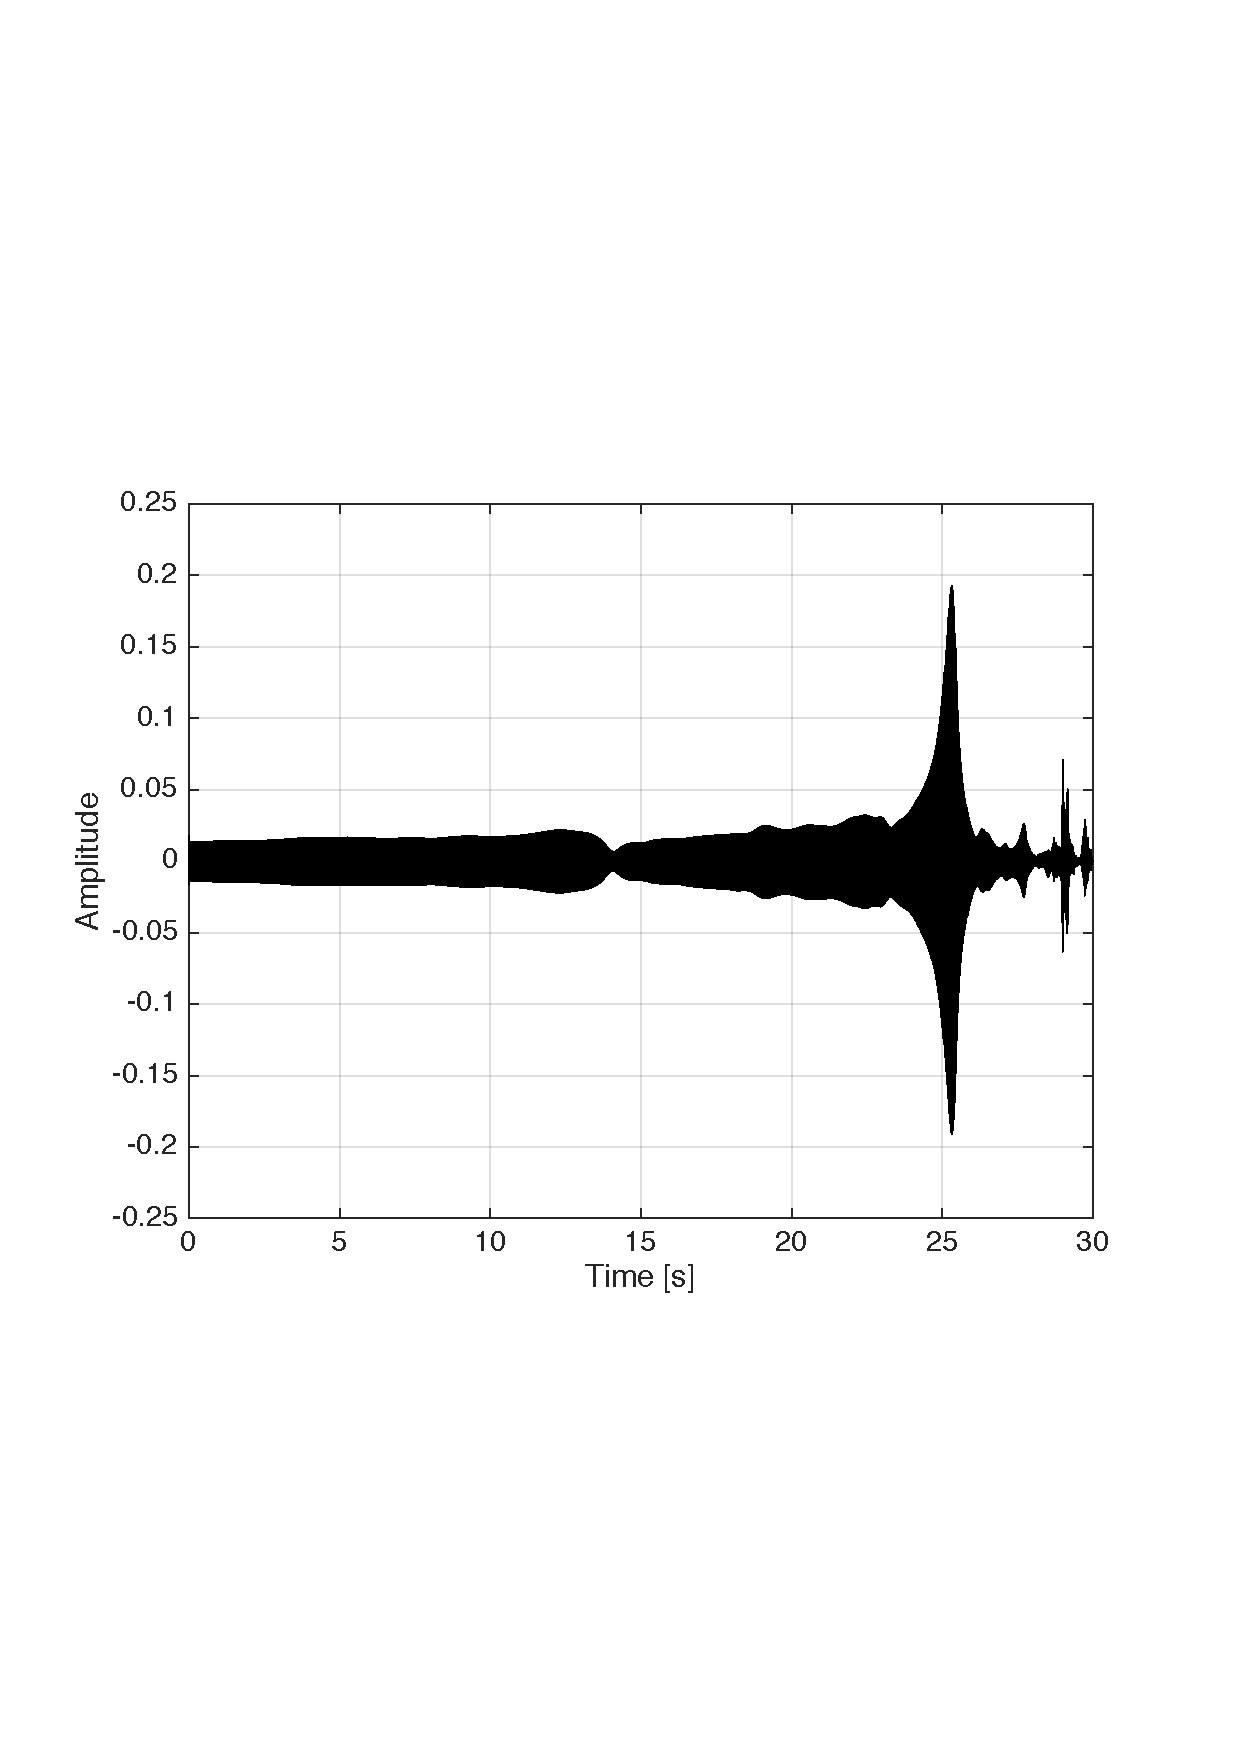
\includegraphics[width=\textwidth]{raw_driver19}
%% This file was created by matlab2tikz.
%
%The latest updates can be retrieved from
%  http://www.mathworks.com/matlabcentral/fileexchange/22022-matlab2tikz-matlab2tikz
%where you can also make suggestions and rate matlab2tikz.
%
\begin{tikzpicture}

\begin{axis}[%
width=1.6in,
height=1.2in,
at={(0.758in,0.481in)},
scale only axis,
xmin=0,
xmax=30,
xmajorgrids,
ymin=-0.2,
ymax=0.2,
ymajorgrids,
xlabel={Time [s]},
ylabel={Amplitude [V]},
axis background/.style={fill=white}
]
\addplot[fill=black,draw=black,forget plot] plot table[row sep=crcr]{%
2.08333333333333e-05	0.0174441337585449\\
0.0417454218822439	0.0131838321685791\\
0.0834700104311544	0.0131036043167114\\
0.125194598980065	0.0131006240844727\\
0.166919187528975	0.0131523609161377\\
0.208643776077886	0.0131937265396118\\
0.250368364626797	0.013242244720459\\
0.292092953175707	0.0132843255996704\\
0.333817541724618	0.0133000612258911\\
0.375542130273528	0.0133227109909058\\
0.417266718822439	0.0133814811706543\\
0.458991307371349	0.0134208202362061\\
0.50071589592026	0.0134570598602295\\
0.54244048446917	0.0134916305541992\\
0.584165073018081	0.0135313272476196\\
0.625889661566991	0.0135787725448608\\
0.667614250115902	0.0136535167694092\\
0.709338838664812	0.0136919021606445\\
0.751063427213723	0.0137407779693604\\
0.792788015762633	0.01378333568573\\
0.834512604311544	0.0138405561447144\\
0.876237192860454	0.0138554573059082\\
0.917961781409365	0.0138992071151733\\
0.959686369958275	0.0139317512512207\\
1.00141095850719	0.0139665603637695\\
1.0431355470561	0.0140010118484497\\
1.08486013560501	0.0140565633773804\\
1.12658472415392	0.0140770673751831\\
1.16830931270283	0.0141662359237671\\
1.21003390125174	0.0141417980194092\\
1.25175848980065	0.014143705368042\\
1.29348307834956	0.0142022371292114\\
1.33520766689847	0.014235258102417\\
1.37693225544738	0.0142310857772827\\
1.41865684399629	0.0142514705657959\\
1.4603814325452	0.0142501592636108\\
1.50210602109411	0.0142426490783691\\
1.54383060964302	0.0142196416854858\\
1.58555519819193	0.0141897201538086\\
1.62727978674084	0.0141717195510864\\
1.66900437528975	0.0141562223434448\\
1.71072896383866	0.0141338109970093\\
1.75245355238758	0.0141158103942871\\
1.79417814093649	0.0141069889068604\\
1.8359027294854	0.014079213142395\\
1.87762731803431	0.0140920877456665\\
1.91935190658322	0.0140824317932129\\
1.96107649513213	0.014080286026001\\
2.00280108368104	0.0140819549560547\\
2.04452567222995	0.0140804052352905\\
2.08625026077886	0.0140907764434814\\
2.12797484932777	0.0141453742980957\\
2.16969943787668	0.0141212940216064\\
2.21142402642559	0.014117956161499\\
2.2531486149745	0.0141592025756836\\
2.29487320352341	0.0141942501068115\\
2.33659779207232	0.0142147541046143\\
2.37832238062123	0.014255166053772\\
2.42004696917014	0.0142718553543091\\
2.46177155771905	0.0143097639083862\\
2.50349614626796	0.0143415927886963\\
2.54522073481687	0.0143803358078003\\
2.58694532336579	0.0144282579421997\\
2.6286699119147	0.014466404914856\\
2.67039450046361	0.0145164728164673\\
2.71211908901252	0.0145268440246582\\
2.75384367756143	0.0145998001098633\\
2.79556826611034	0.014657735824585\\
2.83729285465925	0.0147078037261963\\
2.87901744320816	0.014757513999939\\
2.92074203175707	0.0148080587387085\\
2.96246662030598	0.0148706436157227\\
3.00419120885489	0.0149272680282593\\
3.0459157974038	0.0149846076965332\\
3.08764038595271	0.0150657892227173\\
3.12936497450162	0.0151398181915283\\
3.17108956305053	0.0152368545532227\\
3.21281415159944	0.0153077840805054\\
3.25453874014835	0.0153566598892212\\
3.29626332869726	0.0154335498809814\\
3.33798791724618	0.0155411958694458\\
3.37971250579509	0.0155764818191528\\
3.421437094344	0.0156253576278687\\
3.46316168289291	0.0156955718994141\\
3.50488627144182	0.015771746635437\\
3.54661085999073	0.0158456563949585\\
3.58833544853964	0.0159142017364502\\
3.63006003708855	0.0159842967987061\\
3.67178462563746	0.0160502195358276\\
3.71350921418637	0.0160926580429077\\
3.75523380273528	0.0161477327346802\\
3.79695839128419	0.01618492603302\\
3.8386829798331	0.0162196159362793\\
3.88040756838201	0.0162382125854492\\
3.92213215693092	0.0162550210952759\\
3.96385674547983	0.0162825584411621\\
4.00558133402874	0.0162662267684937\\
4.04730592257765	0.0162646770477295\\
4.08903051112656	0.0162562131881714\\
4.13075509967547	0.0162286758422852\\
4.17247968822439	0.0162371397018433\\
4.2142042767733	0.0162320137023926\\
4.25592886532221	0.0162011384963989\\
4.29765345387112	0.0161941051483154\\
4.33937804242003	0.0161887407302856\\
4.38110263096894	0.0161789655685425\\
4.42282721951785	0.0162254571914673\\
4.46455180806676	0.0162070989608765\\
4.50627639661567	0.0162445306777954\\
4.54800098516458	0.0162758827209473\\
4.58972557371349	0.0163146257400513\\
4.6314501622624	0.0163501501083374\\
4.67317475081131	0.0163940191268921\\
4.71489933936022	0.0164343118667603\\
4.75662392790913	0.0164703130722046\\
4.79834851645804	0.0165045261383057\\
4.84007310500695	0.0165075063705444\\
4.88179769355586	0.0165128707885742\\
4.92352228210478	0.0165145397186279\\
4.96524687065368	0.0165392160415649\\
5.0069714592026	0.0165344476699829\\
5.04869604775151	0.0165383815765381\\
5.09042063630042	0.0165327787399292\\
5.13214522484933	0.0165436267852783\\
5.17386981339824	0.0165482759475708\\
5.21559440194715	0.0165524482727051\\
5.25731899049606	0.0165770053863525\\
5.29904357904497	0.0165486335754395\\
5.34076816759388	0.016539454460144\\
5.38249275614279	0.0165292024612427\\
5.4242173446917	0.0165091753005981\\
5.46594193324061	0.01650071144104\\
5.50766652178952	0.0164941549301147\\
5.54939111033843	0.0164557695388794\\
5.59111569888734	0.0164422988891602\\
5.63284028743625	0.0164107084274292\\
5.67456487598516	0.0163847208023071\\
5.71628946453407	0.0163488388061523\\
5.75801405308299	0.0162984132766724\\
5.7997386416319	0.016254186630249\\
5.84146323018081	0.0161999464035034\\
5.88318781872972	0.0161627531051636\\
5.92491240727863	0.016115665435791\\
5.96663699582754	0.0160861015319824\\
6.00836158437645	0.0160255432128906\\
6.05008617292536	0.0159963369369507\\
6.09181076147427	0.0159608125686646\\
6.13353535002318	0.015892505645752\\
6.17525993857209	0.0158644914627075\\
6.216984527121	0.0158439874649048\\
6.25870911566991	0.0158376693725586\\
6.30043370421882	0.015795111656189\\
6.34215829276773	0.0157642364501953\\
6.38388288131664	0.0157539844512939\\
6.42560746986555	0.0157680511474609\\
6.46733205841446	0.0157626867294312\\
6.50905664696338	0.0157822370529175\\
6.55078123551229	0.0157889127731323\\
6.5925058240612	0.01578688621521\\
6.63423041261011	0.015788197517395\\
6.67595500115902	0.0158027410507202\\
6.71767958970793	0.0158090591430664\\
6.75940417825684	0.0158181190490723\\
6.80112876680575	0.0158118009567261\\
6.84285335535466	0.0158218145370483\\
6.88457794390357	0.0158369541168213\\
6.92630253245248	0.0158761739730835\\
6.96802712100139	0.0158882141113281\\
7.0097517095503	0.0159152746200562\\
7.05147629809921	0.015964150428772\\
7.09320088664812	0.0159767866134644\\
7.13492547519703	0.0160250663757324\\
7.17665006374594	0.0161073207855225\\
7.21837465229485	0.0161528587341309\\
7.26009924084376	0.0162261724472046\\
7.30182382939268	0.0163071155548096\\
7.34354841794159	0.0163383483886719\\
7.3852730064905	0.016379714012146\\
7.42699759503941	0.0164109468460083\\
7.46872218358832	0.0164202451705933\\
7.51044677213723	0.01641845703125\\
7.55217136068614	0.0163893699645996\\
7.59389594923505	0.0163551568984985\\
7.63562053778396	0.016291618347168\\
7.67734512633287	0.0162198543548584\\
7.71906971488178	0.0161285400390625\\
7.76079430343069	0.016048789024353\\
7.8025188919796	0.0159471035003662\\
7.84424348052851	0.0158181190490723\\
7.88596806907742	0.0157514810562134\\
7.92769265762633	0.0156846046447754\\
7.96941724617524	0.0156430006027222\\
8.01114183472416	0.0156441926956177\\
8.05286642327307	0.015630841255188\\
8.09459101182198	0.0156680345535278\\
8.13631560037089	0.015711784362793\\
8.1780401889198	0.0157798528671265\\
8.21976477746871	0.0158299207687378\\
8.26148936601762	0.0159074068069458\\
8.30321395456653	0.0159891843795776\\
8.34493854311544	0.01605224609375\\
8.38666313166435	0.0161564350128174\\
8.42838772021326	0.0162137746810913\\
8.47011230876217	0.0163058042526245\\
8.51183689731108	0.0163658857345581\\
8.55356148585999	0.0164523124694824\\
8.5952860744089	0.0164806842803955\\
8.63701066295781	0.0166155099868774\\
8.67873525150672	0.0166575908660889\\
8.72045984005563	0.0167548656463623\\
8.76218442860454	0.016825795173645\\
8.80390901715345	0.0169020891189575\\
8.84563360570237	0.0169821977615356\\
8.88735819425128	0.0170701742172241\\
8.92908278280018	0.0171375274658203\\
8.9708073713491	0.0171587467193604\\
9.01253195989801	0.017237663269043\\
9.05425654844692	0.0172935724258423\\
9.09598113699583	0.0173218250274658\\
9.13770572554474	0.0173497200012207\\
9.17943031409365	0.0173822641372681\\
9.22115490264256	0.0174020528793335\\
9.26287949119147	0.0174028873443604\\
9.30460407974038	0.0174020528793335\\
9.34632866828929	0.017397403717041\\
9.3880532568382	0.017382025718689\\
9.42977784538711	0.0173323154449463\\
9.47150243393602	0.0173298120498657\\
9.51322702248493	0.0173071622848511\\
9.55495161103384	0.0172981023788452\\
9.59667619958275	0.0172533988952637\\
9.63840078813166	0.0172268152236938\\
9.68012537668058	0.0172126293182373\\
9.72184996522949	0.0172011852264404\\
9.7635745537784	0.0171804428100586\\
9.80529914232731	0.0171520709991455\\
9.84702373087622	0.0171386003494263\\
9.88874831942513	0.0171166658401489\\
9.93047290797404	0.0170993804931641\\
9.97219749652295	0.0170501470565796\\
10.0139220850719	0.0170356035232544\\
10.0556466736208	0.0170102119445801\\
10.0973712621697	0.0169705152511597\\
10.1390958507186	0.0169491767883301\\
10.1808204392675	0.0169264078140259\\
10.2225450278164	0.0169349908828735\\
10.2642696163653	0.016948938369751\\
10.3059942049142	0.0169826745986938\\
10.3477187934631	0.0170327425003052\\
10.3894433820121	0.0170915126800537\\
10.431167970561	0.0171574354171753\\
10.4728925591099	0.0172317028045654\\
10.5146171476588	0.0172722339630127\\
10.5563417362077	0.0173627138137817\\
10.5980663247566	0.0174278020858765\\
10.6397909133055	0.0175130367279053\\
10.6815155018544	0.0175483226776123\\
10.7232400904033	0.0176342725753784\\
10.7649646789523	0.0176903009414673\\
10.8066892675012	0.0177403688430786\\
10.8484138560501	0.0177834033966064\\
10.890138444599	0.0178585052490234\\
10.9318630331479	0.0179126262664795\\
10.9735876216968	0.0179930925369263\\
11.0153122102457	0.0180377960205078\\
11.0570367987946	0.0181233882904053\\
11.0987613873435	0.0181983709335327\\
11.1404859758924	0.0183128118515015\\
11.1822105644414	0.0184154510498047\\
11.2239351529903	0.0185511112213135\\
11.2656597415392	0.0186648368835449\\
11.3073843300881	0.0188018083572388\\
11.349108918637	0.0189625024795532\\
11.3908335071859	0.0190943479537964\\
11.4325580957348	0.0192328691482544\\
11.4742826842837	0.0194246768951416\\
11.5160072728326	0.0195508003234863\\
11.5577318613816	0.019692063331604\\
11.5994564499305	0.0198198556900024\\
11.6411810384794	0.0199755430221558\\
11.6829056270283	0.0201060771942139\\
11.7246302155772	0.0202442407608032\\
11.7663548041261	0.0203926563262939\\
11.808079392675	0.0205307006835938\\
11.8498039812239	0.0206559896469116\\
11.8915285697728	0.0208258628845215\\
11.9332531583217	0.0209463834762573\\
11.9749777468707	0.0210902690887451\\
12.0167023354196	0.0212063789367676\\
12.0584269239685	0.0213172435760498\\
12.1001515125174	0.0214052200317383\\
12.1418761010663	0.0215300321578979\\
12.1836006896152	0.0216346979141235\\
12.2253252781641	0.0217214822769165\\
12.267049866713	0.0217512845993042\\
12.3087744552619	0.0217386484146118\\
12.3504990438108	0.0217629671096802\\
12.3922236323598	0.0217190980911255\\
12.4339482209087	0.0217164754867554\\
12.4756728094576	0.0216211080551147\\
12.5173973980065	0.0215216875076294\\
12.5591219865554	0.0214111804962158\\
12.6008465751043	0.0212830305099487\\
12.6425711636532	0.0211762189865112\\
12.6842957522021	0.0210355520248413\\
12.726020340751	0.0209170579910278\\
12.7677449293	0.0208185911178589\\
12.8094695178489	0.0207177400588989\\
12.8511941063978	0.0206308364868164\\
12.8929186949467	0.0205261707305908\\
12.9346432834956	0.0204188823699951\\
12.9763678720445	0.0203160047531128\\
13.0180924605934	0.0202019214630127\\
13.0598170491423	0.020089864730835\\
13.1015416376912	0.0199722051620483\\
13.1432662262401	0.0198445320129395\\
13.1849908147891	0.0197038650512695\\
13.226715403338	0.0195189714431763\\
13.2684399918869	0.0193073749542236\\
13.3101645804358	0.0190596580505371\\
13.3518891689847	0.0188181400299072\\
13.3936137575336	0.0185122489929199\\
13.4353383460825	0.0181918144226074\\
13.4770629346314	0.0177853107452393\\
13.5187875231803	0.0173110961914063\\
13.5605121117293	0.0167787075042725\\
13.6022367002782	0.0161740779876709\\
13.6439612888271	0.0155293941497803\\
13.685685877376	0.0147796869277954\\
13.7274104659249	0.0139639377593994\\
13.7691350544738	0.0130655765533447\\
13.8108596430227	0.0121190547943115\\
13.8525842315716	0.011111855506897\\
13.8943088201205	0.0100915431976318\\
13.9360334086694	0.00906765460968018\\
13.9777579972184	0.0081101655960083\\
14.0194825857673	0.00735759735107422\\
14.0612071743162	0.00674760341644287\\
14.1029317628651	0.00652647018432617\\
14.144656351414	0.00688815116882324\\
14.1863809399629	0.00745463371276855\\
14.2281055285118	0.00815272331237793\\
14.2698301170607	0.00885546207427979\\
14.3115547056096	0.00954830646514893\\
14.3532792941586	0.0101321935653687\\
14.3950038827075	0.0106920003890991\\
14.4367284712564	0.0111517906188965\\
14.4784530598053	0.0115351676940918\\
14.5201776483542	0.0118722915649414\\
14.5619022369031	0.0121043920516968\\
14.603626825452	0.0123043060302734\\
14.6453514140009	0.0124328136444092\\
14.6870760025498	0.0125536918640137\\
14.7288005910988	0.0126279592514038\\
14.7705251796477	0.0126522779464722\\
14.8122497681966	0.0126771926879883\\
14.8539743567455	0.0126643180847168\\
14.8956989452944	0.0126442909240723\\
14.9374235338433	0.0126314163208008\\
14.9791481223922	0.0126005411148071\\
15.0208727109411	0.0125870704650879\\
15.06259729949	0.0126197338104248\\
15.1043218880389	0.0127360820770264\\
15.1460464765879	0.0129470825195313\\
15.1877710651368	0.0131411552429199\\
15.2294956536857	0.0134528875350952\\
15.2712202422346	0.0137631893157959\\
15.3129448307835	0.014081597328186\\
15.3546694193324	0.0143324136734009\\
15.3963940078813	0.0145440101623535\\
15.4381185964302	0.0147069692611694\\
15.4798431849791	0.014826774597168\\
15.521567773528	0.0149147510528564\\
15.563292362077	0.0150187015533447\\
15.6050169506259	0.0150867700576782\\
15.6467415391748	0.0151418447494507\\
15.6884661277237	0.0152006149291992\\
15.7301907162726	0.0152875185012817\\
15.7719153048215	0.015317440032959\\
15.8136398933704	0.0153570175170898\\
15.8553644819193	0.0153845548629761\\
15.8970890704682	0.0154201984405518\\
15.9388136590172	0.0154287815093994\\
15.9805382475661	0.0154200792312622\\
16.022262836115	0.0154227018356323\\
16.0639874246639	0.0153900384902954\\
16.1057120132128	0.0153504610061646\\
16.1474366017617	0.0152820348739624\\
16.1891611903106	0.0152740478515625\\
16.2308857788595	0.0152736902236938\\
16.2726103674084	0.0152853727340698\\
16.3143349559573	0.0153579711914063\\
16.3560595445063	0.0154263973236084\\
16.3977841330552	0.0155422687530518\\
16.4395087216041	0.0156645774841309\\
16.481233310153	0.015790581703186\\
16.5229578987019	0.0159449577331543\\
16.5646824872508	0.0161056518554688\\
16.6064070757997	0.0162507295608521\\
16.6481316643486	0.0163685083389282\\
16.6898562528975	0.0164653062820435\\
16.7315808414465	0.0165603160858154\\
16.7733054299954	0.0167076587677002\\
16.8150300185443	0.0167895555496216\\
16.8567546070932	0.0168788433074951\\
16.8984791956421	0.0169848203659058\\
16.940203784191	0.017051100730896\\
16.9819283727399	0.017139196395874\\
17.0236529612888	0.0172312259674072\\
17.0653775498377	0.0173563957214355\\
17.1071021383867	0.0174448490142822\\
17.1488267269356	0.0174803733825684\\
17.1905513154845	0.0175639390945435\\
17.2322759040334	0.0176322460174561\\
17.2740004925823	0.0177028179168701\\
17.3157250811312	0.017791748046875\\
17.3574496696801	0.0178496837615967\\
17.399174258229	0.0178979635238647\\
17.4408988467779	0.017961859703064\\
17.4826234353268	0.018022894859314\\
17.5243480238758	0.018062949180603\\
17.5660726124247	0.01810622215271\\
17.6077972009736	0.0180763006210327\\
17.6495217895225	0.0180815458297729\\
17.6912463780714	0.0180732011795044\\
17.7329709666203	0.0180991888046265\\
17.7746955551692	0.0181357860565186\\
17.8164201437181	0.018202543258667\\
17.858144732267	0.0183231830596924\\
17.8998693208159	0.0184512138366699\\
17.9415939093649	0.0185703039169312\\
17.9833184979138	0.0187492370605469\\
18.0250430864627	0.0189353227615356\\
18.0667676750116	0.0190675258636475\\
18.1084922635605	0.0192264318466187\\
18.1502168521094	0.0192973613739014\\
18.1919414406583	0.0193362236022949\\
18.2336660292072	0.0193533897399902\\
18.2753906177561	0.0193248987197876\\
18.3171152063051	0.0193346738815308\\
18.358839794854	0.0192720890045166\\
18.4005643834029	0.0192611217498779\\
18.4422889719518	0.0192636251449585\\
18.4840135605007	0.0192739963531494\\
18.5257381490496	0.0192903280258179\\
18.5674627375985	0.0194275379180908\\
18.6091873261474	0.0196996927261353\\
18.6509119146963	0.0200306177139282\\
18.6926365032453	0.0204979181289673\\
18.7343610917942	0.02104651927948\\
18.7760856803431	0.0216186046600342\\
18.817810268892	0.0222443342208862\\
18.8595348574409	0.0227910280227661\\
18.9012594459898	0.0233092308044434\\
18.9429840345387	0.023730993270874\\
18.9847086230876	0.0240856409072876\\
19.0264332116365	0.0244448184967041\\
19.0681578001854	0.0246785879135132\\
19.1098823887344	0.0248157978057861\\
19.1516069772833	0.0248291492462158\\
19.1933315658322	0.0247887372970581\\
19.2350561543811	0.0246955156326294\\
19.27678074293	0.0245308876037598\\
19.3185053314789	0.0243546962738037\\
19.3602299200278	0.0240871906280518\\
19.4019545085767	0.0237839221954346\\
19.4436790971256	0.0234526395797729\\
19.4854036856745	0.0231184959411621\\
19.5271282742235	0.022815465927124\\
19.5688528627724	0.0225284099578857\\
19.6105774513213	0.0223060846328735\\
19.6523020398702	0.0221070051193237\\
19.6940266284191	0.0219635963439941\\
19.735751216968	0.0218530893325806\\
19.7774758055169	0.0217581987380981\\
19.8192003940658	0.0217596292495728\\
19.8609249826147	0.0217828750610352\\
19.9026495711637	0.0218667984008789\\
19.9443741597126	0.0219509601593018\\
19.9860987482615	0.0220874547958374\\
20.0278233368104	0.0222543478012085\\
20.0695479253593	0.0224721431732178\\
20.1112725139082	0.0226690769195557\\
20.1529971024571	0.0229157209396362\\
20.194721691006	0.0231697559356689\\
20.2364462795549	0.0234352350234985\\
20.2781708681038	0.0237188339233398\\
20.3198954566528	0.0240160226821899\\
20.3616200452017	0.0242964029312134\\
20.4033446337506	0.024566650390625\\
20.4450692222995	0.0247782468795776\\
20.4867938108484	0.0249801874160767\\
20.5285183993973	0.025060772895813\\
20.5702429879462	0.0250948667526245\\
20.6119675764951	0.0251015424728394\\
20.653692165044	0.025084376335144\\
20.695416753593	0.0250260829925537\\
20.7371413421419	0.0249568223953247\\
20.7788659306908	0.0249083042144775\\
20.8205905192397	0.0248545408248901\\
20.8623151077886	0.0248538255691528\\
20.9040396963375	0.0248321294784546\\
20.9457642848864	0.0248123407363892\\
20.9874888734353	0.0247715711593628\\
21.0292134619842	0.0246872901916504\\
21.0709380505331	0.0245916843414307\\
21.1126626390821	0.0244895219802856\\
21.154387227631	0.0243560075759888\\
21.1961118161799	0.0242257118225098\\
21.2378364047288	0.0241231918334961\\
21.2795609932777	0.0240743160247803\\
21.3212855818266	0.0240955352783203\\
21.3630101703755	0.0242211818695068\\
21.4047347589244	0.0243576765060425\\
21.4464593474733	0.0245411396026611\\
21.4881839360223	0.0248323678970337\\
21.5299085245712	0.0251299142837524\\
21.5716331131201	0.0254895687103271\\
21.613357701669	0.0259164571762085\\
21.6550822902179	0.0263410806655884\\
21.6968068787668	0.0268235206604004\\
21.7385314673157	0.0273033380508423\\
21.7802560558646	0.0278036594390869\\
21.8219806444135	0.0282833576202393\\
21.8637052329624	0.0288461446762085\\
21.9054298215114	0.0293409824371338\\
21.9471544100603	0.0298067331314087\\
21.9888789986092	0.0302213430404663\\
22.0306035871581	0.0305540561676025\\
22.072328175707	0.0307530164718628\\
22.1140527642559	0.0307987928390503\\
22.1557773528048	0.030825138092041\\
22.1975019413537	0.0308418273925781\\
22.2392265299026	0.0311071872711182\\
22.2809511184516	0.0313805341720581\\
22.3226757070005	0.0317173004150391\\
22.3644002955494	0.0320000648498535\\
22.4061248840983	0.0321570634841919\\
22.4478494726472	0.0321915149688721\\
22.4895740611961	0.0321606397628784\\
22.531298649745	0.031922459602356\\
22.5730232382939	0.0316141843795776\\
22.6147478268428	0.0312548875808716\\
22.6564724153917	0.0308171510696411\\
22.6981970039407	0.0305826663970947\\
22.7399215924896	0.0304679870605469\\
22.7816461810385	0.0303603410720825\\
22.8233707695874	0.0304563045501709\\
22.8650953581363	0.0305367708206177\\
22.9068199466852	0.0306057929992676\\
22.9485445352341	0.0306912660598755\\
22.990269123783	0.0306066274642944\\
23.0319937123319	0.0304591655731201\\
23.0737183008809	0.0297863483428955\\
23.1154428894298	0.0285071134567261\\
23.1571674779787	0.027154803276062\\
23.1988920665276	0.0259910821914673\\
23.2406166550765	0.0244603157043457\\
23.2823412436254	0.0236220359802246\\
23.3240658321743	0.0235285758972168\\
23.3657904207232	0.0241098403930664\\
23.4075150092721	0.0248513221740723\\
23.449239597821	0.0258579254150391\\
23.49096418637	0.0267441272735596\\
23.5326887749189	0.0276174545288086\\
23.5744133634678	0.0282967090606689\\
23.6161379520167	0.0288980007171631\\
23.6578625405656	0.0294115543365479\\
23.6995871291145	0.0299835205078125\\
23.7413117176634	0.0305644273757935\\
23.7830363062123	0.0313618183135986\\
23.8247608947612	0.0322580337524414\\
23.8664854833102	0.0332018136978149\\
23.9082100718591	0.0342499017715454\\
23.949934660408	0.035599946975708\\
23.9916592489569	0.0370364189147949\\
24.0333838375058	0.0383732318878174\\
24.0751084260547	0.0398944616317749\\
24.1168330146036	0.041479229927063\\
24.1585576031525	0.0429228544235229\\
24.2002821917014	0.0444319248199463\\
24.2420067802503	0.0459293127059937\\
24.2837313687993	0.047610878944397\\
24.3254559573482	0.0492688417434692\\
24.3671805458971	0.0510417222976685\\
24.408905134446	0.0529109239578247\\
24.4506297229949	0.0548422336578369\\
24.4923543115438	0.056898832321167\\
24.5340789000927	0.0591094493865967\\
24.5758034886416	0.0617804527282715\\
24.6175280771905	0.0645843744277954\\
24.6592526657395	0.0677156448364258\\
24.7009772542884	0.0712670087814331\\
24.7427018428373	0.0752949714660645\\
24.7844264313862	0.0799596309661865\\
24.8261510199351	0.0852384567260742\\
24.867875608484	0.0909876823425293\\
24.9096001970329	0.0979855060577393\\
24.9513247855818	0.105462312698364\\
24.9930493741307	0.114107251167297\\
25.0347739626796	0.123892664909363\\
25.0764985512286	0.1347895860672\\
25.1182231397775	0.146229147911072\\
25.1599477283264	0.158706545829773\\
25.2016723168753	0.170397281646729\\
25.2433969054242	0.181927919387817\\
25.2851214939731	0.190452098846436\\
25.326846082522	0.192880272865295\\
25.3685706710709	0.192157387733459\\
25.4102952596198	0.181955933570862\\
25.4520198481687	0.162297606468201\\
25.4937444367177	0.13434636592865\\
25.5354690252666	0.109553933143616\\
25.5771936138155	0.0896941423416138\\
25.6189182023644	0.0760148763656616\\
25.6606427909133	0.0651895999908447\\
25.7023673794622	0.0563890933990479\\
25.7440919680111	0.0492444038391113\\
25.78581655656	0.043710470199585\\
25.8275411451089	0.0384472608566284\\
25.8692657336579	0.0339940786361694\\
25.9109903222068	0.0300600528717041\\
25.9527149107557	0.0264880657196045\\
25.9944394993046	0.0233311653137207\\
26.0361640878535	0.0206685066223145\\
26.0778886764024	0.0186737775802612\\
26.1196132649513	0.0171686410903931\\
26.1613378535002	0.0166844129562378\\
26.2030624420491	0.017844557762146\\
26.2447870305981	0.0197421312332153\\
26.286511619147	0.0215028524398804\\
26.3282362076959	0.0223579406738281\\
26.3699607962448	0.0223031044006348\\
26.4116853847937	0.0217078924179077\\
26.4534099733426	0.0204193592071533\\
26.4951345618915	0.0195810794830322\\
26.5368591504404	0.0191034078598022\\
26.5785837389893	0.0182909965515137\\
26.6203083275383	0.01659095287323\\
26.6620329160872	0.0147438049316406\\
26.7037575046361	0.0134490728378296\\
26.745482093185	0.012037992477417\\
26.7872066817339	0.0107738971710205\\
26.8289312702828	0.00990462303161621\\
26.8706558588317	0.00957143306732178\\
26.9123804473806	0.00931215286254883\\
26.9541050359295	0.0092695951461792\\
26.9958296244784	0.0102084875106812\\
27.0375542130274	0.0113158226013184\\
27.0792788015763	0.0121122598648071\\
27.1210033901252	0.0121549367904663\\
27.1627279786741	0.0111083984375\\
27.204452567223	0.00957083702087402\\
27.2461771557719	0.00859379768371582\\
27.2879017443208	0.00834882259368896\\
27.3296263328697	0.00859546661376953\\
27.3713509214186	0.0090184211730957\\
27.4130755099675	0.00977170467376709\\
27.4548000985165	0.0107346773147583\\
27.4965246870654	0.012182354927063\\
27.5382492756143	0.0141066312789917\\
27.5799738641632	0.0166143178939819\\
27.6216984527121	0.0203871726989746\\
27.663423041261	0.0240563154220581\\
27.7051476298099	0.0260938405990601\\
27.7468722183588	0.0261249542236328\\
27.7885968069077	0.0226942300796509\\
27.8303213954567	0.0153995752334595\\
27.8720459840056	0.0115272998809814\\
27.9137705725545	0.00934135913848877\\
27.9554951611034	0.00725364685058594\\
27.9972197496523	0.00573289394378662\\
28.0389443382012	0.00476109981536865\\
28.0806689267501	0.00405430793762207\\
28.122393515299	0.00347089767456055\\
28.1641181038479	0.00348937511444092\\
28.2058426923968	0.0043492317199707\\
28.2475672809458	0.00484251976013184\\
28.2892918694947	0.00487172603607178\\
28.3310164580436	0.00547254085540771\\
28.3727410465925	0.00589895248413086\\
28.4144656351414	0.00629270076751709\\
28.4561902236903	0.00670242309570313\\
28.4979148122392	0.00694727897644043\\
28.5396394007881	0.00746893882751465\\
28.581363989337	0.00698328018188477\\
28.623088577886	0.00598013401031494\\
28.6648131664349	0.0123151540756226\\
28.7065377549838	0.0124528408050537\\
28.7482623435327	0.0158895254135132\\
28.7899869320816	0.0123809576034546\\
28.8317115206305	0.00990724563598633\\
28.8734361091794	0.0101600885391235\\
28.9151606977283	0.00902903079986572\\
28.9568852862772	0.00959169864654541\\
28.9986098748261	0.0708549022674561\\
29.0403344633751	0.0490773916244507\\
29.082059051924	0.0367391109466553\\
29.1237836404729	0.0392665863037109\\
29.1655082290218	0.0501984357833862\\
29.2072328175707	0.0316517353057861\\
29.2489574061196	0.0146907567977905\\
29.2906819946685	0.0124069452285767\\
29.3324065832174	0.0109615325927734\\
29.3741311717663	0.00983536243438721\\
29.4158557603153	0.00371837615966797\\
29.4575803488642	0.00346684455871582\\
29.4993049374131	0.0025477409362793\\
29.541029525962	0.0020139217376709\\
29.5827541145109	0.00222396850585938\\
29.6244787030598	0.0047835111618042\\
29.6662032916087	0.0106549263000488\\
29.7079278801576	0.0227276086807251\\
29.7496524687065	0.0288950204849243\\
29.7913770572554	0.0240693092346191\\
29.8331016458044	0.0165066719055176\\
29.8748262343533	0.0114091634750366\\
29.9165508229022	0.00875699520111084\\
29.9582754114511	0.00749635696411133\\
30	0.00196146965026855\\
}
\closedcycle;
\addplot[fill=black,draw=black,forget plot] plot table[row sep=crcr]{%
2.08333333333333e-05	-0.0159932374954224\\
0.0417454218822439	-0.0136831998825073\\
0.0834700104311544	-0.0136864185333252\\
0.125194598980065	-0.0137081146240234\\
0.166919187528975	-0.0137027502059937\\
0.208643776077886	-0.0137177705764771\\
0.250368364626797	-0.0137653350830078\\
0.292092953175707	-0.0137816667556763\\
0.333817541724618	-0.0138300657272339\\
0.375542130273528	-0.0138695240020752\\
0.417266718822439	-0.0139075517654419\\
0.458991307371349	-0.0139497518539429\\
0.50071589592026	-0.0140053033828735\\
0.54244048446917	-0.0140515565872192\\
0.584165073018081	-0.0140962600708008\\
0.625889661566991	-0.0141353607177734\\
0.667614250115902	-0.0141550302505493\\
0.709338838664812	-0.0141642093658447\\
0.751063427213723	-0.0142364501953125\\
0.792788015762633	-0.0142496824264526\\
0.834512604311544	-0.0143007040023804\\
0.876237192860454	-0.0143524408340454\\
0.917961781409365	-0.0143682956695557\\
0.959686369958275	-0.0144027471542358\\
1.00141095850719	-0.0144290924072266\\
1.0431355470561	-0.0144684314727783\\
1.08486013560501	-0.0145009756088257\\
1.12658472415392	-0.0145292282104492\\
1.16830931270283	-0.0145310163497925\\
1.21003390125174	-0.0145913362503052\\
1.25175848980065	-0.0146056413650513\\
1.29348307834956	-0.014609694480896\\
1.33520766689847	-0.014613151550293\\
1.37693225544738	-0.0146564245223999\\
1.41865684399629	-0.0147069692611694\\
1.4603814325452	-0.0147548913955688\\
1.50210602109411	-0.0147720575332642\\
1.54383060964302	-0.0147882699966431\\
1.58555519819193	-0.0148137807846069\\
1.62727978674084	-0.0147954225540161\\
1.66900437528975	-0.0147997140884399\\
1.71072896383866	-0.014802098274231\\
1.75245355238758	-0.0147850513458252\\
1.79417814093649	-0.0147900581359863\\
1.8359027294854	-0.0147967338562012\\
1.87762731803431	-0.0147658586502075\\
1.91935190658322	-0.0147805213928223\\
1.96107649513213	-0.0147795677185059\\
2.00280108368104	-0.0147765874862671\\
2.04452567222995	-0.0148054361343384\\
2.08625026077886	-0.0148167610168457\\
2.12797484932777	-0.0148104429244995\\
2.16969943787668	-0.014845609664917\\
2.21142402642559	-0.0148526430130005\\
2.2531486149745	-0.0148493051528931\\
2.29487320352341	-0.0148800611495972\\
2.33659779207232	-0.0149073600769043\\
2.37832238062123	-0.0149215459823608\\
2.42004696917014	-0.0149686336517334\\
2.46177155771905	-0.0149891376495361\\
2.50349614626796	-0.0150300264358521\\
2.54522073481687	-0.015070915222168\\
2.58694532336579	-0.0150928497314453\\
2.6286699119147	-0.0151451826095581\\
2.67039450046361	-0.0151525735855103\\
2.71211908901252	-0.0152038335800171\\
2.75384367756143	-0.0152643918991089\\
2.79556826611034	-0.0153129100799561\\
2.83729285465925	-0.0153428316116333\\
2.87901744320816	-0.0154058933258057\\
2.92074203175707	-0.015446662902832\\
2.96246662030598	-0.0155152082443237\\
3.00419120885489	-0.0156008005142212\\
3.0459157974038	-0.015687108039856\\
3.08764038595271	-0.015765905380249\\
3.12936497450162	-0.0158531665802002\\
3.17108956305053	-0.0159111022949219\\
3.21281415159944	-0.0159949064254761\\
3.25453874014835	-0.0161058902740479\\
3.29626332869726	-0.0161623954772949\\
3.33798791724618	-0.0162557363510132\\
3.37971250579509	-0.0163384675979614\\
3.421437094344	-0.0164409875869751\\
3.46316168289291	-0.0165195465087891\\
3.50488627144182	-0.0165740251541138\\
3.54661085999073	-0.0166549682617188\\
3.58833544853964	-0.0167381763458252\\
3.63006003708855	-0.0167884826660156\\
3.67178462563746	-0.0168477296829224\\
3.71350921418637	-0.016872763633728\\
3.75523380273528	-0.0168941020965576\\
3.79695839128419	-0.0169187784194946\\
3.8386829798331	-0.0169479846954346\\
3.88040756838201	-0.0169333219528198\\
3.92213215693092	-0.016893744468689\\
3.96385674547983	-0.0169346332550049\\
4.00558133402874	-0.0168807506561279\\
4.04730592257765	-0.0168675184249878\\
4.08903051112656	-0.0168465375900269\\
4.13075509967547	-0.0168452262878418\\
4.17247968822439	-0.0168131589889526\\
4.2142042767733	-0.0167852640151978\\
4.25592886532221	-0.0167598724365234\\
4.29765345387112	-0.0167505741119385\\
4.33937804242003	-0.016740083694458\\
4.38110263096894	-0.0167372226715088\\
4.42282721951785	-0.0167292356491089\\
4.46455180806676	-0.0167250633239746\\
4.50627639661567	-0.0167497396469116\\
4.54800098516458	-0.0167809724807739\\
4.58972557371349	-0.0168344974517822\\
4.6314501622624	-0.0168977975845337\\
4.67317475081131	-0.0169267654418945\\
4.71489933936022	-0.0169526338577271\\
4.75662392790913	-0.0169451236724854\\
4.79834851645804	-0.0169491767883301\\
4.84007310500695	-0.0169534683227539\\
4.88179769355586	-0.0169605016708374\\
4.92352228210478	-0.0169579982757568\\
4.96524687065368	-0.0169459581375122\\
5.0069714592026	-0.0169612169265747\\
5.04869604775151	-0.0169461965560913\\
5.09042063630042	-0.016968846321106\\
5.13214522484933	-0.0169471502304077\\
5.17386981339824	-0.0169591903686523\\
5.21559440194715	-0.016942024230957\\
5.25731899049606	-0.0169354677200317\\
5.29904357904497	-0.0169334411621094\\
5.34076816759388	-0.016936182975769\\
5.38249275614279	-0.0169117450714111\\
5.4242173446917	-0.0169116258621216\\
5.46594193324061	-0.0169053077697754\\
5.50766652178952	-0.01686692237854\\
5.54939111033843	-0.0168808698654175\\
5.59111569888734	-0.0168665647506714\\
5.63284028743625	-0.0168148279190063\\
5.67456487598516	-0.0167924165725708\\
5.71628946453407	-0.0167427062988281\\
5.75801405308299	-0.0167151689529419\\
5.7997386416319	-0.0166959762573242\\
5.84146323018081	-0.0166800022125244\\
5.88318781872972	-0.0166391134262085\\
5.92491240727863	-0.0166083574295044\\
5.96663699582754	-0.0165565013885498\\
6.00836158437645	-0.016548752784729\\
6.05008617292536	-0.0165069103240967\\
6.09181076147427	-0.0164694786071777\\
6.13353535002318	-0.016451358795166\\
6.17525993857209	-0.0164226293563843\\
6.216984527121	-0.0163737535476685\\
6.25870911566991	-0.0163513422012329\\
6.30043370421882	-0.0163525342941284\\
6.34215829276773	-0.0163525342941284\\
6.38388288131664	-0.0163518190383911\\
6.42560746986555	-0.0163501501083374\\
6.46733205841446	-0.0163429975509644\\
6.50905664696338	-0.0163670778274536\\
6.55078123551229	-0.0163668394088745\\
6.5925058240612	-0.0163979530334473\\
6.63423041261011	-0.0164004564285278\\
6.67595500115902	-0.0164167881011963\\
6.71767958970793	-0.01643967628479\\
6.75940417825684	-0.0164421796798706\\
6.80112876680575	-0.0164488554000854\\
6.84285335535466	-0.016448974609375\\
6.88457794390357	-0.016472339630127\\
6.92630253245248	-0.0165094137191772\\
6.96802712100139	-0.0165352821350098\\
7.0097517095503	-0.0165783166885376\\
7.05147629809921	-0.0166103839874268\\
7.09320088664812	-0.0166771411895752\\
7.13492547519703	-0.0167235136032104\\
7.17665006374594	-0.016762375831604\\
7.21837465229485	-0.0168224573135376\\
7.26009924084376	-0.0168670415878296\\
7.30182382939268	-0.0168749094009399\\
7.34354841794159	-0.0169117450714111\\
7.3852730064905	-0.0169516801834106\\
7.42699759503941	-0.0169820785522461\\
7.46872218358832	-0.0169767141342163\\
7.51044677213723	-0.0169795751571655\\
7.55217136068614	-0.0169461965560913\\
7.59389594923505	-0.0169112682342529\\
7.63562053778396	-0.016893744468689\\
7.67734512633287	-0.0167742967605591\\
7.71906971488178	-0.016714334487915\\
7.76079430343069	-0.0166012048721313\\
7.8025188919796	-0.0164294242858887\\
7.84424348052851	-0.0163884162902832\\
7.88596806907742	-0.0163111686706543\\
7.92769265762633	-0.0162628889083862\\
7.96941724617524	-0.0162183046340942\\
8.01114183472416	-0.0162019729614258\\
8.05286642327307	-0.0162206888198853\\
8.09459101182198	-0.0162594318389893\\
8.13631560037089	-0.0162904262542725\\
8.1780401889198	-0.0163576602935791\\
8.21976477746871	-0.0164244174957275\\
8.26148936601762	-0.0165115594863892\\
8.30321395456653	-0.0165975093841553\\
8.34493854311544	-0.0166696310043335\\
8.38666313166435	-0.0167193412780762\\
8.42838772021326	-0.0168086290359497\\
8.47011230876217	-0.0168790817260742\\
8.51183689731108	-0.0169645547866821\\
8.55356148585999	-0.0170485973358154\\
8.5952860744089	-0.017114520072937\\
8.63701066295781	-0.0171991586685181\\
8.67873525150672	-0.0172797441482544\\
8.72045984005563	-0.0173673629760742\\
8.76218442860454	-0.0174151659011841\\
8.80390901715345	-0.0174990892410278\\
8.84563360570237	-0.0175384283065796\\
8.88735819425128	-0.0175958871841431\\
8.92908278280018	-0.0176502466201782\\
8.9708073713491	-0.0177098512649536\\
9.01253195989801	-0.0177485942840576\\
9.05425654844692	-0.0177981853485107\\
9.09598113699583	-0.017824649810791\\
9.13770572554474	-0.0178617238998413\\
9.17943031409365	-0.017900824546814\\
9.22115490264256	-0.017920970916748\\
9.26287949119147	-0.017920970916748\\
9.30460407974038	-0.0179229974746704\\
9.34632866828929	-0.0179156064987183\\
9.3880532568382	-0.0178991556167603\\
9.42977784538711	-0.0179009437561035\\
9.47150243393602	-0.0178804397583008\\
9.51322702248493	-0.0178624391555786\\
9.55495161103384	-0.017827033996582\\
9.59667619958275	-0.0178166627883911\\
9.63840078813166	-0.0177962779998779\\
9.68012537668058	-0.0177731513977051\\
9.72184996522949	-0.0177674293518066\\
9.7635745537784	-0.0177444219589233\\
9.80529914232731	-0.0177211761474609\\
9.84702373087622	-0.0176931619644165\\
9.88874831942513	-0.0176559686660767\\
9.93047290797404	-0.0176379680633545\\
9.97219749652295	-0.017622709274292\\
10.0139220850719	-0.0175876617431641\\
10.0556466736208	-0.0175426006317139\\
10.0973712621697	-0.0175328254699707\\
10.1390958507186	-0.017499566078186\\
10.1808204392675	-0.0175129175186157\\
10.2225450278164	-0.0174999237060547\\
10.2642696163653	-0.0175207853317261\\
10.3059942049142	-0.0175470113754272\\
10.3477187934631	-0.0176101922988892\\
10.3894433820121	-0.0176711082458496\\
10.431167970561	-0.0177111625671387\\
10.4728925591099	-0.0177946090698242\\
10.5146171476588	-0.0178449153900146\\
10.5563417362077	-0.0179034471511841\\
10.5980663247566	-0.0179823637008667\\
10.6397909133055	-0.0180490016937256\\
10.6815155018544	-0.018073558807373\\
10.7232400904033	-0.0181691646575928\\
10.7649646789523	-0.0182160139083862\\
10.8066892675012	-0.018257737159729\\
10.8484138560501	-0.018315315246582\\
10.890138444599	-0.0183507204055786\\
10.9318630331479	-0.0184015035629272\\
10.9735876216968	-0.0184750556945801\\
11.0153122102457	-0.0185734033584595\\
11.0570367987946	-0.018660306930542\\
11.0987613873435	-0.0187779664993286\\
11.1404859758924	-0.0188738107681274\\
11.1822105644414	-0.0190337896347046\\
11.2239351529903	-0.0191354751586914\\
11.2656597415392	-0.019279956817627\\
11.3073843300881	-0.0194251537322998\\
11.349108918637	-0.0195327997207642\\
11.3908335071859	-0.0196815729141235\\
11.4325580957348	-0.019829273223877\\
11.4742826842837	-0.0199333429336548\\
11.5160072728326	-0.0200785398483276\\
11.5577318613816	-0.020237922668457\\
11.5994564499305	-0.0203967094421387\\
11.6411810384794	-0.0205048322677612\\
11.6829056270283	-0.0206503868103027\\
11.7246302155772	-0.0208030939102173\\
11.7663548041261	-0.0209392309188843\\
11.808079392675	-0.021052360534668\\
11.8498039812239	-0.021142840385437\\
11.8915285697728	-0.0213214159011841\\
11.9332531583217	-0.0214365720748901\\
11.9749777468707	-0.0215325355529785\\
12.0167023354196	-0.0216464996337891\\
12.0584269239685	-0.0217545032501221\\
12.1001515125174	-0.0218424797058105\\
12.1418761010663	-0.0219037532806396\\
12.1836006896152	-0.0219763517379761\\
12.2253252781641	-0.0220690965652466\\
12.267049866713	-0.0220823287963867\\
12.3087744552619	-0.022053599357605\\
12.3504990438108	-0.0220394134521484\\
12.3922236323598	-0.0219601392745972\\
12.4339482209087	-0.0218987464904785\\
12.4756728094576	-0.0218269824981689\\
12.5173973980065	-0.021689772605896\\
12.5591219865554	-0.0215370655059814\\
12.6008465751043	-0.0214195251464844\\
12.6425711636532	-0.0212993621826172\\
12.6842957522021	-0.0211650133132935\\
12.726020340751	-0.0210298299789429\\
12.7677449293	-0.0208632946014404\\
12.8094695178489	-0.0207626819610596\\
12.8511941063978	-0.0206229686737061\\
12.8929186949467	-0.0205078125\\
12.9346432834956	-0.0204043388366699\\
12.9763678720445	-0.0203100442886353\\
13.0180924605934	-0.0202010869979858\\
13.0598170491423	-0.0200752019882202\\
13.1015416376912	-0.0199649333953857\\
13.1432662262401	-0.0197989940643311\\
13.1849908147891	-0.0196324586868286\\
13.226715403338	-0.0194529294967651\\
13.2684399918869	-0.0192656517028809\\
13.3101645804358	-0.0189564228057861\\
13.3518891689847	-0.0186536312103271\\
13.3936137575336	-0.0183143615722656\\
13.4353383460825	-0.0179075002670288\\
13.4770629346314	-0.0175150632858276\\
13.5187875231803	-0.0170130729675293\\
13.5605121117293	-0.0164352655410767\\
13.6022367002782	-0.0158131122589111\\
13.6439612888271	-0.0151238441467285\\
13.685685877376	-0.0143865346908569\\
13.7274104659249	-0.0135624408721924\\
13.7691350544738	-0.0126912593841553\\
13.8108596430227	-0.0117363929748535\\
13.8525842315716	-0.0107327699661255\\
13.8943088201205	-0.00972855091094971\\
13.9360334086694	-0.008766770362854\\
13.9777579972184	-0.00788140296936035\\
14.0194825857673	-0.00718808174133301\\
14.0612071743162	-0.00685501098632813\\
14.1029317628651	-0.00702941417694092\\
14.144656351414	-0.00749635696411133\\
14.1863809399629	-0.00813508033752441\\
14.2281055285118	-0.00882816314697266\\
14.2698301170607	-0.00955879688262939\\
14.3115547056096	-0.0102455615997314\\
14.3532792941586	-0.0108689069747925\\
14.3950038827075	-0.0113528966903687\\
14.4367284712564	-0.0118314027786255\\
14.4784530598053	-0.0122098922729492\\
14.5201776483542	-0.012513279914856\\
14.5619022369031	-0.0128055810928345\\
14.603626825452	-0.0130159854888916\\
14.6453514140009	-0.0131599903106689\\
14.6870760025498	-0.0132768154144287\\
14.7288005910988	-0.0133579969406128\\
14.7705251796477	-0.0133978128433228\\
14.8122497681966	-0.0134264230728149\\
14.8539743567455	-0.0134462118148804\\
14.8956989452944	-0.0134307146072388\\
14.9374235338433	-0.013420581817627\\
14.9791481223922	-0.0134115219116211\\
15.0208727109411	-0.0134240388870239\\
15.06259729949	-0.0134669542312622\\
15.1043218880389	-0.0135807991027832\\
15.1460464765879	-0.0137239694595337\\
15.1877710651368	-0.0139898061752319\\
15.2294956536857	-0.0142279863357544\\
15.2712202422346	-0.0145251750946045\\
15.3129448307835	-0.0147984027862549\\
15.3546694193324	-0.0150394439697266\\
15.3963940078813	-0.0151892900466919\\
15.4381185964302	-0.0153666734695435\\
15.4798431849791	-0.0154379606246948\\
15.521567773528	-0.015515923500061\\
15.563292362077	-0.0155494213104248\\
15.6050169506259	-0.0156269073486328\\
15.6467415391748	-0.0156883001327515\\
15.6884661277237	-0.015729546546936\\
15.7301907162726	-0.015802264213562\\
15.7719153048215	-0.0158894062042236\\
15.8136398933704	-0.0159386396408081\\
15.8553644819193	-0.0160099267959595\\
15.8970890704682	-0.01604163646698\\
15.9388136590172	-0.0160601139068604\\
15.9805382475661	-0.0160676240921021\\
16.022262836115	-0.0161033868789673\\
16.0639874246639	-0.0160925388336182\\
16.1057120132128	-0.0160466432571411\\
16.1474366017617	-0.0160267353057861\\
16.1891611903106	-0.0160220861434937\\
16.2308857788595	-0.0160651206970215\\
16.2726103674084	-0.0161565542221069\\
16.3143349559573	-0.0162782669067383\\
16.3560595445063	-0.0163887739181519\\
16.3977841330552	-0.0165712833404541\\
16.4395087216041	-0.0167056322097778\\
16.481233310153	-0.0168695449829102\\
16.5229578987019	-0.0170255899429321\\
16.5646824872508	-0.0171524286270142\\
16.6064070757997	-0.0173014402389526\\
16.6481316643486	-0.0174553394317627\\
16.6898562528975	-0.0175704956054688\\
16.7315808414465	-0.0176889896392822\\
16.7733054299954	-0.0177878141403198\\
16.8150300185443	-0.0178616046905518\\
16.8567546070932	-0.0179638862609863\\
16.8984791956421	-0.0180583000183105\\
16.940203784191	-0.0181537866592407\\
16.9819283727399	-0.0182210206985474\\
17.0236529612888	-0.0182859897613525\\
17.0653775498377	-0.0183653831481934\\
17.1071021383867	-0.0184657573699951\\
17.1488267269356	-0.0185343027114868\\
17.1905513154845	-0.0185881853103638\\
17.2322759040334	-0.0186744928359985\\
17.2740004925823	-0.0187586545944214\\
17.3157250811312	-0.0188285112380981\\
17.3574496696801	-0.0189011096954346\\
17.399174258229	-0.0190014839172363\\
17.4408988467779	-0.0190398693084717\\
17.4826234353268	-0.0190922021865845\\
17.5243480238758	-0.0191358327865601\\
17.5660726124247	-0.0191659927368164\\
17.6077972009736	-0.019195556640625\\
17.6495217895225	-0.019169807434082\\
17.6912463780714	-0.0191881656646729\\
17.7329709666203	-0.0192059278488159\\
17.7746955551692	-0.0192681550979614\\
17.8164201437181	-0.0193666219711304\\
17.858144732267	-0.0195306539535522\\
17.8998693208159	-0.0196481943130493\\
17.9415939093649	-0.0197746753692627\\
17.9833184979138	-0.0199549198150635\\
18.0250430864627	-0.0200909376144409\\
18.0667676750116	-0.0203099250793457\\
18.1084922635605	-0.0204602479934692\\
18.1502168521094	-0.0205349922180176\\
18.1919414406583	-0.0205842256546021\\
18.2336660292072	-0.0205819606781006\\
18.2753906177561	-0.0205795764923096\\
18.3171152063051	-0.0205377340316772\\
18.358839794854	-0.020459771156311\\
18.4005643834029	-0.0203825235366821\\
18.4422889719518	-0.0203675031661987\\
18.4840135605007	-0.0204067230224609\\
18.5257381490496	-0.0204994678497314\\
18.5674627375985	-0.0206985473632813\\
18.6091873261474	-0.0209641456604004\\
18.6509119146963	-0.0212808847427368\\
18.6926365032453	-0.0217368602752686\\
18.7343610917942	-0.0222873687744141\\
18.7760856803431	-0.0228805541992188\\
18.817810268892	-0.0234813690185547\\
18.8595348574409	-0.0240629911422729\\
18.9012594459898	-0.0245369672775269\\
18.9429840345387	-0.0249558687210083\\
18.9847086230876	-0.0253438949584961\\
19.0264332116365	-0.0256414413452148\\
19.0681578001854	-0.0258692502975464\\
19.1098823887344	-0.0259484052658081\\
19.1516069772833	-0.0259509086608887\\
19.1933315658322	-0.0259066820144653\\
19.2350561543811	-0.0257856845855713\\
19.27678074293	-0.0256129503250122\\
19.3185053314789	-0.0254291296005249\\
19.3602299200278	-0.0251798629760742\\
19.4019545085767	-0.0248900651931763\\
19.4436790971256	-0.0245070457458496\\
19.4854036856745	-0.024221658706665\\
19.5271282742235	-0.0238820314407349\\
19.5688528627724	-0.0236111879348755\\
19.6105774513213	-0.0234024524688721\\
19.6523020398702	-0.0232635736465454\\
19.6940266284191	-0.023152232170105\\
19.735751216968	-0.0230824947357178\\
19.7774758055169	-0.0230227708816528\\
19.8192003940658	-0.0230153799057007\\
19.8609249826147	-0.0230770111083984\\
19.9026495711637	-0.0231554508209229\\
19.9443741597126	-0.0232961177825928\\
19.9860987482615	-0.0234091281890869\\
20.0278233368104	-0.0235931873321533\\
20.0695479253593	-0.0237846374511719\\
20.1112725139082	-0.0239725112915039\\
20.1529971024571	-0.0242131948471069\\
20.194721691006	-0.0245165824890137\\
20.2364462795549	-0.0247968435287476\\
20.2781708681038	-0.0251064300537109\\
20.3198954566528	-0.0254102945327759\\
20.3616200452017	-0.0257047414779663\\
20.4033446337506	-0.0260032415390015\\
20.4450692222995	-0.026231050491333\\
20.4867938108484	-0.0263724327087402\\
20.5285183993973	-0.0264707803726196\\
20.5702429879462	-0.0265133380889893\\
20.6119675764951	-0.0265117883682251\\
20.653692165044	-0.0264955759048462\\
20.695416753593	-0.0264807939529419\\
20.7371413421419	-0.0264416933059692\\
20.7788659306908	-0.026434063911438\\
20.8205905192397	-0.0264295339584351\\
20.8623151077886	-0.0264396667480469\\
20.9040396963375	-0.0264391899108887\\
20.9457642848864	-0.0264647006988525\\
20.9874888734353	-0.0264213085174561\\
21.0292134619842	-0.0263798236846924\\
21.0709380505331	-0.0263290405273438\\
21.1126626390821	-0.0262302160263062\\
21.154387227631	-0.0261294841766357\\
21.1961118161799	-0.0260143280029297\\
21.2378364047288	-0.025930643081665\\
21.2795609932777	-0.0258558988571167\\
21.3212855818266	-0.0258708000183105\\
21.3630101703755	-0.0259122848510742\\
21.4047347589244	-0.0260850191116333\\
21.4464593474733	-0.0262821912765503\\
21.4881839360223	-0.0264829397201538\\
21.5299085245712	-0.0267391204833984\\
21.5716331131201	-0.0270617008209229\\
21.613357701669	-0.0273475646972656\\
21.6550822902179	-0.0276970863342285\\
21.6968068787668	-0.0280914306640625\\
21.7385314673157	-0.0284882783889771\\
21.7802560558646	-0.0288721323013306\\
21.8219806444135	-0.0292901992797852\\
21.8637052329624	-0.0297023057937622\\
21.9054298215114	-0.0301454067230225\\
21.9471544100603	-0.030526876449585\\
21.9888789986092	-0.0308372974395752\\
22.0306035871581	-0.0311092138290405\\
22.072328175707	-0.0313012599945068\\
22.1140527642559	-0.0313549041748047\\
22.1557773528048	-0.0314189195632935\\
22.1975019413537	-0.0315703153610229\\
22.2392265299026	-0.0318690538406372\\
22.2809511184516	-0.0322345495223999\\
22.3226757070005	-0.0326184034347534\\
22.3644002955494	-0.0328825712203979\\
22.4061248840983	-0.033050537109375\\
22.4478494726472	-0.0330928564071655\\
22.4895740611961	-0.0330206155776978\\
22.531298649745	-0.0327427387237549\\
22.5730232382939	-0.0323952436447144\\
22.6147478268428	-0.0319645404815674\\
22.6564724153917	-0.0315943956375122\\
22.6981970039407	-0.0314526557922363\\
22.7399215924896	-0.0313574075698853\\
22.7816461810385	-0.0313979387283325\\
22.8233707695874	-0.0314856767654419\\
22.8650953581363	-0.0315282344818115\\
22.9068199466852	-0.0316175222396851\\
22.9485445352341	-0.0317537784576416\\
22.990269123783	-0.0316300392150879\\
23.0319937123319	-0.0313408374786377\\
23.0737183008809	-0.0305168628692627\\
23.1154428894298	-0.0294322967529297\\
23.1571674779787	-0.0279974937438965\\
23.1988920665276	-0.0269076824188232\\
23.2406166550765	-0.0253485441207886\\
23.2823412436254	-0.0248508453369141\\
23.3240658321743	-0.0250939130783081\\
23.3657904207232	-0.0258150100708008\\
23.4075150092721	-0.0267850160598755\\
23.449239597821	-0.02782142162323\\
23.49096418637	-0.0288147926330566\\
23.5326887749189	-0.0296797752380371\\
23.5744133634678	-0.0304492712020874\\
23.6161379520167	-0.0311509370803833\\
23.6578625405656	-0.0316327810287476\\
23.6995871291145	-0.0321457386016846\\
23.7413117176634	-0.03267502784729\\
23.7830363062123	-0.0332683324813843\\
23.8247608947612	-0.0339006185531616\\
23.8664854833102	-0.0345834493637085\\
23.9082100718591	-0.0352840423583984\\
23.949934660408	-0.0363950729370117\\
23.9916592489569	-0.0375171899795532\\
24.0333838375058	-0.0386403799057007\\
24.0751084260547	-0.0400968790054321\\
24.1168330146036	-0.0416935682296753\\
24.1585576031525	-0.0434134006500244\\
24.2002821917014	-0.0452617406845093\\
24.2420067802503	-0.047132134437561\\
24.2837313687993	-0.0489844083786011\\
24.3254559573482	-0.0507087707519531\\
24.3671805458971	-0.0525804758071899\\
24.408905134446	-0.0544650554656982\\
24.4506297229949	-0.0564911365509033\\
24.4923543115438	-0.0585590600967407\\
24.5340789000927	-0.0609521865844727\\
24.5758034886416	-0.0634438991546631\\
24.6175280771905	-0.0664254426956177\\
24.6592526657395	-0.0696232318878174\\
24.7009772542884	-0.0731604099273682\\
24.7427018428373	-0.0770775079727173\\
24.7844264313862	-0.081629753112793\\
24.8261510199351	-0.086493968963623\\
24.867875608484	-0.0924286842346191\\
24.9096001970329	-0.0988168716430664\\
24.9513247855818	-0.106110572814941\\
24.9930493741307	-0.114379286766052\\
25.0347739626796	-0.123978614807129\\
25.0764985512286	-0.134673476219177\\
25.1182231397775	-0.145767331123352\\
25.1599477283264	-0.157420516014099\\
25.2016723168753	-0.169358849525452\\
25.2433969054242	-0.180062413215637\\
25.2851214939731	-0.18842339515686\\
25.326846082522	-0.191163420677185\\
25.3685706710709	-0.1906898021698\\
25.4102952596198	-0.180940866470337\\
25.4520198481687	-0.162069797515869\\
25.4937444367177	-0.133924603462219\\
25.5354690252666	-0.109820127487183\\
25.5771936138155	-0.0913969278335571\\
25.6189182023644	-0.0780817270278931\\
25.6606427909133	-0.0677556991577148\\
25.7023673794622	-0.0593745708465576\\
25.7440919680111	-0.0526622533798218\\
25.78581655656	-0.0470401048660278\\
25.8275411451089	-0.0423005819320679\\
25.8692657336579	-0.037893533706665\\
25.9109903222068	-0.0335922241210938\\
25.9527149107557	-0.0299696922302246\\
25.9944394993046	-0.0266777276992798\\
26.0361640878535	-0.0239048004150391\\
26.0778886764024	-0.0212768316268921\\
26.1196132649513	-0.0192176103591919\\
26.1613378535002	-0.0175179243087769\\
26.2030624420491	-0.0172487497329712\\
26.2447870305981	-0.0186853408813477\\
26.286511619147	-0.020386815071106\\
26.3282362076959	-0.0213544368743896\\
26.3699607962448	-0.0214731693267822\\
26.4116853847937	-0.0212150812149048\\
26.4534099733426	-0.020480751991272\\
26.4951345618915	-0.0201181173324585\\
26.5368591504404	-0.0202898979187012\\
26.5785837389893	-0.0201793909072876\\
26.6203083275383	-0.0191892385482788\\
26.6620329160872	-0.0177737474441528\\
26.7037575046361	-0.0159019231796265\\
26.745482093185	-0.0145176649093628\\
26.7872066817339	-0.0133446455001831\\
26.8289312702828	-0.012386679649353\\
26.8706558588317	-0.011831521987915\\
26.9123804473806	-0.0113128423690796\\
26.9541050359295	-0.0105201005935669\\
26.9958296244784	-0.00998973846435547\\
27.0375542130274	-0.0110386610031128\\
27.0792788015763	-0.0124776363372803\\
27.1210033901252	-0.0131458044052124\\
27.1627279786741	-0.0131624937057495\\
27.204452567223	-0.0125994682312012\\
27.2461771557719	-0.0119343996047974\\
27.2879017443208	-0.0113900899887085\\
27.3296263328697	-0.0111466646194458\\
27.3713509214186	-0.011202335357666\\
27.4130755099675	-0.0115164518356323\\
27.4548000985165	-0.01207435131073\\
27.4965246870654	-0.0131174325942993\\
27.5382492756143	-0.0145238637924194\\
27.5799738641632	-0.0168110132217407\\
27.6216984527121	-0.0197255611419678\\
27.663423041261	-0.0233052968978882\\
27.7051476298099	-0.0248677730560303\\
27.7468722183588	-0.0247968435287476\\
27.7885968069077	-0.0216058492660522\\
27.8303213954567	-0.0148000717163086\\
27.8720459840056	-0.0108205080032349\\
27.9137705725545	-0.00879859924316406\\
27.9554951611034	-0.00706124305725098\\
27.9972197496523	-0.00573098659515381\\
28.0389443382012	-0.00465178489685059\\
28.0806689267501	-0.00356221199035645\\
28.122393515299	-0.00329077243804932\\
28.1641181038479	-0.00398504734039307\\
28.2058426923968	-0.00481367111206055\\
28.2475672809458	-0.00473463535308838\\
28.2892918694947	-0.00415515899658203\\
28.3310164580436	-0.00404846668243408\\
28.3727410465925	-0.00417780876159668\\
28.4144656351414	-0.00575411319732666\\
28.4561902236903	-0.00747978687286377\\
28.4979148122392	-0.0104137659072876\\
28.5396394007881	-0.0111501216888428\\
28.581363989337	-0.0100511312484741\\
28.623088577886	-0.00647246837615967\\
28.6648131664349	-0.00989127159118652\\
28.7065377549838	-0.0137865543365479\\
28.7482623435327	-0.011177659034729\\
28.7899869320816	-0.0107408761978149\\
28.8317115206305	-0.0107632875442505\\
28.8734361091794	-0.00986039638519287\\
28.9151606977283	-0.0108016729354858\\
28.9568852862772	-0.0131294727325439\\
28.9986098748261	-0.0632737874984741\\
29.0403344633751	-0.0415955781936646\\
29.082059051924	-0.0338559150695801\\
29.1237836404729	-0.0441044569015503\\
29.1655082290218	-0.0499857664108276\\
29.2072328175707	-0.0256439447402954\\
29.2489574061196	-0.0114420652389526\\
29.2906819946685	-0.00732612609863281\\
29.3324065832174	-0.00825321674346924\\
29.3741311717663	-0.00899791717529297\\
29.4158557603153	-0.00362658500671387\\
29.4575803488642	-0.00380730628967285\\
29.4993049374131	-0.00281250476837158\\
29.541029525962	-0.00243747234344482\\
29.5827541145109	-0.00180327892303467\\
29.6244787030598	-0.0026698112487793\\
29.6662032916087	-0.00710546970367432\\
29.7079278801576	-0.0166130065917969\\
29.7496524687065	-0.0240330696105957\\
29.7913770572554	-0.0187207460403442\\
29.8331016458044	-0.0149731636047363\\
29.8748262343533	-0.011318564414978\\
29.9165508229022	-0.00720429420471191\\
29.9582754114511	-0.00643038749694824\\
30	-0.00186049938201904\\
}
\closedcycle;
\end{axis}
\end{tikzpicture}%
%\caption{Accelerometer på driver - Måling 19}
%\end{subfigure}
%\end{figure}
%\end{frame}
%
%
%\begin{frame}{Feedback system}{Analyse}
%\begin{figure}
%\centering
%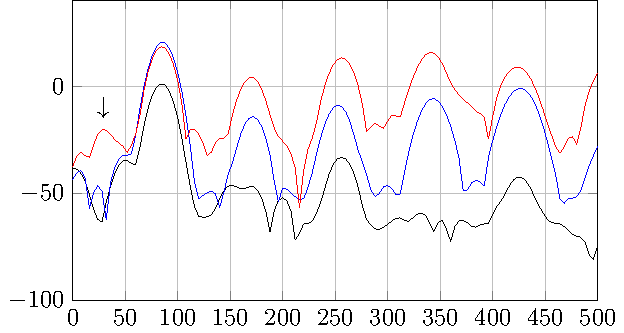
\includegraphics[width=0.6\textwidth]{FFT_hit}
%\end{figure}
%\begin{itemize}
%\item Sort: 0.005 Watt (81 dB SPL)
%\item Blå:  22 Watt (100 dB SPL)
%\item Rød:  294 Watt (105 dB SPL)
%
%\end{itemize}
%\end{frame}
%
%
%\subsection{Problemerne}
%\begin{frame}{Feedback system}{Problemerne}
%Følgende problemer ved feedback systemet:
%\begin{itemize}
%\item For dårlige sensorer
%\begin{itemize}
%\item Ikke præcise
%\item For meget støj
%\item For dyrer 
%\item Fejlmålinger
%\end{itemize}
%\item Ingen tendenser at spotte indtil et slag ramte = for sent
%\begin{itemize}
%\item Feedback tager for lang tid
%\end{itemize}
%\item Upraktisk at måle harmoniske toner 
%\begin{itemize}
%\item Ingen superpositions muligheder
%\item Fasen på signalerne passer ikke nødvendigvis
%\end{itemize}
%\end{itemize}
%\end{frame}
%
%%%%%%%%%%%%%%%%%
%
%\section{Feedforward system}
%
%\begin{frame}{Feedforward system}{Konceptet}
%
%\begin{figure}
%\centering
%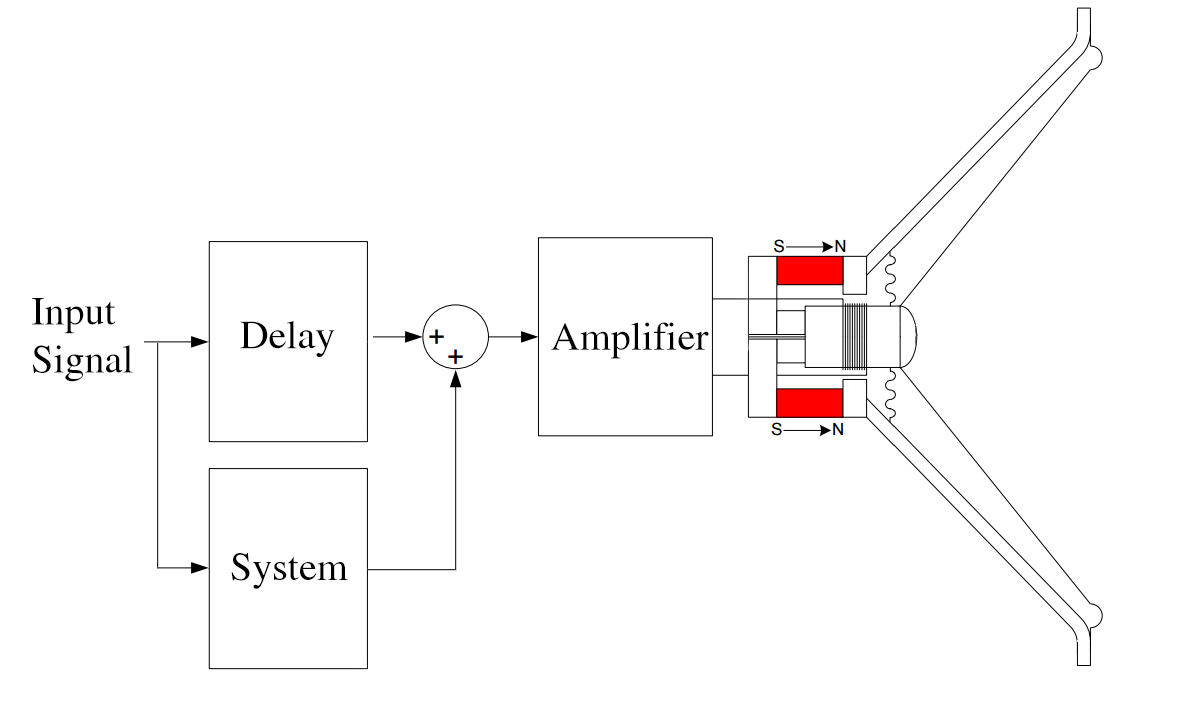
\includegraphics[width=0.9\textwidth]{Feedforward_Acc2}
%\end{figure}
%
%\end{frame}
%
%\begin{frame}{Feedforward system}{Overview}
%
%\begin{columns}
%  \begin{column}{0.70\textwidth}
%\begin{figure}
%\centering
%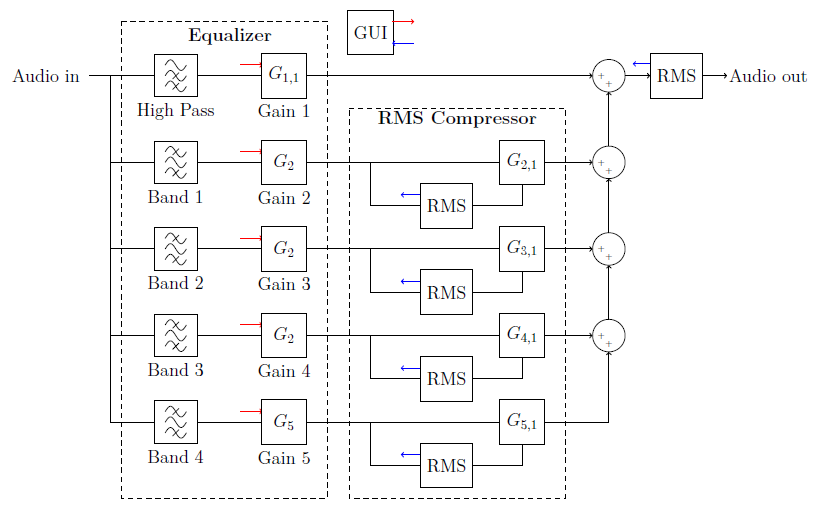
\includegraphics[width=0.85\textwidth]{Mainsystemoverview}
%\end{figure}
%  \end{column}
%  \begin{column}{0.30\textwidth}
%  \textbf{Systemet Overordnet}
%\begin{itemize}
%\item Grafisk Equalizer
%\item 4 Bånd i Bassen
%\begin{enumerate}
%\item 0   -   66 Hz
%\item 66  -  132 Hz
%\item 132 -  265 Hz
%\item 265 -  530 Hz
%\end{enumerate}
%\item RMS kompressor i 4 bånd
%\item RMS/Peak Limiter
%\item GUI til løbende justering
%\end{itemize}
%  \end{column}
%\end{columns}
%\end{frame}
%
%\subsection{Design Overvejelser}
%\begin{frame}{Feedforward system}{Design Overvejelser}
%\begin{columns}[t]
%  \begin{column}{0.50\textwidth}
%\textbf{Systemet skal:}
%\begin{itemize}
%\item Fungere ved lave frekvenser
%\item Have bånd til at måle frekvensområder
%\item Lineær fase
%\end{itemize}
%  \end{column}
%  \begin{column}{0.50\textwidth}
%  \textbf{Opnåes ved:}
%\begin{itemize}
%\item Realiseres som multi-rate
%\item Spektral subtraktion til at lave båndpas
%\item Opbygges af FIR filter
%\end{itemize}
%  \end{column}
%\end{columns}
%\vspace{5mm}
%\begin{block}{Overordnet set:}
%\begin{itemize}
%\item Downsampling til center frekvens på 3 kHz ved et 50-tap FIR filter
%\item x2 Downsampling 7 gange (x4,x8,x16,x32,x64)
%\item Indivudel kompressor i fire nederste bånd
%\end{itemize}
%\end{block}
%\end{frame}
%
%
%
%
%\subsection{Overordnet system}
%\begin{frame}{Feedforward system}{Systemet}
%
%\begin{columns}
%  \begin{column}{0.75\textwidth}
%\begin{figure}
%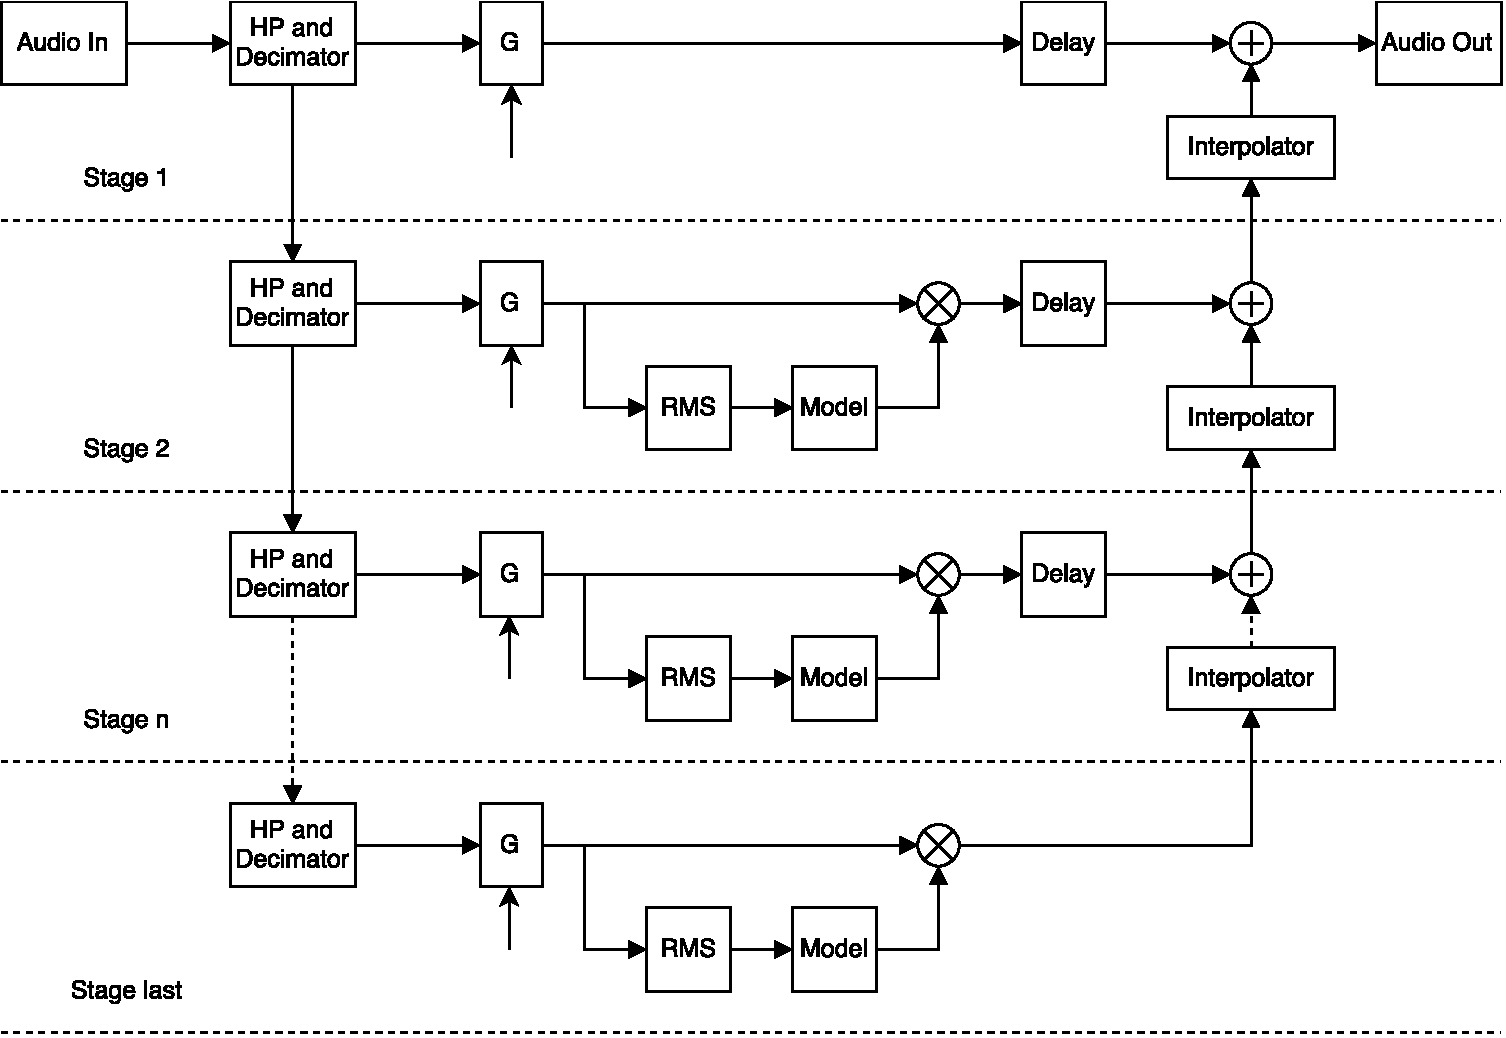
\includegraphics[width=\textwidth]{designRealBlock1}
%\end{figure}
%  \end{column}
%
%  \begin{column}{0.25\textwidth}
%  \textbf{Flow gennem system:}
%     \begin{enumerate}
%        \item Sample
%        \item Decimate
%        \item Spektral inversion
%        \item Påfør gain
%        \item Mål RMS
%        \item Påfør dæmpning
%        \item Interpolate
%        \item Summation
%     \end{enumerate}
%  \end{column}
%\end{columns}
%\end{frame}
%
%
%
%\subsection{Decimation}
%\begin{frame}{Feedforward system}{Decimator}
%
%\begin{columns}
%  \begin{column}{0.4\textwidth}
%\begin{figure}
%\centering
%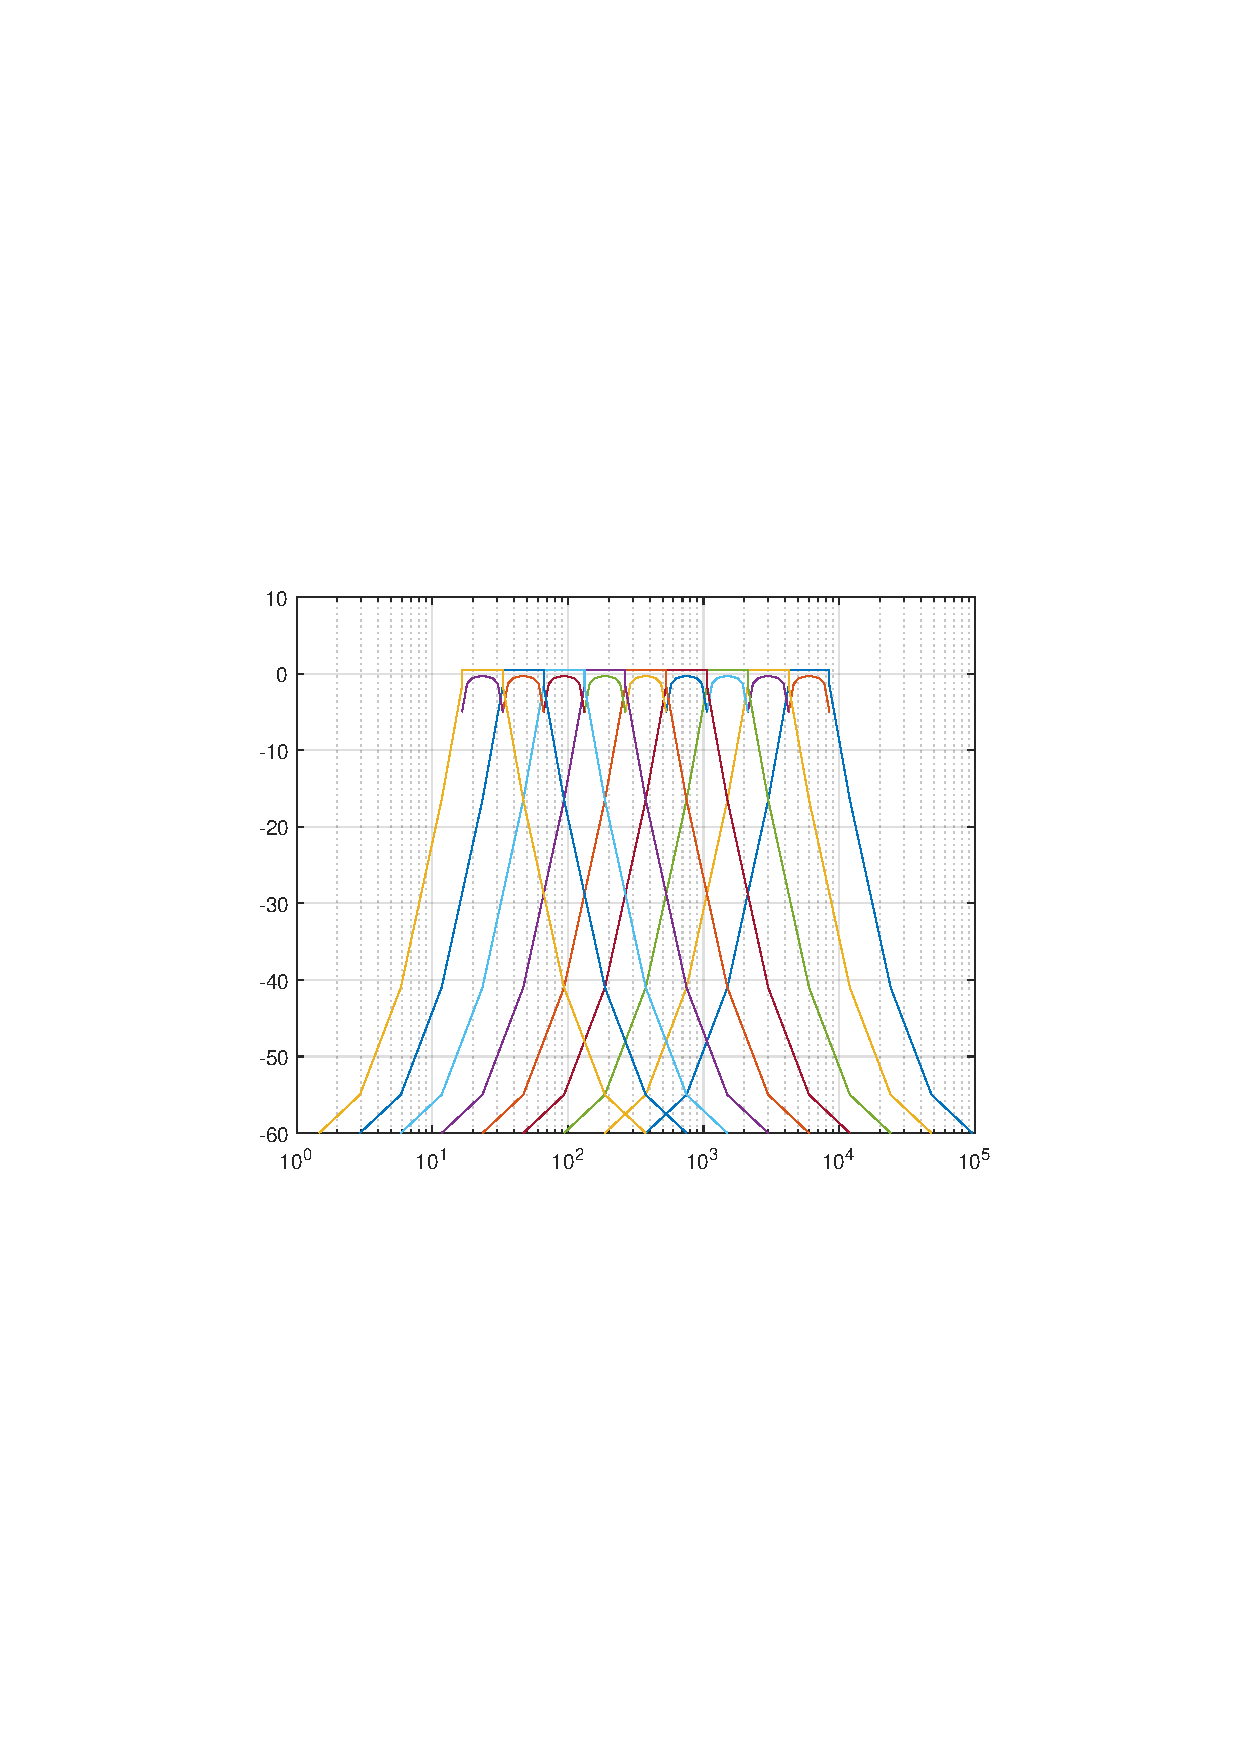
\includegraphics[width=\textwidth]{Bands}
%\end{figure}
%  \end{column}
%
%  \begin{column}{0.6\textwidth}
%\begin{itemize}
%\item 1 lavpas filter til båndpas
%\begin{itemize}
%\item Spektral subtraktion
%\end{itemize}
%\item 50. orden FIR
%\item Overholder IEC 6964 - Class 2 
%\end{itemize}
%\begin{figure}
%\centering
%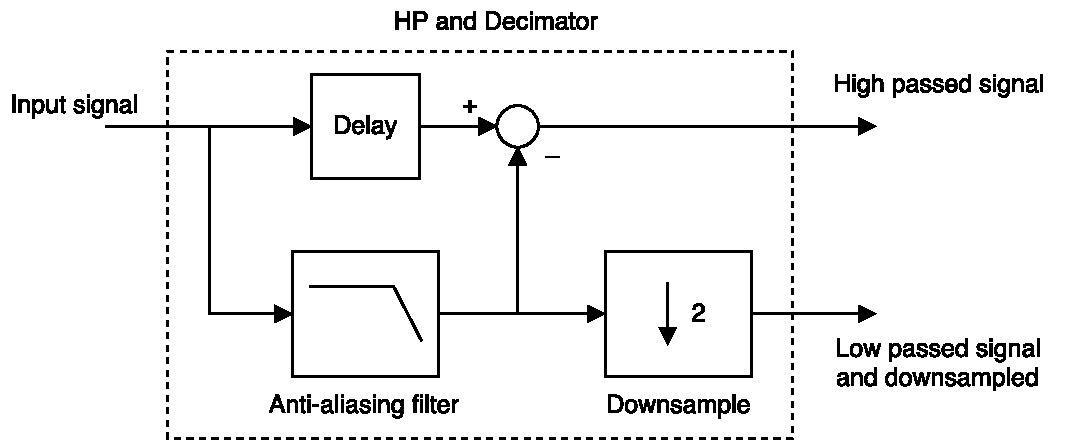
\includegraphics[width=\textwidth]{designRealDecimator}
%\end{figure}
%  \end{column}
%\end{columns}
%\end{frame}
%%%%%%%%%%%%%%%%%
%
%
%
%\subsection{RMS Compressor}
%\begin{frame}{Feedforward system}{RMS Compressor}
%
%\begin{columns}
%  \begin{column}{0.5\textwidth}
%\begin{figure}
%\centering
%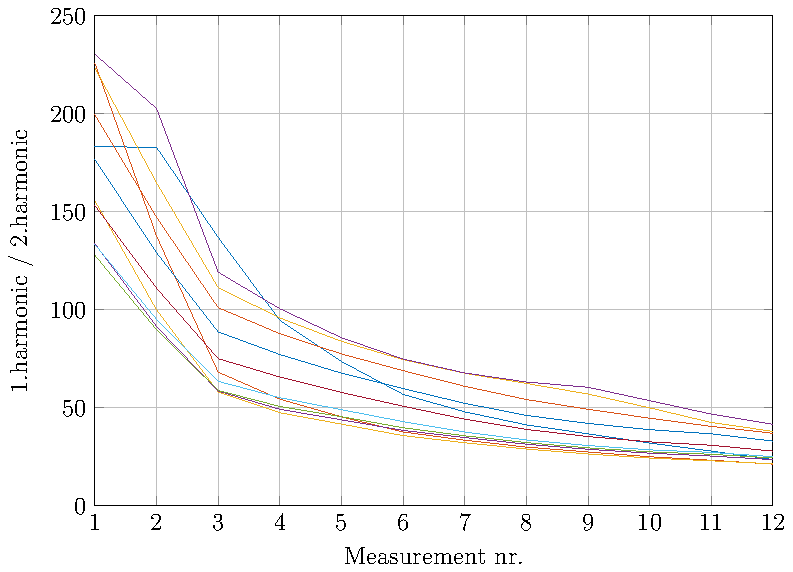
\includegraphics[width=0.7\textwidth]{comp_mic12All}
%\end{figure}
%\vspace{-5mm}
%\begin{figure}
%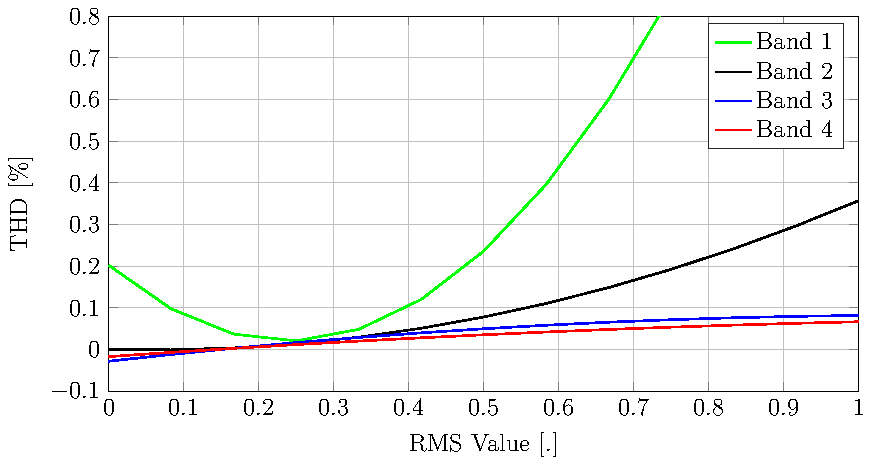
\includegraphics[width=0.8\textwidth]{BandModelCombine}
%\end{figure}
%  \end{column}
%  \begin{column}{0.5\textwidth}
%\begin{itemize}
%\item Dæmpning på op til 60 dB
%\item Opløsning på 1024 Steps
%\item Udskiftelig modeller
%\end{itemize}
%\begin{figure}
%\centering
%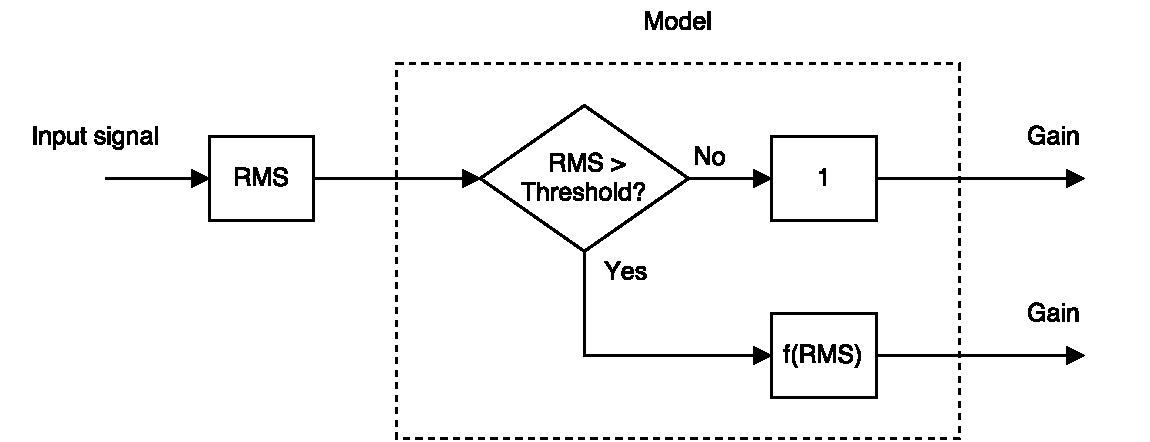
\includegraphics[width=\textwidth]{designRealRMS}
%\end{figure}
%  \end{column}
%\end{columns}
%
%\end{frame}
%
%
%
%
%\subsection{Interpolation}
%\begin{frame}{Feedforward system}{Interpolation}
%
%\begin{columns}
%  \begin{column}{0.4\textwidth}
%%\begin{figure}
%%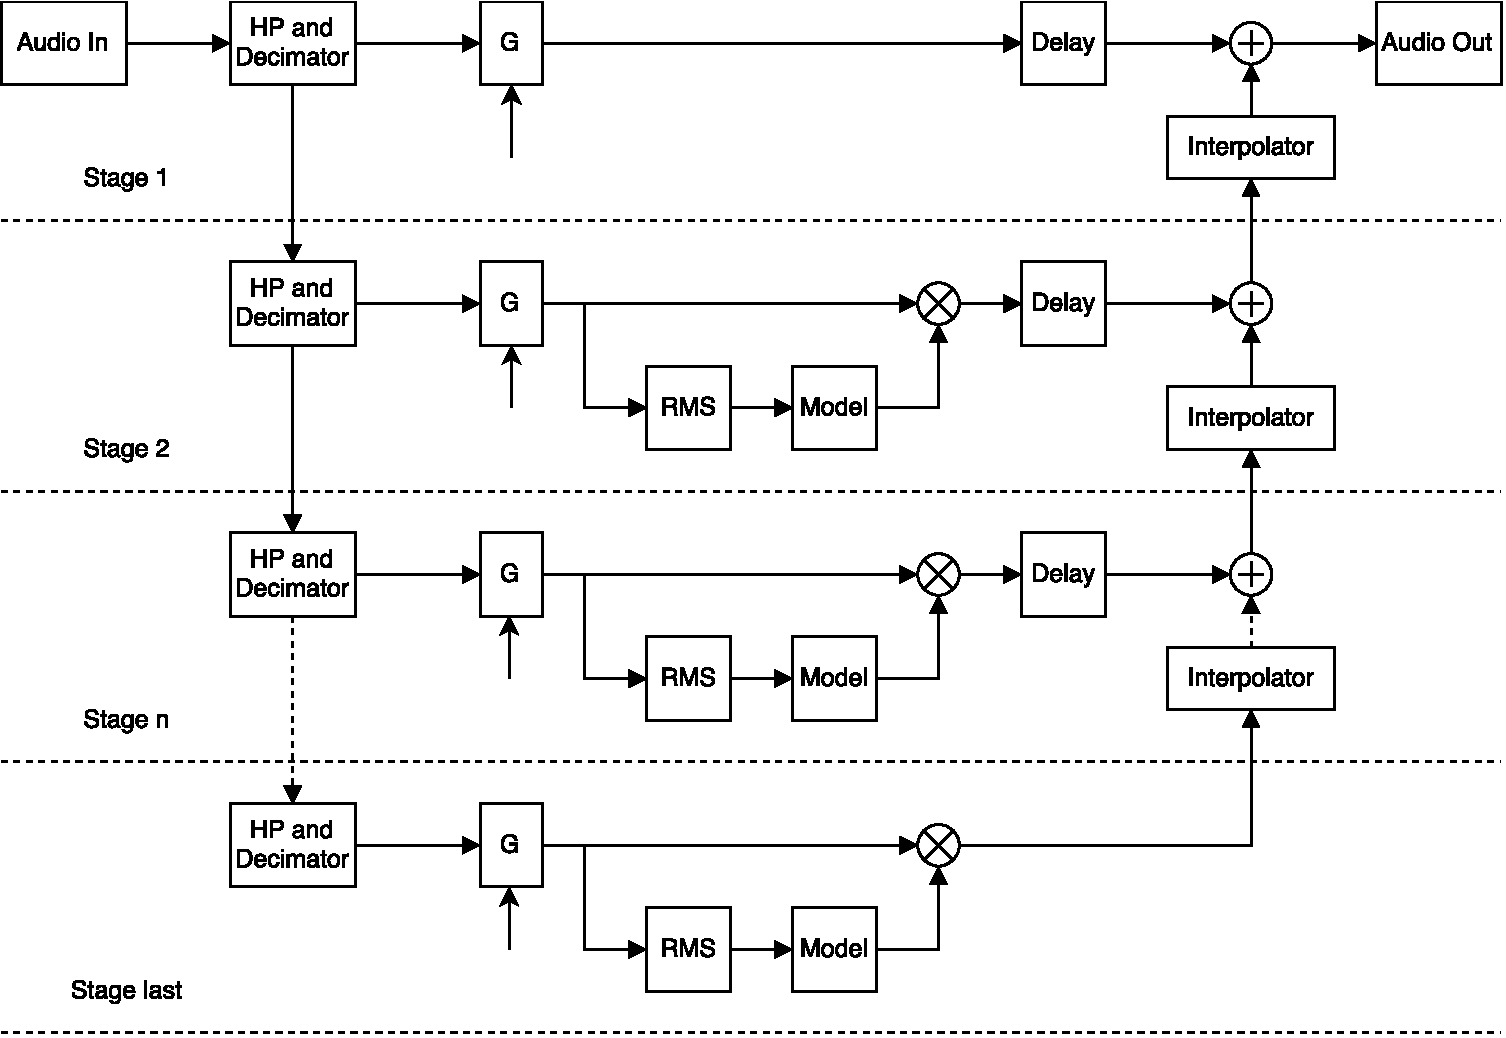
\includegraphics[width=0.9\textwidth]{designRealBlock1}
%%\end{figure}
%\begin{itemize}
%\item Zero-padding
%\item 48. Orden FIR
%\item Gain x2
%\end{itemize}
%  \end{column}
%
%  \begin{column}{0.6\textwidth}
%\begin{figure}
%\centering
%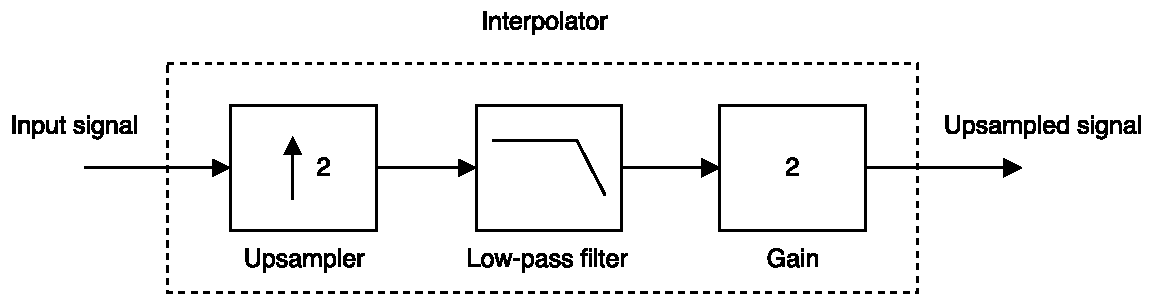
\includegraphics[width=\textwidth]{designRealInterpolator}
%\end{figure}
%  \end{column}
%\end{columns}
%
%\end{frame}
%
%
%
%\subsection{Simulering}
%\begin{frame}{Feedforward system}{Simulering}
%
%\begin{center}
%Simulering i MATLAB
%\end{center}
%
%\end{frame}
%
%\subsection{Opsumering}
%\begin{frame}{Feedforward system}{Opsumering}
%
%\begin{columns}[t]
%\begin{column}{0.40\textwidth}
%\textbf{Decimation/Interpolation:}
%\begin{itemize}
%\item Få instruktioner / Lav orden
%\item Billige FIR filter
%\item Mulighed for mere optimering
%\end{itemize}
%  \end{column}
%  \begin{column}{0.3\textwidth}
%\textbf{RMS Compressor:}
%\begin{itemize}
%\item Fleksible modeller
%\item Minimere hård limitering
%\item Fungere som både Peak og RMS
%\end{itemize}
%  \end{column}
%    \begin{column}{0.3\textwidth}
%\textbf{Overall:}
%\begin{itemize}
%\item Ingen støj
%\item Flat respons (+/- 1 dB)
%\end{itemize}
%  \end{column}
%\end{columns}
%
%\begin{block}{Kan Realiseres med:}
%\begin{itemize}
%\item Mulighed for 32-bit og 192 kHz
%\begin{itemize}
%\item Kun en ALU brugt
%\item 192 kHz vil kræve (x128,x256)
%\end{itemize}
%\end{itemize}
%\end{block}
%\vspace{-3mm}
%\begin{block}{Er Realiseret med:}
%\begin{itemize}
%\item Ca. 800 instruktioner.
%\item 16-bit og 48 kHz
%\item Peak limiter, RMS compressor og grafisk equalizer.
%\end{itemize}
%\end{block}
%
%\end{frame}
%
%
%\section{Demonstration}
%\begin{frame}{Feedforward system}{DEMO}
%
%\begin{center}
%DEMO\\
%\textit{Med forbehold}
%\end{center}
%\end{frame}
%
%\section{Spørgsmål og Evt.}
%% contact information
%\begin{frame}{Spørgsmål og Evt.}
%  \begin{center}
%Spørgsmål og Evt.
%  \end{center}
%\end{frame}





{\aauwavesbg
\begin{frame}[plain,noframenumbering]
  \finalpage{}
\end{frame}}
%%%%%%%%%%%%%%%%

\end{document}


%  \begin{block}{Global Installation}
%  \begin{itemize}
%     \item If you wish to make the theme globally available, you must put the files in your local latex directory tree. The location of the root of the local directory tree depends on the operating system and the latex distribution. On the following slides, you can read the instructions for some common setups.
%    \item When you download the theme, the four theme files are embedded in a directory structure (in the {\tt global} folder) ready to be copied directly to the root of your local directory tree.
%    \item On the following slides, we refer to this directory structure as {\tt <dirstruct>}. \alert{Note} that some parts of the directory may already exist if you have installed other packages in your local latex directory tree. If this is the case, you simply merge {\tt <dirstruct>} with your existing setup.
%  \end{itemize}
%  \end{block}